% !TEX program = xelatex
\documentclass[10pt,onecolumn]{article}

\usepackage[a4paper,margin=18mm,top=17mm,bottom=18mm]{geometry}
\raggedbottom
\renewcommand{\topfraction}{0.9}
\renewcommand{\floatpagefraction}{0.85}
\usepackage{microtype}
\usepackage{amsmath,amssymb}
\usepackage{siunitx}
\usepackage{booktabs}
\usepackage{tabularx}
\usepackage{array}
\usepackage{enumitem}
\usepackage{graphicx}
\usepackage[dvipsnames,svgnames,table]{xcolor}
\usepackage{tikz}
\usepackage[most]{tcolorbox}
\usepackage{titlesec}
\usepackage{fancyhdr}
\usepackage{hyperref}
\usepackage{caption}
\newcommand{\doi}[1]{DOI:~\href{https://doi.org/#1}{#1}}
\usepackage{float}

\usetikzlibrary{arrows.meta,calc,positioning,shapes.geometric,decorations.pathmorphing,backgrounds,fit}

\definecolor{ink}{HTML}{151B23}
\definecolor{titlebg}{HTML}{100880}
\definecolor{softink}{HTML}{263441}
\definecolor{muted}{HTML}{5C6875}
\definecolor{paper}{HTML}{F6F7F2}
\definecolor{panel}{HTML}{FFFFFF}
\definecolor{line}{HTML}{D8DEE5}
\definecolor{teal}{HTML}{007C77}
\definecolor{blue}{HTML}{245AA6}
\definecolor{gold}{HTML}{B86B00}
\definecolor{rose}{HTML}{A7354D}
\definecolor{green}{HTML}{23724A}
\definecolor{violet}{HTML}{5A4CA0}

\hypersetup{
  colorlinks=true,
  linkcolor=blue,
  citecolor=teal,
  urlcolor=gold,
  pdftitle={Wide-Field Spectroscopic and Imaging Cosmology Proposal for a 3.5-meter Segmented-Mirror Robotic Space Telescope},
  pdfauthor={Prepared proposal draft}
}

\pagestyle{fancy}
\fancyhf{}
\fancyhead[L]{\sffamily\footnotesize 3.5-meter Segmented-Mirror Robotic Space Telescope}
\fancyhead[R]{\sffamily\footnotesize Wide-Field Cosmology Proposal}
\fancyfoot[C]{\sffamily\footnotesize\thepage}
\renewcommand{\headrulewidth}{0.35pt}

\titleformat{\section}{\sffamily\Large\bfseries\color{ink}}{\thesection}{0.6em}{}
\titleformat{\subsection}{\sffamily\large\bfseries\color{blue}}{\thesubsection}{0.6em}{}
\titleformat{\subsubsection}{\sffamily\normalsize\bfseries\color{softink}}{\thesubsubsection}{0.6em}{}
\titlespacing*{\section}{0pt}{1.1em}{0.45em}
\titlespacing*{\subsection}{0pt}{0.85em}{0.3em}
\captionsetup{font={small,sf},labelfont={bf,color=blue}}
\setlist[itemize]{leftmargin=*,itemsep=2pt,topsep=3pt}
\setlist[enumerate]{leftmargin=*,itemsep=2pt,topsep=3pt}
\renewcommand{\arraystretch}{1.18}

\newcolumntype{Y}{>{\raggedright\arraybackslash}X}
\newcommand{\facility}{3.5-meter Segmented-Mirror Robotic Space Telescope}
\newcommand{\rsd}{redshift-space distortion}
\newcommand{\fsig}{f\sigma_8}
\newcommand{\degti}{deg$^2$}
\newcommand{\kms}{km\,s$^{-1}$}
\newcommand{\fovsmall}{$10'\!\times10'$}
\newcommand{\fovlarge}{$30'\!\times30'$}

\newtcolorbox{leadbox}[2][]{
  enhanced,
  colback=paper,
  colframe=#2,
  boxrule=0.9pt,
  arc=2mm,
  left=2.2mm,
  right=2.2mm,
  top=1.8mm,
  bottom=1.8mm,
  fonttitle=\sffamily\bfseries,
  coltitle=white,
  attach boxed title to top left={xshift=2mm,yshift=-2mm},
  boxed title style={colback=#2,arc=1.2mm,boxrule=0pt},
  #1
}

\newtcolorbox{metricbox}[1]{
  enhanced,
  colback=white,
  colframe=#1,
  boxrule=0.65pt,
  arc=1.3mm,
  left=1.8mm,
  right=1.8mm,
  top=1.6mm,
  bottom=1.6mm
}

\begin{document}

\thispagestyle{empty}
\begin{tikzpicture}[remember picture,overlay]
  \fill[titlebg] (current page.north west) rectangle ([yshift=-7.6cm]current page.north east);
  \fill[blue!55!black] ([yshift=-7.6cm]current page.north west) rectangle ([yshift=-7.9cm]current page.north east);
  \draw[teal,line width=1.0pt,opacity=0.80]
    ([xshift=0.8cm,yshift=-6.25cm]current page.north west)
    .. controls +(4.5,1.8) and +(-4.0,-1.2) ..
    ([xshift=20.4cm,yshift=-1.15cm]current page.north west);
  \draw[gold,line width=0.7pt,opacity=0.55]
    ([xshift=0.8cm,yshift=-6.75cm]current page.north west)
    .. controls +(5.0,1.4) and +(-5.0,-1.0) ..
    ([xshift=20.4cm,yshift=-2.0cm]current page.north west);
  \foreach \x/\y/\r/\c in {
    2.0/1.1/0.55/white,4.8/2.1/0.36/teal,7.8/0.9/0.42/white,
    11.5/1.8/0.34/gold,14.2/0.7/0.50/white,18.2/1.45/0.40/teal} {
    \fill[\c,opacity=0.25] ([xshift=\x cm,yshift=-\y cm]current page.north west) circle (\r mm);
  }
  \begin{scope}[shift={([xshift=16.05cm,yshift=-5.30cm]current page.north west)}]
    \def\hexrad{0.285}
    \foreach \q/\r/\col in {
      0/0/white,
      1/0/teal,0/1/blue,-1/1/gold,-1/0/rose,0/-1/violet,1/-1/green,
      2/0/teal,1/1/blue,0/2/gold,-1/2/rose,-2/2/violet,-2/1/green,
      -2/0/teal,-1/-1/blue,0/-2/gold,1/-2/rose,2/-2/violet,2/-1/green} {
      \pgfmathsetmacro{\cx}{sqrt(3)*\hexrad*(\q+0.5*\r)}
      \pgfmathsetmacro{\cy}{1.5*\hexrad*\r}
      \node[regular polygon,regular polygon sides=6,minimum size=0.57cm,rotate=30,
        fill=\col!24,draw=white!75,line width=0.35pt,opacity=0.95] at (\cx,\cy) {};
    }
    \draw[white,opacity=0.22,line width=0.6pt] (0,0) circle (1.55cm);
    \node[anchor=north,color=white!72,font=\sffamily\scriptsize] at (0,-1.95) {19-segment primary mirror};
  \end{scope}
\end{tikzpicture}

\vspace*{0.35cm}
{\sffamily\color{white}\fontsize{25}{30}\selectfont\bfseries Cosmology with a Wide-Field Spectroscopic and Imaging Survey}\\[1.2mm]
{\sffamily\color{white}\fontsize{16}{20}\selectfont with the \facility}\\[3mm]
{\sffamily\color{white!78}\large A one-column science proposal for a combined slitless-spectroscopy and deep-imaging survey}\\[10mm]

\begin{leadbox}[title=Executive Summary]{teal}
\textbf{The \facility\ is proposed as a robotic wide-field cosmology mission that combines native $R=1000$ slitless spectroscopy with deep wide-field imaging.}
The central science case is a dense emission-line galaxy redshift survey for BAO and redshift-space distortions, supported by supernova and quasar programs that exploit the stability, multiplexing, and repeatability of space operations. The supernova tier in particular measures the rest-frame $U$ and near-ultraviolet magnitudes that separate the optical twins at subgroup precision ($\sigma_m=0.10$\,mag) to $z\simeq0.9$--$1.1$ in its standard visits and to $z\simeq1.3$--$1.5$ in ten-hour stacks. The design assumes a crowded-field slitless environment from the start. Every science tile is observed in three orientations, approximately $0^\circ$, $45^\circ$, and $90^\circ$, so that spectral overlap can be solved by a joint scene-reconstruction algorithm. The flagship survey covers 100--300 \degti, requires the \fovlarge\ field for efficiency, and is complemented by a deep pencil-beam tier and a supernova time-domain tier. The same imaging runs as a blind low-surface-brightness census (UDGs, LSBGs, void dark galaxies) over the survey tiers and as targeted deep integrations on nearby clusters for intracluster light. Over the spectroscopic tiers the census uses emission-line redshifts to recover the low-surface-brightness population that is missing from the observed galaxy stellar mass function, turning its faint end into a selection-controlled test of stellar feedback. The same selection function, followed from field dwarfs through cluster and void environments, also supports a dark-matter microphysics program, testing cold, self-interacting, and fuzzy dark matter against dwarf-galaxy inner density structure and the abundance of low-mass halos.
\end{leadbox}

\vspace{2mm}
\begin{center}
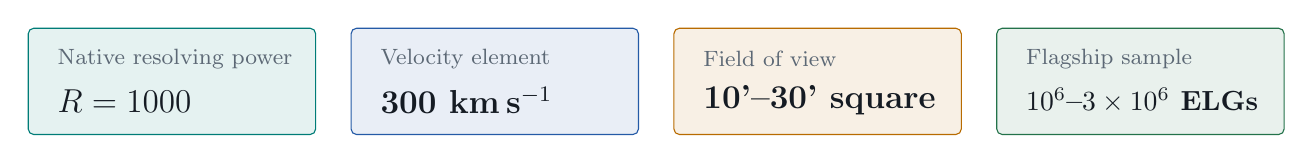
\begin{tikzpicture}[font=\sffamily]
  \foreach \x/\title/\val/\col/\vfont in {
    0/{Native resolving power}/{$R=1000$}/teal/\large,
    4.1/{Velocity element}/{300 \kms}/blue/\large,
    8.2/{Field of view}/{10'--30' square}/gold/\large,
    12.3/{Flagship sample}/{$10^6$--$3\times10^6$ ELGs}/green/\normalsize} {
    \fill[\col!10,draw=\col,rounded corners=2pt] (\x,0) rectangle ++(3.65,1.35);
    \node[anchor=west,color=muted,font=\footnotesize] at (\x+0.25,0.96) {\title};
    \node[anchor=west,color=ink,font=\bfseries\vfont] at (\x+0.25,0.43) {\val};
  }
\end{tikzpicture}
\end{center}

\section{Instrument Baseline}

The mission is designed around native $R=1000$ slitless spectroscopy because the leading cosmological measurements are controlled by survey volume, line identification, source confusion, and selection-function calibration. The highest-leverage observing mode is a repeatedly calibrated, wide-field map of emission-line galaxies, not precision internal kinematics for individual extended sources.

For a point source,
\begin{equation}
  \Delta v_{\rm FWHM}\simeq \frac{c}{R}
  \simeq 300\ {\rm km\,s^{-1}}\quad (R=1000).
\end{equation}
This is still not a peculiar-velocity measurement for individual galaxies. It is a redshift measurement feeding a statistical clustering analysis. RSD constrains $\fsig(z)$ through the anisotropic galaxy power spectrum $P(k,\mu)$ or correlation function. The dominant requirements are redshift success, purity, survey window control, and sufficient $nP$.

The most important instrumental change is spectral length. A constant-resolution spectrum over 0.3--3\,$\mu$m requires
\begin{equation}
  N_{\rm res}=R\ln\left(\frac{3}{0.3}\right)
  \simeq 2303\quad (R=1000),
\end{equation}
or about 4600 pixels at two pixels per resolution element. This is still too long for a single all-band slitless exposure in crowded fields. The baseline design is therefore band-limited, two-arm, and three-orientation from the start.

\begin{leadbox}[title=Baseline Configuration]{blue}
\begin{tabularx}{\textwidth}{@{}p{4.2cm}Y@{}}
\toprule
\textbf{Element} & \textbf{Adopted baseline for the proposal}\\
\midrule
Telescope & \facility; diffraction-limited segmented aperture, robotic survey operations.\\
Spectroscopy & Slitless grism/prism channels with native $R_{\rm point}=1000$ over band-limited filters.\\
Wavelength strategy & 0.3--1.0\,$\mu$m optical channel and 1.0--3.0\,$\mu$m near-IR channel; each channel divided into filters to limit spectrum length.\\
Field of view & \fovsmall\ threshold mode; \fovlarge\ survey mode and strongly preferred cosmology requirement.\\
Roll strategy & Three slitless orientations per science tile, approximately $0^\circ$, $45^\circ$, and $90^\circ$, to solve spectral overlap in crowded fields.\\
Direct imaging & Required for source detection, morphology priors, wavelength zero-points, and spectral-overlap modeling.\\
\bottomrule
\end{tabularx}
\end{leadbox}

\subsection{Two-Arm Slitless Spectrograph}

The spectrograph is a slitless two-arm system. A dichroic beam splitter sends 0.3--1.0\,$\mu$m light to the optical arm and 1.0--3.0\,$\mu$m light to the near-IR arm. Each arm uses band-limiting filters and a grism/prism disperser so that a crowded field does not produce decade-long spectra. The two arms can observe simultaneously when detector operations allow. Otherwise they are scheduled as matched visits with identical pointing and roll strategy. Because the near-infrared arm reaches $3.0\,\mu$m, its optics must be cooled so that the telescope thermal self-emission stays below the zodiacal background at the reddest wavelengths. The exposure-time calculation of Section~\ref{sec:etc} sets this requirement, with the optics reaching the background-limited floor across the full $1$--$3\,\mu$m band for an operating temperature $\lesssim200$\,K.

Two properties of grism dispersion shape the filter plan. The same band-limiting choice handles both. First, a grism disperses at nearly constant $\Delta\lambda$ per pixel rather than constant $R=\lambda/\Delta\lambda$, so the resolving power rises linearly across any one setting. The quoted $R=1000$ refers to the centre of each setting. Second, the diffraction orders of a grating overlap, since second-order light of wavelength $\lambda$ lands at the first-order position of $2\lambda$. The range that one setting can record free of cross-order contamination is accordingly at most one octave, $\lambda_{\max}\leq2\lambda_{\min}$. The survey therefore observes each arm through two band-limiting filters that each respect the octave limit, $0.36$--$0.70$ and $0.50$--$1.0\,\mu$m on the optical arm and $1.0$--$1.75$ and $1.6$--$3.0\,\mu$m on the near-infrared arm, the same order-sorting practice used by the HST, JWST, Euclid, and Roman slitless instruments. These are the two settings per wavelength channel assumed by every survey time estimate in this document. Within each setting the resolving power stays between $R\simeq670$ and $1330$ around the central $R=1000$, a first-order trace occupies about $1090$--$1330$ pixels at two pixels per resolution element. No transmitted wavelength has a second order inside the band of its own setting.

The choice of $R=1000$ is also robust against the natural suggestion of dispersing at higher resolution and binning the data down. In a slit spectrograph the sky disperses together with the source, which means higher resolution lowers the sky per pixel and later binning is nearly lossless. In slitless mode every pixel collects the sky of the \emph{entire} band-limiting filter regardless of the dispersion, and a grism of five times the resolution correspondingly spreads the same source counts over five times more sky-collecting pixels. Binning after detection cannot remove background photons that have already been recorded. The signal-to-noise of any binned quantity therefore degrades as the square root of the resolution ratio in the background-limited regime, a factor of $5^{1/2}\simeq2.2$ for $R=5000$ binned back to $R=1000$, equivalent to five times the exposure. The exposure-time calculator of Section~\ref{sec:etc} confirms the scaling directly. Raising the dispersion from $R=1000$ to $5000$ drops the binned synthetic-band S/N of a peak $z=1$ supernova from $12.2$ to $5.4$ in the same two-hour exposure. The emission-line depth for an extended source, by contrast, is identical at the two resolutions, because the effective resolution is already set by the source size (Section~\ref{sec:effres}). The five-fold growth of the trace-overlap rate in crowded fields and of the detector pixel count per setting also remains, since binning can undo neither. Higher resolution is therefore pure cost for the survey programs. The narrow-line science that would genuinely profit from it, the Ly$\alpha$ forest toward bright quasars, is better served by a small targeted mode than by raising the survey dispersion. This single native resolution is deliberately not re-tuned per companion program. Several are broad-feature science that $R=1000$ already resolves comfortably, or over-resolves, at no extra cost. Type~Ia supernova typing bins the native dispersion down to $R\simeq100$--$500$ without losing information (Section~\ref{sec:snia}), and the reionization damping wings and troughs are broad enough to need no higher resolution at all (Section~\ref{sec:lyaforest}). A few programs genuinely exceed the native resolving power, scoped around that limit rather than driving the survey design toward it. The Ly$\alpha$ forest above requires a dedicated $R\gtrsim30{,}000$ targeted mode, and strong-lens deflector dynamics (Section~\ref{sec:stronglens}) is restricted to an aperture-integrated, population-level velocity dispersion rather than a spatially resolved one. The pattern is consistent throughout. $R=1000$ is set by the flagship ELG survey, and each companion program is scoped to what that choice actually delivers for it, not the reverse.

\begin{figure}[tp]
\centering
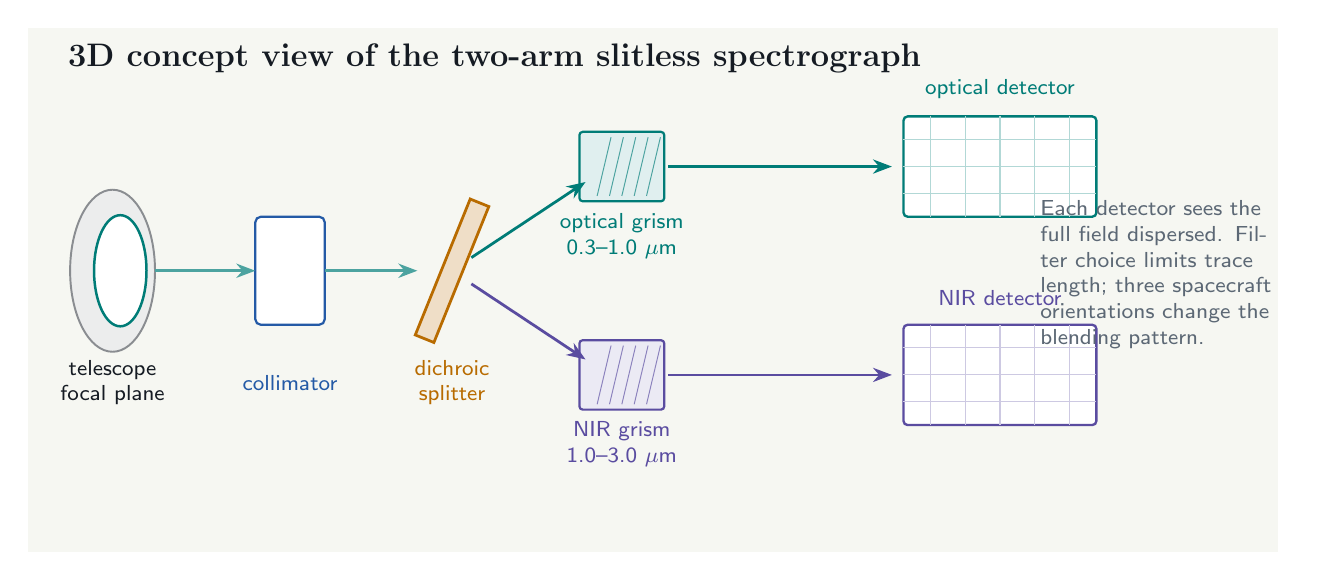
\begin{tikzpicture}[font=\sffamily\footnotesize,scale=0.98, every node/.style={transform shape}]
  \fill[paper] (-0.4,-0.45) rectangle (15.8,6.35);
  \node[anchor=west,font=\bfseries\large,color=ink] at (0,5.95) {3D concept view of the two-arm slitless spectrograph};

  \coordinate (tel) at (0.7,3.2);
  \coordinate (coll) at (3.0,3.2);
  \coordinate (dich) at (5.1,3.2);
  \coordinate (optg) at (7.3,4.55);
  \coordinate (nrg) at (7.3,1.85);
  \coordinate (optd) at (12.2,4.55);
  \coordinate (nrd) at (12.2,1.85);

  \draw[fill=ink!8,draw=ink!50,line width=0.7pt] (tel) ellipse (0.55 and 1.05);
  \draw[fill=white,draw=teal,line width=0.9pt] ($(tel)+(0.1,0)$) ellipse (0.34 and 0.72);
  \node[color=ink,align=center] at (0.7,1.75) {telescope\\focal plane};

  \draw[fill=white,draw=blue,line width=0.8pt,rounded corners=2pt] ($(coll)+(-0.45,-0.7)$) rectangle ($(coll)+(0.45,0.7)$);
  \node[color=blue,align=center] at (3.0,1.75) {collimator};

  \draw[fill=gold!22,draw=gold,line width=1.0pt,rotate around={-22:(dich)}] ($(dich)+(-0.13,-0.95)$) rectangle ($(dich)+(0.13,0.95)$);
  \node[color=gold,align=center] at (5.1,1.75) {dichroic\\splitter};

  \foreach \p/\name/\col/\txt in {optg/optical grism/teal/{0.3--1.0 $\mu$m},nrg/NIR grism/violet/{1.0--3.0 $\mu$m}} {
    \draw[fill=\col!12,draw=\col,line width=0.8pt,rounded corners=1.2pt] ($(\p)+(-0.55,-0.45)$) rectangle ($(\p)+(0.55,0.45)$);
    \foreach \dx in {-0.32,-0.16,0,0.16,0.32}
      \draw[\col!70,line width=0.35pt] ($(\p)+(\dx,-0.38)$) -- ($(\p)+(\dx+0.18,0.38)$);
    \node[color=\col,align=center] at ($(\p)+(0,-0.9)$) {\name\\\txt};
  }

  \foreach \p/\name/\col in {optd/optical detector/teal,nrd/NIR detector/violet} {
    \draw[fill=white,draw=\col,line width=0.85pt,rounded corners=1.5pt] ($(\p)+(-1.25,-0.65)$) rectangle ($(\p)+(1.25,0.65)$);
    \foreach \x in {-0.9,-0.45,0,0.45,0.9}
      \draw[\col!30] ($(\p)+(\x,-0.65)$) -- ($(\p)+(\x,0.65)$);
    \foreach \y in {-0.35,0,0.35}
      \draw[\col!30] ($(\p)+(-1.25,\y)$) -- ($(\p)+(1.25,\y)$);
    \node[color=\col,align=center] at ($(\p)+(0,1.0)$) {\name};
  }

  \draw[-{Stealth[length=2.4mm]},line width=1.1pt,color=white!30!teal] (1.25,3.2) -- (2.55,3.2);
  \draw[-{Stealth[length=2.4mm]},line width=1.1pt,color=white!30!teal] (3.45,3.2) -- (4.65,3.2);
  \draw[-{Stealth[length=2.4mm]},line width=1.0pt,color=teal] (5.35,3.37) -- (6.83,4.35);
  \draw[-{Stealth[length=2.4mm]},line width=1.0pt,color=violet] (5.35,3.03) -- (6.83,2.05);
  \draw[-{Stealth[length=2.4mm]},line width=1.0pt,color=teal] (7.9,4.55) -- (10.8,4.55);
  \draw[-{Stealth[length=2.4mm]},line width=1.0pt,color=violet] (7.9,1.85) -- (10.8,1.85);

  \node[anchor=west,text width=3.1cm,color=muted] at (12.6,3.15)
  {Each detector sees the full field dispersed. Filter choice limits trace length; three spacecraft orientations change the blending pattern.};
\end{tikzpicture}
\caption{Self-generated 3D-style spectrograph schematic. A dichroic splits the beam into optical and near-IR arms, each with its own band-limited slitless disperser and detector.}
\label{fig:spectrograph}
\end{figure}

\subsection{Crowded-Field Slitless Deblending}\label{sec:deblending}

The wide survey explicitly assumes crowded-field slitless spectroscopy. In dense extragalactic fields, a single dispersion direction is not sufficient. Spectra from neighboring galaxies will overlap. The overlap pattern will depend on wavelength, object morphology, and roll angle. The baseline extraction therefore uses a \textbf{multi-orientation scene-reconstruction algorithm} rather than independent one-dimensional extractions.

For each survey tile, the telescope obtains direct imaging plus slitless exposures at the nominal orientation and at rotated orientations separated by approximately $45^\circ$ and $90^\circ$. The $90^\circ$ observation provides near-orthogonal dispersion while the $45^\circ$ observation changes the blending pattern for pairs that remain blended in the orthogonal pair. The extraction pipeline then solves a joint forward model:
\begin{equation}
  \mathbf{d}_{r}=\mathbf{A}_{r}(\mathbf{x},\mathbf{m},\lambda)\,\mathbf{s}+\mathbf{n}_{r},
  \qquad r\in\{0^\circ,45^\circ,90^\circ\},
  \label{eq:scene}
\end{equation}
where $\mathbf{d}_{r}$ is the detector image at roll/orientation $r$, $\mathbf{s}$ is the set of object spectra, and $\mathbf{A}_{r}$ is the orientation-dependent projection operator built from the direct-image catalog, morphology model, trace solution, PSF, and wavelength calibration. The final spectra are recovered by a regularized joint fit over all orientations with covariance and contamination flags propagated into the redshift catalog. Objects that remain degenerate after the three-angle fit are not forced into the cosmology sample. They are assigned lower redshift purity or excluded by the survey mask.

The most cost-effective wide-survey choice is three roll orientations. Two nearly orthogonal orientations are the minimum useful configuration, but they leave a non-negligible class of pair geometries, detector defects, and extended-source self-blends with ambiguous solutions. A third roll, separated by roughly $45^\circ$ from the orthogonal pair, changes the blending pattern without multiplying the program into a deep-field campaign. Additional rolls are scientifically useful only for reference fields, ultra-deep calibration fields, or unusually crowded targets, because their survey-area cost is linear while the deblending gain becomes incremental.

\begin{table}[tp]
\centering
\sffamily\small
\begin{tabularx}{\textwidth}{@{}c p{3.2cm} Y Y@{}}
\toprule
\textbf{Rolls} & \textbf{Survey role} & \textbf{Deblending value} & \textbf{Cost judgment}\\
\midrule
1 & Not acceptable for cosmology & Cannot distinguish many spectral overlaps from real lines; poor independent cross-check. & Lowest cost but high redshift-failure and contamination risk.\\
2 & Minimum operational mode & Near-orthogonal pair resolves many overlaps and morphology projections. & Useful fallback, but still vulnerable to pairs blended in both directions.\\
3 & Baseline for wide BAO/RSD & Adds a different blending pattern; supports cross-checking by omitting one roll and robust contamination flags. & Best cost-performance point for the flagship survey.\\
4+ & Calibration/deep fields & Improves posterior sampling, rare degeneracies, and pipeline robustness tests. & Diminishing returns for the wide tier; reserve for reference fields.\\
\bottomrule
\end{tabularx}
\caption{Cost-benefit logic for the number of slitless roll orientations. The proposal adopts three rolls for the wide cosmology survey and uses additional rolls only where calibration value exceeds lost survey area.}
\label{tab:rollcost}
\end{table}

The baseline deblending pipeline uses the most established approach for precision slitless work. This approach combines calibrated forward modeling, simultaneous fitting of all cataloged sources, and regularized sparse linear inversion across all rolls and dithers. This follows the operational logic of HST slitless extraction software, where direct-image positions, morphology, trace solutions, flat-field cubes, and contamination models define the extraction geometry \cite{axe2009}. It also follows the LINEAR formalism, where all transformations between direct-image sources and dispersed pixels are assembled into a large sparse linear system solved by LSQR \cite{linear2018}. The same principle is used in crowded-field 3D spectroscopy. Spectra are extracted by fitting many sources simultaneously with a wavelength-dependent PSF and an external high-resolution catalog prior \cite{kamann2013,husser2016}. Machine learning is therefore not the primary deblender. It plays a constrained, supporting role for catalog quality assurance, missing-neighbor discovery, trace-mask generation, artifact rejection, and flagging of high-contamination pixels. Convolutional or instance-segmentation networks can flag these inputs following astronomical Mask R-CNN deblending work \cite{burke2019}. Bayesian or variational modules can attach posterior uncertainties to flux, contamination fraction, and redshift purity \cite{liu2021}. Non-negative matrix factorization can be tested for unresolved background, nebular components, and calibration crosstalk \cite{horstman2022}. Generative models, including diffusion, are not part of the baseline cosmology extraction unless they are constrained to reproduce the detector pixels through the calibrated forward model and pass injection-recovery bias tests. The success criterion is therefore not visual cleanliness. It is recovered line flux bias, redshift failure rate, contamination covariance, and injection-recovery completeness as functions of neighbor separation, magnitude contrast, morphology, and roll geometry.

The machine-learning literature on deblending spans several families. It is useful to place each relative to this calibrated forward model. The first is constrained matrix factorization, exemplified by SCARLET, which models every source as a small number of components, each the product of a spectral energy distribution and a non-parametric spatial profile. The method imposes physical constraints such as non-negativity, monotonicity from the peak, and symmetry to make the separation well posed \cite{scarlet2018}. It is a semi-parametric optimization method rather than a trained network. It is the production deblender of the Rubin Observatory Science Pipelines. The second family is deep generative priors. Variational autoencoders \cite{arcelin2021,lanusse2021}, normalizing flows, and more recently score-based and diffusion models learn a distribution over galaxy morphologies from training data, using it to regularize the separation, which improves the recovery of heavily overlapping pairs. The third family is instance-segmentation networks such as Mask R-CNN that detect and mask overlapping sources at the pixel level \cite{burke2019}. The fourth is probabilistic and variational catalog inference that returns full posteriors on source positions and fluxes \cite{liu2021}. For a slitless cosmology survey the decisive property is not raw image-plane separation quality but control of line-flux bias. Therefore, the present baseline uses these methods as priors and quality checks inside the forward model rather than as standalone image cleaners. Any learned prior must reproduce the detector pixels through the same calibrated operator and pass injection-recovery tests before it enters the cosmology path.

The two wide-field space missions closest to this concept have made deliberately different choices. Both inform the baseline. Euclid performs its photometric source separation by model fitting, fitting Sersic and disk-plus-Sersic profiles to every object simultaneously with the SourceXtractor++ package. This approach was validated in the Euclid Morphology Challenge, which showed it recovers structural parameters reliably across billions of galaxies \cite{sourcext2020,euclidmorph2023}. Its near-infrared slitless spectroscopy is then extracted by a forward model that incorporates the direct-image morphology of each source as a prior, the same logic adopted here. Roman extracts its grism spectra with pyLINEAR, the sparse linear inversion which assembles every transformation between direct-image sources and dispersed pixels into one large system \cite{linear2018,wang2021}. Its supernova program has already demonstrated the multi-roll extension, reconstructing a three-dimensional scene from slitless spectra taken at all available roll angles so that host-galaxy light can be separated from the supernova \cite{roman3d2026}. Forward-model emulators such as ESpRESSO now generate realistic Roman slitless scenes for training and validating these pipelines \cite{espresso2024}. Rubin, whose data are imaging rather than slitless, deblends with the constrained SCARLET factorization \cite{scarlet2018}. The present proposal sits closest to the Roman lineage, because its science is slitless and its defining asset is multi-orientation coverage. Hence, it adopts the Roman and HST forward model of Eq.~\eqref{eq:scene} as the baseline, using the Euclid model-fitting priors and the Rubin and generative machine-learning methods as constrained support.

\begin{figure}[tp]
\centering

\includegraphics[width=\textwidth]{slitless_scene_sim.png}
\caption{Simulated crowded-field slitless exposures at the survey baseline, $0.11''$ pixels and the $1.0$--$1.75\,\mu$m band-limited setting with $R=1000$ at the setting centre, which gives constant dispersion and $1091$-pixel first-order traces. Sources follow deep near-infrared counts, $40$ per arcmin$^2$ over $18.5<m_{\rm AB}<24.5$, with FSPS galaxy template spectra at $0.4<z<2.2$. \emph{Top left}: the direct image of the displayed $88''\times88''$ field. \emph{Other panels}: the same field dispersed at the three survey roll angles, with traces from sources outside the crop entering it as on a real detector. Every source becomes a long one-sided trace, emission lines appear as compact knots on the traces, and neighbouring spectra overlap heavily at any single orientation. Rotating the dispersion by $45^\circ$ and $90^\circ$ changes which pairs overlap. That redundancy is what the joint scene reconstruction of Eq.~\eqref{eq:scene} exploits to assign flux and flag irreducible blends before cosmological analysis. This panel illustrates the overlap geometry and the method, not a completed recovery-statistics validation. The purity, completeness, and flux-bias numbers that would demonstrate the method at survey scale are the output of the End-to-End Validation suite of Section~\ref{sec:e2eval}, not yet produced from a survey-scale simulation.}
\label{fig:crowded}
\end{figure}

The three-roll strategy above accepts whole-field overlap and resolves it statistically after the fact. An image slicer is a complementary option for the fields where crowding is worst. It cuts the two-dimensional focal-plane image into narrow slices, reformats the slices end to end into one pseudo-slit, and disperses that pseudo-slit as a single spectrum. Sources in different slices can never overlap. Only sources sharing, or adjacent to, the same slice can still blend in wavelength. This is a substantially smaller overlap graph than the whole-field blending of Figure~\ref{fig:crowded}. Image slicers already fly on integral-field spectrographs, including the JWST NIRSpec IFU mode \cite{boker2022}. The concept itself is therefore flight-proven. Adding one across the full wide-tier field of view is a substantial optical and mechanical addition which this proposal does not design or cost here. The more direct application is the medium, deep, and ultra-deep tiers, where the source density is highest and the completeness calibration is most sensitive to blending. For those fields, an image-slicer front end is a design direction worth carrying into a future trade study, not a baseline commitment of this proposal.

\begin{figure}[tp]
\centering

\includegraphics[width=\textwidth]{hsc_slicer_demo.png}
\caption{An image-slicer alternative to whole-field slitless dispersion, tested on a simulated scene built from real measurements rather than the synthetic random population of Figure~\ref{fig:crowded}. Every source's position, brightness, size, ellipticity, and position angle is measured directly from the Subaru HSC-SSP deep image of the SXDS/UDS/XMM-LSS deep-tier anchor \cite{aihara2018}, then rendered through this concept's own $0.11''$ pixels and diffraction-limited PSF rather than shown as the raw HSC pixels. Each row disperses the same reconstructed scene at one of the three survey roll angles, $0^\circ$, $45^\circ$, and $90^\circ$. \emph{Left}: the reconstructed direct image, cut into five horizontal slices. \emph{Right}: those slices reformatted end to end into one pseudo-slit (bottom, true pixel scale, not magnified) and dispersed together into a single spectrum (top, wavelength increasing upward), with the same instrument model and display contrast as Figure~\ref{fig:crowded} ($0.11''$ pixels, $1.0$--$1.75\,\mu$m, $R=1000$). Dashed lines mark each slice's own segment of the combined frame. Blending is confined to neighbours sharing, or adjacent to, the same slice. Sources in different slices never overlap at any roll angle. The slice count (five) and the projection of each source's elliptical profile onto the slit's spatial axis are simplifications for a clear illustration, not an optical design of a real image slicer.}
\label{fig:slicer}
\end{figure}

\subsection{Effective Resolution for Galaxies}\label{sec:effres}

The resolving power seen by an extended galaxy is reduced by morphology along the dispersion axis:
\begin{equation}
  R_{\rm eff}\simeq R_{\rm point}
  \frac{\theta_{\rm PSF}}{(\theta_{\rm PSF}^2+\theta_{\rm src,\parallel}^2)^{1/2}} .
  \label{eq:reff1000}
\end{equation}
At 1\,$\mu$m, a 3.5 m diffraction-limited telescope has a PSF FWHM of order $0.06''$. With $R_{\rm point}=1000$, Eq.~(\ref{eq:reff1000}) gives $R_{\rm eff}\simeq510$ for a $0.10''$ emitting region and $R_{\rm eff}\simeq290$ for a $0.20''$ emitting region. This is acceptable for ELG redshift surveys, but it means that precision internal kinematics of extended galaxies are not part of the flagship requirement.

Extended galaxies also create a second, internal deblending problem. Different parts of the same galaxy are projected to different detector pixels along the dispersion direction. Therefore, spatial structure is mixed with wavelength. This morphology-induced self-blending is handled inside the same calibrated forward model, not by a separate image-cleaning step. The direct image supplies a wavelength-zero-point prior, segmentation map, Sersic or multi-component morphology, and clump masks. For galaxies whose emission-line morphology is not well represented by the broadband continuum, the pipeline fits a small number of internal components,
\begin{equation}
  \mathbf{d}_{r,g} =
  \sum_{c=1}^{N_c}
  \mathbf{A}_{r,g,c}(\mathbf{x}_{g,c},\mathbf{m}_{g,c},\lambda)\,
  \mathbf{s}_{g,c}
  +\mathbf{n}_{r,g},
  \label{eq:scenecomp}
\end{equation}
where $g$ labels the galaxy and $c$ labels internal components such as disk, bulge, or star-forming knots. Equation~\eqref{eq:scenecomp} is not a second, independent model but the scene model of Eq.~\eqref{eq:scene} extended one level deeper. The single per-object spectrum $\mathbf{s}$ that galaxy $g$ contributes to Eq.~\eqref{eq:scene} is resolved here into a sum over its internal components $\mathbf{s}_{g,c}$, each with its own projection operator $\mathbf{A}_{r,g,c}$. The between-object and within-object terms are solved together in one linear system rather than in two separate passes. This nesting is the extended-source analogue of the LINEAR sparse forward model and the aXe morphology-based extraction geometry \cite{axe2009,linear2018}. The CSST slitless emulator similarly treats galaxy size, Sersic index, position angle, and axis ratio as drivers of slitless self-broadening \cite{cess2024}. The science catalog therefore reports $R_{\rm eff}$, line-flux covariance, morphology flags, and a self-blending quality flag. Objects whose redshift or line flux changes significantly when the morphology prior, component number, or omitted roll angle is varied are retained for ancillary science but excluded from the cosmology-grade BAO/RSD sample.

\begin{figure}[tp]
\centering
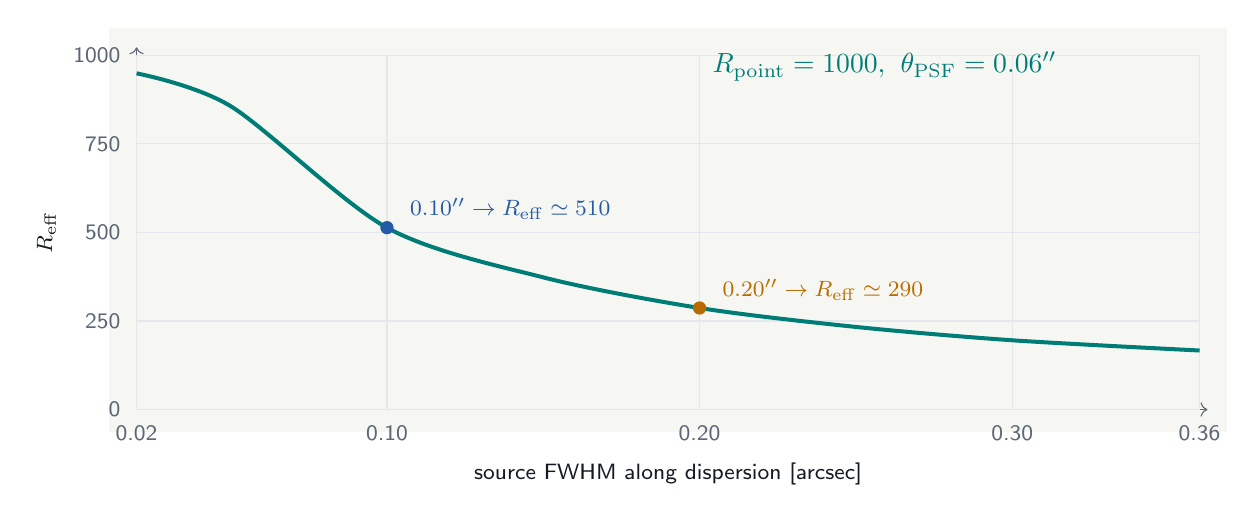
\begin{tikzpicture}[font=\sffamily\footnotesize]
  \def\w{13.5}
  \def\h{4.5}
  \fill[paper] (-0.35,-0.28) rectangle (\w+0.35,\h+0.35);
  \draw[->,color=muted] (0,0) -- (\w+0.1,0);
  \draw[->,color=muted] (0,0) -- (0,\h+0.1);
  \foreach \y/\lab in {0/0,1.125/250,2.25/500,3.375/750,4.5/1000} {
    \draw[line!70] (0,\y) -- (\w,\y);
    \node[anchor=east,color=muted] at (-0.08,\y) {\lab};
  }
  \foreach \x/\lab in {0/0.02,3.18/0.10,7.15/0.20,11.12/0.30,13.5/0.36} {
    \draw[line!70] (\x,0) -- (\x,\h);
    \node[anchor=north,color=muted] at (\x,-0.08) {\lab};
  }
  \draw[teal,line width=1.45pt,smooth]
    plot coordinates {(0,4.27) (1.2,3.85) (3.18,2.31) (5.16,1.68) (7.15,1.29) (9.13,1.05) (11.12,0.88) (13.5,0.75)};
  \fill[blue] (3.18,2.31) circle (2.4pt);
  \fill[gold] (7.15,1.29) circle (2.4pt);
  \node[anchor=west,color=blue] at (3.35,2.55) {$0.10''\rightarrow R_{\rm eff}\simeq510$};
  \node[anchor=west,color=gold] at (7.32,1.52) {$0.20''\rightarrow R_{\rm eff}\simeq290$};
  \node[anchor=south,color=teal,font=\bfseries] at (9.5,4.05) {$R_{\rm point}=1000,\ \theta_{\rm PSF}=0.06''$};
  \node[anchor=north,color=ink] at (0.5*\w,-0.55) {source FWHM along dispersion [arcsec]};
  \node[rotate=90,anchor=south,color=ink] at (-0.9,0.5*\h) {$R_{\rm eff}$};
\end{tikzpicture}
\caption{At $R=1000$, morphology sets the effective resolution for galaxies. The relevant design goal is robust redshift recovery, not galaxy internal kinematics.}
\label{fig:reff1000}
\end{figure}

\subsection{Field of View as a Science Requirement}

The field of view changes the mission from a deep-field spectroscopic facility into a cosmological surveyor. The two allowed field sizes differ by a factor of nine in area:
\begin{align}
  A(10'\times10') &= 100\ {\rm arcmin^2}=0.0278\ {\rm deg^2},\\
  A(30'\times30') &= 900\ {\rm arcmin^2}=0.2500\ {\rm deg^2}.
\end{align}
For a 100 \degti survey, the threshold field requires roughly 3600 pointings before the required three orientations and dithers while the maximum field requires 400. For 300 \degti, those numbers become 10,800 and 1200. Including the three slitless orientations, the raw spectroscopic visit count is multiplied by three. The \fovsmall\ mode is useful for deep calibration fields and time-domain fields. The \fovlarge\ mode should be treated as the cosmology survey requirement.

\begin{figure}[tp]
\centering
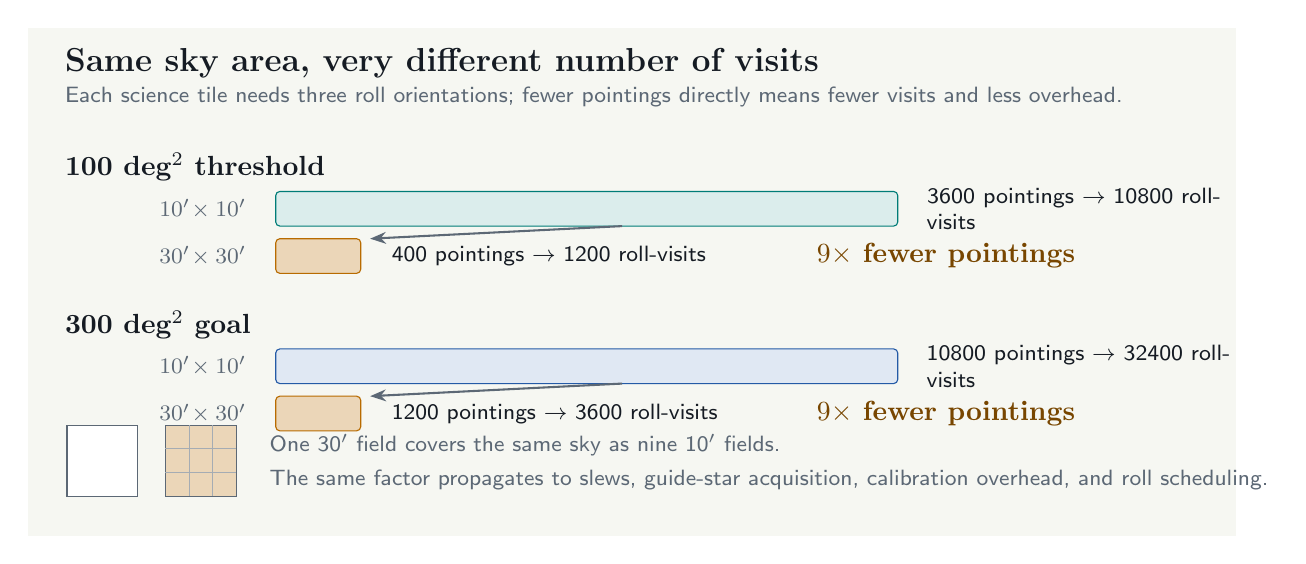
\begin{tikzpicture}[font=\sffamily\footnotesize]
  \fill[paper] (-0.35,-0.45) rectangle (15.0,6.0);
  \node[anchor=west,font=\bfseries\large,color=ink] at (0,5.55) {Same sky area, very different number of visits};
  \node[anchor=west,color=muted] at (0,5.12) {Each science tile needs three roll orientations; fewer pointings directly means fewer visits and less overhead.};

  \foreach \y/\survey/\smallp/\smallv/\largep/\largev/\col in {
    3.45/{100 deg$^2$ threshold}/3600/10800/400/1200/teal,
    1.45/{300 deg$^2$ goal}/10800/32400/1200/3600/blue} {
    \node[anchor=west,font=\bfseries,color=ink] at (0,\y+0.78) {\survey};
    \node[anchor=east,color=muted] at (2.55,\y+0.25) {\fovsmall};
    \node[anchor=east,color=muted] at (2.55,\y-0.35) {\fovlarge};

    \fill[\col!14,draw=\col,rounded corners=1.5pt] (2.8,\y+0.03) rectangle (10.7,\y+0.47);
    \fill[gold!28,draw=gold,rounded corners=1.5pt] (2.8,\y-0.57) rectangle (3.88,\y-0.13);

    \node[anchor=west,color=ink,text width=3.8cm] at (10.95,\y+0.25) {\smallp\ pointings $\rightarrow$ \smallv\ roll-visits};
    \node[anchor=west,color=ink] at (4.15,\y-0.35) {\largep\ pointings $\rightarrow$ \largev\ roll-visits};
    \node[anchor=west,font=\bfseries,color=gold!65!black] at (9.55,\y-0.35) {$9\times$ fewer pointings};

    \draw[-{Stealth[length=2mm]},color=muted,line width=0.75pt] (7.2,\y+0.03) -- (4.0,\y-0.13);
  }

  \begin{scope}[xshift=0.15cm,yshift=0.05cm]
    \draw[draw=muted,fill=white] (0,0) rectangle (0.9,0.9);
    \draw[draw=muted,fill=gold!28] (1.25,0) rectangle (2.15,0.9);
    \foreach \xx in {1.55,1.85} \draw[muted!55] (\xx,0) -- (\xx,0.9);
    \foreach \yy in {0.30,0.60} \draw[muted!55] (1.25,\yy) -- (2.15,\yy);
    \node[anchor=west,color=muted] at (2.45,0.65) {One 30$'$ field covers the same sky as nine 10$'$ fields.};
    \node[anchor=west,color=muted] at (2.45,0.20) {The same factor propagates to slews, guide-star acquisition, calibration overhead, and roll scheduling.};
  \end{scope}
\end{tikzpicture}
\caption{Field-of-view scaling for the wide RSD survey. The \fovlarge\ mode covers the same sky with one ninth as many pointings as \fovsmall. After the required three roll orientations, a 100 deg$^2$ survey needs about 1200 rather than 10,800 slitless visits.}
\label{fig:fov}
\end{figure}

\subsection{Sensitivity and the Exposure-Time Calculator}\label{sec:etc}

The sensitivity of the two-arm slitless spectrograph, and with it the survey planning depth adopted in Section~\ref{sec:elgdepth} (Eq.~\eqref{eq:f5sigma}), follows from a detector-level photon budget. It is worth deriving that depth from first principles and confirming both its value and its background-limited time scaling. For an emission line of flux $F_{\rm line}$ observed at wavelength $\lambda$, the number of detected photo-electrons accumulated over a total exposure $t$ is
\begin{equation}
  S=F_{\rm line}\,A_{\rm tel}\,\eta\,t\,\frac{\lambda}{hc},
  \label{eq:etcsig}
\end{equation}
where $A_{\rm tel}$ is the effective collecting area, $\eta$ is the end-to-end throughput including optics, disperser, and detector quantum efficiency, and $\lambda/hc$ converts line energy to photon number. In a slitless spectrograph a uniform sky disperses onto every detector pixel across the full band-limiting filter. Hence, the diffuse background collected per pixel per second is
\begin{equation}
  B_{\rm pix}=\bar i_{\rm sky}\,A_{\rm tel}\,\eta\,\Omega_{\rm pix}\,\Delta\lambda_{\rm filt}\,\frac{\lambda}{hc},
  \label{eq:etcbg}
\end{equation}
where $\bar i_{\rm sky}$ is the mean sky surface brightness per unit wavelength, $\Omega_{\rm pix}$ is the pixel solid angle, and $\Delta\lambda_{\rm filt}$ is the filter bandwidth that the proposal imposes to keep slitless traces short. The line falls on $n_{\rm pix}$ pixels, set by the source size along the cross-dispersion direction times the resolution-element width. Adding source shot noise, sky, dark current $D$, and read noise $\sigma_{\rm read}$ over $n_{\rm read}$ reads in quadrature gives the total variance
\begin{equation}
  N^2=S+B_{\rm pix}\,n_{\rm pix}\,t+D\,n_{\rm pix}\,t+n_{\rm read}\,n_{\rm pix}\,\sigma_{\rm read}^2,
  \label{eq:etcnoise}
\end{equation}
and the $5\sigma$ line-flux limit is the flux for which $S=5N$. For the space near-infrared background the sky term of Eq.~\eqref{eq:etcnoise} dominates the other three. Therefore, the noise reduces to $N\simeq(B_{\rm pix}\,n_{\rm pix}\,t)^{1/2}$. Setting $S=5N$ with $F_{\rm line}=F_{5\sigma}$ and inserting the signal of Eq.~\eqref{eq:etcsig} gives
\[
  F_{5\sigma}\,A_{\rm tel}\,\eta\,t\,\frac{\lambda}{hc}=5\,(B_{\rm pix}\,n_{\rm pix}\,t)^{1/2},
\]
and solving for the flux gives
\[
  F_{5\sigma}=\frac{5\,(B_{\rm pix}\,n_{\rm pix}\,t)^{1/2}}{A_{\rm tel}\,\eta\,t\,(\lambda/hc)}
  =\frac{5}{A_{\rm tel}\,\eta\,(\lambda/hc)}\,\left(\frac{B_{\rm pix}\,n_{\rm pix}}{t}\right)^{1/2},
\]
where the explicit factor of $t$ in the denominator combines with the $t^{1/2}$ in the numerator to leave the $t^{-1/2}$ dependence. Substituting the slitless background $B_{\rm pix}$ from Eq.~\eqref{eq:etcbg} and cancelling the common factor $A_{\rm tel}\,\eta\,(\lambda/hc)$ (present both inside and outside the square root) yields the closed form
\begin{equation}
  F_{5\sigma}\simeq 5\left(\frac{\bar i_{\rm sky}\,\Omega_{\rm pix}\,\Delta\lambda_{\rm filt}\,n_{\rm pix}}{A_{\rm tel}\,\eta\,(\lambda/hc)\,t}\right)^{1/2},
  \label{eq:etc}
\end{equation}
which makes the background-limited $t^{-1/2}$ scaling of Eq.~\eqref{eq:f5sigma} explicit, showing that the depth improves as the square root of collecting area and throughput.

Table~\ref{tab:etc} lists the adopted baseline parameters. The mean zodiacal sky brightness near $1.6\,\mu$m is taken from the standard reference model \cite{leinert1998}, the collecting area follows from the $3.5$\,m aperture, and the detector terms are baseline values typical of near-infrared HgCdTe arrays. With these values the sky background is $B_{\rm pix}\simeq0.90$ e$^-$\,s$^{-1}$ per pixel. Hence, over $t=0.75$\,hr the accumulated sky is $3.9\times10^{4}$ e$^-$ across the $n_{\rm pix}=16$ line footprint while the dark and read contributions are only $4.3\times10^{2}$ and $4.8\times10^{3}$ e$^-$. This confirms that the measurement is background-limited. Equation~\eqref{eq:etc} then returns $F_{5\sigma}\simeq1.9\times10^{-17}\,{\rm erg\,s^{-1}\,cm^{-2}}$ at $0.75$\,hr.

This first-principles value is about five times deeper than the $1.0\times10^{-16}$ normalization adopted in Eq.~\eqref{eq:f5sigma}. The two agree in functional form and in order of magnitude. The offset is the expected planning margin. The empirical anchor is deliberately conservative, because it folds in throughput losses below the assumed $\eta$, larger emitting-region sizes which raise $n_{\rm pix}$, the wider filter bandwidths used in the most crowded fields, and the flux lost to deblending through the factor $C_{\rm blend}$ of the survey signal-to-noise relation of Section~\ref{sec:elgdepth}. Spanning the realistic ranges of these parameters, namely $\eta$ from $0.2$ to $0.4$, $n_{\rm pix}$ from $8$ to $40$, and $\Delta\lambda_{\rm filt}$ up to the full channel width, the calculator brackets $F_{5\sigma}$ from roughly $1\times10^{-17}$ to about $1\times10^{-16}$ at $0.75$\,hr, with the upper edge reached only for the most extended sources and the widest filters. The adopted depth therefore sits on the conservative side of the photon-limited range. Hence, Eq.~\eqref{eq:f5sigma} is a safe planning floor rather than an optimistic limit.

\begin{table}[tp]
\centering
\sffamily\small
\begin{tabularx}{\textwidth}{@{}l p{3.1cm} X@{}}
\toprule
\textbf{Parameter} & \textbf{Baseline value} & \textbf{Note}\\
\midrule
Effective area $A_{\rm tel}$ & $8\times10^{4}$ cm$^{2}$ & $3.5$\,m aperture with central obstruction\\
Throughput $\eta$ & $0.30$ & optics, disperser, and detector quantum efficiency\\
Wavelength $\lambda$ & $1.6\,\mu$m & representative near-infrared line\\
Sky brightness $\bar i_{\rm sky}$ & $9.6\times10^{-19}$ erg s$^{-1}$ cm$^{-2}$ \AA$^{-1}$ arcsec$^{-2}$ & reddened zodiacal light at $1.6\,\mu$m, $\simeq21.6$ AB arcsec$^{-2}$ \cite{leinert1998}\\
Pixel solid angle $\Omega_{\rm pix}$ & $0.0121$ arcsec$^{2}$ & $0.11''$ pixel\\
Filter bandwidth $\Delta\lambda_{\rm filt}$ & $4000$ \AA & band-limiting filter\\
Line footprint $n_{\rm pix}$ & $16$ & source size times resolution element\\
Dark current $D$ & $0.01$ e$^-$ s$^{-1}$ pix$^{-1}$ & near-infrared HgCdTe baseline\\
Read noise $\sigma_{\rm read}$ & $10$ e$^-$ pix$^{-1}$ & per read, three reads\\
\bottomrule
\end{tabularx}
\caption{Baseline detector exposure-time-calculator parameters used to cross-check the depth normalization of Eq.~\eqref{eq:f5sigma}. The resulting background-limited $5\sigma$ line-flux depth from Eq.~\eqref{eq:etc} is $1.9\times10^{-17}\,{\rm erg\,s^{-1}\,cm^{-2}}$ at $0.75$\,hr, about five times deeper than the conservative $1\times10^{-16}$ planning anchor, which leaves margin for throughput, source size, filter width, and deblending losses.}
\label{tab:etc}
\end{table}

The single-wavelength estimate above is deliberately simple. A companion numerical calculator\footnote{Open-source at \url{https://github.com/kjhan0606/3.5mST}.} tracks the same photon budget wavelength by wavelength. It replaces the constant $\bar i_{\rm sky}$ and $\Delta\lambda_{\rm filt}$ of Eq.~\eqref{eq:etcbg} with the zodiacal spectrum integrated over the band, folds in the wavelength-dependent throughput and quantum efficiency, the optimal-extraction efficiency, the telescope thermal self-emission, the galactic cirrus scaled from the $100\,\mu$m intensity of the field \cite{ienaka2013}, and the split of the focal plane into a CCD optical arm and an HgCdTe near-infrared arm at the $1\,\mu$m dichroic \cite{cropper2016}, then solves the exact $5\sigma$ condition with the source shot noise retained. Cosmic-ray losses at the JWST-conventional L2 rate \cite{jwstdocs}, ramp-sampled read noise, per-field galactic extinction, saturation limits in both modes, the partially resolved [O\,\textsc{ii}] doublet width, and a Monte-Carlo completeness estimator are included as options. The zodiacal light is built from the observed solar reference spectrum scattered by interplanetary dust and reddened by the $\sim0.3$ mag in $(V-K)$ which the dust imposes relative to the Sun, with the dust thermal term added \cite{leinert1998}. With component-level throughput and quantum-efficiency curves the calculator returns $F_{5\sigma}\simeq1.6\times10^{-17}\,{\rm erg\,s^{-1}\,cm^{-2}}$ for an H$\alpha$ line at $1.6\,\mu$m in $0.75$\,hr (Figure~\ref{fig:etc}), consistent with the closed form. Run instead on the Roman and Euclid instrument parameters (Table~\ref{tab:romaneuclidval}), the same calculator sits moderately deeper than each mission's published slitless depth. This is the expected optimistic offset of an idealised photon calculator relative to survey depths that fold in pipeline extraction losses and wide-survey self-contamination. The offset is larger for Euclid mainly because its own published reference case adopts a looser significance level and a larger assumed source size than Roman's. It is not driven by Euclid's coarser $0.3''$ pixel scale, which on its own shifts the depth by only a few percent. These cross-checks confirm that the $1\times10^{-16}$ planning anchor of Eq.~\eqref{eq:f5sigma} is conservative by roughly a factor of five. The same calculator is driven by a graphical interface that provides telescope presets and imaging or slitless-spectroscopy modes, shown in Figure~\ref{fig:etcgui}.

The same cross-check extends to JWST, Roman, and Euclid, the missions closest in aperture class or design to this concept. Table~\ref{tab:jwstval} runs the calculator on their documented or published imaging and spectroscopic reference cases, comparing the result against the quoted or realised sensitivity in each case.

\begin{table}[tp]
\centering
\sffamily\footnotesize
\setlength{\tabcolsep}{4pt}
\begin{tabularx}{\textwidth}{@{}l Y c c c@{}}
\toprule
\textbf{Mission case} & \textbf{reference value} & \textbf{exposure} & \textbf{this ETC} & \textbf{agreement}\\
\midrule
\multicolumn{5}{@{}l}{\textbf{JWST} \cite{jdoxnircamsens,jdoxnirspecsens}}\\
NIRCam F200W (imaging) & AB\,29.0 point, S/N$=10$ & 10\,ks & S/N$=8.7$ & $0.87\times$ (13\% low)\\
NIRCam F444W (imaging) & AB\,27.9 point, S/N$=10$ & 10\,ks & S/N$=11.0$ & $1.10\times$ (10\% high)\\
NIRSpec R=1000 (line) & $5.7\times10^{-19}$ @\,2\,$\mu$m, S/N$=10$ & 100\,ks & S/N$=7.8$ & $0.78\times$ (22\% low)\\
\multicolumn{5}{@{}l}{\textbf{Roman / Euclid grism, H$\alpha$ at 1.6\,$\mu$m}}\\
Roman HLSS grism \cite{wang2021} & $1.0\times10^{-16}$ erg\,s$^{-1}$\,cm$^{-2}$, $6.5\sigma$, $0.3''$ src & $1000$\,s & $7.3\times10^{-17}$ & $1.4\times$ deeper\\
Euclid Wide NISP grism \cite{euclid2011} & $3.5\times10^{-16}$ erg\,s$^{-1}$\,cm$^{-2}$, $3.5\sigma$, $0.5''$ src & $2240$\,s & $8.7\times10^{-17}$ & $4.0\times$ deeper\\
\multicolumn{5}{@{}l}{\textbf{Roman / Euclid imaging}}\\
Roman WFI F158 (Wide Tier) \cite{romandocs} & $26.2$ AB, $5\sigma$ point source & $642$\,s & $26.07$ AB & $0.13$\,mag shallower\\
Euclid NISP $H$ (design floor) \cite{scaramella2022} & $24.0$ AB, $5\sigma$ point source & $1344$\,s & $24.83$ AB & $0.83$\,mag deeper\\
\bottomrule
\end{tabularx}
\caption{ETC cross-check against documented or published JWST, Roman, and Euclid sensitivities. The reference-value column is each mission's own quoted or published limit for the listed source, exposure, and configuration. The JWST S/N and NIRCam point-source depths (AB $29.0$ F200W, $24.5$\,nJy F444W) and NIRSpec $R=1000$ line-flux limit are from the STScI JDox sensitivity pages \cite{jdoxnircamsens,jdoxnirspecsens}. The Roman and Euclid grism depths are each mission's quoted realised survey limit \cite{wang2021,euclid2011}. The Roman imaging depth is the Wide Tier F158 $5\sigma$ point-source depth over its full $3\times2$-dither cadence ($107$\,s per dither) \cite{romandocs}. The Euclid imaging depth is the survey design floor for the NIR $Y_E/J_E/H_E$ bands, not the deeper $24.5$\,AB estimated achieved performance quoted in the same paper, with its $1344$\,s exposure inferred from the paper's four-dither reference observing sequence at $3\times112$\,s of NISP imaging per dither \cite{scaramella2022}. The this-ETC column is this calculator run on the same aperture, detector parameters, and target. JWST agreement is $\sim$10--25\% in both modes. The Roman and Euclid grism rows sit deeper than the realised survey limit, the expected offset from pipeline extraction losses and wide-survey self-contamination that a photon calculator does not include. Most of the difference between the two ratios traces to the significance level and source size each mission's own reference case adopts rather than to the pixel scale, which shifts the depth by only a few percent when tested in isolation. Roman uses $6.5\sigma$ and $0.3''$. Euclid uses $3.5\sigma$ and $0.5''$. The imaging rows agree to within a magnitude.}
\label{tab:jwstval}
\label{tab:romaneuclidval}
\end{table}

This cross-check also sets how the calculator's raw output should be read wherever it appears later without a matching survey anchor. The flagship ELG depth (Eq.~\eqref{eq:f5sigma}) is deliberately anchored to Roman's and Euclid's own published survey limits rather than to this idealised calculator, precisely because Table~\ref{tab:romaneuclidval} shows the calculator running $1.4$--$4.0\times$ deeper than the realised slitless spectroscopy those missions actually deliver. Some companion-program sensitivities instead read directly off the slitless calculator, among them the supernova rest-frame NUV reach (Section~\ref{sec:snia}), the void dark-galaxy star-formation-rate floor (Section~\ref{sec:dwarfvoid}), and the Lyman-$\alpha$ column-density threshold (Section~\ref{sec:lyaforest}). These inherit the same optimistic margin and should be read as an idealised upper bound on reach rather than a validated survey depth. Imaging depths are a different case. Table~\ref{tab:romaneuclidval}'s imaging rows agree with the Roman and Euclid published values to within a magnitude. Therefore, the low-surface-brightness, intracluster-light, and dwarf/void imaging depths quoted later (Sections~\ref{sec:lsb} and~\ref{sec:dwarfvoid}) carry a much smaller and better-characterised margin.

The same calculation exposes a hard wavelength limit set by the telescope temperature. Below $\sim2\,\mu$m the background is zodiacal and the depth is nearly independent of the optics temperature, but the telescope thermal self-emission rises steeply to the red, overtaking the zodiacal light at a crossover wavelength that moves blueward as the optics warm (Figure~\ref{fig:etccool}). For passively warm optics near $270$\,K the crossover sits at $\sim1.9\,\mu$m and the $5\sigma$ depth at $2.7\,\mu$m degrades by more than an order of magnitude, whereas cooling the optics to $\lesssim200$\,K pushes the thermal wall beyond $2.5\,\mu$m and keeps the full $1$--$3\,\mu$m channel background-limited. The flagship BAO sample sits at $\lambda\lesssim2\,\mu$m and is insensitive to this term, but the reddest part of the band, and the operating temperature chosen for the near-infrared optics, are governed by it.

\begin{figure}[tp]
\centering

\includegraphics[width=\textwidth]{etc_f5sigma.png}
\caption{Full numerical exposure-time calculation for the slitless survey. \emph{Top left}: the modelled sky as an AB surface brightness, the zodiacal light (observed solar spectrum scattered and reddened per Leinert et~al.\ \cite{leinert1998}, plus interplanetary-dust thermal emission) together with the galactic cirrus scaled from the $100\,\mu$m intensity at the survey latitude \cite{ienaka2013} and the telescope thermal self-emission that rises beyond $2\,\mu$m. \emph{Bottom left}: the resulting $5\sigma$ line-flux depth $F_{5\sigma}(\lambda)$ for three exposures, deepest near $1.6\,\mu$m where the sky is darkest, with the conservative $10^{-16}$ planning anchor of Eq.~\eqref{eq:f5sigma} marked for reference. \emph{Right}: the telescope-temperature tradeoff from the same calculator, the $5\sigma$ depth in a $3$\,hr exposure for several optics temperatures. The depth is nearly independent of temperature below $\sim2\,\mu$m, where the background is zodiacal, but the telescope thermal self-emission builds a wall at longer wavelengths whose onset moves blueward as the optics warm. Cooling the optics to $\lesssim200$\,K keeps the full $1$--$3\,\mu$m channel background-limited.}
\label{fig:etc}
\label{fig:etccool}
\end{figure}

\begin{figure}[tp]
\centering

\includegraphics[width=0.72\textwidth]{etc_gui_capture.png}
\caption{The open-source exposure-time calculator with its Tk interface (\url{https://github.com/kjhan0606/3.5mST}). A telescope preset (JWST, Roman, Euclid, or this $3.5$\,m concept) and an imaging or slitless-spectroscopy mode set the aperture and the real detector parameters. A filter or disperser sets the wavelength, bandwidth, and resolution. The panel shown is the $3.5$\,m concept in slitless mode, with the $5\sigma$ line-flux depth as a function of wavelength for three exposures.}
\label{fig:etcgui}
\end{figure}

Because the same calculator runs on any instrument, it enables a direct comparison of the concept against existing missions. Table~\ref{tab:compareimg} gives the imaging $5\sigma$ point-source depth at common wavelengths for the $3.5$\,m concept, Roman, Euclid, and JWST. Figure~\ref{fig:compareimg} overlays the depth in each mission's own filters. Figure~\ref{fig:comparespec} compares the slitless line-flux depth against Roman. The $3.5$\,m sits between Roman and JWST in imaging. In slitless spectroscopy it reaches several times deeper than Roman, because its band-limiting $0.4\,\mu$m filters further cut the dispersed sky that the Roman grism instead integrates over its full $1.0$--$1.93\,\mu$m band. Beyond $\sim2\,\mu$m the $3.5$\,m entries assume warm ($270$\,K) optics and are thermal-limited, being a penalty that cooling to $\lesssim200$\,K removes (Figure~\ref{fig:etccool}).

\begin{table}[tp]
\centering
\sffamily\footnotesize
\setlength{\tabcolsep}{4pt}
\renewcommand{\arraystretch}{0.92}
\begin{tabularx}{\textwidth}{@{}c Y Y Y Y !{\hskip 8pt} c Y Y Y Y@{}}
\toprule
\textbf{$\lambda$ [$\mu$m]} & \textbf{3.5\,m} & \textbf{Roman} & \textbf{Euclid} & \textbf{JWST} & \textbf{$\lambda$ [$\mu$m]} & \textbf{3.5\,m} & \textbf{Roman} & \textbf{Euclid} & \textbf{JWST}\\
\midrule
\multicolumn{5}{@{}l}{\textbf{1\,hr}} & \multicolumn{5}{@{\hskip8pt}l}{\textbf{24\,hr}}\\
0.6 & 29.01 & 28.23 & -- & -- & 0.6 & 30.75 & 29.98 & -- & --\\
1.0 & 28.28 & 27.63 & 25.59 & 29.62 & 1.0 & 30.02 & 29.38 & 27.35 & 31.39\\
1.5 & 28.25 & 27.21 & 25.30 & 29.03 & 1.5 & 29.99 & 28.98 & 27.07 & 30.82\\
2.0 & 27.02 & 26.03 & -- & 28.73 & 2.0 & 28.75 & 27.77 & -- & 30.54\\
2.5 & 24.49 & -- & -- & 28.41 & 2.5 & 26.21 & -- & -- & 30.19\\
3.5 & -- & -- & -- & 28.17 & 3.5 & -- & -- & -- & 29.95\\
\multicolumn{5}{@{}l}{\textbf{5\,hr}} & \multicolumn{5}{@{\hskip8pt}l}{\textbf{48\,hr}}\\
0.6 & 29.89 & 29.12 & -- & -- & 0.6 & 31.12 & 30.36 & -- & --\\
1.0 & 29.16 & 28.53 & 26.50 & 30.53 & 1.0 & 30.40 & 29.76 & 27.73 & 31.77\\
1.5 & 29.13 & 28.12 & 26.21 & 29.96 & 1.5 & 30.36 & 29.36 & 27.44 & 31.19\\
2.0 & 27.90 & 26.92 & -- & 29.68 & 2.0 & 29.13 & 28.15 & -- & 30.91\\
2.5 & 25.36 & -- & -- & 29.33 & 2.5 & 26.59 & -- & -- & 30.57\\
3.5 & -- & -- & -- & 29.09 & 3.5 & -- & -- & -- & 30.33\\
\multicolumn{5}{@{}l}{\textbf{10\,hr}} & \multicolumn{5}{@{\hskip8pt}l}{}\\
0.6 & 30.27 & 29.50 & -- & -- & & & & & \\
1.0 & 29.54 & 28.91 & 26.88 & 30.91 & & & & & \\
1.5 & 29.51 & 28.50 & 26.59 & 30.34 & & & & & \\
2.0 & 28.28 & 27.29 & -- & 30.06 & & & & & \\
2.5 & 25.74 & -- & -- & 29.71 & & & & & \\
3.5 & -- & -- & -- & 29.47 & & & & & \\
\bottomrule
\end{tabularx}
\caption{Imaging $5\sigma$ point-source limiting AB magnitude through a $0.3\,\mu$m band in exposures of $1$, $5$, and $10$\,hr (left) and $24$ and $48$\,hr (right) for the four telescopes evaluated with the same calculator from their real apertures and detector parameters. Dashes mark wavelengths outside a mission's band. JWST is deepest (largest, cold aperture), followed by the $3.5$\,m concept, Roman, and Euclid. The $3.5$\,m entry at $2.5\,\mu$m is depressed by warm-optics thermal background, which cooling removes.}
\label{tab:compareimg}
\end{table}

\begin{figure}[tp]
\centering
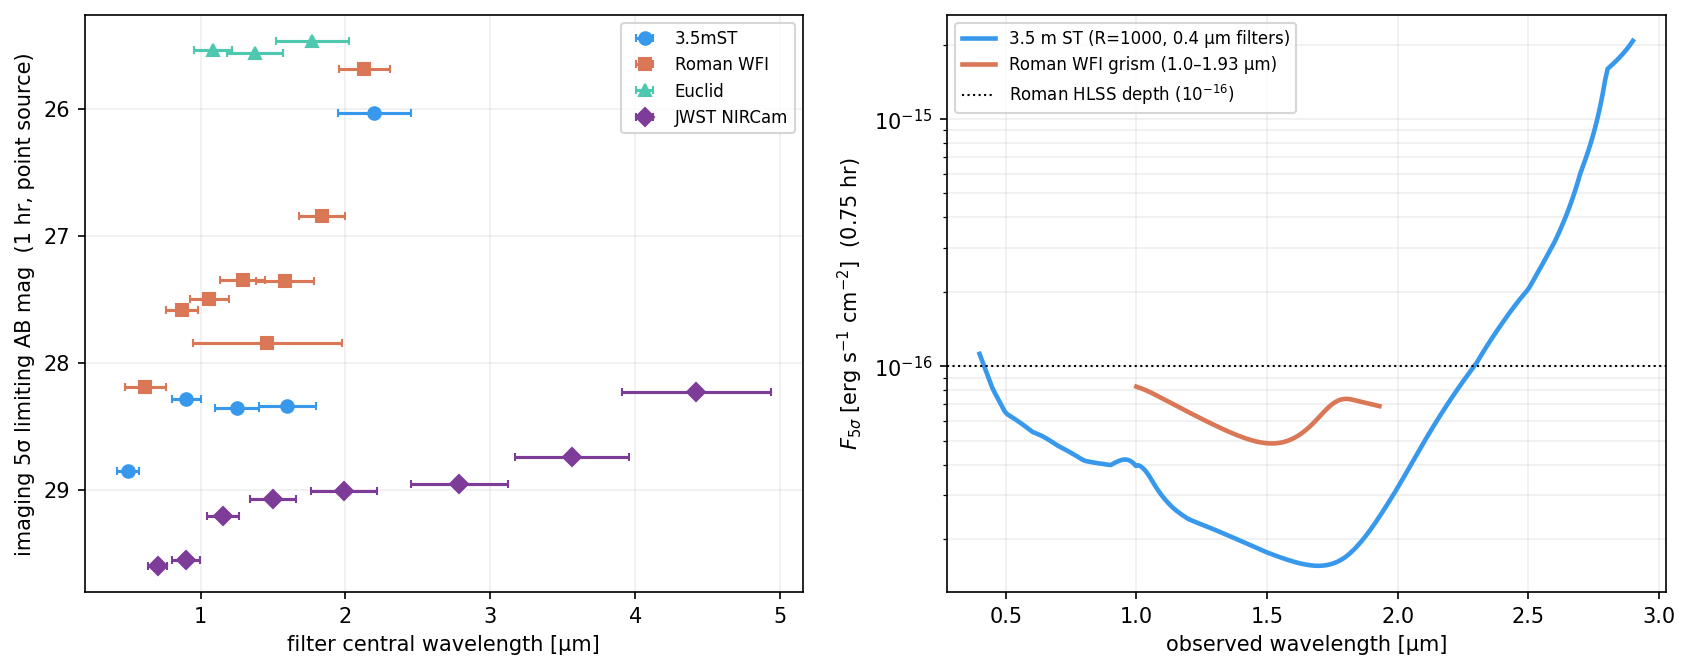
\includegraphics[width=\textwidth]{etc_compare_combined.png}
\caption{\emph{Left}: imaging $5\sigma$ point-source depth in a $1$\,hr exposure, plotted for each mission in its own imaging filters (Roman F062--F213, Euclid Y/J/H, JWST NIRCam F070W--F444W, and representative $3.5$\,m bands). The depth ordering JWST $>$ $3.5$\,m $>$ Roman $>$ Euclid follows collecting area and detector temperature. \emph{Right}: slitless $5\sigma$ line-flux depth versus wavelength in a $0.75$\,hr exposure for the $3.5$\,m concept (band-limiting $0.4\,\mu$m filters, $R=1000$) and the Roman WFI grism, which disperses its full $1.0$--$1.93\,\mu$m band onto each pixel. In the overlap region the $3.5$\,m reaches several times deeper from its larger aperture and its narrower filters, and it also covers the full $0.36$--$3.0\,\mu$m range. The Roman HLSS planning depth is marked.}
\label{fig:compareimg}
\label{fig:comparespec}
\end{figure}

\clearpage
\section{Flagship Survey: ELG BAO and RSD}

\subsection{Science Objective}

The flagship program is a band-limited slitless survey of emission-line galaxies over 100--300 \degti. It will enable us to measure the expansion history through BAO and the growth of structure through RSD, targeting $\fsig(z)$ in broad bins across $1\lesssim z\lesssim3$. The primary tracers are H$\alpha$, [O\,III], H$\beta$, and [O\,II] selected by line flux, color, and direct-image morphology.

The all-line survey target remains of order $10^6$ secure redshifts for a 100 \degti threshold survey and up to a few $10^6$ for a 300 \degti goal survey, but this should not be read as a DESI [O\,II]-only density or as a number that follows from aperture alone. The predicted ELG count is set by the distribution of spectral line strengths and by the redshift-dependent luminosity functions of H$\alpha$, [O\,III], H$\beta$, and [O\,II], folded through the slitless selection function. A direct DESI DR1 \texttt{ELG\_LOPnotqso} calculation gives a conservative [O\,II] anchor of $\simeq3.4\times10^2$ deg$^{-2}$ at $F_{\rm [O\,II]}\ge10^{-16}$ erg s$^{-1}$ cm$^{-2}$ over $0.6<z<1.6$, or $\simeq2.2\times10^2$ deg$^{-2}$ over $1.0<z<1.6$. The wide-tier line-flux threshold of $10^{-16}$\,erg\,s$^{-1}$\,cm$^{-2}$ (Table~\ref{tab:wedding}) is what the headline redshift count above is built on, using the space-based all-line selection (H$\alpha$, [O\,III], H$\beta$, and [O\,II]) rather than a single line. The deeper medium-tier threshold near $5\times10^{-17}$\,erg\,s$^{-1}$\,cm$^{-2}$ is a separate calibration target rather than the count-setting depth, used to validate the redshift selection function and the high-redshift luminosity function against detector-level simulations.

BAO provides a standard ruler through the sound horizon $r_d$. The survey enables us to measure transverse and radial BAO combinations,
\begin{equation}
  \theta_{\rm BAO}(z)\simeq \frac{r_d}{D_M(z)}, \qquad
  \Delta z_{\rm BAO}(z)\simeq \frac{H(z)r_d}{c},
\end{equation}
and therefore to constrain $D_M(z)/r_d$ and $H(z)r_d$. RSD adds the growth observable $\fsig(z)$ from the anisotropic clustering amplitude, where
\begin{equation}
  f(z)\equiv\frac{d\ln D}{d\ln a}
\end{equation}
is the logarithmic growth rate of the linear growth factor $D(a)$ with scale factor $a$. The wide tier drives the BAO/RSD statistical power. The medium and deep tiers calibrate the redshift selection function that otherwise becomes the dominant systematic.

\subsection{Survey Precedent and Redshift Precision}

Roman's High Latitude Spectroscopic Survey provides the closest design precedent. It is a large-area slitless survey with $R\simeq435$--865 that forecasts millions of H$\alpha$ and [O\,III] redshifts and explicitly targets BAO and RSD cosmology \cite{wang2021}. The present design uses native $R=1000$ to retain line-separation margin while keeping spectra short enough for crowded-field deblending. The redshift requirement is not precision internal kinematics. It is a calibrated, high-purity redshift sample with a radial smearing small compared with the BAO scale after quality cuts.

The scale of that precedent is worth stating plainly. Wang et al.'s reference HLSS design covers $2000$\,deg$^2$ to a $10^{-16}\,{\rm erg\,s^{-1}\,cm^{-2}}$, $6.5\sigma$ flux limit, forecasting $\sim10^7$ H$\alpha$ redshifts at $1\lesssim z\lesssim2$ plus $2\times10^6$ [O\,III] redshifts at $2\lesssim z\lesssim3$, with a fractional BAO distance precision of $\sim1$--$2\%$ and a growth-rate precision of $\sim6$--$7\%$ per redshift bin over that range \cite{wang2021}. The present concept's $100$--$300$\,deg$^2$ footprint and $10^6$--$3\times10^6$ redshift range are a fraction of that raw statistical volume. On sample size alone this survey does not exceed what Roman HLSS delivers by itself. Its case rests on three complementary properties instead. It selects on all four lines, H$\alpha$, [O\,III], H$\beta$, and [O\,II], against Roman's own two-line forecast. It runs an independent three-roll deblending pipeline whose systematics are cross-checked against, not shared with, Roman's extraction. Its footprint and cadence are chosen for joint, multi-tracer analysis with Roman, DESI, and HETDEX-class surveys (Section~\ref{sec:anchorsynergy}), where the combined sample and the cross-survey systematics check are the actual statistical gain, rather than for a stand-alone volume that would compete with Roman HLSS on its own.

\begin{leadbox}[title=RSD Survey Definition]{green}
\begin{tabularx}{\textwidth}{@{}p{4.3cm}Y@{}}
\toprule
\textbf{Requirement} & \textbf{Adopted value}\\
\midrule
Field of view & \fovlarge\ required for the wide survey; \fovsmall\ reserved for deep fields and technology validation.\\
Survey area & 100 \degti threshold; 300 \degti goal.\\
Redshift sample & $10^6$ threshold; $3\times10^6$ goal secure ELG redshifts.\\
Spectral mode & $R_{\rm point}=1000$ native, band-limited filters, two dispersion directions.\\
Redshift quality & completeness and purity calibrated as functions of flux, size, line ratio, wavelength, field density, and roll angle.\\
Cosmology target & 3--5\% $\fsig$ precision in broad redshift bins, after end-to-end forecast validation.\\
\bottomrule
\end{tabularx}
\end{leadbox}

\subsection{Representative ELG Spectrum and Detectable Lines}

The target population is a star-forming ELG with blue continuum, nebular recombination lines, and collisionally excited oxygen lines. The most important redshift anchors are [O\,II] $\lambda3727$, H$\beta$ $\lambda4861$, [O\,III] $\lambda4959,\lambda5007$, H$\alpha$ $\lambda6563$, and the neighboring [N\,II]/[S\,II] complex. At native $R=1000$, the [O\,III] doublet is cleanly separated for compact sources over the full cosmological range. H$\alpha$ and [N\,II] are often modeled as a blended complex for extended sources, but still provide a high-S/N redshift feature when combined with morphology priors and other lines.

Table~\ref{tab:lines} translates this line set into the proposed two-arm wavelength coverage, giving the redshift interval over which each diagnostic line falls in the optical and near-IR arms. Its purpose is to show that the redshift solution is normally overconstrained by more than one line across $1<z<3$ rather than depending on a single ambiguous feature.

\begin{figure}[tp]
\centering
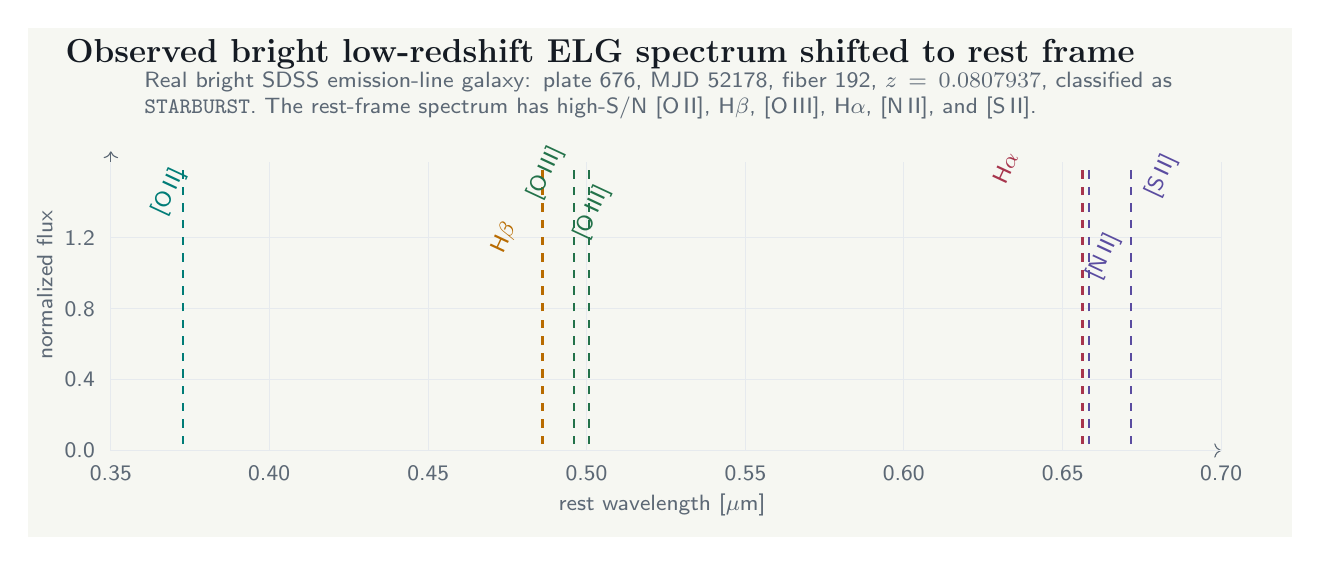
\begin{tikzpicture}[font=\sffamily\footnotesize]
  \fill[paper] (-0.35,-0.35) rectangle (15.7,6.12);
  \node[anchor=west,font=\bfseries\large,color=ink] at (0,5.78) {Observed bright low-redshift ELG spectrum shifted to rest frame};
  \draw[->,color=muted] (0.7,0.75) -- (14.8,0.75);
  \draw[->,color=muted] (0.7,0.75) -- (0.7,4.55);
  \node[anchor=north,color=muted] at (7.7,0.32) {rest wavelength [$\mu$m]};
  \node[rotate=90,anchor=south,color=muted] at (0.08,2.85) {normalized flux};
  \foreach \x/\lab in {0.70/0.35,2.71/0.40,4.73/0.45,6.74/0.50,8.76/0.55,10.77/0.60,12.79/0.65,14.80/0.70} {
    \draw[line!65] (\x,0.75) -- (\x,4.42);
    \node[anchor=north,color=muted] at (\x,0.68) {\lab};
  }
  \foreach \y/\lab in {0.75/0.0,1.65/0.4,2.55/0.8,3.45/1.2} {
    \draw[line!65] (0.7,\y) -- (14.8,\y);
    \node[anchor=east,color=muted] at (0.62,\y) {\lab};
  }
  \begin{scope}[shift={(-13.400,0.82)},x=40.286cm,y=2.28cm]
    \draw[blue,line width=0.72pt] plot file {sdss_elg_rest_spectrum.dat};
  \end{scope}
  \foreach \lam/\lab/\col/\yy/\rot/\dx in {
    0.3727/{[O\,II]}/teal/3.92/65/0.06,
    0.4861/{H$\beta$}/gold/3.34/65/-0.26,
    0.4959/{[O\,III]}/green/4.16/65/-0.12,
    0.5007/{[O\,III]}/green/3.66/65/0.28,
    0.6563/{H$\alpha$}/rose/4.24/65/-0.78,
    0.6584/{[N\,II]}/violet/3.10/65/0.42,
    0.6717/{[S\,II]}/violet/4.12/65/0.62} {
    \pgfmathsetmacro{\xx}{0.7 + (\lam-0.35)*40.286}
    \draw[\col,line width=0.8pt,dashed] (\xx,0.83) -- (\xx,4.36);
    \node[anchor=south,rotate=\rot,color=\col] at (\xx+\dx,\yy) {\lab};
  }
  \node[anchor=west,text width=13.5cm,color=muted] at (1.0,5.26)
  {Real bright SDSS emission-line galaxy: plate 676, MJD 52178, fiber 192, $z=0.0807937$, classified as \texttt{STARBURST}. The rest-frame spectrum has high-S/N [O\,II], H$\beta$, [O\,III], H$\alpha$, [N\,II], and [S\,II].};
\end{tikzpicture}
\caption{Observed bright low-redshift emission-line galaxy spectrum from SDSS DR17. This nearby starburst ELG is used to show the high-S/N line set that anchors slitless redshift identification. The bright lines are [O\,II], H$\beta$, [O\,III], H$\alpha$, [N\,II], and [S\,II]. Data source: SDSS DR17 spectrum spec-0676-52178-0192 \cite{sdssdr17}.}
\label{fig:elgspectrum}
\end{figure}

\begin{table}[tp]
\centering
\sffamily\small
\begin{tabularx}{\textwidth}{@{}p{2.8cm}p{2.1cm}p{2.8cm}p{2.8cm}Y@{}}
\toprule
\textbf{Line} & \textbf{Rest $\lambda$} & \textbf{0.3--1.0 $\mu$m arm} & \textbf{1.0--3.0 $\mu$m arm} & \textbf{Cosmology use}\\
\midrule
{[O\,II]} & 0.3727 $\mu$m & $0<z<1.68$ & $1.68<z<7.05$ & Key line for $z\gtrsim1.7$ when H$\alpha$ leaves the band; doublet/SED priors help purity.\\
H$\beta$ & 0.4861 $\mu$m & $0<z<1.06$ & $1.06<z<5.17$ & Secondary confirmation line with [O\,III].\\
{[O\,III]} & 0.4959, 0.5007 $\mu$m & $0<z<1.00$ & $1.00<z<4.99$ & High-EW workhorse for $1<z<3$; doublet separation aids redshift purity.\\
H$\alpha$ & 0.6563 $\mu$m & $0<z<0.52$ & $0.52<z<3.57$ & Primary low-to-mid-$z$ BAO tracer; strongest line for many star-forming galaxies.\\
{[S\,II]} & 0.6716, 0.6731 $\mu$m & $0<z<0.49$ & $0.49<z<3.47$ & Template support near H$\alpha$; useful for bright calibration spectra.\\
\bottomrule
\end{tabularx}
\caption{Observed redshift windows for the proposed two-arm spectrograph. The ELG BAO core is $1\lesssim z\lesssim3$, where H$\alpha$, [O\,III], and [O\,II] provide overlapping redshift confirmation paths.}
\label{tab:lines}
\end{table}

\begin{figure}[tp]
\centering
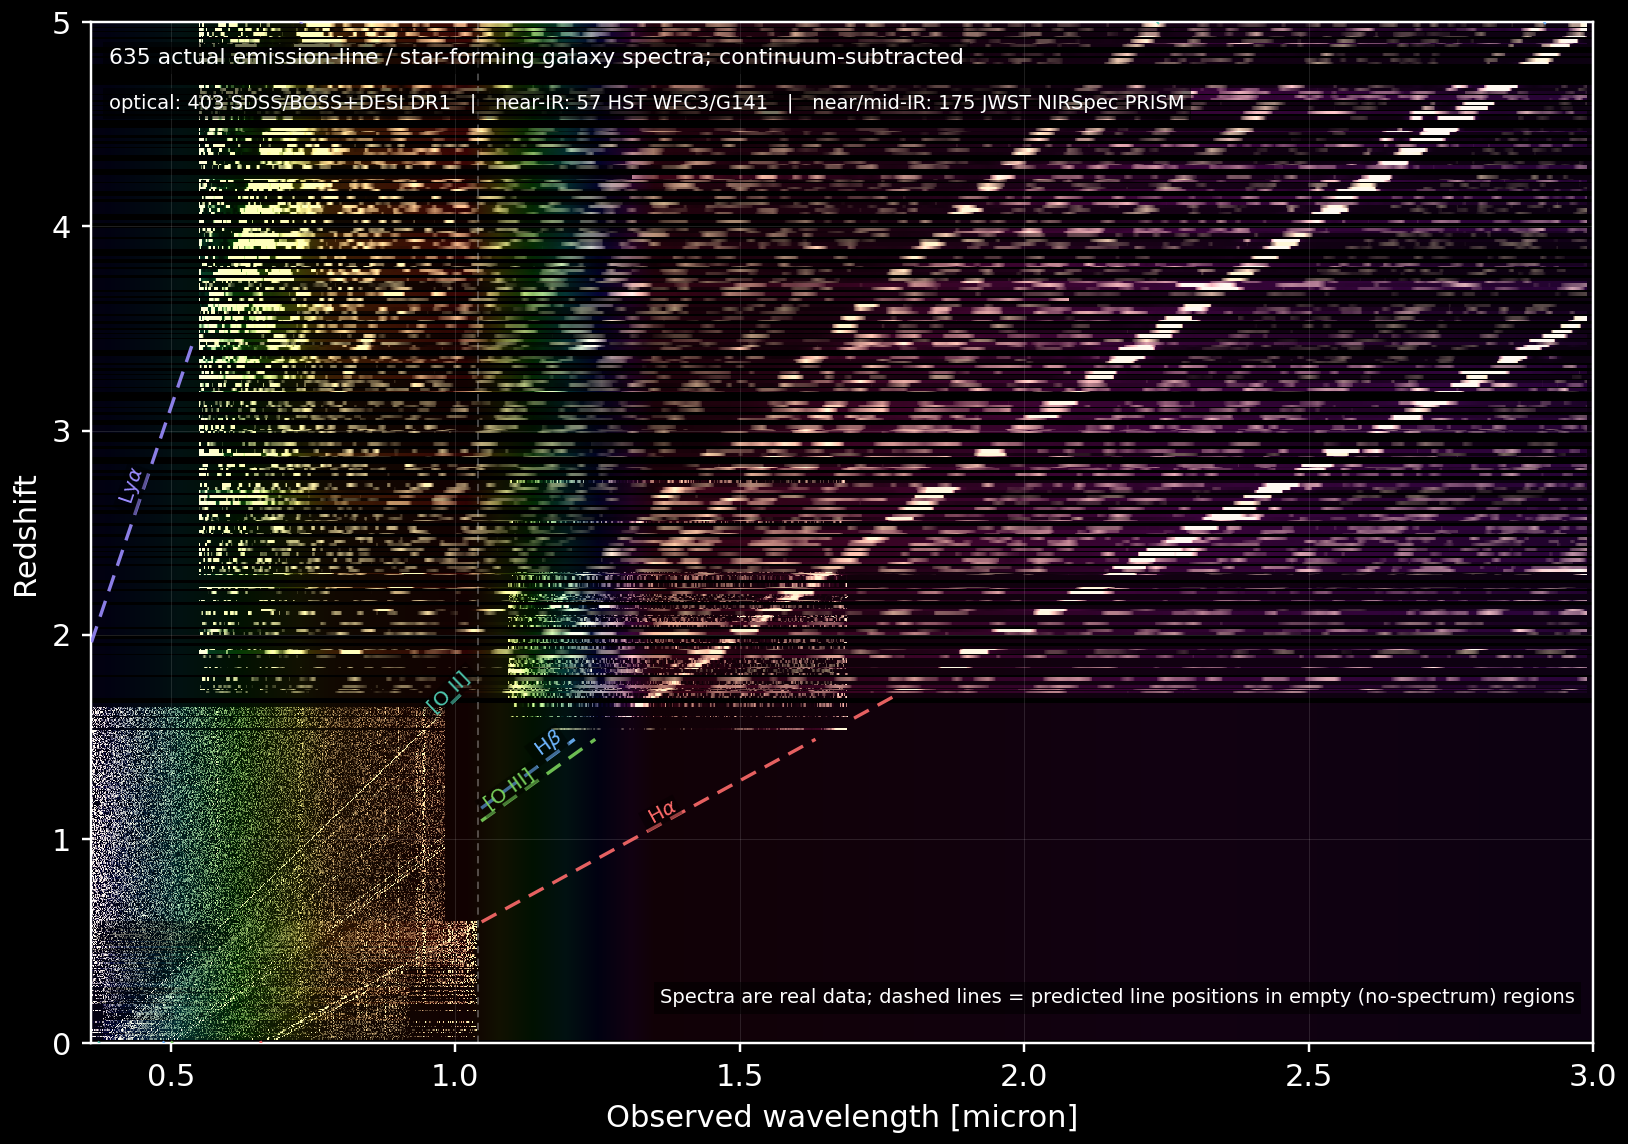
\includegraphics[width=0.98\textwidth,height=0.50\textheight,keepaspectratio]{elg_desi_uniform_actual_2df_style.png}
\caption{Actual ELG/star-forming galaxy spectral stack in observed wavelength and redshift, in the compact ``spectral barcode'' style of the 2dF QSO atlas, spanning the full $0.36$--$3.0\,\mu$m proposed band and $0<z<5$, with the dashed line near $1.04\,\mu$m marking the optical/near-IR arm split. Four real datasets are stacked at their catalog redshifts, 110 SDSS/BOSS and 293 DESI DR1 ELGs ($z\lesssim1.65$, via SPARCL) in the optical arm, 57 HST WFC3/G141 3D-HST COSMOS grism spectra ($1.5<z<2.75$) in the near-IR, and 175 JWST/NIRSpec PRISM star-forming galaxies ($1.7<z<5.0$, DAWN JWST Archive) at high redshift, $635$ spectra in total. Each row is continuum-subtracted and scaled to emphasize line residuals. The continuous diagonal tracks ([O\,II], H$\beta$+[O\,III], H$\alpha$) run unbroken from the optical block through the JWST band, demonstrating that the line set the survey relies on stays observable across $1\lesssim z\lesssim3$ and beyond. No spectra are synthetic. Dashed labelled lines trace the predicted $\lambda_{\rm obs}=\lambda_{\rm rest}(1+z)$ track of each diagnostic line only in the empty, no-data regions, never overplotting real data \cite{raichoor2022,desidr1,sparcl2024,brammer2012,momcheva2016,degraaff2024,heintz2023}.}
\label{fig:elgobswavez}
\end{figure}

\subsection{ELG Luminosity, Distance, and Depth}\label{sec:elgdepth}

The planning model uses a flat $\Lambda$CDM cosmology with $H_0=70$ km s$^{-1}$ Mpc$^{-1}$ and $\Omega_m=0.3$. For continuum magnitude estimates,
\begin{equation}
  m_{\rm AB}=M_{\rm AB}+\mu(z)+K(z), \qquad
  \mu(z)=5\log_{10}\!\left[\frac{D_L(z)}{\rm Mpc}\right]+25,
\end{equation}
where $K(z)$ is the bandpass-dependent $K$-correction. For emission-line selection,
\begin{equation}
  F_{\rm line}=\frac{L_{\rm line}}{4\pi D_L^2}.
\end{equation}
Representative star-forming ELGs at $1<z<3$ occupy roughly $M_{\rm AB}\simeq-19$ to $-22.5$, with the highest-yield BAO sample concentrated near $M_{\rm AB}\simeq-20.5$ to $-21.5$ and line luminosities $L_{\rm H\alpha}$ or $L_{\rm [O\,III]}\sim10^{42}$--$10^{43}$ erg s$^{-1}$. Table~\ref{tab:elgdepth} gives planning values before detailed luminosity-function integration and ETC validation. It is meant to connect absolute magnitude, observed continuum magnitude, emission-line flux, and (on the same redshift grid) the tier-by-tier line-luminosity depth derived in Eq.~\eqref{eq:f5sigma} below.

\begin{table}[tp]
\centering
\sffamily\small
\setlength{\tabcolsep}{4.5pt}
\begin{tabularx}{\textwidth}{@{}c c c c c c !{\hskip 8pt} c c c@{}}
\toprule
& & & & & & \multicolumn{3}{c@{}}{\textbf{Line-luminosity limit $L_{5\sigma}$ [erg s$^{-1}$]}}\\
\cmidrule(l){7-9}
\textbf{$z$} & \textbf{$\mu(z)$} & \textbf{$m(M=-20)$} & \textbf{$m(M=-21)$} & \textbf{$F(10^{42})$} & \textbf{$F(3\times10^{42})$} & \textbf{Wide} & \textbf{Medium} & \textbf{Deep}\\
 & mag & mag & mag & erg s$^{-1}$ cm$^{-2}$ & erg s$^{-1}$ cm$^{-2}$ & & &\\
\midrule
1.0 & 44.10 & 24.1 & 23.1 & $1.9\times10^{-16}$ & $5.7\times10^{-16}$ & $5.2\times10^{41}$ & $2.6\times10^{41}$ & $1.3\times10^{41}$\\
1.5 & 45.19 & 25.2 & 24.2 & $7.0\times10^{-17}$ & $2.1\times10^{-16}$ & $1.4\times10^{42}$ & $7.1\times10^{41}$ & $3.6\times10^{41}$\\
2.0 & 45.96 & 26.0 & 25.0 & $3.5\times10^{-17}$ & $1.0\times10^{-16}$ & $2.9\times10^{42}$ & $1.4\times10^{42}$ & $7.2\times10^{41}$\\
2.5 & 46.55 & 26.5 & 25.5 & $2.0\times10^{-17}$ & $6.0\times10^{-17}$ & $5.0\times10^{42}$ & $2.5\times10^{42}$ & $1.2\times10^{42}$\\
3.0 & 47.03 & 27.0 & 26.0 & $1.3\times10^{-17}$ & $3.9\times10^{-17}$ & $7.8\times10^{42}$ & $3.9\times10^{42}$ & $1.9\times10^{42}$\\
\bottomrule
\end{tabularx}
\caption{Left: planning relation between ELG absolute magnitude, apparent magnitude, and line flux, on the same redshift grid as the flux-to-luminosity conversion. Continuum magnitudes omit $K(z)$, which is typically of order several tenths to one magnitude depending on rest-frame wavelength and galaxy SED. Right: the line-luminosity limit $L_{5\sigma}$ implied by the wide, medium, and deep planning flux depths (Eq.~\eqref{eq:f5sigma}). A $3\times10^{42}$ erg s$^{-1}$ ELG is a wide-tier object to $z\simeq2$, a medium-tier object to $z\simeq2.5$, and a deep-tier object beyond $z\simeq3$ depending on line identity and background.}
\label{tab:elgdepth}
\label{tab:llumlim}
\end{table}

For survey planning, the line-flux limit is parameterized as
\begin{equation}
  F_{5\sigma}(t_{\rm tot})\simeq
  1.0\times10^{-16}
  \left(\frac{0.75\ {\rm hr}}{t_{\rm tot}}\right)^{1/2}
  {\rm erg\ s^{-1}\ cm^{-2}},
  \label{eq:f5sigma}
\end{equation}
where $t_{\rm tot}$ is the summed spectroscopic exposure over the required three orientations in a given band. The $t_{\rm tot}^{-1/2}$ dependence is the background-limited (sky-dominated) scaling. For a faint line integrated over a fixed number of resolution-element pixels, the accumulated sky background grows as $t_{\rm tot}$ and its Poisson shot noise as $t_{\rm tot}^{1/2}$ while the line signal grows as $t_{\rm tot}$. Therefore, ${\rm S/N}\propto t_{\rm tot}^{1/2}$ at fixed flux and hence $F_{5\sigma}\propto t_{\rm tot}^{-1/2}$. By definition $F_{5\sigma}$ is the line flux whose integrated signal equals five times this sky-background-dominated noise (a $5\sigma$ detection). Detector read noise and the source's own shot noise are subdominant at this depth. The normalization, $1.0\times10^{-16}\,{\rm erg\,s^{-1}\,cm^{-2}}$ at $t_{\rm tot}=0.75$ hr, is anchored to the published $5$--$6.5\sigma$ line-flux limits of comparable space slitless-grism surveys (Roman HLSS and Euclid) rather than to a detector-level ETC \cite{wang2021,euclid2011}. It implies $F_{5\sigma}\simeq1.0\times10^{-16}$, $5\times10^{-17}$, and $2.5\times10^{-17}\,{\rm erg\,s^{-1}\,cm^{-2}}$ at $t_{\rm tot}=0.75$, 3, and 12 hr respectively. Using $L_{\rm line}=4\pi D_L^2 F_{5\sigma}$ with $D_L(z=2)\simeq15.5$ Gpc for the adopted flat $\Lambda$CDM cosmology, these correspond at $z\simeq2$ to $L_{\rm line}\simeq2.9\times10^{42}$, $1.4\times10^{42}$, and $7\times10^{41}$ erg s$^{-1}$, respectively. The instrument sensitivity underlying this normalization, with its cross-checks against Roman, Euclid, and JWST, is derived in Section~\ref{sec:etc}.

For an isolated line, the planning signal-to-noise ratio is
\begin{equation}
  {\rm S/N}_{\rm line}\simeq 5\,\frac{F_{\rm line}}{F_{5\sigma}(t_{\rm tot})}\,C_{\rm blend},
  \label{eq:snline}
\end{equation}
where $C_{\rm blend}\simeq0.7$--1 represents loss from morphology, background, and residual overlap after the three-orientation deblending fit. Table~\ref{tab:snrelg} gives the pre-blending S/N, i.e. the values for $C_{\rm blend}=1$. Object-level S/N values should be reduced by the fitted $C_{\rm blend}$ and by the catalog covariance model.

\begin{table}[tp]
\centering
\sffamily\small
\begin{tabularx}{\textwidth}{@{}p{2.3cm}p{3.3cm}c c c c@{}}
\toprule
 & & \multicolumn{4}{c}{\textbf{Approximate emission-line S/N}}\\
\cmidrule(lr){3-6}
\textbf{Tier} & \textbf{$F_{5\sigma}$ \ (exposure $t_{\rm tot}$)} & \multicolumn{4}{c}{at line flux $F$ [erg s$^{-1}$ cm$^{-2}$]:}\\
 & [erg s$^{-1}$ cm$^{-2}$] & $3\times10^{-17}$ & $10^{-16}$ & $3\times10^{-16}$ & $10^{-15}$\\
\midrule
Wide & $1.0\times10^{-16}$ \ (0.75 hr) & 1.5 & 5 & 15 & 50\\
Medium & $5.0\times10^{-17}$ \ (3 hr) & 3 & 10 & 30 & 100\\
Deep pencil & $2.5\times10^{-17}$ \ (12 hr) & 6 & 20 & 60 & 200\\
Ultra-deep & $1.3\times10^{-17}$ \ (48 hr) & 12 & 38 & 115 & 385\\
\bottomrule
\end{tabularx}
\caption{Approximate emission-line S/N before applying the object-specific blending/morphology factor. The second column lists, for each survey tier, the line-flux depth $F_{5\sigma}$ together (in parentheses) with the corresponding single-region total exposure time $t_{\rm tot}$, i.e. the three-orientation summed science exposure per band, related by $F_{5\sigma}\propto t_{\rm tot}^{-1/2}$ and matching the tiers of Table~\ref{tab:wedding}. All line fluxes ($F_{5\sigma}$ and the $F$ values in the column headers) are in erg s$^{-1}$ cm$^{-2}$. Secure cosmology redshifts require either S/N $\gtrsim7$--10 in a single line with strong priors, or multi-line/template confirmation at lower individual-line S/N.}
\label{tab:snrelg}
\end{table}

Table~\ref{tab:llumlim} (right side) gives the same depth model in luminosity rather than flux. Each entry is the line luminosity that would be detected at S/N=5 before the object-specific blending/morphology correction. For any source with luminosity $L_{\rm line}$ at that redshift, the corresponding planning S/N is approximately
\begin{equation}
  {\rm S/N}_{\rm line}\simeq
  5\,\frac{L_{\rm line}}{L_{5\sigma}(z,t_{\rm tot})}\,C_{\rm blend}.
\end{equation}
Thus a source equal to a Table~\ref{tab:llumlim} entry has S/N$\simeq5$ for $C_{\rm blend}=1$ and S/N$\simeq3.5$--5 for the nominal $C_{\rm blend}=0.7$--1 range. A source twice as luminous has twice those S/N values.

\subsubsection{Line-Luminosity-Function Count Model}

The conversion from survey depth to an expected ELG catalog size requires an explicit line-luminosity-function model. For a line $i$ with rest wavelength $\lambda_i$ and luminosity function $\Phi_i(L,z)$, the 5$\sigma$ flux limit gives a redshift-dependent luminosity threshold
\begin{equation}
  L_{{\rm lim},i}(z)=4\pi D_L^2(z)F_{{\rm lim},i}(z),
\end{equation}
modified in practice by throughput, background, morphology, blending, and wavelength-dependent contamination. The differential flux distribution entering the exposure-time calculation is
\begin{equation}
  \frac{d^2N_i}{dF\,dz\,d\Omega}
  =
  4\pi D_L^2(z)\,
  \Phi_i\!\left(4\pi D_L^2F,z\right)
  \frac{dV_c}{dz\,d\Omega},
\end{equation}
where $\Phi_i$ is defined per unit luminosity. If the LF is written per dex in luminosity, the equivalent expression includes the usual factor $d\log L/dF=(F\ln10)^{-1}$. Thus the count forecast is not just an ETC depth calculation. It is the integral of the observed line-strength distribution above the detection threshold in each redshift slice.

For analytic planning the line LF can be represented by a Schechter form \cite{schechter1976,saito2020,mehta2015},
\begin{equation}
  \Phi_i(L,z)dL =
  \phi_i^\star(z)
  \left(\frac{L}{L_i^\star(z)}\right)^{\alpha_i(z)}
  \exp\!\left[-\frac{L}{L_i^\star(z)}\right]
  \frac{dL}{L_i^\star(z)} ,
\end{equation}
where the redshift evolution is part of the model, not a post-processing correction. A convenient planning parameterization is
\begin{equation}
  \begin{aligned}
  \log_{10}L_i^\star(z) &=
  \log_{10}L_{i,0}^\star+
  Q_{L,i}\log_{10}\!\left(\frac{1+z}{1+z_0}\right),\\
  \log_{10}\phi_i^\star(z) &=
  \log_{10}\phi_{i,0}^\star+
  Q_{\phi,i}\log_{10}\!\left(\frac{1+z}{1+z_0}\right),\\
  \alpha_i(z) &= \alpha_{i,0}+Q_{\alpha,i}(z-z_0),
  \end{aligned}
  \label{eq:lf_evolution_planning}
\end{equation}
with separate coefficients for H$\alpha$, [O\,III], H$\beta$, and [O\,II]. Eq.~\eqref{eq:lf_evolution_planning} is a planning interpolation of the redshift-evolving Schechter LF fits in Saito et al. \cite{saito2020} and the single-bin WISP [O\,III] LF fits in Mehta et al. \cite{mehta2015}. For the Saito et al. H$\alpha$ and [O\,II] rows in Table~\ref{tab:lfparams_eq16}, one may set $z_0=0$, $Q_{L,i}=\beta$, $Q_{\alpha,i}=0$, and $Q_{\phi,i}=\gamma$ below $z_{\rm pivot}$, while above $z_{\rm pivot}$ the source model uses the broken normalization slope $Q_{\phi,i}=-\epsilon$ with the continuity factor shown below \cite{saito2020}. In practice these parameters should be fitted in redshift bins with smooth evolution used only to interpolate between calibrated bins. The line flux distribution measured by the survey is then a direct projection of this evolving LF,
\begin{equation}
  \frac{d^2N_i}{dz\,d\Omega}(>F_{\rm lim}) =
  \frac{dV_c}{dz\,d\Omega}
  \int_{4\pi D_L^2(z)F_{\rm lim}}^\infty
  \Phi_i(L,z)\,C_i(L,z)\,dL ,
\end{equation}
where $C_i(L,z)$ is the completeness function of line $i$, the probability between zero and one that a galaxy of line luminosity $L$ at redshift $z$ yields a secure detection of that line in the survey data. In the ideal case $C_i=1$ the line-selected surface density in a redshift bin reduces to the standard luminosity-function projection over comoving volume \cite{schechter1976,saito2020,mehta2015},
\begin{equation}
  \Sigma_i(z_1,z_2;F_{\rm lim}) =
  \int_{z_1}^{z_2}
  \frac{dV_c}{dz\,d\Omega}
  \int_{L_{{\rm lim},i}(z)}^\infty
  \Phi_i(L,z)\,dL\,dz .
  \label{eq:lf_surface_density}
\end{equation}
Equivalently, for a pure Schechter LF this inner integral is $\phi_i^\star\Gamma(\alpha_i+1,L_{\rm lim}/L_i^\star)$, but numerical integration is preferred because ELG faint-end slopes, LF evolution, and completeness functions are not perfectly described by a single Schechter law.
Table~\ref{tab:lfparams_eq16} lists the explicit literature parameter values adopted as starting inputs for Eq.~\eqref{eq:lf_evolution_planning} and for the Eq.~\eqref{eq:lf_surface_density} surface-density integral. Saito et al. use
$L^\star(z)=L^\star_{*,0}(1+z)^\beta$ and
$\Phi^\star(z)=\Phi^\star_{*,0}(1+z)^\gamma$ below $z_{\rm pivot}$, with
$\Phi^\star(z)=\Phi^\star_{*,0}(1+z_{\rm pivot})^{\gamma+\epsilon}(1+z)^{-\epsilon}$ above $z_{\rm pivot}$ \cite{saito2020}. H$\beta$ is not assigned an independent LF in this planning table. It is propagated as a secondary confirmation line through the line-ratio model, e.g. H$\alpha$/H$\beta=2.9$ and [O\,III]/H$\beta=4.1$ in the Saito et al. nebular-line prescription \cite{saito2020}.

\begin{table}[tp]
\centering
\sffamily\scriptsize
\begin{tabularx}{\textwidth}{@{}p{1.7cm}p{1.9cm}c c c c c c Y@{}}
\toprule
\textbf{Line} & \textbf{$z$ range} & \textbf{$\log_{10}\Phi^\star_{*,0}$} & \textbf{$\gamma$} & \textbf{$\epsilon$} & \textbf{$z_{\rm pivot}$} & \textbf{$\log_{10}L^\star_{*,0}$} & \textbf{$\alpha$} & \textbf{Source / note}\\
 & & Mpc$^{-3}$ & & & & erg s$^{-1}$ & & \\
\midrule
H$\alpha$ & $0.3<z<2.0$ & $-2.92\pm0.03$ & $1.30\pm0.12$ & $1.86\pm1.40$ & $1.53\pm0.12$ & $41.59\pm0.03$ & $-1.35$ & Saito et al.; also $\beta=1.91\pm0.08$.\\
{[O\,II]} & $0.3<z<2.5$ & $-1.89\pm0.04$ & $-1.96\pm0.18$ & $-2.48\pm0.21$ & $1.00\pm0.02$ & $40.73\pm0.02$ & $-1.25$ & Saito et al.; also $\beta=2.61\pm0.08$.\\
{[O\,III]} & $0.8<z<1.2$ & $-3.17^{+0.27}_{-0.39}$ & \multicolumn{3}{c}{single-bin Schechter LF} & $42.21^{+0.22}_{-0.18}$ & $-1.42^{+0.23}_{-0.43}$ & Mehta et al. WISP [O\,III] LF.\\
{[O\,III]} & $1.85<z<2.2$ & $-2.69^{+0.31}_{-0.51}$ & \multicolumn{3}{c}{single-bin Schechter LF} & $42.55^{+0.28}_{-0.19}$ & $-1.57^{+0.28}_{-0.77}$ & Mehta et al. WISP [O\,III] LF.\\
\bottomrule
\end{tabularx}
\caption{Literature LF parameter values to use with the Eq.~\eqref{eq:lf_evolution_planning} redshift-evolution parameterization and the Eq.~\eqref{eq:lf_surface_density} surface-density integral. Values are starting points for exposure-time and number-count forecasts. The mission forecast must refit them with its own medium/deep calibration tiers and include completeness $C_i(L,z)$.}
\label{tab:lfparams_eq16}
\end{table}

The secure-redshift catalog is the union of several line selections, not the sum of independent H$\alpha$, [O\,III], H$\beta$, and [O\,II] counts. A practical forecast should integrate over galaxy properties $\boldsymbol{\theta}$ such as line ratios, equivalent widths, continuum magnitude, half-light radius, dust attenuation, and local spectral crowding:
\begin{equation}
  N_{\rm secure} =
  \Omega_{\rm surv}
  \int dz\,\frac{dV_c}{dz\,d\Omega}
  \int d\boldsymbol{\theta}\,
  n(\boldsymbol{\theta}|z)\,
  P_{\rm secure}(\boldsymbol{\theta},z).
\end{equation}
Here $n(\boldsymbol{\theta}|z)$ is the comoving number density of galaxies per unit property interval at redshift $z$. It is the multivariate generalization of the luminosity function of Eq.~\eqref{eq:lf_surface_density}, in which the single luminosity is replaced by the full property vector $\boldsymbol{\theta}$. It is normalized so that $\int d\boldsymbol{\theta}\,n(\boldsymbol{\theta}|z)$ recovers the total comoving number density at $z$. The factor $P_{\rm secure}(\boldsymbol{\theta},z)$ lies between zero and one. It is the redshift-success probability, the fraction of galaxies with those properties for which the pipeline returns a cosmology-grade redshift. It is given explicitly below. The expression is a selection-weighted population count rather than a Bayesian inference. The conditional notation $(\,\cdot\,|z)$ denotes evaluation at redshift $z$ rather than a posterior. The redshift-success probability is approximately
\begin{equation}
  P_{\rm secure}=1-\prod_i
  \left[1-C_i(F_i,z,\boldsymbol{\theta})\right],
\end{equation}
with the important caveat that the $C_i$ are correlated because the same galaxy supplies multiple lines. In slitless data $C_i$ must include line S/N, continuum priors from the direct image, source size relative to the dispersion direction, roll-angle overlap probability, line confusion, and the probability that a single-line solution is accepted as cosmology grade. This is why the medium and deep tiers are not optional depth demonstrations. They enable us to measure the LF tails, line-ratio distribution, and incompleteness needed to transfer the wide-tier target density into an unbiased clustering selection function.

The minimum LF calibration set for this mission is therefore:
\begin{itemize}
  \item H$\alpha$ LF over $0.5\lesssim z\lesssim3.5$, because H$\alpha$ is the strongest line for many star-forming galaxies, anchoring the low-to-mid redshift BAO sample.
  \item [O\,III] and H$\beta$ LFs over $1\lesssim z\lesssim3$, because high-equivalent-width [O\,III] emitters dominate part of the near-IR selection, providing strong multi-line confirmation.
  \item [O\,II] LF over $1\lesssim z\lesssim3$, because [O\,II] remains in band after H$\alpha$ shifts toward the long-wavelength edge, supplying continuity with DESI/eBOSS.
  \item Joint distributions of line ratios, equivalent width, dust, size, and continuum magnitude, because the probability of detecting at least one secure redshift feature depends on correlated galaxy properties, not on four independent one-line LFs.
\end{itemize}
The DESI-derived [O\,II] calculation below is therefore used only as a low-redshift empirical anchor. The full 3.5 m all-line survey yield must be derived from a redshift-dependent LF plus selection-function model, then validated with image-level simulations and deeper calibration fields.

\subsubsection{DESI [O\,II] Luminosity-Function Anchor}

The first redshift-dependent number-count estimate is derived directly from the local DESI DR1 LSS \texttt{ELG\_\allowbreak LOPnotqso} FITS table rather than from a fitted analytic Schechter function. DESI ELG target selection and validation show that the Main ELG sample is selected by a $g$-band cut plus a $(g-r)$--$(r-z)$ color box, with two disjoint subsamples of about 1940 and 460 targets deg$^{-2}$, and that reliable ELG redshifts are assessed using [O\,II] flux information \cite{raichoor2022}. We therefore set the effective area of the downloaded table by
\begin{equation}
  \Omega_{\rm eff}=
  \frac{N_{\rm target}}{2400\ {\rm deg}^{-2}}
  =
  \frac{971427}{2400}
  \simeq405\ {\rm deg}^{2},
\end{equation}
and select secure [O\,II] galaxies with \texttt{ZWARN=0}, finite positive redshift, positive \texttt{OII\_FLUX}, and
\begin{equation}
  {\rm S/N}_{\rm [O\,II]}=
  {\tt OII\_FLUX}\,({\tt OII\_FLUX\_IVAR})^{1/2}>5 .
\end{equation}
The line luminosity is computed as
\begin{equation}
  L_{\rm [O\,II]}=4\pi D_L^2(z)F_{\rm [O\,II]},
\end{equation}
using the same flat $\Lambda$CDM cosmology as the rest of this section. In a redshift bin $z_1<z<z_2$, the binned observed luminosity function is
\begin{equation}
  \widehat{\Phi}(\log L_k,z_j)=
  \frac{N_k}
  {\Omega_{\rm eff}\,V_{\rm c,deg^2}(z_1,z_2)\,\Delta\log L\,\overline{C}_k},
\end{equation}
where $V_{\rm c,deg^2}$ is the comoving volume per square degree in the redshift bin and $\overline{C}_k$ is the mean completeness correction in luminosity bin $k$. The conservative DESI table below sets $\overline{C}_k=1$. Therefore, the medium-depth counts should be read as lower limits rather than as a complete faint-end extrapolation. For an observed LF table, the predicted count distribution in one field of view is computed by summing the measured LF bins above the luminosity threshold,
\begin{equation}
  \Delta N_{{\rm FOV},j}(>F_{\rm lim}) =
  A_{\rm FOV}\,
  V_{\rm c,deg^2}(z_j)
  \sum_{\log L_k>\log L_{\rm lim}(z_j)}
  \widehat{\Phi}(\log L_k,z_j)\,
  \Delta\log L\,
  \overline{P}_{{\rm secure},k,j},
\end{equation}
with $A_{\rm FOV}=0.25$ deg$^2$ for one \fovlarge\ frame. This is the explicit step that takes an observed LF and returns the number of galaxies expected in one pointing. The observable surface density for a survey flux limit $F_{\rm lim}$ is then equivalently
\begin{equation}
  \Sigma(>F_{\rm lim},z_1,z_2)=
  \int_{\log L_{\rm lim}}^\infty
  \widehat{\Phi}(\log L,z)\,V_{\rm c,deg^2}\,d\log L
  =
  \frac{N(F_{\rm [O\,II]}>F_{\rm lim})}{\Omega_{\rm eff}},
\end{equation}
with $L_{\rm lim}=4\pi D_L^2(z_{\rm mid})F_{\rm lim}$. A single \fovlarge\ frame has area 0.25 deg$^2$ and, therefore, $N_{\rm frame}=0.25\Sigma$. Table~\ref{tab:desiLFcounts} summarizes this DESI-derived anchor. It uses DESI [O\,II] only. Therefore, it is a conservative anchor for the proposed all-line slitless survey, not the full H$\alpha$+[O\,III]+[O\,II] yield. For $z>1.6$, DESI no longer provides the same direct [O\,II] calibration. Hence, the high-redshift extension must be tied to external [O\,II]/H$\alpha$ luminosity-function and number-count measurements \cite{comparat2015,saito2020,mehta2015}.

\begin{table}[tp]
\centering
\sffamily\scriptsize
\begin{tabularx}{\textwidth}{@{}c c c c c c c@{}}
\toprule
\textbf{$z$ bin} & \textbf{$\log L_{\rm lim,wide}$} & \textbf{$n_{\rm DESI}$} & \textbf{$\Sigma_{\rm wide}$} & \textbf{$\Sigma_{\rm med}$} & \textbf{$N_{\rm frame,wide}$} & \textbf{$N_{\rm frame,med}$}\\
 & $\log_{10}({\rm erg\ s}^{-1})$ & $10^{-5}$ Mpc$^{-3}$ & deg$^{-2}$ & deg$^{-2}$ & ELGs per 0.25 deg$^2$ & ELGs per 0.25 deg$^2$\\
 & $F_{\rm lim}=10^{-16}$ & $>L_{\rm lim,wide}$ & $F_{\rm lim}=10^{-16}$ & $F_{\rm lim}=5\times10^{-17}$ & $F_{\rm lim}=10^{-16}$ & $F_{\rm lim}=5\times10^{-17}$\\
\midrule
0.6--0.8 & 41.34 & 2.34 & 25.9 & 35.4 & 6.5 & 8.8\\
0.8--1.0 & 41.60 & 6.47 & 94.6 & 118.4 & 23.6 & 29.6\\
1.0--1.2 & 41.82 & 5.35 & 93.6 & 119.2 & 23.4 & 29.8\\
1.2--1.4 & 42.00 & 3.95 & 77.9 & 104.7 & 19.5 & 26.2\\
1.4--1.6 & 42.15 & 2.45 & 52.4 & 69.4 & 13.1 & 17.4\\
\bottomrule
\end{tabularx}
\caption{DESI-derived [O\,II] number-count anchor by redshift. The table is computed from the local DESI DR1 \texttt{ELG\_LOPnotqso} catalog using \texttt{ZWARN=0} and [O\,II] S/N$>5$. The effective area is inferred from the DESI Main ELG target density, $1940+460\simeq2400$ deg$^{-2}$, and the 971,427 targets in the local table \cite{raichoor2022}. The quoted $n_{\rm DESI}$ is the integrated observed number density above the wide-tier luminosity limit, not a Schechter-fit $\phi^\star$. Medium counts are lower limits for a truly deeper survey because the DESI target catalog is not complete at arbitrarily faint [O\,II] flux.}
\label{tab:desiLFcounts}
\end{table}

Summing the observed-LF redshift bins in Table~\ref{tab:desiLFcounts} gives the expected [O\,II]-only count per \fovlarge\ pointing shown in Table~\ref{tab:desiFOVsum}. These values are not the final all-line ELG yield. They are a conservative empirical floor showing how the measured DESI [O\,II] LF maps into one 0.25 deg$^2$ field for the adopted flux thresholds.

\begin{table}[tp]
\centering
\sffamily\small
\begin{tabularx}{\textwidth}{@{}c c c c c@{}}
\toprule
\textbf{Redshift range} & \textbf{$\Sigma_{\rm wide}$} & \textbf{$N_{\rm FOV,wide}$} & \textbf{$\Sigma_{\rm med}$} & \textbf{$N_{\rm FOV,med}$}\\
 & deg$^{-2}$ & ELGs per 0.25 deg$^2$ & deg$^{-2}$ & ELGs per 0.25 deg$^2$\\
\midrule
0.6--1.0 & 120.5 & 30.1 & 153.8 & 38.5\\
1.0--1.6 & 223.9 & 56.0 & 293.3 & 73.3\\
0.6--1.6 & 344.4 & 86.1 & 447.1 & 111.8\\
\bottomrule
\end{tabularx}
\caption{Cumulative field-of-view counts obtained by inserting the observed DESI [O\,II] LF into the FOV count equation. The wide threshold is $F_{\rm lim}=10^{-16}$ erg s$^{-1}$ cm$^{-2}$ and the medium threshold is $F_{\rm lim}=5\times10^{-17}$ erg s$^{-1}$ cm$^{-2}$. The all-line space-survey count should be larger only if H$\alpha$, [O\,III], H$\beta$, and high-redshift [O\,II] LFs plus the slitless redshift-success model support that increase.}
\label{tab:desiFOVsum}
\end{table}

The corresponding continuum planning depths, for binned low-resolution spectral elements or matched direct imaging used as extraction priors, are approximately
\begin{equation}
  m_{\rm lim}(t_{\rm tot})\simeq24.3+
  1.25\log_{10}\!\left(\frac{t_{\rm tot}}{0.75\ {\rm hr}}\right).
\end{equation}
This gives $m_{\rm AB}\simeq24.3$, 25.1, 25.8, and 26.6 mag for $t_{\rm tot}=0.75$, 3, 12, and 48 hr, respectively. The line-selected ELG catalog is therefore deeper in star-formation activity than in continuum mass completeness, which is why the medium and deep tiers are needed to calibrate selection.

Figure~\ref{fig:elgmagdepth} places these continuum limits on an observed ELG catalog. We use the DESI DR1 LSS \texttt{ELG\_LOPnotqso} full catalog, select galaxy spectra with \texttt{ZWARN=0} and [O\,II] signal-to-noise greater than 5, and compute an observed-frame $r$-band magnitude from the Legacy Surveys fluxes,
\begin{equation}
  M_r-5\log_{10}h
  =
  m_r-
  \left[
  5\log_{10}\!\left(\frac{D_L}{h^{-1}{\rm Mpc}}\right)+25
  \right],
\end{equation}
without applying a $K$-correction. The black curve marks the effective eBOSS $r$-band limit, $r\simeq22.44$, retained only as a historical comparison line. The purple curve marks the DESI DR1 99th-percentile depth of the plotted secure ELG sample, $r\simeq24.08$. The DESI target selection is not a pure $r$-band cut. It uses a $g$-band magnitude cut and a $(g-r)$ versus $(r-z)$ color box. Therefore, the plotted depth curves should be read as observed-frame indicators of catalog truncation rather than formal single-band selection boundaries \cite{raichoor2022}. The plotted catalog points are clipped at the adopted wide-tier continuum limit, $m_r\le24.3$. Hence, galaxies fainter than the nominal target limit are not shown. DESI occupies the key $0.6<z<1.6$ range and reaches nearly the proposed wide-tier continuum depth. The proposed space survey extends this selection logic to $1\lesssim z\lesssim3$ using deeper medium/deep tiers and near-infrared emission lines.

\begin{figure}[tp]
\centering
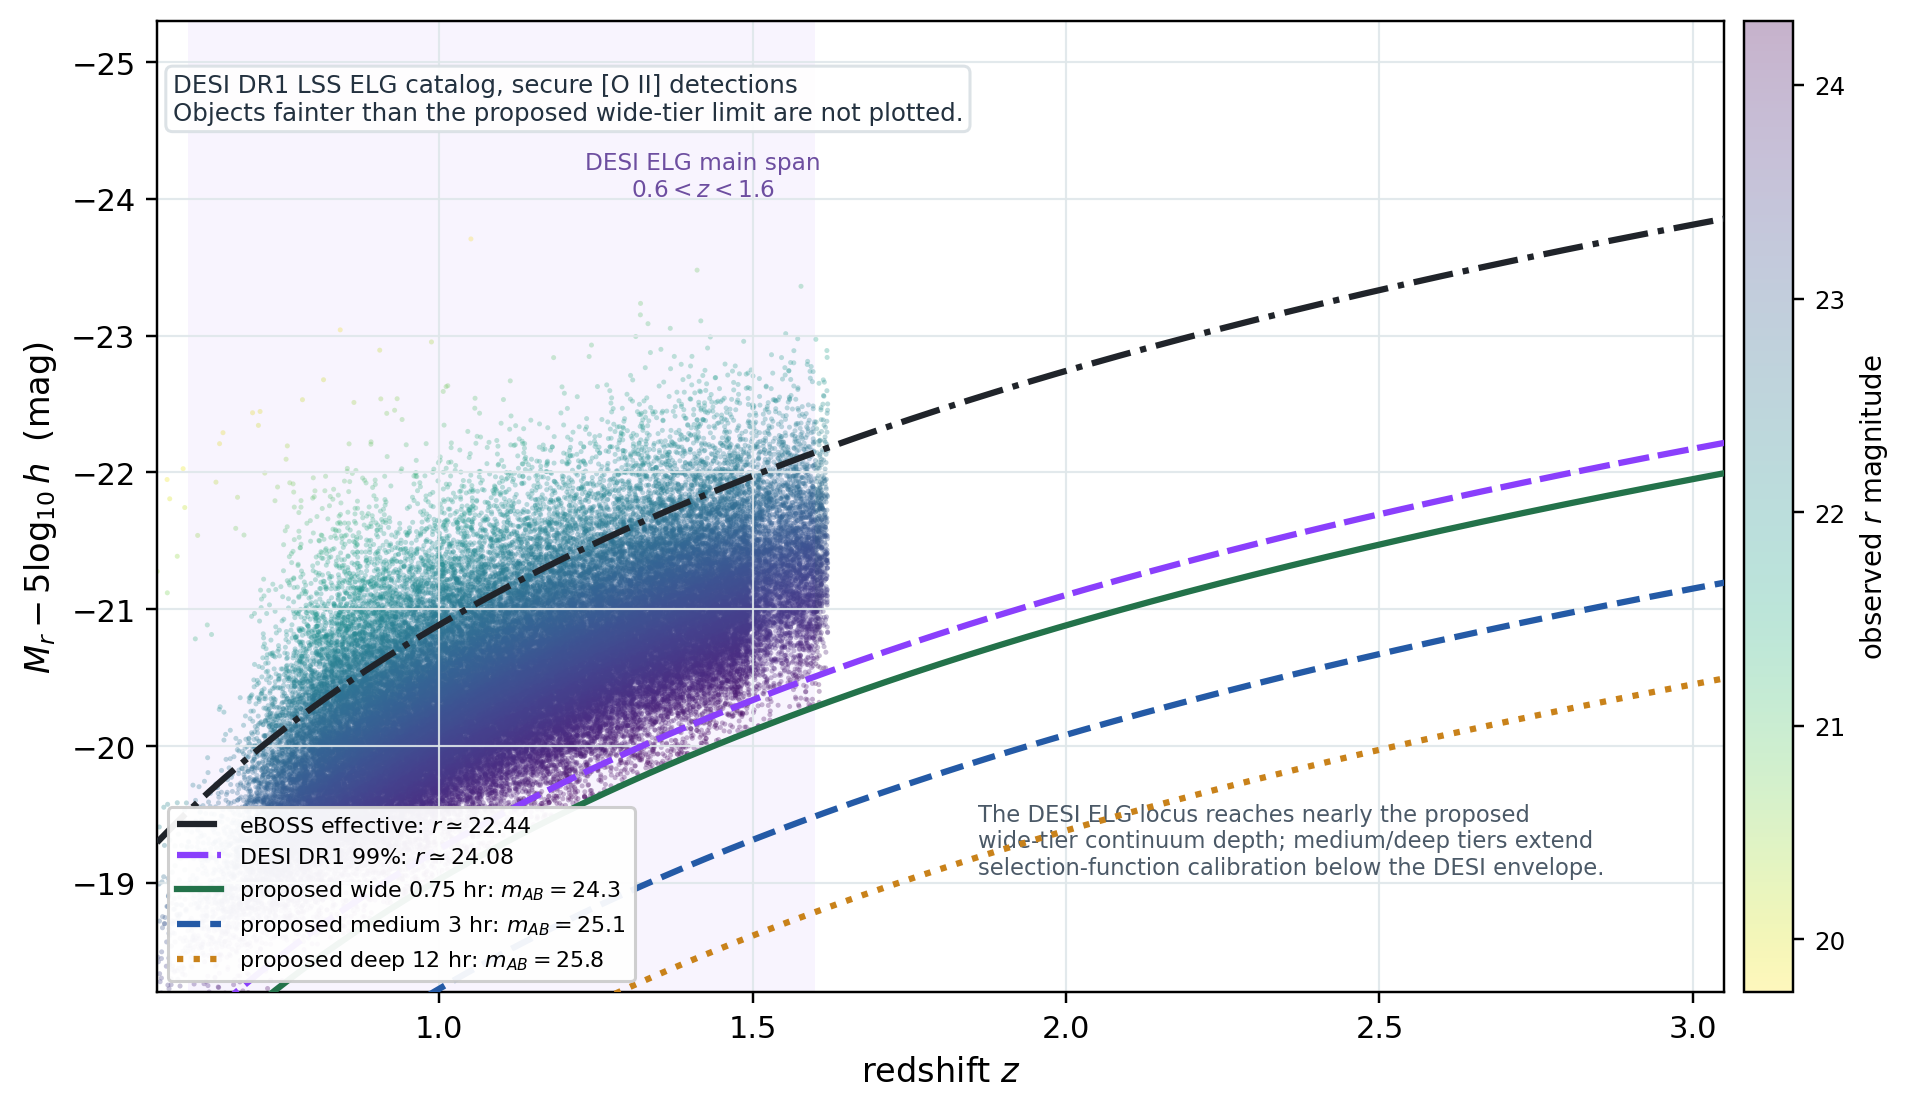
\includegraphics[width=0.78\textwidth]{elg_absmag_depth_catalog.png}
\caption{Observed-frame ELG absolute magnitude from the DESI DR1 LSS ELG catalog, shown against redshift. Points are secure DESI ELGs with [O\,II] detections and $m_r\le24.3$. Fainter objects are not plotted. The black curve shows the effective eBOSS depth for comparison, while the purple curve shows the DESI DR1 99th-percentile $r$-band depth of the plotted sample. The green, blue, and orange curves show the faintest $M_r-5\log_{10}h$ reachable at the proposed wide, medium, and deep continuum limits. This is a planning comparison in observed $r$ band and omits $K$-corrections \cite{raichoor2022}.}
\label{fig:elgmagdepth}
\end{figure}

To convert Figure~\ref{fig:elgmagdepth} into a redshift-dependent count estimate, we bin the same secure DESI sample in $M_r-5\log_{10}h$ and redshift. The observed-frame continuum luminosity function is
\begin{equation}
  \widehat{\Phi}_M(M_k,z_j)=
  \frac{N_k}
  {\Omega_{\rm eff}\,V_{\rm c,deg^2}(z_1,z_2)\,\Delta M},
\end{equation}
with the same $\Omega_{\rm eff}$ and cosmology used for the [O\,II] LF anchor above. Figure~\ref{fig:desiMlf} shows the resulting evolution over $0.6<z<1.6$. The turnover at faint $M_r$ is not the galaxy LF turnover. It is the DESI target-selection and redshift-success boundary. This is why the figure is useful for planning depth, but not sufficient by itself for extrapolating medium/deep-tier yields.

\begin{figure}[tp]
\centering
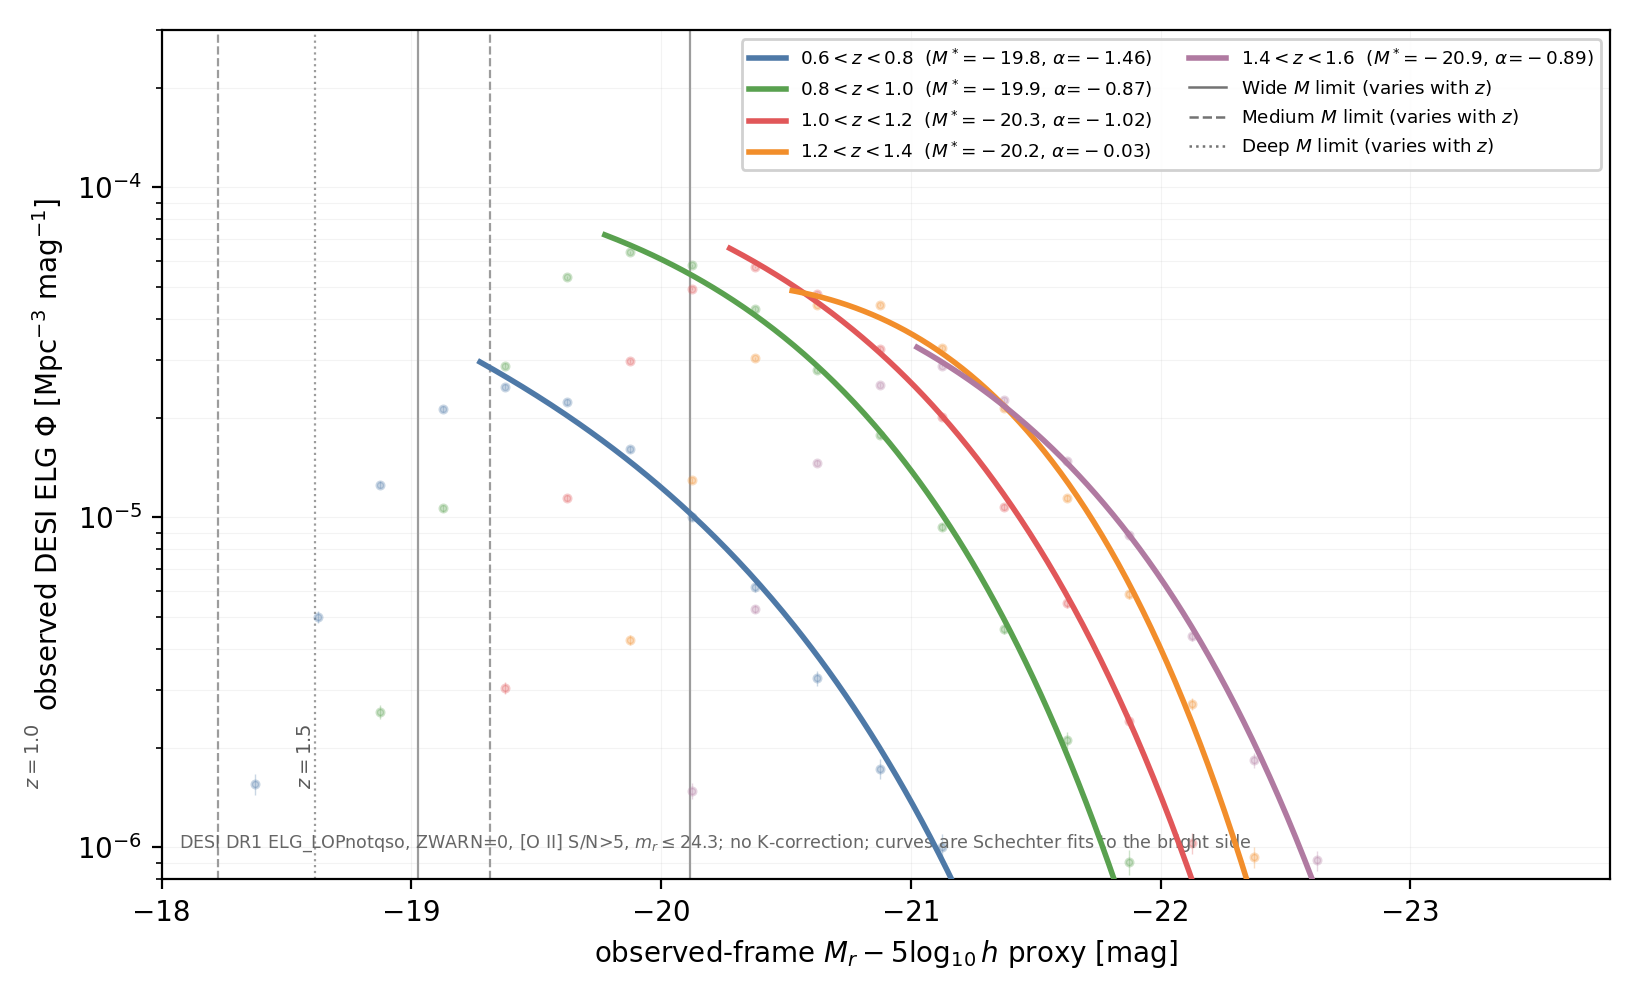
\includegraphics[width=0.78\textwidth]{desi_elg_lf_proxy_evolution.png}
\caption{Observed-frame DESI ELG absolute-magnitude luminosity function in redshift bins from the same secure \texttt{ELG\_LOPnotqso} sample as Figure~\ref{fig:elgmagdepth}. Faint points are the binned luminosity function, solid curves Schechter fits ($\Phi^\star,M^\star,\alpha$) to the well-sampled bright side of each bin, restricted to magnitudes brighter than the faint-end turnover set by DESI target selection rather than the galaxy population. The curves should not be extrapolated through that incompleteness edge. Vertical markers show the proposed continuum limits at representative redshifts. These remain DESI-observed, not $K$-corrected rest-frame, luminosity functions \cite{raichoor2022}.}
\label{fig:desiMlf}
\end{figure}

The corresponding DESI-observed count integral is listed in Table~\ref{tab:desiMcounts}. It answers a narrower question than the line-flux table. For a source already represented in the DESI ELG selection, how many objects per \fovlarge\ frame lie above the proposed continuum depth? The nearly identical wide, medium, and deep counts are a diagnostic, not a claim that depth is unimportant. They show that the DESI parent catalog itself is already truncated near the wide-tier depth. Hence, DESI alone cannot measure the incremental population expected at $m_{\rm AB}\simeq25.1$--26.6.

\begin{table}[tp]
\centering
\sffamily\scriptsize
\begin{tabularx}{\textwidth}{@{}c c c c c c c@{}}
\toprule
\textbf{$z$ bin} &
\textbf{$M_{\rm lim,wide}$} & \textbf{$N_{\rm frame,wide}$} &
\textbf{$M_{\rm lim,med}$} & \textbf{$N_{\rm frame,med}$} &
\textbf{$M_{\rm lim,deep}$} & \textbf{$N_{\rm frame,deep}$}\\
 & \multicolumn{1}{c}{$m_r=24.3$} & \multicolumn{1}{c}{0.25 deg$^2$} &
   \multicolumn{1}{c}{$m_r=25.1$} & \multicolumn{1}{c}{0.25 deg$^2$} &
   \multicolumn{1}{c}{$m_r=25.8$} & \multicolumn{1}{c}{0.25 deg$^2$}\\
\midrule
0.6--0.8 & -18.07 & 8.9 & -17.27 & 8.9 & -16.57 & 8.9\\
0.8--1.0 & -18.74 & 29.6 & -17.94 & 29.7 & -17.24 & 29.7\\
1.0--1.2 & -19.28 & 29.6 & -18.48 & 29.7 & -17.78 & 29.7\\
1.2--1.4 & -19.73 & 26.0 & -18.93 & 26.1 & -18.23 & 26.1\\
1.4--1.6 & -20.11 & 17.2 & -19.31 & 17.3 & -18.61 & 17.3\\
\bottomrule
\end{tabularx}
\caption{DESI-observed continuum count integral corresponding to Figures~\ref{fig:elgmagdepth} and \ref{fig:desiMlf}. The count is $N_{\rm frame}=0.25\,\Sigma$ after integrating the binned DESI observed-frame luminosity function brighter than the listed $M_r-5\log_{10}h$ limit. Because the local DESI catalog used here was clipped at $m_r\le24.3$, the medium and deep columns are lower limits and mainly flag where external deep surveys must supply the missing faint population.}
\label{tab:desiMcounts}
\end{table}

The required external calibration is therefore not optional. DESI gives the wide-area normalization and the $0.6<z<1.6$ color-selected ELG anchor, while DEEP2, VVDS, and COSMOS-based emission-line catalogs supply the fainter continuum and higher-redshift information needed to model the DESI truncation boundary, color incompleteness, and faint-end LF slope, with the zCOSMOS group catalog adding environment and membership context \cite{newman2013deep2,lefevre2013vvds,saito2020,knobel2012zcosmos}. Literature [O\,II], H$\beta$+[O\,III], and H$\alpha$ LF measurements show strong redshift evolution in both $L^\star$ and normalization. Therefore, the final yield model should be a joint fit to DESI plus these deeper samples rather than a pure extrapolation of the DESI observed-frame luminosity function \cite{comparat2015,comparat2016,khostovan2015,mehta2015}.

\subsection{Wedding-Cake Survey Strategy}

The BAO/RSD program is organized as a wedding-cake survey. It has a very wide tier for cosmological volume, a medium tier for redshift-success calibration and fainter ELGs, and a deep pencil-beam tier for luminosity-function tails, completeness calibration, and deblending stress tests.

\begin{figure}[tp]
\centering
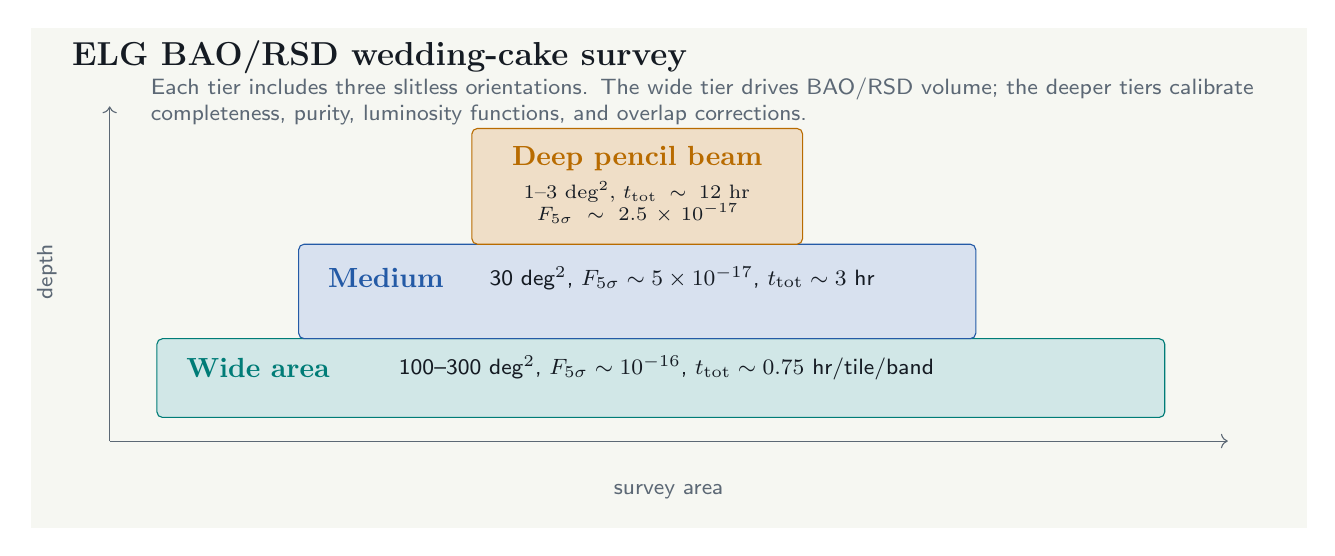
\begin{tikzpicture}[font=\sffamily\footnotesize]
  \fill[paper] (-0.4,-0.35) rectangle (15.8,6.0);
  \node[anchor=west,font=\bfseries\large,color=ink] at (0,5.62) {ELG BAO/RSD wedding-cake survey};
  \draw[->,color=muted] (0.6,0.75) -- (14.8,0.75);
  \draw[->,color=muted] (0.6,0.75) -- (0.6,5.0);
  \node[anchor=north,color=muted] at (7.7,0.32) {survey area};
  \node[rotate=90,anchor=south,color=muted] at (0.05,2.9) {depth};

  \fill[teal!18,draw=teal,rounded corners=2pt] (1.2,1.05) rectangle (14.0,2.05);
  \fill[blue!18,draw=blue,rounded corners=2pt] (3.0,2.05) rectangle (11.6,3.25);
  \fill[gold!22,draw=gold,rounded corners=2pt] (5.2,3.25) rectangle (9.4,4.72);

  \node[anchor=west,font=\bfseries,color=teal] at (1.45,1.68) {Wide area};
  \node[anchor=west,color=ink] at (4.15,1.68) {100--300 deg$^2$, $F_{5\sigma}\sim10^{-16}$, $t_{\rm tot}\sim0.75$ hr/tile/band};
  \node[anchor=west,font=\bfseries,color=blue] at (3.25,2.82) {Medium};
  \node[anchor=west,color=ink] at (5.3,2.82) {30 deg$^2$, $F_{5\sigma}\sim5\times10^{-17}$, $t_{\rm tot}\sim3$ hr};
  \node[font=\bfseries,color=gold] at (7.3,4.34) {Deep pencil beam};
  \node[align=center,color=ink,font=\scriptsize,text width=3.9cm] at (7.3,3.78)
    {1--3 deg$^2$, $t_{\rm tot}\sim12$ hr\\ $F_{5\sigma}\sim2.5\times10^{-17}$};

  \node[anchor=west,text width=14.0cm,color=muted] at (1.0,5.06)
  {Each tier includes three slitless orientations. The wide tier drives BAO/RSD volume; the deeper tiers calibrate completeness, purity, luminosity functions, and overlap corrections.};
\end{tikzpicture}
\caption{The ELG program is not a single-depth survey. It is a layered BAO/RSD experiment in which deeper pencil beams calibrate the wide-area selection function. The quoted line-flux depths $F_{5\sigma}$ are in erg s$^{-1}$ cm$^{-2}$.}
\label{fig:weddingcake}
\end{figure}

Table~\ref{tab:wedding} turns the wedding-cake strategy in Figure~\ref{fig:weddingcake} into exposure and depth requirements. The wide tier supplies the BAO/RSD volume, while the medium, deep, and ultra-deep tiers are included to measure redshift failures, overlap losses, and luminosity-function tails that cannot be calibrated from the wide survey alone.

\begin{table}[tp]
\centering
\sffamily\small
\begin{tabularx}{\textwidth}{@{}p{2.5cm}p{2.4cm}p{2.8cm}p{3.1cm}Y@{}}
\toprule
\textbf{Tier} & \textbf{Area} & \textbf{3-orientation exposure} & \textbf{Line-flux limit $F_{5\sigma}$} & \textbf{Primary role}\\
 & deg$^2$ & science time per band & erg s$^{-1}$ cm$^{-2}$ (smaller $=$ deeper) & \\
\midrule
Wide BAO/RSD & 100 \degti threshold; 300 \degti goal & $3\times900$ s per band & $1.0\times10^{-16}$ & Cosmological volume; $10^6$--$3\times10^6$ secure ELG redshifts.\\
Medium calibration & 30 \degti & $3\times3600$ s per band & $5.0\times10^{-17}$ & Redshift failures, faint ELGs, line-ratio priors, survey transfer functions.\\
Deep pencil beam & 1--3 \degti & $3\times4$ hr per band & $2.5\times10^{-17}$ & Luminosity-function tail, overlap calibration, completeness to $z\simeq3$.\\
Ultra-deep validation & 0.1--0.3 \degti & $3\times16$ hr per band & $1.3\times10^{-17}$ & External spectroscopic reference fields and pipeline robustness tests.\\
\bottomrule
\end{tabularx}
\caption{Illustrative ELG survey tiers. Exposure times are total science exposure per filter/band and include the required three orientations, but not slew, readout, dither, calibration, or scheduling overhead. The line-flux limit $F_{5\sigma}$ is a faint-detection threshold. Hence, a \emph{smaller} value means a fainter line is still detected, i.e. greater depth. Because the survey is background-limited, $F_{5\sigma}\propto t_{\rm tot}^{-1/2}$. Therefore, the longer-exposure tiers reach fainter limits and are deeper, not shallower: the wide tier at $3\times900$ s reaches $1.0\times10^{-16}$, whereas the ultra-deep tier at $3\times16$ hr reaches $1.3\times10^{-17}$, nearly an order of magnitude fainter.}
\label{tab:wedding}
\end{table}

\subsection{BAO, \texorpdfstring{$H_0$}{H0}, and Growth Precision}

The ELG BAO measurement is designed as a precision distance-ratio experiment. In each redshift bin the measured parameters are
\begin{equation}
  \alpha_\perp(z)=
  \frac{[D_M(z)/r_d]}{[D_M(z)/r_d]_{\rm fid}},\qquad
  \alpha_\parallel(z)=
  \frac{[H(z)r_d]_{\rm fid}}{H(z)r_d},
\end{equation}
where $D_M$ is the transverse comoving distance and $r_d$ is the sound horizon at the drag epoch. Therefore the survey does not measure an absolute $H_0$ by itself unless a sound-horizon calibration is supplied by CMB, BBN, or another early-universe prior. Without that prior, the clean late-time observable is the inverse-distance-ladder combination $H_0r_d$.

The growth measurement comes from the redshift-space galaxy power spectrum,
\begin{equation}
  P_s(k,\mu,z)\simeq
  \left[b(z)+f(z)\mu^2\right]^2 P_m(k,z)
  \exp\!\left[-k^2\mu^2\sigma_r^2(z)\right],
\end{equation}
with $\sigma_r=c\,\sigma_z/H(z)$ the radial redshift-smearing scale. The principal growth observable is $\fsig(z)$. For compact reporting we also quote a growth-amplitude summary,
\begin{equation}
  S_8^{\rm grow}\equiv \sigma_8(\Omega_m/0.3)^{1/2},
\end{equation}
after marginalizing over galaxy bias in the ELG clustering model. The statistical power scales approximately as
\begin{equation}
  V_{\rm eff}(k,\mu)=
  \int \left[\frac{n(z)P(k,\mu,z)}{1+n(z)P(k,\mu,z)}\right]^2 dV,
\end{equation}
so the wide tier sets the cosmological precision while the medium and deep tiers reduce redshift-failure and line-identification systematics.

In configuration space the same information is measured from the two-dimensional galaxy correlation function, using the minimum-variance Landy--Szalay estimator \cite{landyszalay1993},
\begin{equation}
  \xi(\sigma,\pi)=\frac{DD(\sigma,\pi)-2DR(\sigma,\pi)+RR(\sigma,\pi)}
  {RR(\sigma,\pi)},
  \label{eq:xiestimator}
\end{equation}
where $\sigma$ is the transverse separation and $\pi$ is the line-of-sight separation. The BAO feature appears as an annular excess at $r_{\rm BAO}\simeq100$--$110\,h^{-1}$ Mpc. In real space this ring is nearly circular. In redshift space, peculiar velocities and coherent infall distort the contours, producing the anisotropy which is modeled jointly with the BAO scale. The transverse and radial BAO positions give
\begin{equation}
  \sigma_{\rm BAO}\propto D_M(z)/r_d,\qquad
  \pi_{\rm BAO}\propto [H(z)r_d]^{-1},
\end{equation}
while the quadrupole-to-monopole structure of $\xi(\sigma,\pi)$ constrains $\fsig(z)$. The ELG survey is therefore designed to recover the full two-dimensional correlation function, not only a spherically averaged BAO peak.

\begin{figure}[tp]
\centering

\includegraphics[width=0.80\textwidth]{gal_corr_hr4.png}
\caption{Two-dimensional galaxy correlation function $\xi(\sigma,\pi)$ in redshift space, both panels drawn to a common $\pm130\,h^{-1}$\,Mpc radius on the same $\log_{10}|\xi|$ color scale. Left: the observed BOSS CMASS-North catalog, 568{,}776 galaxies against 5{,}000{,}000 randoms with the Landy--Szalay estimator of Eq.~\eqref{eq:xiestimator}, with the solid circle marking its fitted BAO ridge at $s\simeq105\,h^{-1}$\,Mpc. Right: the Horizon Run 4 mock galaxy catalog \cite{hr4}, rendered directly from the author's pair-count measurement, with the solid circle marking its BAO ridge at $s\simeq107\,h^{-1}$\,Mpc. The mock reproduces the same redshift-space distortion signature seen in the real data, the small-scale fingers of god along $\pi$ and the large-scale Kaiser squashing. Therefore, the clustering pipeline used for the ELG forecast is shown recovering the expected anisotropy directly from real galaxies first.}
\label{fig:hr4xi}
\end{figure}

Operationally, the clustering analysis will fit $\xi(\sigma,\pi)$ in redshift slices using mock-derived covariance matrices and survey random catalogs. The fitted parameters are the two dilation factors $(\alpha_\perp,\alpha_\parallel)$, nuisance broadband terms, galaxy bias, redshift smearing, and RSD parameters. The recovered $(D_M/r_d,Hr_d,\fsig)$ values are then propagated into cosmological models such as flat $\Lambda$CDM, $w_0w_a$ dark energy, and modified-growth parameterizations. This is the direct path from the observed ELG redshift catalog to constraints on $H_0$, the expansion history, and the growth factor.

The percentage precisions in Table~\ref{tab:baoforecast} are planning scalings, not the output of a full Fisher matrix. The threshold case is normalized to a conservative BAO/RSD performance target for a 100 deg$^2$, $N_{\rm ELG}\sim10^6$ high-purity redshift survey. The target is 1.5--2.5\% per broad redshift bin in the BAO dilation parameters and 4--6\% per bin in $\fsig$. The goal case is then scaled with effective survey volume,
\begin{equation}
  \sigma_{\rm stat,goal}\simeq
  \sigma_{\rm stat,thr}
  \left(\frac{V_{\rm eff,thr}}{V_{\rm eff,goal}}\right)^{1/2},
\end{equation}
where $V_{\rm eff}$ is the quantity defined above. If the usable area and secure-redshift count both increase from 100 deg$^2$ and $\sim10^6$ to 300 deg$^2$ and $\sim3\times10^6$, the ideal statistical improvement is close to $3^{1/2}$. Hence, a 1.5--2.5\% threshold BAO-bin precision becomes about 0.9--1.5\% and a 4--6\% threshold $\fsig$ precision becomes about 2.5--4\%. The combined-distance entries are slightly tighter because they represent the multi-bin distance-scale constraint after combining transverse and radial BAO information while retaining a floor for redshift failures, line confusion, and survey-window calibration. The quoted $H_0$ values are not direct late-time measurements of $H_0$ alone. They are obtained by adding the combined BAO distance precision and an assumed external sound-horizon calibration in quadrature,
\begin{equation}
  \left(\frac{\sigma_{H_0}}{H_0}\right)^2
  \simeq
  \left(\frac{\sigma_{\rm BAO}}{\alpha}\right)^2+
  \left(\frac{\sigma_{r_d}}{r_d}\right)^2 ,
\end{equation}
with $\sigma_{r_d}/r_d$ taken to be of order 1--2\% for the proposal-level estimate. The final row keeps the same wide-area statistical BAO scale but lowers the systematic allowance after applying the medium/deep calibration tiers. This is why it improves the $H_0$ and growth floors without claiming a larger wide-survey volume.

\begin{table}[tp]
\centering
\sffamily\small
\begin{tabularx}{\textwidth}{@{}p{3.0cm}p{2.2cm}p{2.4cm}p{2.8cm}Y@{}}
\toprule
\textbf{Survey configuration} & \textbf{Secure ELGs and required survey period} & \textbf{BAO distance precision} & \textbf{$H_0$ precision} & \textbf{Growth precision}\\
area in deg$^2$; redshift dimensionless & counts; calendar yr; exposure hr & fractional \% & fractional \% & fractional \%\\
\midrule
Threshold wide survey: 100 \degti, $1<z<3$ & $\sim10^6$; 1.5--2.5 yr calendar time, about 1200--1800 hr science exposure including three orientations & $1.5$--$2.5\%$ per broad bin in $D_M/r_d$ and $H r_d$; $1.5$--$2.0\%$ combined distance scale & $2.5$--$3.5\%$ with external $r_d$ prior; otherwise $H_0r_d$ only & $\sigma(\fsig)=4$--$6\%$ per bin; $S_8^{\rm grow}$ to $\sim4\%$ after bias marginalization\\
Goal wide survey: 300 \degti, $1<z<3$ & $\sim3\times10^6$; 3--4 yr calendar time, about 2000--3000 hr science exposure including three orientations & $0.9$--$1.5\%$ per broad bin; $0.9$--$1.2\%$ combined distance scale & $1.5$--$2.2\%$ with external $r_d$ prior; $H_0r_d$ at roughly the same fractional precision & $\sigma(\fsig)=2.5$--$4\%$ per bin; $S_8^{\rm grow}$ to $\sim2.5$--$3.5\%$\\
Goal plus calibrated wedding-cake tiers & $\sim3\times10^6$ wide plus fainter calibration samples; 4--5 yr total ELG program, about 3000--4200 hr science exposure & Same statistical BAO scale as goal wide survey, but with reduced redshift-failure and purity bias & $1.3$--$2.0\%$ if the selection-function systematics remain subdominant and $r_d$ is externally calibrated & $2$--$3\%$ growth-amplitude floor targeted by overlap calibration, mock recovery, and bias modeling\\
\bottomrule
\end{tabularx}
\caption{Planning-level cosmological precision and required survey period from the ELG BAO/RSD program. These are proposal forecasts, not final Fisher-matrix requirements. They assume high-purity redshifts, three-orientation overlap correction, realistic survey masks, and external calibration of $r_d$ when quoting absolute $H_0$.}
\label{tab:baoforecast}
\end{table}

The science requirement is therefore not simply to detect many emission lines. It is to recover the BAO scale and the anisotropic RSD signal without imprinting a roll-angle, morphology, or overlap-dependent selection function. The baseline requirement is redshift purity $>98\%$ for the cosmology sample, catastrophic line-confusion rate $<1\%$, and a redshift-success model whose spatial variation is known well enough that the induced BAO-scale distance bias remains below $0.3\%$. These requirements will be verified by blinded image-level simulations and by repeated reductions of the same fields using only two of the three orientations with the third orientation held out as a validation data set.

\subsection{Parameter-Estimation Pipeline: Redshifts to Cosmological Constraints}

The redshift catalog and the clustering statistics defined above are not yet a cosmological measurement. Four further stages connect them to a posterior on $H_0r_d$, $\Omega_m$, $w_0$, $w_a$, and $S_8^{\rm grow}$. First, each deblended spectrum is converted into a redshift and a quality flag. Second, the redshift catalog is compressed into two-point clustering statistics in configuration and Fourier space. Third, a covariance matrix is built for those statistics. Fourth, a likelihood is constructed and sampled. This subsection defines each stage explicitly, extending the forecast of Table~\ref{tab:baoforecast} into an analysis plan. The End-to-End Validation exercise below runs this same plan on image-level mocks before it is applied to real survey data. Not every tool named below is load-bearing for that forecast. The Gaussian likelihood sampled with an affine-invariant ensemble MCMC is what the Table~\ref{tab:baoforecast} numbers themselves rest on. CosmoMC and Cobaya extend the same likelihood to the joint multi-probe fit. Nested sampling is invoked only where a Bayesian evidence comparison is specifically required. The neural power-spectrum emulator exists because that nested-sampling run is otherwise too expensive to evaluate directly. The simulation-based inference channel is an independent cross-check the planning precision does not depend on. Each is introduced below at the point where its own necessity, not general best practice, requires it.

\subsubsection{Redshift and Quality Classification}

Each deblended one-dimensional spectrum from the scene-reconstruction pipeline (Section~\ref{sec:effres}) is redshifted by $\chi^2$ template fitting against a library of ELG templates spanning the H$\alpha$/[O\,III]/[O\,II] flux-ratio sequence, following the same template classification-and-redshift approach as the BOSS/eBOSS spectroscopic pipeline \cite{bolton2012}. A supervised deep-learning classifier runs in parallel, trained on labeled DESI and SDSS spectra together with the injected slitless simulations of the End-to-End validation suite below, in the spirit of QuasarNET, the convolutional network which locates line positions, classifying quasar spectra \cite{quasarnet2018}. The template fit supplies the redshift and its formal uncertainty. The classifier flags the catastrophic degeneracy that a $\chi^2$ grid search cannot resolve on its own, a single bright line mistaken for a different transition at a different redshift. It draws on the joint multi-line pattern, the morphology prior, and the redundancy across the three observed position angles already captured by the scene model of Eq.~\eqref{eq:scene}. The two outputs are combined into the redshift quality flag already defined in the science catalog (Section~\ref{sec:effres}), which sets the $>98\%$-purity cosmology sample required above.

\subsubsection{Two-Point Clustering Estimators in Configuration and Fourier Space}

The correlation function of Eq.~\eqref{eq:xiestimator} is measured with random catalogs that encode the survey mask, the overlap losses between the three position angles, and the redshift-dependent selection function. The same information is measured independently in Fourier space. The FKP-weighted density field
\begin{equation}
  F(\mathbf{r}) = w(\mathbf{r})\big[n_g(\mathbf{r})-\alpha_{\rm rand}\,n_s(\mathbf{r})\big],
  \qquad
  w(\mathbf{r}) = \frac{1}{1+n(\mathbf{r})P_0},
  \label{eq:fkp}
\end{equation}
sets $n_g$ and $n_s$ as the galaxy and synthetic random densities and $\alpha_{\rm rand}$ as their relative normalization \cite{fkp1994}. It yields minimum-variance power-spectrum multipoles $P_0(k)$, $P_2(k)$, and $P_4(k)$ through the Yamamoto line-of-sight estimator implemented with fast Fourier transforms \cite{yamamoto2006,hand2017nbodykit}. The power-spectrum multipoles and the correlation-function wedges are fit for the same $(\alpha_\perp,\alpha_\parallel,\fsig)$ parameters. Therefore, agreement between the configuration-space and Fourier-space results is a direct internal test for residual systematics, including window-function mismodeling, redshift-failure gradients, and position-angle-dependent selection effects.

\subsubsection{Covariance Matrices}\label{sec:covariance}

The likelihood requires a covariance matrix for the compressed BAO/RSD parameters in each redshift bin. The baseline covariance is built from an ensemble of mock galaxy catalogs constructed on N-body simulations at the resolution and volume of Horizon Run 4 \cite{hr4}, populated with an ELG halo-occupation model tuned to the luminosity functions of Section~\ref{sec:elgdepth}, and passed through the same selection function, masks, and redshift-quality cuts as the real survey. A faster ensemble of approximate mocks, calibrated against the smaller set of full N-body realizations, supplies the larger number of realizations needed to invert a well-conditioned covariance matrix. Internal jackknife resampling of the survey footprint provides an independent, mock-free covariance estimate used to validate the mock-based one before it enters the likelihood.

\subsubsection{Likelihood, MCMC, and Simulation-Based Inference}

The baseline likelihood is Gaussian in the compressed parameters,
\begin{equation}
  -2\ln\mathcal{L} =
  \big[\mathbf{p}_{\rm obs}-\mathbf{p}_{\rm model}(\theta)\big]^{T}
  \mathbf{C}^{-1}
  \big[\mathbf{p}_{\rm obs}-\mathbf{p}_{\rm model}(\theta)\big],
  \label{eq:gausslike}
\end{equation}
with $\mathbf{p}=(\alpha_\perp,\alpha_\parallel,\fsig)$ per redshift bin, $\mathbf{C}$ the covariance of Section~\ref{sec:covariance}, and $\theta$ the cosmological and nuisance parameters. For the ELG-only fit the posterior is sampled with an affine-invariant ensemble MCMC sampler \cite{emcee2013}. For the joint fit that adds Planck/ACT CMB priors and the internal SN\,Ia and DSPL strong-lensing likelihoods of the companion programs above, the same posterior is sampled with the CosmoMC and Cobaya cosmological-parameter-estimation codes \cite{lewisbridle2002,torradolewis2021},
\begin{equation}
  \mathcal{P}(\theta\mid D) \;\propto\;
  \mathcal{L}_{\rm ELG}(D_{\rm ELG}\mid\theta)\,
  \mathcal{L}_{\rm SN}(D_{\rm SN}\mid\theta)\,
  \mathcal{L}_{\rm lens}(D_{\rm lens}\mid\theta)\,
  \mathcal{L}_{\rm CMB}(D_{\rm CMB}\mid\theta)\,
  \Pi(\theta),
  \label{eq:jointpost}
\end{equation}
with $\Pi(\theta)$ the prior on $\theta$, recovering the joint constraint on $H_0$, $\Omega_m$, and $(w_0,w_a)$ already anticipated in the supernova program above. Where a Bayesian model comparison between flat $\Lambda$CDM and dynamic dark energy is required, the same likelihood is instead sampled with nested sampling \cite{polychord2015}, which returns the evidence directly rather than only the posterior. A joint, multi-probe nested-sampling run can require $10^6$--$10^7$ likelihood evaluations. Therefore, the nonlinear matter power spectrum entering Eq.~\eqref{eq:gausslike} is evaluated with a neural emulator trained on outputs from Boltzmann and perturbation-theory codes \cite{cosmopower2022,euclidemulator2021} rather than recomputed from scratch at every step, reducing each theory evaluation from a full nonlinear-power-spectrum calculation to a millisecond-scale forward pass.

A second, likelihood-free channel cross-checks the Gaussian result. The same simulation-based inference machinery proposed for the strong-lensing hierarchical layer above trains a neural density estimator directly on the full mock $P(k,\mu)$ or $\xi(\sigma,\pi)$ realizations from the covariance ensemble \cite{cranmer2020}, learning the mapping from cosmological parameters to the clustering statistics without assuming a Gaussian likelihood or a hand-derived covariance. This channel is not required to reach the planning precision of Table~\ref{tab:baoforecast}. That forecast is scoped on the standard Gaussian pipeline above. The simulation-based channel instead lets the analysis use non-Gaussian small-scale information, for example the mildly nonlinear fingers-of-god signal, as an independent growth-rate cross-check rather than a term the Gaussian covariance must marginalize away.

Before unblinding, a fixed but undisclosed offset is applied to $(\alpha_\perp,\alpha_\parallel,\fsig)$ in the catalog, following the blind-analysis practice of BOSS, eBOSS, and DESI. The offset is removed only after the pipeline, the covariance, and the likelihood have been frozen, extending the held-out-orientation validation of the observing strategy above into the cosmological analysis itself.

\subsection{End-to-End Validation}\label{sec:e2eval}

The survey must be proven by simulated images, not by analytic exposure-time arguments alone. None of the purity, completeness, or flux-bias numbers quoted above as requirements has yet been demonstrated at survey scale. Figure~\ref{fig:crowded} illustrates the baseline deblending geometry and method on a single tile. Figure~\ref{fig:slicer} illustrates an image-slicer alternative. Neither yet provides the recovery statistics that would validate it. The joint sparse inversion's computational cost at the scale of the full survey (roughly $10^6$--$3\times10^6$ objects across $10^4$ roll-visits) has not yet been characterized. The Phase A validation suite should inject realistic galaxies into detector scenes, recovering redshifts with the same pipeline planned for flight. The required outputs, which this proposal treats as requirements to be verified rather than results in hand, are:
\begin{itemize}
  \item redshift completeness, purity, and catastrophic-failure rates;
  \item single-line misidentification rates for H$\alpha$, [O\,III], and [O\,II];
  \item morphology-induced wavelength shifts and line broadening;
  \item overlap statistics for \fovsmall\ and \fovlarge\ fields;
  \item the effect of roll angle, dithering, and direct-image priors;
  \item random catalogs, masks, and survey-window functions for clustering;
  \item blinded recovery of BAO scale and $\fsig(z)$ from image-level mocks;
  \item wall-clock and memory cost of the joint scene-reconstruction inversion (Eq.~\eqref{eq:scene}) per tile and extrapolated to the full survey, to establish whether the baseline pipeline is computationally tractable for the full survey.
\end{itemize}

\subsection{Synergy with Legacy Deep Fields}\label{sec:deepfields}

The two high-Galactic-latitude caps which anchor the wide survey were chosen not only to avoid the Milky Way but to enclose the richest legacy deep fields in the sky (Figure~\ref{fig:skymap}). The north cap contains COSMOS, GOODS-N, the Extended Groth Strip, and the Subaru Deep Field. The south cap contains GOODS-S with the Hubble Ultra Deep Field together with the UDS/SXDS and XMM-LSS fields. These fields hold decades of deep HST and Subaru imaging, extensive ground and space spectroscopy, and now JWST coverage from CEERS in the Extended Groth Strip, JADES in GOODS-S, and COSMOS-Web. Therefore, the wide survey inherits an unusually complete set of ancillary data over its own footprint. Within each cap the $100$--$300$ deg$^2$ wide tier and its nested medium and deep tiers are located on a high-Galactic-latitude legacy concentration, the NDWFS/HETDEX Bo\"otes field ($b\simeq+67^\circ$) in the north and the SXDS/UDS/XMM-LSS deep field ($b\simeq-59^\circ$) in the south (Figure~\ref{fig:deepzoom}). Both were chosen at high $|b|$ to stay clear of Galactic extinction and cirrus. The Bo\"otes anchor is particularly valuable because the HETDEX blind emission-line survey covers the same field, giving a direct external comparison sample for the slitless emission-line selection while the remaining legacy fields lie elsewhere in the same caps and anchor additional deep and calibration pointings.

\begin{figure}[tp]
\centering

\includegraphics[width=0.92\textwidth]{elg_skymap.png}
\caption{Proposed ELG survey fields on an equatorial Mollweide projection, background the real Planck 857\,GHz thermal-dust map \cite{planck2018hfi} (native $\sim$5$'$ resolution, CDS \textit{hips2fits}) with its intensity scale below. The north and south Galactic caps ($|b|\gtrsim45^\circ$, green and blue outlines) avoid the Milky Way zone ($|b|<20^\circ$, red curves) and lie within the DESI, Euclid, Rubin/LSST, and Roman footprints. Orange open boxes mark the two ELG wide-tier footprints at true scale ($\sim$150\,deg$^2$ each), both in dark low-cirrus windows. Cyan squares mark the two ultra-deep imaging fields, the Planck-minima anchors of Figure~\ref{fig:imgfields}, shown as symbols since at $2.25$\,deg$^2$ they are far smaller than the ELG tiers. Red diamonds mark the two SN Ia time-domain cadence fields ($\sim$5--10\,deg$^2$ each), nested inside each wide tier so SN hosts inherit real slitless redshifts from the flagship survey (zoomed in Figure~\ref{fig:deepzoom}). Magenta outlines mark the imaging-only wide-extension fields ($\sim$306\,deg$^2$ per cap), beside the Lockman Hole in the north and the south Galactic pole in the south. Gold stars mark legacy HST and Subaru deep fields within the caps (Figure~\ref{fig:deepzoom}).}
\label{fig:skymap}
\end{figure}

\begin{figure}[tp]
\centering

\includegraphics[width=0.98\textwidth]{elg_deepfields_zoom.png}
\caption{Nested wedding-cake tiers of the proposed ELG survey, one Galactic cap per panel, in gnomonic (TAN) projection on the Planck 857\,GHz thermal-dust map \cite{planck2018hfi} (native $\sim$5$'$ resolution, CDS \textit{hips2fits}). Both anchors, the NDWFS/HETDEX Bo\"otes field ($b\simeq+67^\circ$) and the SXDS/UDS/XMM-LSS field ($b\simeq-59^\circ$), sit in dark low-cirrus windows. The bright complex at the upper left of the southern panel, toward Taurus, illustrates the foreground the field selection avoids. Neighbouring legacy fields (ELAIS-N1, the Extended Groth Strip, the Subaru Deep Field, GOODS-S) are shown for context. Each $\pm4^\circ$ inset zooms on the anchor and shows the true footprint shape of the legacy fields together with the wedding-cake nesting. The wide tier ($\sim$150 deg$^2$, gold) encloses the medium tier (30 deg$^2$, orange), which encloses the deep tier (1--3 deg$^2$, red). Each tier is a square paving of $30'\times30'$ tiles rather than a circle. The red outline inside each wide tier is the SN Ia time-domain cadence field ($\sim$7.5\,deg$^2$), nested inside rather than external to the wide tier and sited away from the visible cirrus structure, so its hosts get real slitless redshifts and environment from the flagship survey. The remaining legacy fields of the caps are marked on the all-sky map of Figure~\ref{fig:skymap}.}
\label{fig:deepzoom}
\end{figure}

The main merit of the overlap is the calibration of the emission-line selection function. The deep multi-band photometry and the spectroscopic redshift catalogs in these fields from zCOSMOS, VVDS, VUDS, and DEEP2 through MOSDEF and the JWST NIRSpec samples, reach far fainter than the ELG continuum limit providing a nearly complete reference set of galaxy redshifts, line fluxes, and line ratios. Running the slitless pipeline over the same sky and matching to the reference sample enables us to measure the redshift-success rate, the interloper and line-misidentification fractions, and the effective selection function directly rather than from simulations alone.

The deep HST and JWST imaging also supplies the morphological priors which are needed to deblend  crowded fields. The band-limited slitless self-broadening depends on galaxy size, S\'ersic index, and orientation, all of which are already measured at high resolution in the deep fields. Therefore, the blending factor $C_{\rm blend}$ of Eq.~\eqref{eq:snline} can be calibrated object by object. COSMOS in particular offers two square degrees of fully characterized sky, enough to test the scene-reconstruction algorithm against a statistically meaningful galaxy population.

Because the deep photometry reaches below the ELG detection threshold, the faint-end completeness of the measured line-luminosity function is recovered where the wide survey is incomplete, which tightens the count model of Section~\ref{sec:elgdepth}. The JWST and MOSDEF spectra in the same fields calibrate the line-ratio conversions such as [O\,\textsc{iii}]/H$\beta$ and [O\,\textsc{ii}]/H$\alpha$, and the star-formation-rate-to-line-luminosity relations, which then turn observed line strengths into physical quantities.

Finally, the deep and ultra-deep tiers of the wedding-cake strategy are naturally positioned on these fields. Hence, the deepest pointings reuse the existing multi-wavelength coverage instead of building it from scratch. The same caps overlap the deep tiers of Euclid and Roman, the Rubin/LSST deep-drilling fields, and the HSC-SSP UltraDeep footprint in COSMOS and SXDS. Therefore, the slitless redshifts and the external imaging and grism catalogs share the same sky and can be cross-calibrated end to end. The field placement therefore turns the wide survey from a stand-alone experiment into one node of a coordinated multi-facility program.

\subsection{Ancillary Data and Synergy in the Two Anchor Fields}\label{sec:anchorsynergy}

The two anchor fields which host the wide, medium, and deep tiers were not chosen only for their high Galactic latitude. Each already holds one of the most complete panchromatic and spectroscopic data sets in its hemisphere. The two data sets are complementary in exactly the same way as an emission-line redshift survey requires. Table~\ref{tab:anchorancillary} lists the principal holdings. The discussion below explains how each feeds a specific calibration step of the flagship survey.

\begin{table}[tp]
\centering
\sffamily\footnotesize
\setlength{\tabcolsep}{4pt}
\renewcommand{\arraystretch}{0.92}
\begin{tabularx}{\textwidth}{@{}p{2.1cm}p{2.8cm}p{3.2cm}X@{}}
\toprule
\textbf{Field} & \textbf{Survey (facility)} & \textbf{Data} & \textbf{Role for the ELG survey}\\
\midrule
\multicolumn{4}{@{}l}{\textit{North anchor: NDWFS/HETDEX Bo\"otes, $b\simeq+67^\circ$, $\sim$9.3 deg$^2$}}\\
 & NDWFS (Mayall 4\,m) \cite{jannuzi1999} & Deep $B_wRI$ optical $+$ $K$ & Source detection, morphology, photometric baseline\\
 & SDWFS (Spitzer) \cite{ashby2009} & IRAC 3.6--8\,$\mu$m & Stellar masses, photo-$z$ priors, mid-IR AGN flag\\
 & XBo\"otes (Chandra) \cite{murray2005} & 5\,ks X-ray mosaic & AGN identification and interloper flagging\\
 & AGES (Hectospec) \cite{kochanek2012} & $\sim$23{,}000 redshifts & Bright-end spectroscopic reference redshifts and selection function\\
 & HETDEX (HET/VIRUS) \cite{hetdex2021} & Blind emission-line IFU & External emission-line-selected reference sample\\
 & LoTSS Deep (LOFAR) \cite{tasse2021} & 150\,MHz radio & Radio-AGN and obscured star-formation cross-ID\\
\midrule
\multicolumn{4}{@{}l}{\textit{South anchor: SXDS/UDS/XMM-LSS, $b\simeq-59^\circ$}}\\
 & SXDS (Subaru) \cite{furusawa2008} & Deep $BVRi'z'$, 1.22 deg$^2$ & Deep optical detection and colors\\
 & UKIDSS UDS (UKIRT) \cite{lawrence2007} & Deepest wide $JHK$ & Stellar continuum, mass, high-$z$ photo-$z$\\
 & VIDEO (VISTA) \cite{jarvis2013} & $ZYJHK_s$ over $\sim$12 deg$^2$ & Near-IR over the medium-tier area\\
 & XMM-SERVS (XMM) \cite{chen2018} & X-ray over $\sim$5.3 deg$^2$ & AGN identification over the wide tier\\
 & HSC-SSP UltraDeep \cite{aihara2018} & Deepest HSC optical $+$ shapes & Weak-lensing shapes, deep photometry\\
 & VANDELS (VLT) \cite{mclure2018} & Deep VIMOS spectroscopy & Faint spectroscopic redshifts below the ELG limit\\
\bottomrule
\end{tabularx}
\caption{Principal ancillary data in the two survey anchor fields and the calibration role each plays for the slitless ELG program. The northern field adds a blind emission-line survey (HETDEX) which no other deep field offers. The southern field adds the deepest near-infrared imaging (UDS) and weak-lensing-quality optical (HSC UltraDeep). The forthcoming Subaru PFS \cite{takada2014} and MOONS deep pointings target the southern field. Hence, massively multiplexed continuum spectroscopy will arrive there during the mission.}
\label{tab:anchorancillary}
\end{table}

The northern anchor is unusual because HETDEX \cite{hetdex2021} has already conducted a blind emission-line survey over the same sky, detecting Lyman-$\alpha$ emitters at $1.9\lesssim z\lesssim3.5$ and [O\,\textsc{ii}] emitters at $z\lesssim0.5$ with no imaging preselection. This is the one external data set which is selected the same way our survey is, by emission line rather than by continuum. Therefore, it enables us to measure the completeness and the purity of an emission-line catalog directly and to calibrate the [O\,\textsc{ii}]--Ly$\alpha$ confusion, which is the principal interloper channel at the survey edges. The synergy goes beyond a one-way cross-check because the two surveys barely overlap in wavelength. VIRUS records only $3500$--$5500$\,\AA. Hence, a HETDEX Ly$\alpha$ emitter at $z\simeq2.3$ places its [O\,\textsc{iii}] line at $1.65\,\mu$m and its H$\alpha$ line at $2.17\,\mu$m, squarely inside the near-infrared settings of this mission. The same galaxy is measured through disjoint sets of lines. The calibration therefore runs in both directions. The rest-frame optical lines of this survey enable us to settle the Ly$\alpha$-versus-[O\,\textsc{ii}] classification, which is the dominant HETDEX systematic. HETDEX in return confirms the blue-end single-line redshift solutions of the slitless catalog. Over the shared $2\lesssim z\lesssim3.5$ volume the two samples also trace the same large-scale structure with different tracers, instruments, and selection functions. Their cross-correlation suppresses cosmic variance in the multi-tracer sense \cite{mcdonaldseljak2009} and exposes selection systematics that neither autocorrelation isolates. Pairing the HETDEX Ly$\alpha$ fluxes with the Balmer lines of the same objects finally yields object-by-object Ly$\alpha$ escape fractions across the Bo\"otes footprint, a transparent-IGM baseline at $2\lesssim z\lesssim3.5$ against which the reionization-era Ly$\alpha$ statistics of Section~\ref{sec:lyaforest} are interpreted. The deep continuum and spectroscopic layers of the same field, NDWFS optical and near-infrared \cite{jannuzi1999}, SDWFS mid-infrared \cite{ashby2009}, and the $\sim$23{,}000 AGES redshifts \cite{kochanek2012}, then supply the photometric-redshift and stellar-mass priors. The XBo\"otes Chandra mosaic \cite{murray2005} together with the LOFAR deep radio map \cite{tasse2021} flags active nuclei and obscured star formers that would otherwise contaminate the line-flux statistics.

The southern anchor contributes the complementary strength or depth in the near-infrared and image quality for shapes. UKIDSS UDS \cite{lawrence2007}, the deepest wide-area near-infrared field on the sky, pins the stellar continuum and photometric redshifts of faint galaxies well below the wide-tier line-flux limit and, moreover, VIDEO \cite{jarvis2013} extends that coverage across the full medium-tier area. XMM-SERVS \cite{chen2018} supplies the X-ray active-nucleus census over the wide tier. Its sources are flagged out of the line-flux statistics before they bias the luminosity functions and receive slitless redshifts and line classifications in return. The HSC-SSP UltraDeep imaging \cite{aihara2018} delivers weak-lensing-quality shapes and the deepest optical photometry, reused by the diffuse-light and cluster-lensing programs of Section~\ref{sec:lsb} for the mass cross-check, gaining in return the dense emission-line redshifts that anchor its own photometric-redshift and weak-lensing calibration. Deep VIMOS spectroscopy from VANDELS \cite{mclure2018} reaches fainter than the ELG threshold supplying the continuum-selected redshift reference sample that plays the same role as HETDEX plays in the north testing the slitless solutions on galaxies selected the opposite way. The field's planned Subaru Prime Focus Spectrograph \cite{takada2014} and MOONS observations will keep extending that table over the mission lifetime.

The synergy runs in both directions because the southern assets are continuum-selected being the exact complement of the slitless line selection. The deep $JHK$ photometry finds the massive, quiescent, and dusty galaxies whose lines are too weak for the survey, measuring the incompleteness of the emission-line census from the continuum side, population by population. The slitless spectra in return supply redshifts and line fluxes for the continuum-faint, high-equivalent-width dwarfs that no continuum-selected sample reaches. Pairing a line flux from this survey with a stellar mass from UDS and VIDEO places every common galaxy on the star-formation-rate versus stellar-mass plane, where the joint property distributions $n(\boldsymbol{\theta}|z)$ and the line completeness factors $C_i$ of Section~\ref{sec:elgdepth} are calibrated. An equivalent width is the ratio of a line flux to a continuum level. The survey supplies the line flux while UDS and VIDEO supply the background continuum. The equivalent width can therefore only be measured by combining the two data sets.

Taken together the two anchors give the program three things that a single field cannot. First, they combine an emission-line-selected reference sample in the north with deep continuum redshifts in the south. Hence, both failure modes of the slitless selection, missing real lines and misidentifying interlopers, are calibrated against independent external data. Second, the panchromatic coverage in both fields supplies the morphology and size priors that set the blending factor $C_{\rm blend}$ of Eq.~\eqref{eq:snline} and the line-ratio and continuum-magnitude conversions behind the luminosity-function counts of Tables~\ref{tab:desiFOVsum} and~\ref{tab:desiMcounts}. Therefore, the count model of Section~\ref{sec:elgdepth} is anchored on measured rather than assumed inputs. Third, the northern field near right ascension $14^{\rm h}30^{\rm m}$ and the southern field near $2^{\rm h}20^{\rm m}$ sit in opposite hemispheres, giving year-round scheduling, two statistically independent volumes for cosmic-variance control, and a cross-hemisphere test of instrumental and selection systematics. Both fields are also deep-drilling targets for Rubin, Euclid, and Roman. Consequently, the anchor placement keeps the survey inside a coordinated multi-facility footprint from the first pointing.

\clearpage
\section{Companion Science Programs}

\subsection{Type Ia Supernovae}\label{sec:snia}

Type Ia supernovae (SNe Ia) are the most mature distance indicator in cosmology and the only one of the companion programs that interacts directly with the same dark-energy science driving the flagship ELG survey. $R=1000$ slitless spectroscopy is well matched to the broad spectral features of SNe Ia. The analysis can bin to $R\simeq300$--500 for classification, phase determination, dust and color estimation, and population diagnostics while retaining ample signal. The time-domain program uses a dedicated cadenced field rather than the wide tier's own sparse revisits, which are too widely spaced in calendar time to catch SNe Ia near maximum light. The field is a sub-region of the wide tier itself, sited in the corner of one wide-tier footprint per cap rather than at an unrelated or merely adjacent pointing. There is no reason to keep the two footprints exclusive. Overlap yields a direct scientific payoff. Every SN Ia host then falls inside the same large-scale-structure volume that the flagship ELG redshift map characterizes, so it inherits a real slitless redshift, environment, and a large-scale density and peculiar-velocity estimate from the BAO/RSD catalog itself rather than from an adjacent, merely similar, population. Within it, short, frequent visits accumulate cadence the way the Rubin/LSST deep-drilling fields do within the wider main survey \cite{ivezic2019lsst}. The discovery pass itself only needs a shallow, $3\times900$\,s ($0.25$\,hr) visit, deep enough to find SNe Ia photometrically to $z\simeq3$, so that a fixed cadence budget covers as much area as possible; the deeper $2$--$30$\,hr spectra below are reserved for candidates the discovery pass has already flagged. The \fovsmall\ field is acceptable for this cadenced field. The \fovlarge\ field enables multiple active supernovae per pointing and improves host-galaxy template efficiency. Beyond classification and host-redshift control, the mission has an additional capability. At the redshifts where it operates, its $0.36$--$3.0\,\mu$m band captures the \emph{rest-frame near-ultraviolet} of SNe Ia, where the dominant intrinsic-luminosity systematic of the distance ladder is encoded.

\subsubsection{Standardizable Candles and the Systematic Floor}

SNe Ia arise from the thermonuclear disruption of carbon--oxygen white dwarfs in binary systems. Their cosmological utility rests on the Phillips relation. The peak luminosity correlates with the post-maximum decline rate $\Delta m_{15}(B)$, so that a single light-curve-shape parameter standardizes the candle (Figure~\ref{fig:phillips}) \cite{phillips1993}. Applying this relation to high-redshift events led to the discovery of cosmic acceleration \cite{riess1998,perlmutter1999} and established dark energy as a central problem in physics. After standardization, current SN Ia distances reach $\sim5$--$7\%$ statistical precision per object.

The frontier is now systematic, not statistical. As Rubin/LSST and Roman push the dark-energy equation of state toward percent-level precision, the limiting factor becomes the \emph{systematic floor of the standardization itself}. After Phillips and color corrections the residual Hubble scatter is $\sigma\simeq0.10$--$0.15$\,mag, larger than the photometric errors, indicating intrinsic luminosity diversity that the standard parameters do not capture. If this diversity correlates with redshift, through changing progenitor metallicity, age, or channel mixture across cosmic time, it produces a redshift-dependent bias that propagates directly into $H_0$ and $w(z)$. A spectroscopic mission that can diagnose the \emph{physical state} of each explosion, rather than only its light-curve shape, therefore attacks the dominant error term of the SN Ia distance ladder.

\subsubsection{Cracks in the Phillips Relation: Physical Subclasses}

Several lines of evidence indicate that the Phillips relation is not a single physical sequence:
\begin{itemize}
\item \textbf{Progenitor-channel diversity.} Single-degenerate (accretion) and double-degenerate (white-dwarf merger) channels can produce subtly different nucleosynthetic yields and spectra even at fixed light-curve shape.
\item \textbf{Residual Hubble scatter.} The $\sigma\simeq0.10$--$0.15$\,mag scatter that survives standardization exceeds photometric errors, requiring an intrinsic component.
\item \textbf{Spectroscopic diversity.} The Si\,\textsc{ii}\,$\lambda6355$ velocity splits ``normal'' SNe Ia into Normal and High-Velocity groups \cite{wang2009}, and high-velocity events have since been linked to more massive hosts and distinct Hubble residuals.
\item \textbf{Host-mass step.} Standardized luminosities correlate with host stellar mass and star-formation rate, an indicator of metallicity and age that already forces an empirical ``mass-step'' correction in modern analyses.
\end{itemize}
These correlations are empirical patches. The physically informative quantity which ties them together, the iron-group composition and distribution set by the explosion, is imprinted most directly in the ultraviolet.

\subsubsection{Optical Twins and Near-Ultraviolet Divergence}

The cleanest demonstration comes from ``optical twins'', which are SN Ia pairs with nearly identical optical spectra ($3500$--$7500$\,\AA), $\Delta m_{15}$, and colors that nonetheless differ measurably in peak luminosity. The canonical case is SN\,2011fe versus SN\,2011by (Figure~\ref{fig:uvtwins}). The two have near-identical optical spectra, yet a $\sim0.3$\,mag peak offset and a pronounced flux divergence below $\sim3500$\,\AA. Foley \& Kirshner attributed the difference to progenitor metallicity inferred from the UV \cite{foleykirshner2013}, while Graham et~al.\ found near-identical nebular spectra, pointing to the radial iron-group distribution and metallicity rather than total $^{56}$Ni mass alone \cite{graham2015}.

\begin{figure}[tp]
\centering
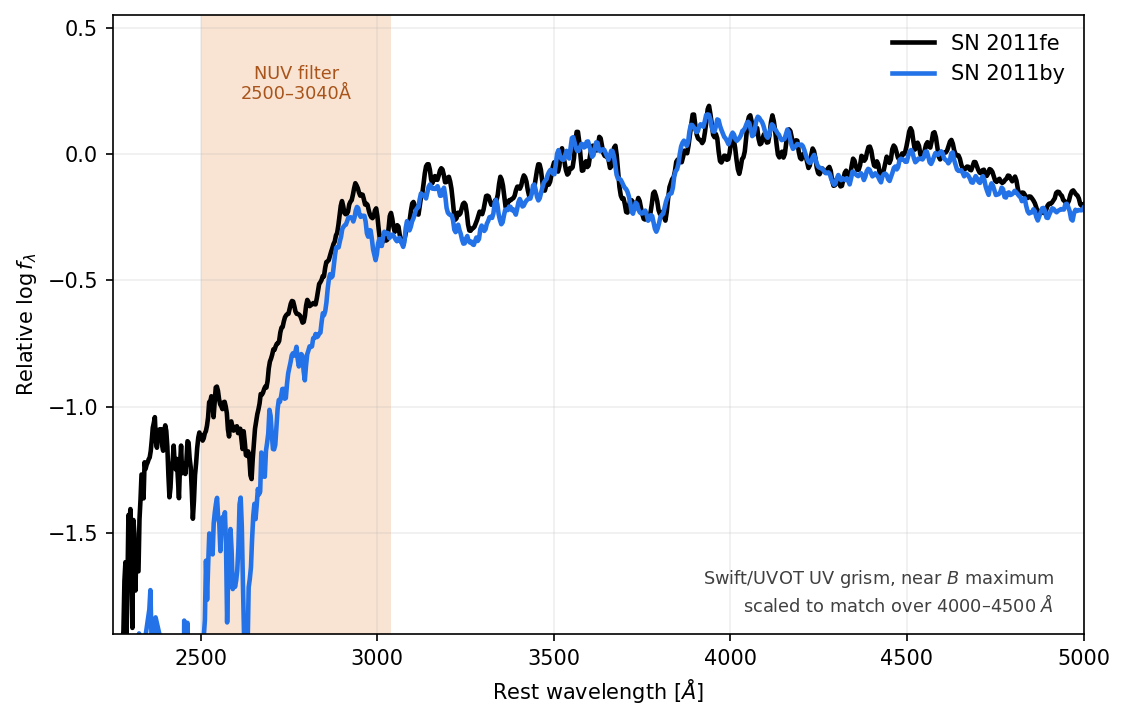
\includegraphics[width=0.62\textwidth]{snia_uvtwins.png}
\caption{Observed rest-frame UV--optical spectra of the optical twins SN\,2011fe (black) and SN\,2011by (blue), flux-calibrated Swift/UVOT UV-grism observations within half a day of $B$ maximum, from the Open Supernova Catalog archive \cite{guillochon2017}, deredshifted and scaled to match over $4000$--$4500$\,\AA. The shaded band marks the proposed rest-frame NUV filter ($2500$--$3040$\,\AA\ around the $2770$\,\AA\ diagnostic wavelength of Figure~\ref{fig:snuvlimit}). The optical region is nearly identical while the flux diverges strongly across that band, the near-ultraviolet metallicity signature of Foley \& Kirshner \cite{foleykirshner2013} predicted by Lentz et~al.\ \cite{lentz2000}. The optical twin condition isolates an intrinsic-luminosity difference visible \emph{only} in the rest-frame NUV \cite{graham2015}.}
\label{fig:uvtwins}
\end{figure}

Physically, the rest-frame NUV ($\lambda\lesssim3500$\,\AA) is dominated by a dense forest of iron-group element (IGE) lines such as Fe\,\textsc{ii}, Fe\,\textsc{iii}, Co\,\textsc{ii}, and Ni\,\textsc{ii}, whose blanketing is sensitive to three quantities. First, the total $^{56}$Ni mass, which sets the peak luminosity through $^{56}$Ni\,$\to^{56}$Co\,$\to^{56}$Fe. Second, the \emph{radial distribution} of IGE in the ejecta, which sets the opacity structure and the emergent UV flux. Third, the progenitor metallicity, which fixes the initial abundance of \emph{stable} iron-peak species ($^{54}$Fe, $^{58}$Ni) that blanket the UV without changing the radioactive budget \cite{lentz2000}. Two SNe Ia can therefore share an optical spectrum, set by intermediate-mass elements (Si, S, Ca) in the outer ejecta while differing in NUV flux set by IGE in the inner ejecta. Swift/UVOT photometry confirms that normal SNe Ia separate into NUV-red and NUV-blue subgroups offset by $\sim0.4$\,mag in NUV$-$optical color and crucially that the \emph{fraction} of each subgroup evolves with redshift \cite{milne2015}. A redshift-dependent subgroup mixture is exactly the kind of systematic that can bias $H_0$ and mimic or mask an evolving dark-energy equation of state.

\subsubsection{Rest-Frame NUV Access with a 0.36--3.0\,$\mu$m Slitless Survey}

The iron-group diagnostic normally requires a dedicated space-ultraviolet facility, because the rest-frame NUV is inaccessible from the ground and lies blueward of this mission's $0.36\,\mu$m cutoff at $z=0$. Redshift removes the obstacle. It shifts the iron-blanketing region \emph{into} the observed band. Figure~\ref{fig:nuvband} shows the mapping. The rest-frame $2500$\,\AA\ feature reaches the $0.36\,\mu$m blue edge already at $z\simeq0.44$, the $2500$--$3500$\,\AA\ core of the iron-blanketing region is in band by $z\simeq0.5$, and the full $2000$--$3500$\,\AA\ window enters by $z\simeq0.8$. The entire optical-twin baseline ($3500$--$7500$\,\AA) remains in band out to $z\simeq3$. The same diagnostic that demands a UV telescope at $z\approx0$ thus becomes accessible from this mission precisely in the $0.5\lesssim z\lesssim1.5$ regime where the time-domain tier already classifies SNe Ia.

\begin{figure}[tp]
\centering
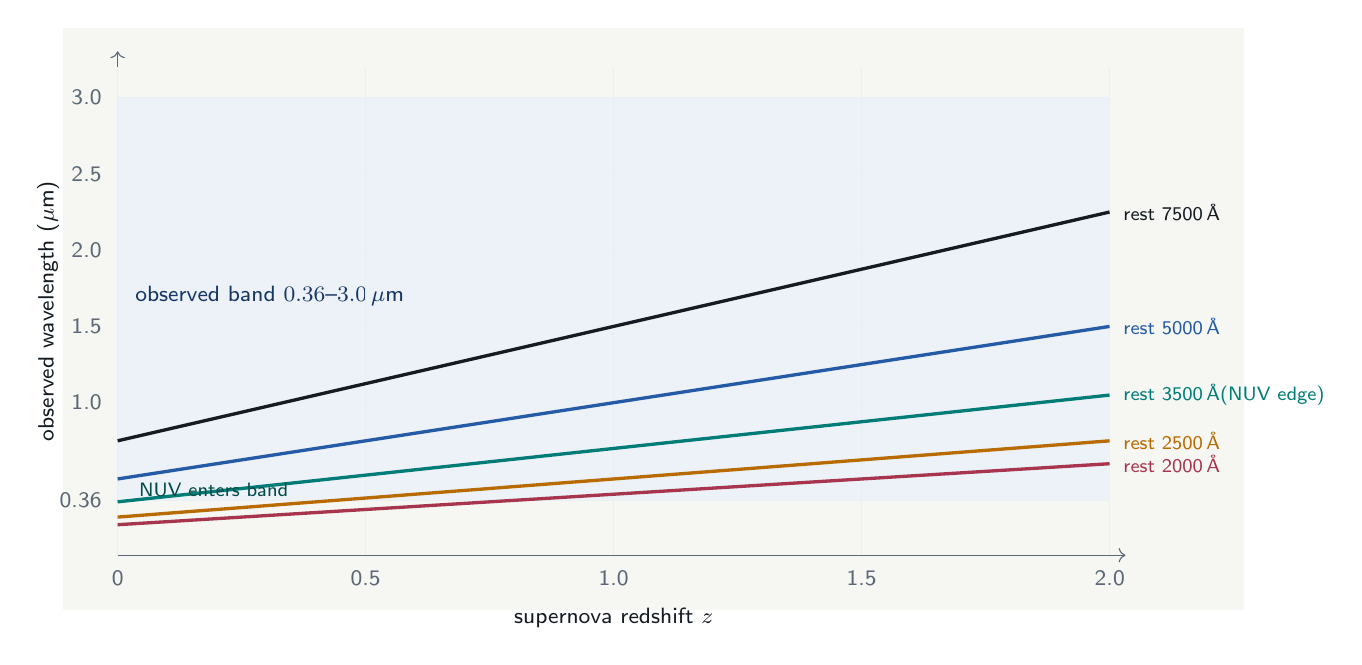
\begin{tikzpicture}[font=\sffamily\footnotesize]
  \def\w{12.6}\def\h{6.2}
  \def\zmax{2.0}\def\lmax{3.2}
  % axes mapping: x = z/zmax*w ; y = lambda_um/lmax*h
  \fill[paper] (-0.7,-0.7) rectangle (\w+1.7,\h+0.5);
  % observed band shading 0.36--3.0 um
  \fill[blue!8] (0,{0.36/\lmax*\h}) rectangle (\w,{3.0/\lmax*\h});
  \node[anchor=west,color=blue!60!black] at (0.1,{1.7/\lmax*\h}) {observed band $0.36$--$3.0\,\mu$m};
  \draw[->,color=muted] (0,0) -- (\w+0.2,0);
  \draw[->,color=muted] (0,0) -- (0,\h+0.2);
  \foreach \z in {0,0.5,1.0,1.5,2.0} {
    \pgfmathsetmacro\xx{\z/\zmax*\w}
    \draw[line!55] (\xx,0) -- (\xx,\h);
    \node[anchor=north,color=muted] at (\xx,-0.08) {\z};}
  \foreach \l/\lab in {0.36/0.36,1.0/1.0,1.5/1.5,2.0/2.0,2.5/2.5,3.0/3.0} {
    \pgfmathsetmacro\yy{\l/\lmax*\h}
    \draw[line!45] (0,\yy) -- (\w,\yy);
    \node[anchor=east,color=muted] at (-0.08,\yy) {\lab};}
  % redshifted rest lines: lambda_obs = lambda_rest*(1+z)
  % rest 2000 (NUV blue), 2500, 3500 (NUV red edge), 5000, 7500 (optical red)
  \foreach \lr/\col/\name/\ly in {0.2/rose/{rest 2000\,\AA}/0.0, 0.25/gold/{rest 2500\,\AA}/0.0, 0.35/teal/{rest 3500\,\AA (NUV edge)}/0.0, 0.5/blue/{rest 5000\,\AA}/0.0, 0.75/ink/{rest 7500\,\AA}/0.0} {
    \draw[\col,line width=1.2pt] plot[domain=0:\zmax,samples=40] ({\x/\zmax*\w},{min(\lr*(1+\x),\lmax)/\lmax*\h});
    \pgfmathsetmacro\yend{min(\lr*(1+\zmax),\lmax)/\lmax*\h}
    \node[anchor=west,color=\col,font=\sffamily\scriptsize] at (\w+0.05,\yend) {\name};}
  % mark NUV entry at z=0.5 for 3500 -> 0.36? actually 2500*(1+0.44)=3600
  \node[anchor=north,color=ink] at (0.5*\w,-0.55) {supernova redshift $z$};
  \node[rotate=90,anchor=south,color=ink] at (-0.62,0.5*\h) {observed wavelength ($\mu$m)};
  \node[anchor=west,color=teal!60!black,font=\sffamily\scriptsize] at (0.15,{0.43/\lmax*\h}) {NUV enters band};
\end{tikzpicture}
\caption{How redshift brings the rest-frame iron-group diagnostic into the observed band. Each colored curve is a fixed rest-frame wavelength shifted as $\lambda_{\rm obs}=\lambda_{\rm rest}(1+z)$. The shaded region is the proposed $0.36$--$3.0\,\mu$m coverage. The rest-frame NUV iron-blanketing window ($2000$--$3500$\,\AA) enters the band progressively with its $2500$\,\AA\ core crossing near $z\simeq0.44$ and the full window in band by $z\simeq0.8$, while the optical-twin baseline ($3500$--$7500$\,\AA) stays in band to $z\simeq3$. In the mission's working range $0.5\lesssim z\lesssim1.5$ a single multi-roll slitless spectrum records both the optical light-curve parameters and the rest-NUV iron-group color.}
\label{fig:nuvband}
\end{figure}

This diagnostic is within reach of the baseline spectrograph and is \emph{not} resolution-limited. SN Ia features are intrinsically broad. Photospheric-phase P\,Cygni lines have velocity widths of $\sim$$10^4$\,\kms, equivalent to an effective resolution of only $R\sim c/v\sim30$. The rest-frame NUV iron-group signature is a still broader pseudo-continuum suppression rather than a set of narrow lines. The native $R=1000$ therefore over-resolves the relevant structure by more than an order of magnitude. The analysis can bin down to $R\simeq100$--300 to accumulate signal-to-noise without erasing any diagnostic information. The limiting factor for $\Delta\mathrm{NUV}$ and $\theta_{\rm Fe}$ is blue-end signal-to-noise at the redshifted iron-blanketing wavelengths, not spectral resolution. The measurement is therefore feasible with the as-designed instrument and is governed by the same exposure-time reach shown in Figure~\ref{fig:snreach}. A single multi-roll slitless spectrum binned to $R\simeq300$--500 therefore records both the optical light-curve parameters and the rest-frame NUV iron-group color in one observation, enabling a subclass-aware standardization,
\begin{equation}
M_B = M_0 + \alpha\,(\Delta m_{15}-1.1) + \beta\,(B-V) + \gamma\,\Delta\mathrm{NUV} + \delta\,\theta_{\rm Fe},
\label{eq:nuvstd}
\end{equation}
where $\Delta\mathrm{NUV}$ is the rest-frame NUV color excess and $\theta_{\rm Fe}$ parameterizes the iron-group blanketing inferred from the spectrum. Adding these terms targets a reduction of the Hubble residual scatter from $\sigma\simeq0.12$\,mag toward $\sigma\lesssim0.08$\,mag, an $\sim30\%$ gain in per-object distance precision. This target is a design goal motivated by the reasoning above, not a result measured from an existing NUV spectroscopic sample. No survey has yet obtained rest-frame NUV spectra for a Hubble-flow SN Ia sample large enough to measure the achieved scatter reduction directly, and the true gain could be smaller if progenitor metallicity is only one of several unmodeled sources of scatter. It also lets the program test directly whether progenitor-metallicity evolution imprints a redshift-dependent standardization bias. Because the same explosion physics that drives the NUV divergence also sets the host-mass step, the spectroscopic $\theta_{\rm Fe}$ offers a physical replacement for the purely empirical host corrections used today.

\subsubsection{Observing Strategy and Survey Reach}

The central observational systematic is host-galaxy contamination, since the supernova trace is dispersed on top of the host light at the same sky position. Three properties of the program keep it controllable. First, the time-domain field is revisited on a fixed cadence. The supernova-free epochs therefore stack into a deep host-only dispersed template whose subtraction isolates the transient spectrum, the dispersed-domain counterpart of the image subtraction standard in ground-based supernova photometry. The template is far deeper than any single visit. Hence, the subtraction noise is dominated by the supernova epoch itself. Second, the supernova is an unresolved point source. Its trace stays sharp at two pixels per resolution element, while the host light is smeared by the host size into a smooth background of much lower effective resolution (Section~\ref{sec:effres}). What competes with the supernova is the host surface brightness at the supernova position rather than the total host magnitude. Third, Roman slitless simulations motivate three-dimensional host-scene reconstruction from multi-roll spectroscopy before subtracting host light from supernova spectra \cite{astraatmadja2026}. The same three-orientation strategy required by the flagship ELG survey supplies exactly this capability for the time-domain field. The approach is also flight-proven. HST classified its $z>1$ GOODS supernovae with the ACS grism, including SN\,2002fw at $z=1.3$ observed near maximum light \cite{riess2004}. The Roman reference time-domain survey adopts slitless prism spectroscopy for an expected $\sim$12{,}000 SNe Ia \cite{rose2021roman}. This proposal therefore claims a strong high-redshift SN standardization and physical-typing program, not a standalone sub-percent $H_0$ measurement.

For a normal SN Ia with $M_B\simeq-19.3$, the approximate peak magnitude is $m\simeq\mu(z)-19.3$ before bandpass, stretch, color, and host corrections. Here $\mu(z)$ is the distance modulus, set by the luminosity distance $d_L(z)$,
\begin{equation}
\mu(z)=5\log_{10}\!\left[\frac{d_L(z)}{10\,\mathrm{pc}}\right]=25+5\log_{10}\!\left[\frac{d_L(z)}{\mathrm{Mpc}}\right],
\qquad
d_L(z)=\frac{c\,(1+z)}{H_0}\int_0^z\frac{dz'}{E(z')},
\label{eq:distmod}
\end{equation}
with $E(z)=\big(\Omega_m(1+z)^3+(1-\Omega_m)(1+z)^{3(1+w)}\big)^{1/2}$ for a flat model of dark-energy equation of state $w$, reducing to $E(z)=\big(\Omega_m(1+z)^3+\Omega_\Lambda\big)^{1/2}$ for $\Lambda$CDM. Because $d_L\propto H_0^{-1}$, the distance modulus includes an additive $-5\log_{10}H_0$ term. Therefore, raising $H_0$ shifts the entire Hubble diagram brighter (toward smaller $\mu$) by $5\log_{10}(H_0/H_0')$\,mag, a pure vertical offset. The \emph{shape} of $\mu(z)$ with redshift, by contrast, is fixed by $\Omega_m$ and the dark-energy parameters and is independent of $H_0$. At low redshift this expands to the Hubble law $\mu\simeq25+5\log_{10}\!\big(cz/H_0\,[\mathrm{Mpc}]\big)+1.086\,(1-q_0)\,z+\cdots$, with $q_0=\tfrac12\Omega_m(1+3w)+\cdots$ the deceleration parameter. A binned slitless spectrum reaching $m_{\rm AB}\simeq24.5$ in 2 hr can classify normal SN Ia to $z\simeq0.9$ near peak. In 10 hr it reaches $m_{\rm AB}\simeq25.4$ and $z\simeq1.25$. In 30 hr it reaches $m_{\rm AB}\simeq26.0$ and $z\simeq1.5$ for favorable events (Figure~\ref{fig:snreach}). These are planning values for spectra binned to $R\simeq300$--500 after combining three orientations. The rest-NUV diagnostic of Eq.~\eqref{eq:nuvstd} is signal-limited at the blue end. Hence, the iron-group color is most robustly measured for the brighter, lower-redshift half of each tier, while classification and host-redshift control extend across the full reach.

\begin{figure}[tp]
\centering
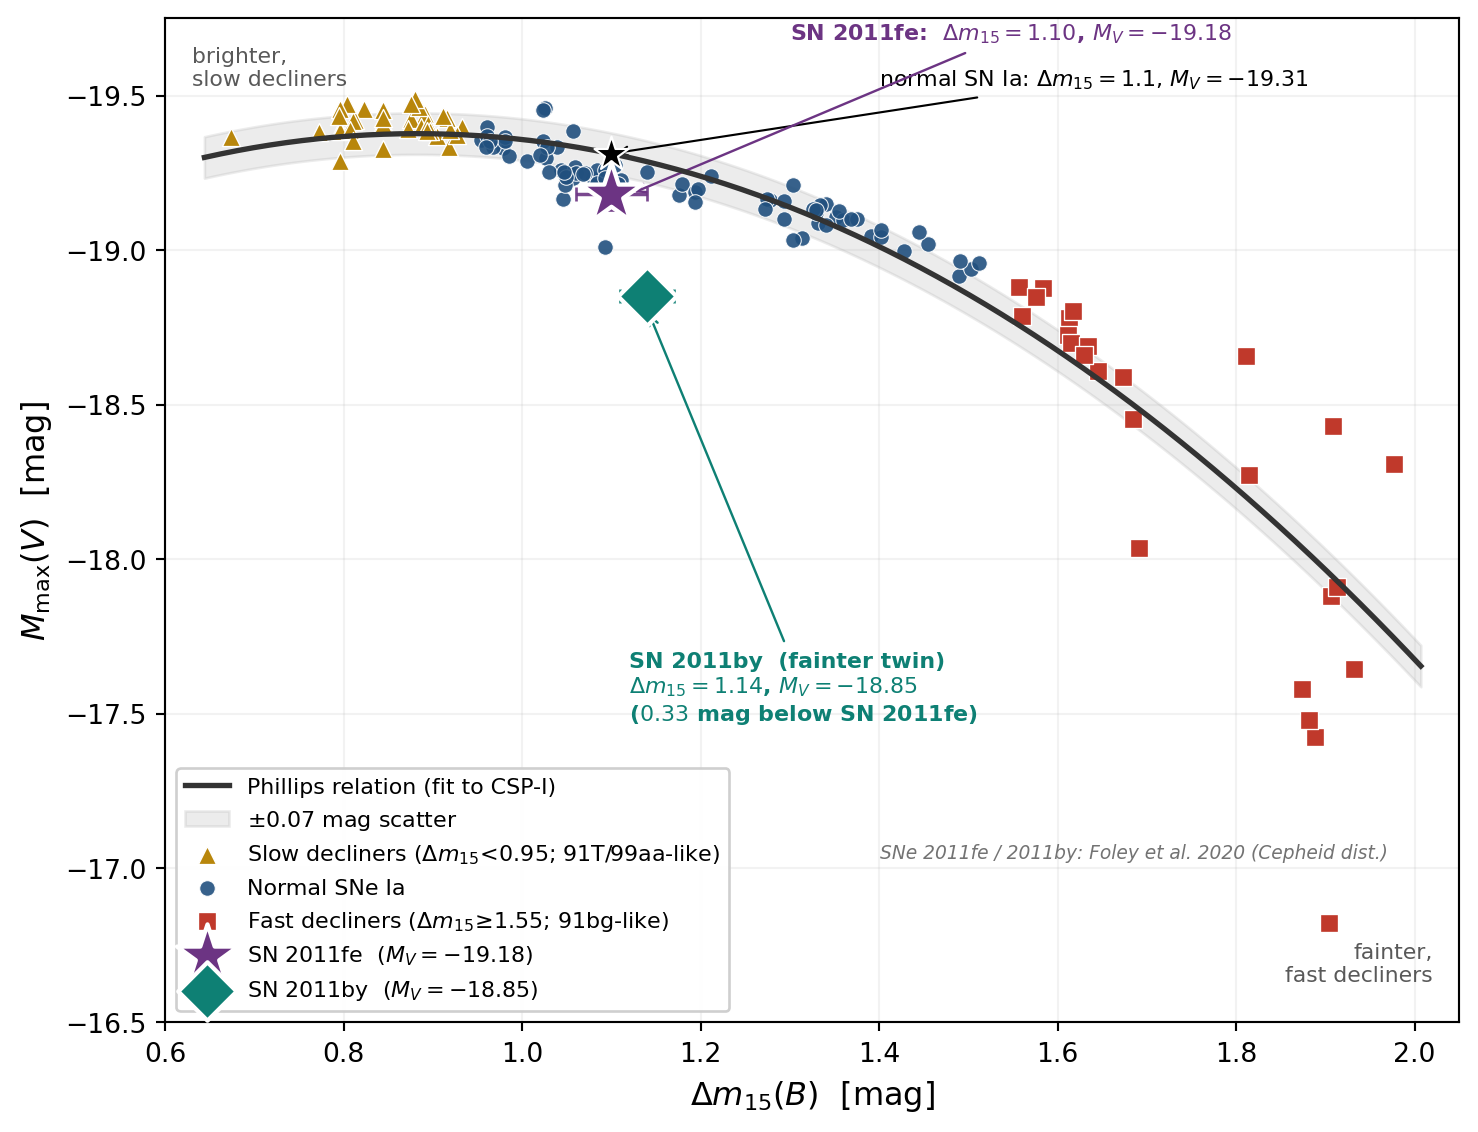
\includegraphics[width=0.72\textwidth]{phillips_relation.png}
\caption{The Phillips width--luminosity relation which underpins SN Ia standardization, built from the real Carnegie Supernova Project\,I sample (139 SNe Ia; Burns et al.\ \cite{burns2018csp}) and presented in the style of Figure 11 of Zeng et al.\ \cite{zeng2025sn2023ehl}. The peak absolute $V$ magnitude $M_{\max}(V)$, corrected for host-galaxy extinction with the per-SN reddening and $R_V$ tabulated by the survey, is plotted against the post-maximum decline rate $\Delta m_{15}(B)$, so that brighter supernovae decline more slowly. The solid curve is a quadratic fit to these data, passing through $M_V=-19.31$ at $\Delta m_{15}=1.1$ with a residual scatter of $0.07$\,mag, shown as the shaded band. Points are coloured by decline-rate regime, the physical axis along which the recognized subtypes separate, namely the slow-declining over-luminous 1991T/1999aa-like events, normal SNe Ia, and the fast-declining sub-luminous 1991bg-like events. A single light-curve-shape parameter captures most, but not all, of the luminosity diversity, and the residual structure is the systematic that rest-frame NUV spectroscopy is designed to diagnose. The CSP absolute scale adopts $H_0=72$\,\kms\,Mpc$^{-1}$, which fixes only the zero-point, not the shape, of the relation.}
\label{fig:phillips}
\end{figure}

\begin{figure}[tp]
\centering
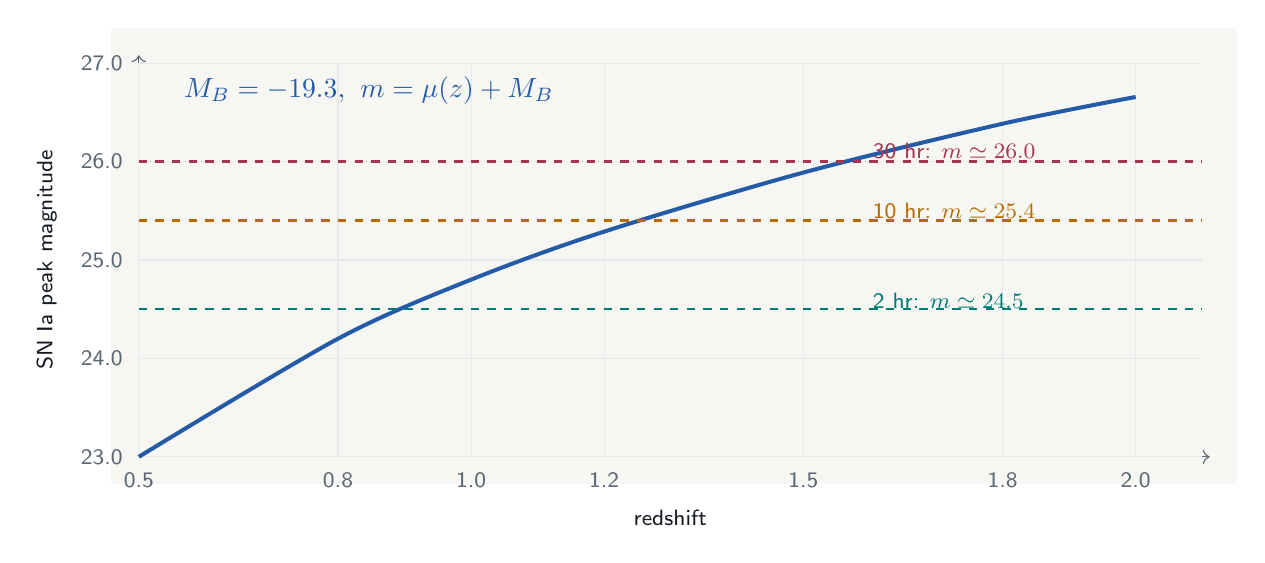
\begin{tikzpicture}[font=\sffamily\footnotesize]
  \def\w{13.5}
  \def\h{5.0}
  \fill[paper] (-0.35,-0.35) rectangle (\w+0.45,\h+0.45);
  \draw[->,color=muted] (0,0) -- (\w+0.1,0);
  \draw[->,color=muted] (0,0) -- (0,\h+0.1);
  \foreach \x/\lab in {0/0.5,2.53/0.8,4.22/1.0,5.91/1.2,8.44/1.5,10.97/1.8,12.66/2.0} {
    \draw[line!65] (\x,0) -- (\x,\h);
    \node[anchor=north,color=muted] at (\x,-0.08) {\lab};
  }
  \foreach \y/\lab in {0/23.0,1.25/24.0,2.5/25.0,3.75/26.0,5.0/27.0} {
    \draw[line!65] (0,\y) -- (\w,\y);
    \node[anchor=east,color=muted] at (-0.08,\y) {\lab};
  }
  \draw[blue,line width=1.45pt,smooth]
    plot coordinates {(0,0.0) (2.53,1.50) (4.22,2.25) (5.91,2.86) (8.44,3.61) (10.97,4.23) (12.66,4.57)};
  \draw[teal,line width=0.9pt,dashed] (0,1.875) -- (\w,1.875);
  \draw[gold,line width=0.9pt,dashed] (0,3.0) -- (\w,3.0);
  \draw[rose,line width=0.9pt,dashed] (0,3.75) -- (\w,3.75);
  \node[anchor=west,color=teal] at (9.2,1.98) {2 hr: $m\simeq24.5$};
  \node[anchor=west,color=gold] at (9.2,3.12) {10 hr: $m\simeq25.4$};
  \node[anchor=west,color=rose] at (9.2,3.88) {30 hr: $m\simeq26.0$};
  \node[anchor=north,color=ink] at (0.5*\w,-0.55) {redshift};
  \node[rotate=90,anchor=south,color=ink] at (-0.92,0.5*\h) {SN Ia peak magnitude};
  \node[anchor=west,color=blue,font=\bfseries] at (0.45,4.65) {$M_B=-19.3,\ m=\mu(z)+M_B$};
\end{tikzpicture}
\caption{Planning reach for binned $R\simeq300$--500 SN Ia slitless spectra. The exposure labels are total science time after combining the three required orientations.}
\label{fig:snreach}
\end{figure}

An independent first-principles check with the exposure-time calculator confirms this reach and quantifies the rest-ultraviolet access. Using the Nugent Type Ia template at peak normalised to $M_B=-19.3$, Figure~\ref{fig:sniamag} gives the observed magnitude in each band as a function of redshift. Figure~\ref{fig:sniamuv} follows the rest-frame near-ultraviolet diagnostic near $2770$\,\AA, which the band captures for $z\gtrsim0.3$. The calculator reaches the rest-NUV of a peak Type Ia in minutes to $z\simeq2$. Therefore, the near-ultraviolet divergence that separates the optical twins is measurable across the redshift range that anchors the distance scale.

\begin{figure}[tp]
\centering
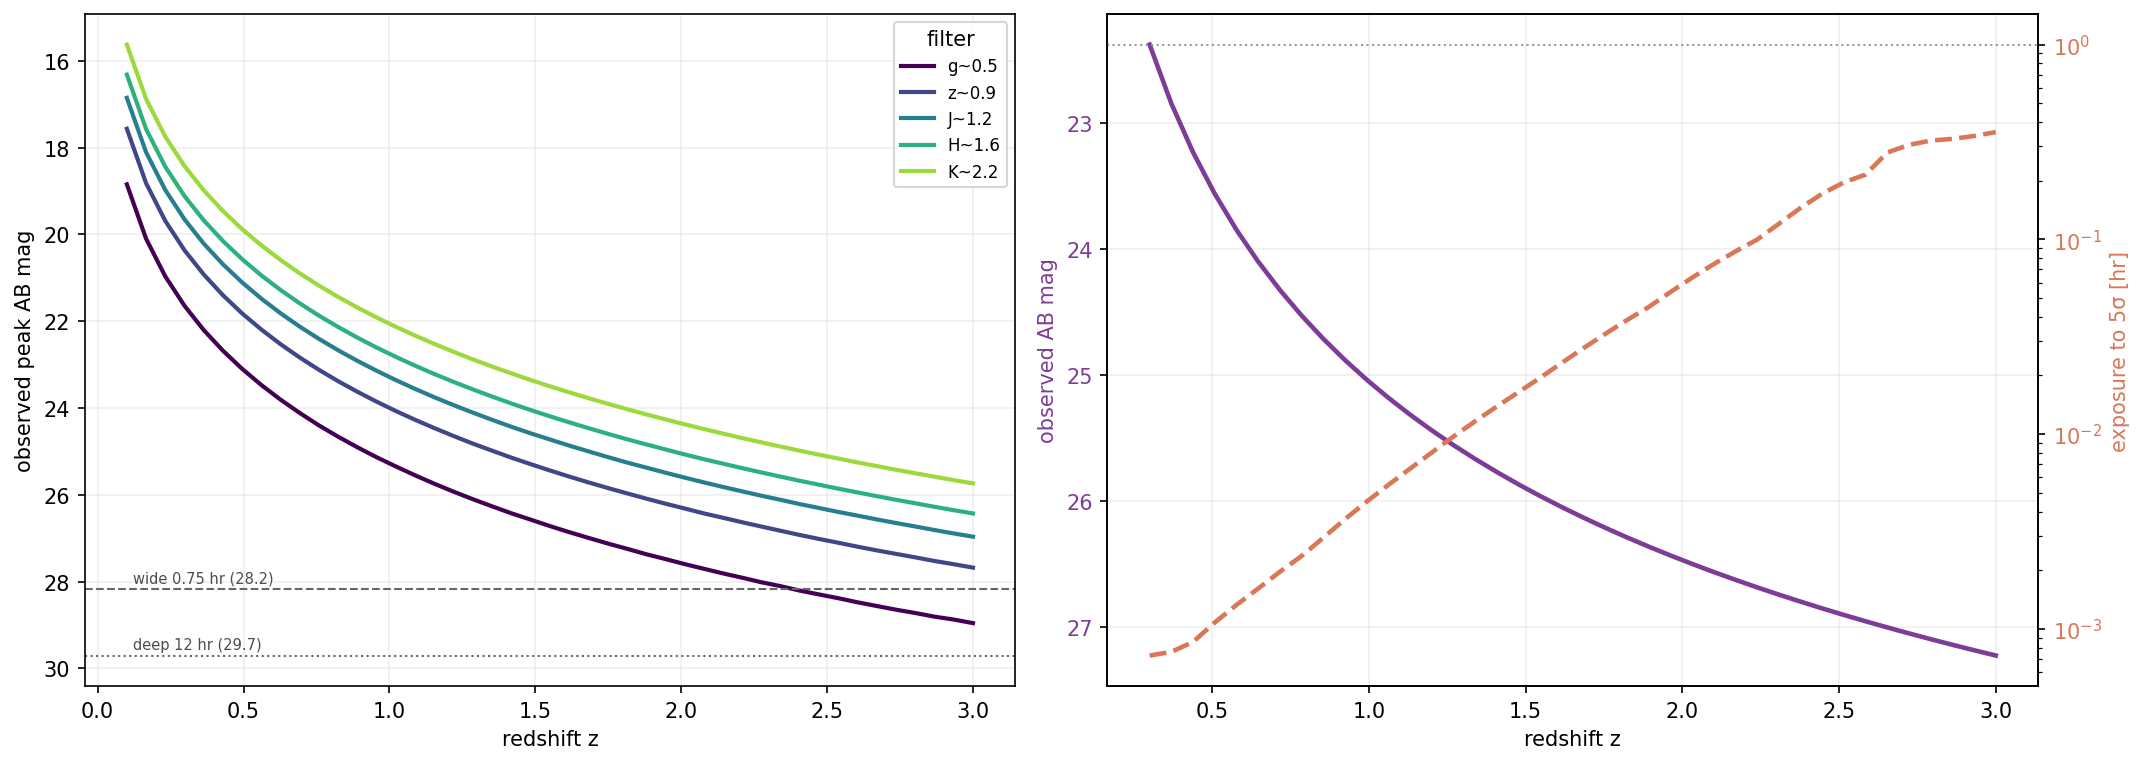
\includegraphics[width=\textwidth]{snia_demo_combined.png}
\caption{\emph{Left}: Type Ia SN at peak ($M_B=-19.3$, Nugent template) observed AB magnitude per band versus redshift for the $3.5$\,m concept with the wide ($0.75$\,hr) and deep ($12$\,hr) $H$-band point-source depths marked. The redder bands hold the peak above the wide depth to $z\gtrsim2$. \emph{Right}: the rest-frame near-ultraviolet ($2770$\,\AA) of a peak Type Ia as it redshifts into the band. Left axis, observed AB magnitude. Right axis, exposure to a $5\sigma$ detection. The rest-NUV twin diagnostic is reached in minutes to $z\simeq2$.}
\label{fig:sniamag}
\label{fig:sniamuv}
\end{figure}

\subsubsection{The S/N-Limited Redshift of the Twin \texorpdfstring{$U$}{U} and NUV Photometry}

The $5\sigma$ detection reach of Figure~\ref{fig:sniamuv} is not the right requirement for the twin program, because the twin diagnostic is a magnitude rather than a detection. The NUV-red and NUV-blue subgroups are offset by $\sim0.4$\,mag in NUV$-$optical colour at matched optical light curves \cite{milne2015}. The optical side of that colour comes essentially free since the optical bands are one to two magnitudes brighter and, therefore, the colour error is the NUV magnitude error. Assigning a single supernova to a subgroup with the $0.4$\,mag offset resolved at $4\sigma$ therefore requires $\sigma_m\simeq0.10$\,mag in the rest-frame band, which through $\sigma_m=2.5/(\ln 10\cdot {\rm S/N})$ means ${\rm S/N}\simeq11$. Using $\Delta{\rm NUV}$ as the continuous standardization covariate of Eq.~\eqref{eq:nuvstd} at the $\sigma\lesssim0.08$\,mag Hubble-residual target requires $\sigma_m\simeq0.05$\,mag, or ${\rm S/N}\simeq22$.

Figure~\ref{fig:snuvlimit} computes where those thresholds are met, using the exposure-time calculator in its slitless mode with the Nugent peak template at $M_B=-19.3$. Synthetic rest-frame top-hat filters, $U$ at $3300$--$3900$\,\AA\ and NUV at $2500$--$3040$\,\AA\ around the $2770$\,\AA\ diagnostic wavelength, are redshifted with the source. The filter magnitude is measured by binning the multi-roll slitless spectrum over the redshifted band, with the dispersed zodiacal, cirrus, and thermal sky of the band-limiting filter, dark current, and read noise included in the budget. The NUV filter clears the $0.36\,\mu$m blue edge completely at $z\geq0.44$ and the $U$ filter already at $z\geq0.09$. Therefore, the $U$ magnitude bridges the low-redshift range where the NUV is not yet in band. At the $2$\,hr classification depth the subgroup assignment ($\sigma_m=0.10$) holds to $z\simeq0.86$ in the NUV and $z\simeq1.06$ in $U$, while covariate-grade photometry ($\sigma_m=0.05$) holds to $z\simeq0.55$ and $0.75$ respectively. The $10$\,hr tier extends subgroup assignment to $z\simeq1.28$ (NUV) and $1.54$ ($U$) and covariate-grade measurement to $z\simeq0.90$ and $1.12$. The $30$\,hr stacks reach $z\simeq1.71$ in the NUV. The flattening of the $U$ curves near $z\simeq1.8$ marks the band crossing the $1\,\mu$m dichroic onto the near-infrared arm, where the zodiacal sky is darkest. The S/N-limited redshift of the twin photometry therefore sits at $z\simeq0.9$--$1.3$ for the survey's standard exposures, squarely covering the $0.5\lesssim z\lesssim1.5$ range where the time-domain tier classifies its supernovae. The covariate-grade half of each tier is exactly the ``brighter, lower-redshift half'' anticipated in the observing strategy above. These redshift reaches are read directly off the idealised slitless calculator without a survey-depth anchor, so, per the margin quantified in Section~\ref{sec:etc}, they should be read as an upper bound that a fielded pipeline will likely fall somewhat short of.

\begin{figure}[tp]
\centering

\includegraphics[width=\textwidth]{snia_uvnuv_zlimit.png}
\caption{The S/N-limited redshift of the SN Ia rest-frame $U$ (left) and NUV (right) filter photometry from the slitless exposure-time calculator for a peak normal SN Ia ($M_B=-19.3$, Nugent template). Each curve gives the exposure at which the synthetic filter magnitude reaches $\sigma_m=0.10$\,mag (solid, the $4\sigma$ NUV-red/NUV-blue subgroup assignment \cite{milne2015}) and $\sigma_m=0.05$\,mag (dashed, covariate-grade photometry, Eq.~\eqref{eq:nuvstd}). Dotted lines mark the $2$, $10$, and $30$\,hr planning exposures. The vertical dashed line marks where each filter clears the $0.36\,\mu$m blue edge. Subgroup classification reaches $z\simeq0.86$ (NUV) and $1.06$ ($U$) in $2$\,hr and $z\simeq1.28$ and $1.54$ in $10$\,hr.}
\label{fig:snuvlimit}
\end{figure}

\subsubsection{Cosmological Payoff: \texorpdfstring{$H_0$}{H0} Tension and Dynamic Dark Energy}

The motivation for a physically refined standardization is the precision now demanded by the two leading cosmological questions, both of which the SN Ia Hubble diagram addresses (Figure~\ref{fig:sniacosmo}). The first is the Hubble tension, the $\sim5\sigma$ discrepancy between the local determination ($H_0=73.04\pm1.04$\,\kms\,Mpc$^{-1}$, SH0ES \cite{riess2022}) and the CMB-inferred value ($67.4\pm0.5$\,\kms\,Mpc$^{-1}$, Planck \cite{planck2018}), a split now reproduced across many independent methods (Figure~\ref{fig:h0tension}). A significant share of the local error budget originates in the SN Ia standardization step. If NUV-red/NUV-blue subclasses with different luminosities are mixed in unequal proportions between the calibrator and Hubble-flow samples, $H_0$ is biased. A subclass-homogeneous, $\theta_{\rm Fe}$-aware ladder built from rest-NUV spectroscopy quantifies and removes this term, providing a cleaner local distance scale.

\begin{figure}[tp]
\centering

\includegraphics[width=0.76\textwidth]{h0_tension.png}
\caption{The Hubble tension shown as a compilation of $H_0$ determinations with the measured value on the horizontal axis and one method per row. Early-Universe probes calibrated on the sound horizon (blue squares: Planck CMB \cite{planck2018}, ACT$+$WMAP, SPT-3G, and BAO$+$BBN) cluster near $67.4\pm0.5$\,\kms\,Mpc$^{-1}$, whereas late-Universe direct and distance-ladder probes (red circles: SH0ES Cepheids$+$SN\,Ia \cite{riess2022}, TRGB, JWST multi-method, surface-brightness fluctuations, megamasers, Miras, Tully--Fisher, and time-delay lensing) cluster near $73\pm1$\,\kms\,Mpc$^{-1}$. The shaded bands mark the Planck and SH0ES anchors, whose central values differ by $5.7$\,\kms\,Mpc$^{-1}$ ($\approx4.8\sigma$ for these two alone and $\sim5\sigma$ for the full early-versus-late split). A subclass-homogeneous, iron-group-aware SN\,Ia ladder built from rest-NUV spectroscopy attacks the dominant astrophysical term in the late-Universe column.}
\label{fig:h0tension}
\end{figure}

The second is the dark-energy equation of state. Unrecognized astrophysical systematics in the Hubble diagram can mimic or mask dynamic dark energy. As Figure~\ref{fig:sniacosmo} shows, distinguishing $\Lambda$CDM from a CPL model with $(w_0,w_a)$ deviations requires sub-$0.1$-mag control of the residuals. This is below the current per-SN scatter and only reached with the NUV-augmented calibration of Eq.~\eqref{eq:nuvstd}. Because this mission also delivers the flagship ELG BAO/RSD measurements, the SN Ia distances and the BAO standard ruler can be combined internally, together with external Planck/ACT CMB priors, into a joint constraint on $H_0$, $\Omega_m$, and $(w_0,w_a)$ with the SN systematic now physically controlled rather than marginalized.

\begin{figure}[tp]
\centering
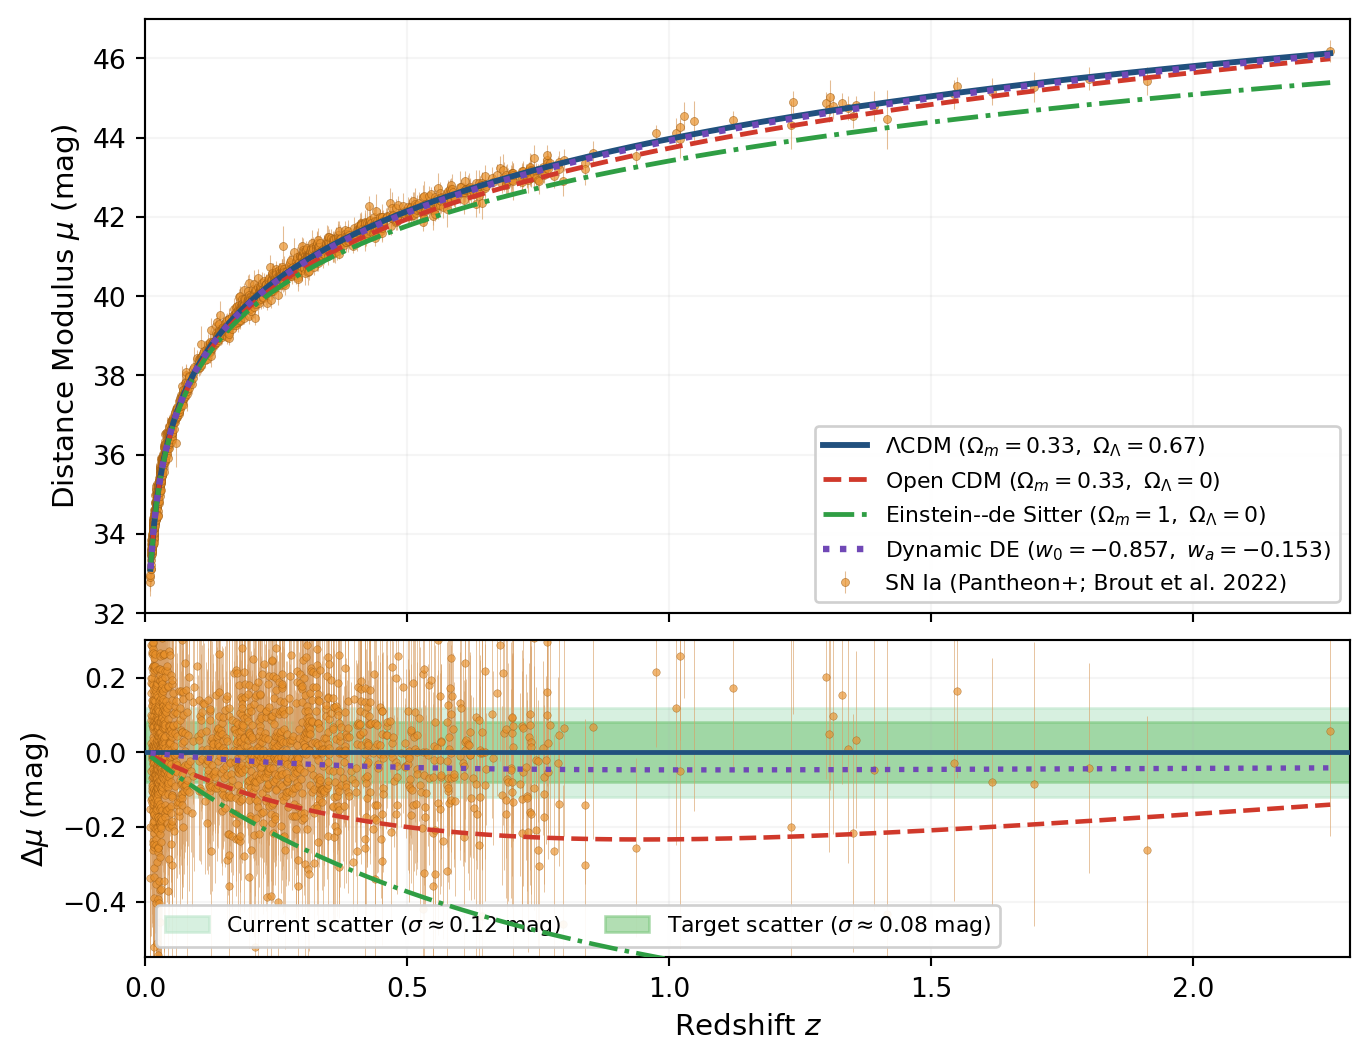
\includegraphics[width=0.76\textwidth]{snia_hubble_cosmologies.png}
\caption{SN Ia Hubble diagram and the precision required for dark-energy science. \emph{Upper:} distance modulus $\mu$ versus redshift for the real Pantheon$+$SH0ES sample (1580 Hubble-flow SNe Ia, Cepheid calibrators removed; Brout et~al.\ \cite{brout2022}) against four cosmologies, namely $\Lambda$CDM ($\Omega_m=0.33$, $\Omega_\Lambda=0.67$), open CDM, Einstein--de\,Sitter, and a CPL dynamic dark-energy model ($w_0=-0.857$, $w_a=-0.153$). The reference cosmology uses the Pantheon$+$ flat-$\Lambda$CDM best fit ($H_0=73.04$, $\Omega_m=0.334$). \emph{Lower:} residuals $\Delta\mu$ relative to $\Lambda$CDM. The shaded bands show the current per-SN scatter ($\sigma\approx0.12$\,mag) and the target after the NUV-augmented calibration of Eq.~\eqref{eq:nuvstd} ($\sigma\approx0.08$\,mag). Separating $\Lambda$CDM from dynamic dark energy requires sub-$0.1$-mag control, motivating the iron-group-aware standardization enabled by rest-frame NUV access.}
\label{fig:sniacosmo}
\end{figure}

The SN Ia program therefore extends beyond classification and redshift service. By reaching the rest-frame NUV of $0.5\lesssim z\lesssim1.5$ supernovae it can diagnose the iron-group physics that sets the dominant intrinsic-luminosity systematic, convert the empirical host-mass step into a physical correction, and feed a subclass-homogeneous high-redshift distance set into the same dark-energy analysis as the flagship BAO/RSD survey.

\subsection{Strong-Lens Cosmography}\label{sec:stronglens}

Strong gravitational lensing is a purely geometric cosmological probe. The deflection of light by a foreground mass depends on ratios of angular-diameter distances to the lens and the source. Hence, a measured lens configuration constrains the expansion history independently of, and with different systematics from, the BAO and supernova programs above. It therefore provides an independent check on $H_0$ and the dark-energy equation of state. The cosmological signal is entangled with the lens mass distribution through three well-known systematics. First, the \emph{mass-sheet degeneracy} (MSD), under which a rescaling of the convergence plus a uniform sheet leaves all observables except the absolute time delay unchanged. Second, the \emph{mass--anisotropy degeneracy} in the stellar dynamics used to break the MSD. Third, the \emph{external convergence} $\kappa_{\rm ext}$ from mass along the line of sight. A credible program is therefore defined by how well it controls these three terms, not by how many lenses it collects.

This mission does not rely primarily on its spectrograph for that task. The slitless design provides diffraction-limited, photometrically stable direct imaging ($\sim$0.1\,arcsec at optical wavelengths) which is the natural data product for lens finding and for reconstructing Einstein rings and arcs. Spectroscopy is a \emph{complement}. It supplies lens and source redshifts, deflector velocity dispersions, and line-of-sight galaxy redshifts, but it is not a prerequisite for the imaging-based core of the program. The strategy below therefore treats imaging $+$ machine learning as the engine with spectroscopy and (where useful) weak-lensing shapes as degeneracy-breaking add-ons. The next-generation imaging surveys will soon deliver lenses in large numbers. These include of order $1.7\times10^5$ discoverable galaxy--galaxy lenses in \textit{Euclid} and $1.2\times10^5$ in Rubin/LSST \cite{collett2015}, $\sim$$1.7\times10^4$ in the \textit{Roman} High-Latitude Survey \cite{weiner2020}, with \textit{Euclid} already publishing hundreds of space-based candidates over its first 63\,\degti\ and projecting $>10^5$ for the full survey \cite{walmsley2025}. Meanwhile, redshift confirmation \cite{shu2025} and per-lens mass modeling remain the rate-limiting steps.

\subsubsection{Primary Probe: Double-Source-Plane Lenses for \texorpdfstring{$w$}{w} and \texorpdfstring{$\Omega_m$}{Omega_m}}

The cleanest strong-lensing cosmology available to a spectroscopic-imaging mission is the \emph{double-source-plane lens} (DSPL), a single deflector lensing two background sources at distinct redshifts $z_{s1}<z_{s2}$ (Figure~\ref{fig:dspl}). The ratio of the two Einstein radii fixes the dimensionless distance ratio
\begin{equation}
\beta \;=\; \frac{D_{ds1}\,D_{s2}}{D_{s1}\,D_{ds2}},
\label{eq:dsplbeta}
\end{equation}
where $D_{s}$ and $D_{ds}$ are angular-diameter distances from observer and from deflector to each source. Because $\beta$ is a ratio of distances at a common lens, it is essentially \emph{independent of $H_0$} and of the absolute mass normalization and depends only on $\Omega_m$ and the dark-energy parameters. The archetype, the ``Jackpot'' lens SDSS\,J0946$+$1006, yields $\beta^{-1}=1.404\pm0.016$ and, combined with CMB priors in a flat $w$CDM model, $w=-1.17\pm0.20$, a $\sim$30\% improvement over the CMB alone \cite{collettauger2014}. Forecasts show that a handful of well-modeled DSPLs reach $\sigma(w)\approx0.15$ \cite{collett2012}. Recent AGEL-survey systems have begun to realize this, improving the $w$ precision by $\sim$30--40\% over CMB-only when combined \cite{sahu2025,bowden2025}.

DSPLs are rare and were historically found by accident, because identifying \emph{two} source redshifts behind one lens is hard from imaging alone. This is where the mission's combination of imaging and spectroscopy matters. The stable imaging resolves the two concentric ring/arc systems, measuring their radii, while the slitless spectroscopy delivers the two source redshifts and the lens redshift in the same observation, turning serendipitous discoveries into a systematically assembled DSPL cosmology sample. We adopt DSPL distance-ratio cosmography as the primary strong-lensing science goal because its dominant requirement, multiple secure source-plane redshifts, is exactly the measurement a wide-field spectroscopic survey makes naturally and because the $\beta$ ratio sidesteps both the $H_0$ calibration and much of the MSD which complicates time-delay work.

\begin{figure}[tp]
\centering
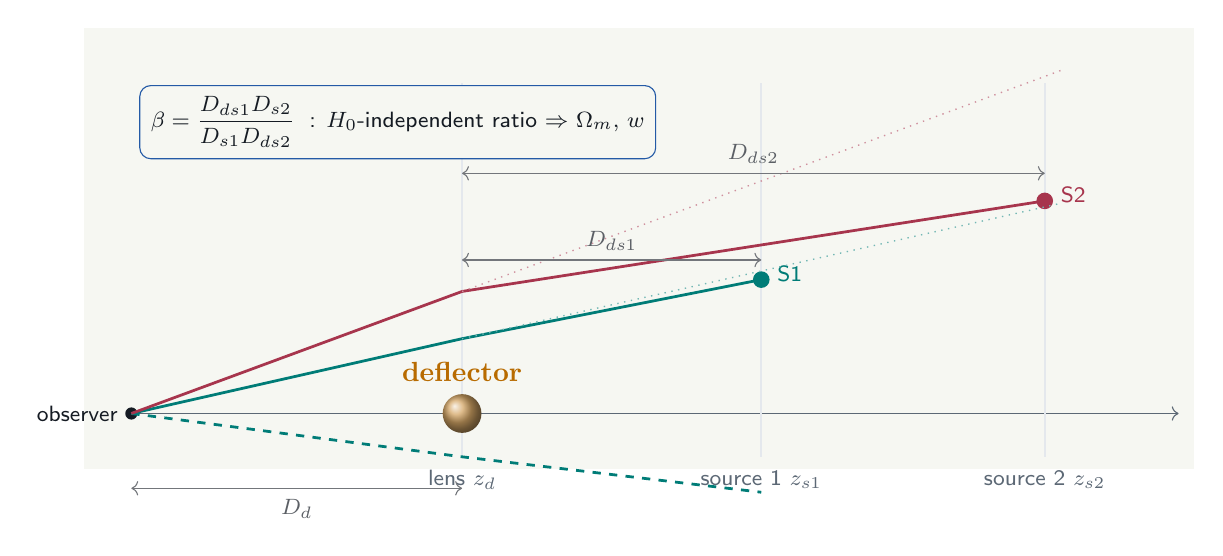
\begin{tikzpicture}[font=\sffamily\footnotesize]
  \def\xo{0}\def\xl{4.2}\def\xa{8.0}\def\xb{11.6}
  \def\h{4.2}
  \fill[paper] (-0.6,-0.7) rectangle (\xb+1.9,\h+0.7);
  % optical axis
  \draw[muted,->] (\xo,0) -- (\xb+1.7,0);
  % planes
  \draw[line!70,line width=0.8pt] (\xl,-0.55) -- (\xl,\h);
  \draw[line!70,line width=0.8pt] (\xa,-0.55) -- (\xa,\h);
  \draw[line!70,line width=0.8pt] (\xb,-0.55) -- (\xb,\h);
  \node[anchor=north,color=muted] at (\xl,-0.6) {lens $z_d$};
  \node[anchor=north,color=muted] at (\xa,-0.6) {source 1 $z_{s1}$};
  \node[anchor=north,color=muted] at (\xb,-0.6) {source 2 $z_{s2}$};
  % observer
  \fill[ink] (\xo,0) circle (2.2pt);
  \node[anchor=east,color=ink] at (\xo-0.05,0) {observer};
  % deflector
  \shade[ball color=gold!60] (\xl,0) circle (7pt);
  \node[anchor=south,color=gold,font=\bfseries] at (\xl,0.28) {deflector};
  % sources
  \fill[teal] (\xa,1.7) circle (3pt); \node[anchor=west,color=teal] at (\xa+0.08,1.78) {S1};
  \fill[rose] (\xb,2.7) circle (3pt); \node[anchor=west,color=rose] at (\xb+0.08,2.78) {S2};
  % bent rays for source 1 (upper image): obs -> lens(offset) -> S1
  \draw[teal,line width=1.0pt] (\xo,0) -- (\xl,0.95) -- (\xa,1.7);
  \draw[teal,line width=1.0pt,dashed] (\xo,0) -- (\xl,-0.55) -- (\xa,-1.0) coordinate(s1m);
  % bent rays for source 2: obs -> lens(larger offset) -> S2
  \draw[rose,line width=1.0pt] (\xo,0) -- (\xl,1.55) -- (\xb,2.7);
  % apparent image directions (thin extensions)
  \draw[teal!55,line width=0.5pt,dotted] (\xl,0.95) -- (\xb+0.2,{0.95/\xl*(\xb+0.2)});
  \draw[rose!55,line width=0.5pt,dotted] (\xl,1.55) -- (\xb+0.2,{1.55/\xl*(\xb+0.2)});
  % distance braces along axis
  \draw[ink!60,<->] (\xo,-0.95) -- (\xl,-0.95); \node[anchor=north,color=ink!70] at ({0.5*(\xo+\xl)},-0.97) {$D_d$};
  \draw[ink!60,<->] (\xl,1.95) -- (\xa,1.95); \node[anchor=south,color=ink!70] at ({0.5*(\xl+\xa)},1.95) {$D_{ds1}$};
  \draw[ink!60,<->] (\xl,3.05) -- (\xb,3.05); \node[anchor=south,color=ink!70] at ({0.5*(\xl+\xb)},3.05) {$D_{ds2}$};
  % beta box
  \node[anchor=west,draw=blue,fill=paper,rounded corners,inner sep=4pt,text=ink] at (0.1,3.7)
     {$\displaystyle \beta=\frac{D_{ds1}D_{s2}}{D_{s1}D_{ds2}}$ \;: $H_0$-independent ratio $\Rightarrow$ $\Omega_m,\,w$};
\end{tikzpicture}
\caption{Double-source-plane lens geometry. One deflector at $z_d$ lenses two sources at $z_{s1}$ (teal) and $z_{s2}$ (rose). The ratio of their Einstein radii fixes the distance ratio $\beta$ of Eq.~\eqref{eq:dsplbeta}, which constrains $\Omega_m$ and $w$ nearly independently of $H_0$ and of the absolute lens mass. Stable imaging measures the two ring radii, while slitless spectroscopy supplies $z_d$, $z_{s1}$, and $z_{s2}$ in the same pointing.}
\label{fig:dspl}
\end{figure}

\subsubsection{Mass-Density Profiles and the Degeneracy-Breaking Program}

The total mass-density profile of massive early-type lens galaxies is close to isothermal, $\rho\propto r^{-\gamma'}$ with $\gamma'\simeq2$. Measurements give $\langle\gamma'\rangle=2.085^{+0.025}_{-0.018}$ from SLACS dynamics \cite{koopmans2009}, $2.078\pm0.027$ with intrinsic scatter $0.16$ from the SLACS lensing$+$dynamics sample \cite{auger2010}, and $2.075^{+0.023}_{-0.024}$ from extended-source modeling \cite{etherington2023}. The slope evolves. At fixed mass and size, $\partial\gamma'/\partial z=-0.31\pm0.10$ \cite{sonnenfeld2013}. Measuring $\gamma'(z,M_\ast)$ over a large, homogeneously selected sample is valuable in two ways. As astrophysics it traces the assembly history of the most massive galaxies through the competition between dissipative growth and dry merging. As cosmology it supplies the very priors, the density slope and the stellar orbital anisotropy, which are needed to break the MSD in time-delay cosmography. The recent shift in that field toward hierarchical inference of the density profile across the lens population is exactly a demand for the measurement this mission can mass-produce \cite{birrer2020}.

The method combines two mission data products. The diffraction-limited imaging constrains the Einstein radius $\theta_E$ (hence the projected mass inside it) and, through full extended-source reconstruction of the ring, the radial slope $\gamma'$. The slitless spectroscopy adds the deflector stellar velocity dispersion $\sigma$. Here the native $R=1000$ ($\sim$300 \kms) resolution is a genuine limitation for low-dispersion systems. Lens-selected deflectors, however, are massive ellipticals with $\sigma\gtrsim250$ \kms. For these, an \emph{aperture-integrated} dispersion is recoverable from the slitless spectrum with careful template fitting and morphology deconvolution across the three roll angles. We therefore scope the dynamical measurement as integrated (not spatially resolved) $\sigma$, used statistically over the population rather than for per-lens $H_0$. Spatially resolved kinematics, where required for individual flagship systems, are deferred to external IFU facilities \cite{tdcosmo2025}.

\subsubsection{Supporting Role in Time-Delay Cosmography}

Time-delay cosmography measures $H_0$ directly from the relative arrival times of multiply imaged variable sources. The H0LiCOW program reached $H_0=73.3^{+1.7}_{-1.8}$ \kms\,Mpc$^{-1}$ (2.4\%) from six lensed quasars under power-law/composite mass models \cite{wong2020}. Relaxing the mass model to admit full mass-sheet freedom inflates the uncertainty to $\sim$8\% \cite{birrer2020}. The most recent TDCOSMO analysis, incorporating integrated and spatially resolved stellar kinematics, gives $H_0=71.6^{+3.9}_{-3.3}$ \kms\,Mpc$^{-1}$ \cite{birrer2025}. This mission will not build its own competitive time-delay $H_0$ measurement, which requires dedicated monitoring cadence and resolved kinematics, but it is a \emph{force multiplier} for the lensed quasars and supernovae that Rubin and \textit{Roman} will discover.

Two contributions matter most. First, spectroscopy delivers the lens and source redshifts and the deflector dispersion that every time-delay analysis requires. Second, and less appreciated, the wide field captures the redshifts of the faint galaxies along each sight line, which set the external convergence $\kappa_{\rm ext}$. Since $H_0\propto(1-\kappa_{\rm ext})$, this term is a leading systematic. It reached $\kappa_{\rm ext}=0.10^{+0.08}_{-0.05}$ and dominated the error budget for B1608$+$656 \cite{suyu2010} and is typically a few percent with a $\sim$2.5\% uncertainty controlled by weighted galaxy counts and spectroscopy of the field \cite{rusu2017,wells2023}. Dense, spatially complete redshifts of line-of-sight galaxies, a natural by-product of the flagship slitless survey overlapping time-delay fields, directly tighten $\kappa_{\rm ext}$ and therefore $H_0$ \cite{greene2013}.

\subsubsection{An Automated Pipeline for Lens Finding and Modeling}

With $\sim$$10^5$ lenses expected from imaging surveys, both lens identification and mass modeling must be automated. This is the technical core of the program (Figure~\ref{fig:lenspipe}). For \emph{finding}, convolutional and transformer classifiers operate on the stable-PSF imaging. Such networks already beat human visual inspection in controlled tests \cite{metcalf2019}, have produced hundreds of candidates from millions of catalog sources in ground-based data \cite{jacobs2019} and anchor the discovery engines now releasing space-based lens catalogs \cite{walmsley2025}. A complementary spectroscopic channel flags lenses by detecting background emission lines superimposed on a foreground red galaxy in the grism data, yielding a redshift at the moment of discovery.

For \emph{modeling}, classical Markov-chain lens reconstruction costs days to weeks per system and cannot scale to $10^5$ lenses. Neural and simulation-based inference (SBI) removes this bottleneck. Convolutional estimators are $\sim$$10^7$ times faster than maximum-likelihood modeling \cite{hezaveh2017}, Bayesian networks return calibrated parameter posteriors \cite{perreaultlevasseur2017}, and population studies show that automated per-lens posteriors with $\sim$9\% precision combine to sub-percent $H_0$ over a few hundred lenses without detectable bias \cite{park2021}. We adopt simulation-based inference (neural posterior estimation), trained on mission-specific PSF and noise realizations, to infer per-lens parameters ($\theta_E$, $\gamma'$, ellipticity, $\kappa$). A hierarchical Bayesian model then jointly infers the cosmological parameters and the population-level nuisance distributions (density slope, anisotropy, and the mass-sheet), while marginalizing each lens \cite{wagnercarena2021,legin2023}. The spectroscopic redshifts and dispersions enter as informative priors that sharpen the per-lens posteriors and anchor the distance scale. The same hierarchical framework absorbs the DSPL $\beta$ measurements and the $\gamma'(z)$ population as internal constraints. Therefore, the strong-lensing cosmology is delivered as one self-consistent inference rather than a heterogeneous lens-by-lens collection.

This pipeline carries a validation burden that the deblending forward model of Section~\ref{sec:deblending} does not. Lens finding is the more mature half, with the cited classifiers already validated on real ground- and space-based imaging rather than only simulations. Mass modeling is the less mature half. The neural posterior estimator is necessarily trained on simulated PSF and noise realizations, since no flight data yet exist, and amortized simulation-based inference of this kind is known to become overconfident when the training and test distributions diverge. Before any per-lens or hierarchical posterior enters the cosmology sample, the estimator and the hierarchical model must be validated against lenses already confirmed by precursor surveys and against injection tests that withhold this mission's own roll diversity and PSF. This is the same discipline Section~\ref{sec:deblending} applies to the deblending priors. Automated inference is the engine of the modeling step but not the arbiter of it. That role belongs to the injection-recovery validation the modeling step must pass before its posteriors are trusted.

\begin{figure}[tp]
\centering
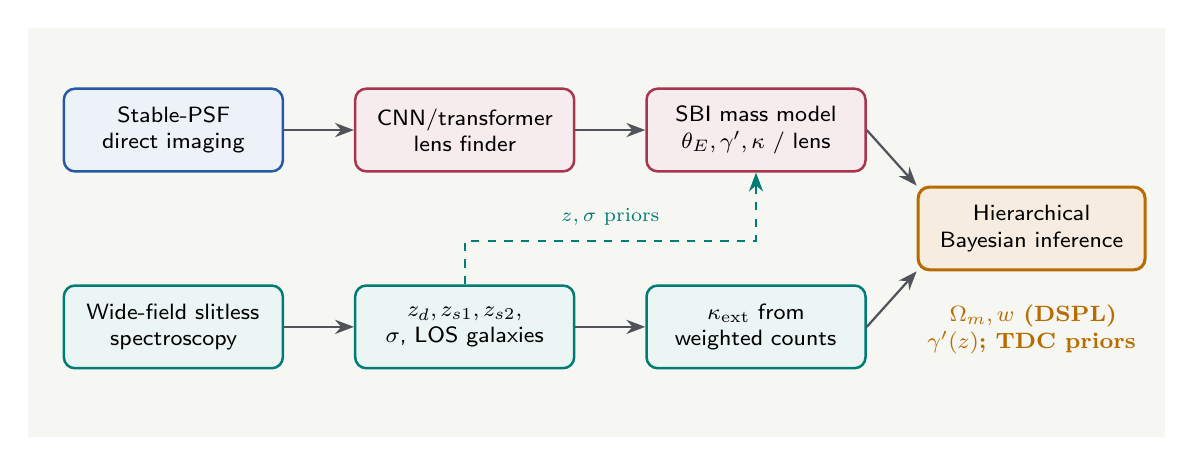
\begin{tikzpicture}[font=\sffamily\footnotesize,
  img/.style={rounded corners,draw=blue,line width=0.9pt,fill=blue!8,inner sep=4pt,align=center,text width=2.5cm,minimum height=1.05cm},
  spec/.style={rounded corners,draw=teal,line width=0.9pt,fill=teal!8,inner sep=4pt,align=center,text width=2.5cm,minimum height=1.05cm},
  ai/.style={rounded corners,draw=rose,line width=0.9pt,fill=rose!10,inner sep=4pt,align=center,text width=2.5cm,minimum height=1.05cm},
  outbox/.style={rounded corners,draw=gold,line width=1.1pt,fill=gold!12,inner sep=4pt,align=center,text width=2.6cm,minimum height=1.05cm},
  ar/.style={-{Stealth[length=2.4mm]},line width=0.8pt,color=ink!75},
  arp/.style={-{Stealth[length=2.4mm]},line width=0.8pt,color=teal,dashed}]
  \fill[paper] (-1.85,-2.65) rectangle (12.6,2.55);
  % columns at x = 0, 3.7, 7.4, 10.9 ; rows at y = +1.25 / -1.25
  \node[img]  (im)   at (0,1.25)    {Stable-PSF\\direct imaging};
  \node[spec] (sp)   at (0,-1.25)   {Wide-field slitless\\spectroscopy};
  \node[ai]   (find) at (3.7,1.25)  {CNN/transformer\\lens finder};
  \node[spec] (zz)   at (3.7,-1.25) {$z_d,z_{s1},z_{s2},$\\$\sigma$, LOS galaxies};
  \node[ai]   (sbi)  at (7.4,1.25)  {SBI mass model\\$\theta_E,\gamma',\kappa$ / lens};
  \node[spec] (kext) at (7.4,-1.25) {$\kappa_{\rm ext}$ from\\weighted counts};
  \node[outbox] (hier) at (10.9,0.0) {Hierarchical\\Bayesian inference};
  \node[anchor=north,text=gold,text width=3.0cm,align=center,font=\bfseries\footnotesize] at (10.9,-0.85)
       {$\Omega_m,w$ (DSPL)\\$\gamma'(z)$;\ TDC priors};
  % straight in-row arrows
  \draw[ar] (im)   -- (find);
  \draw[ar] (find) -- (sbi);
  \draw[ar] (sp)   -- (zz);
  \draw[ar] (zz)   -- (kext);
  % convergence to hierarchical layer
  \draw[ar] (sbi.east)  -- (hier.north west);
  \draw[ar] (kext.east) -- (hier.south west);
  % spectroscopy informs the mass model (dashed prior), routed clear of other arrows
  \draw[arp] (zz.north) -- ++(0,0.55) -| (sbi.south);
  \node[text=teal,font=\scriptsize,fill=paper,inner sep=1pt] at (5.55,0.15) {$z,\sigma$ priors};
\end{tikzpicture}
\caption{Strong-lensing analysis pipeline. Imaging (blue) drives machine-learning lens finding and simulation-based per-lens mass modeling. Spectroscopy (teal) supplies redshifts, dispersions, and line-of-sight galaxy counts for $\kappa_{\rm ext}$. A hierarchical Bayesian stage (gold) jointly infers cosmology and the population-level nuisance distributions, marginalizing each lens. Spectroscopy informs but does not gate the imaging-based core.}
\label{fig:lenspipe}
\end{figure}

\subsubsection{Weak-Lensing Cross-Checks and Program Scope}

Cosmic-shear weak lensing is not a primary product of this mission, because competitive shear requires the very large imaging areas of Rubin, \textit{Euclid}, and \textit{Roman}. The stable space-based PSF nonetheless makes \emph{targeted} weak lensing a useful internal cross-check rather than something to be excluded. Stacked galaxy--galaxy and group/cluster weak-lensing shear around the strong-lens deflectors constrains the mass at radii beyond the Einstein ring, providing an external handle on the mass-sheet that is independent of the stellar dynamics. For cluster-scale deflectors a joint strong$+$weak reconstruction tightens the total mass profile directly. These measurements use the same imaging already taken for lens finding and therefore add scientific value at no extra observational cost.

In scope, the strong-lensing program is a Years~2--5 effort that rides on the flagship survey's imaging and on fields shared with external time-delay campaigns, supplemented by targeted spectroscopy ($3\times2$--$3\times4$ hr in three roll angles) of the highest-value deflectors and all DSPL candidates. The deliverables are a spectroscopically confirmed lens and DSPL catalog with machine-learning mass models, a population measurement of $\gamma'(z,M_\ast)$, $\kappa_{\rm ext}$ and redshift support for external time-delay $H_0$ work, and a DSPL-based constraint on $(\Omega_m,w)$ that is independent of the mission's BAO and supernova results. This is a substantive, systematics-aware cosmology program built on the mission's real strengths, namely stable imaging, wide-field multiplexed spectroscopy, and automated inference, rather than a single-object $H_0$ claim.

\subsection{Lyman-\texorpdfstring{$\alpha$}{alpha} Forest, Absorption Systems, and Reionization}\label{sec:lyaforest}

The Lyman-$\alpha$ forest is the dense set of H\,\textsc{i} absorption lines imprinted on the spectrum of a background source by neutral hydrogen in the intergalactic medium (IGM) along the line of sight. Each absorber records the density, temperature, and peculiar velocity of diffuse gas at the redshift where Ly$\alpha$ ($\lambda_0=1215.67$\,\AA) comes into resonance. The forest is therefore a continuous tracer of large-scale structure across $2\lesssim z\lesssim4$, where few other tracers exist, and it underpins several distinct cosmological measurements. At higher column density the same absorbers steepen into Lyman-limit systems and damped Ly$\alpha$ absorbers, discrete tracers of circumgalactic and interstellar gas which this section surveys alongside the diffuse forest. We first set out what the forest delivers in principle, then quantify what the proposed $R=1000$ slitless spectrograph can measure, and define a program matched to that capability.

\subsubsection{The Forest as a Cosmological Probe}

Four measurements give the forest its cosmological weight. The first is the one-dimensional transmitted-flux power spectrum $P_{\rm 1D}(k)$, which probes the linear matter power spectrum on the smallest scales accessible to large-scale structure and is therefore sensitive to the summed neutrino mass and to the free-streaming of warm dark matter. The eBOSS measurement used about 44{,}000 quasars at $z>2.1$ \cite{chabanier2019}. The DESI DR1 analyses now reach beyond 300{,}000 Ly$\alpha$ quasars \cite{karacayli2025,ravoux2025}. Forest data set the strongest astrophysical lower bounds on the warm-dark-matter particle mass with $m_{\rm WDM}\gtrsim3.3$--$5.3$\,keV for an early-decoupled thermal relic \cite{viel2013,irsic2017}.

The second measurement is the thermal history of the IGM, encoded in the temperature-density relation. Power-spectrum and line-width analyses trace the gas temperature $T_0$ rising to $\sim1.4\times10^4$\,K near $z\approx3$ as He\,\textsc{ii} reionizes, and then cooling toward lower redshift \cite{walther2019,gaikwad2021}. The third is the baryon acoustic oscillation scale at $z\simeq2.3$, obtained from the three-dimensional correlation of Ly$\alpha$ absorption across many sightlines. This is the only BAO measurement deep in the matter-dominated era. eBOSS measured it from more than 210{,}000 quasars \cite{dumasdesbourboux2020}. DESI now reaches about 2\% precision from over 420{,}000 Ly$\alpha$ spectra \cite{desi2024lya}. The fourth is Ly$\alpha$ forest tomography. When sightlines are dense enough, the forest can be inverted into a three-dimensional map of IGM density that resolves cosmic-web filaments, voids, and protoclusters at $z>2$ \cite{lee2018clamato,newman2020latis}.

\subsubsection{Spectral Resolution and Detectable H\,I Columns}\label{sec:lyaresolution}

The interpretation of the forest depends critically on spectral resolution. A slitless mission has clear limits here. Individual forest absorbers have Doppler parameters of order $b\simeq20$--$30$\,km\,s$^{-1}$, set by the IGM temperature and turbulence \cite{rudie2012,rudie2013}. Resolving such a line requires a velocity resolution well below its width, in practice $R\gtrsim30{,}000$--$40{,}000$ as delivered by echelle spectrographs. The proposed instrument has $R=1000$, a resolution element of $c/R=300$\,km\,s$^{-1}$, roughly ten times broader than a single absorber. At the line density of the $z\simeq2.5$ forest every resolution element contains many blended lines. Hence, the spectrograph cannot decompose the forest into individual Voigt components.

What it can do is detect absorption above a flux-decrement threshold. We quantify this with the Ly$\alpha$ curve of growth, computed by integrating a Voigt profile to obtain the rest-frame equivalent width $W_\lambda$ as a function of the H\,\textsc{i} column density $N_{\rm H\,I}$ (Figure~\ref{fig:lyathreshold}, left). For an unresolved line, the minimum equivalent width detectable at significance $N_\sigma$ in a spectrum of resolution $R$ and continuum signal-to-noise ${\rm S/N}$ per resolution element is
\begin{equation}
W_{\min}^{\rm rest} \;=\; \frac{N_\sigma\,\lambda_0}{R\,({\rm S/N})},
\label{eq:wmin}
\end{equation}
where the $(1+z)$ factor of the observed-frame width and the rest-frame conversion cancel and, therefore, the threshold is independent of redshift. At $R=1000$ and a $5\sigma$ threshold, Eq.~\eqref{eq:wmin} gives $W_{\min}^{\rm rest}=0.61$\,\AA\ at ${\rm S/N}=10$ and $0.20$\,\AA\ at ${\rm S/N}=30$.

Inverting the curve of growth at these thresholds gives the minimum detectable column density (Figure~\ref{fig:lyathreshold}, right; Table~\ref{tab:lyathresh}). At ${\rm S/N}=10$ the mission detects only $N_{\rm H\,I}\gtrsim10^{16}$\,cm$^{-2}$. Reaching the diffuse forest near $N_{\rm H\,I}\sim10^{14}$\,cm$^{-2}$ requires ${\rm S/N}\gtrsim30$. The column densities between $\sim10^{14.5}$ and $\sim10^{19}$\,cm$^{-2}$ sit on the flat, saturated part of the curve of growth, where the equivalent width grows only logarithmically with $N_{\rm H\,I}$ and is degenerate with $b$. In this regime an $R=1000$ spectrum detects the absorption but cannot recover the column density from the Ly$\alpha$ line alone. As with the other slitless-calculator forecasts in this document (Section~\ref{sec:etc}), these thresholds are an idealised continuum-S/N calculation and carry the same optimistic margin relative to a fielded extraction pipeline.

\begin{figure}[tp]
\centering
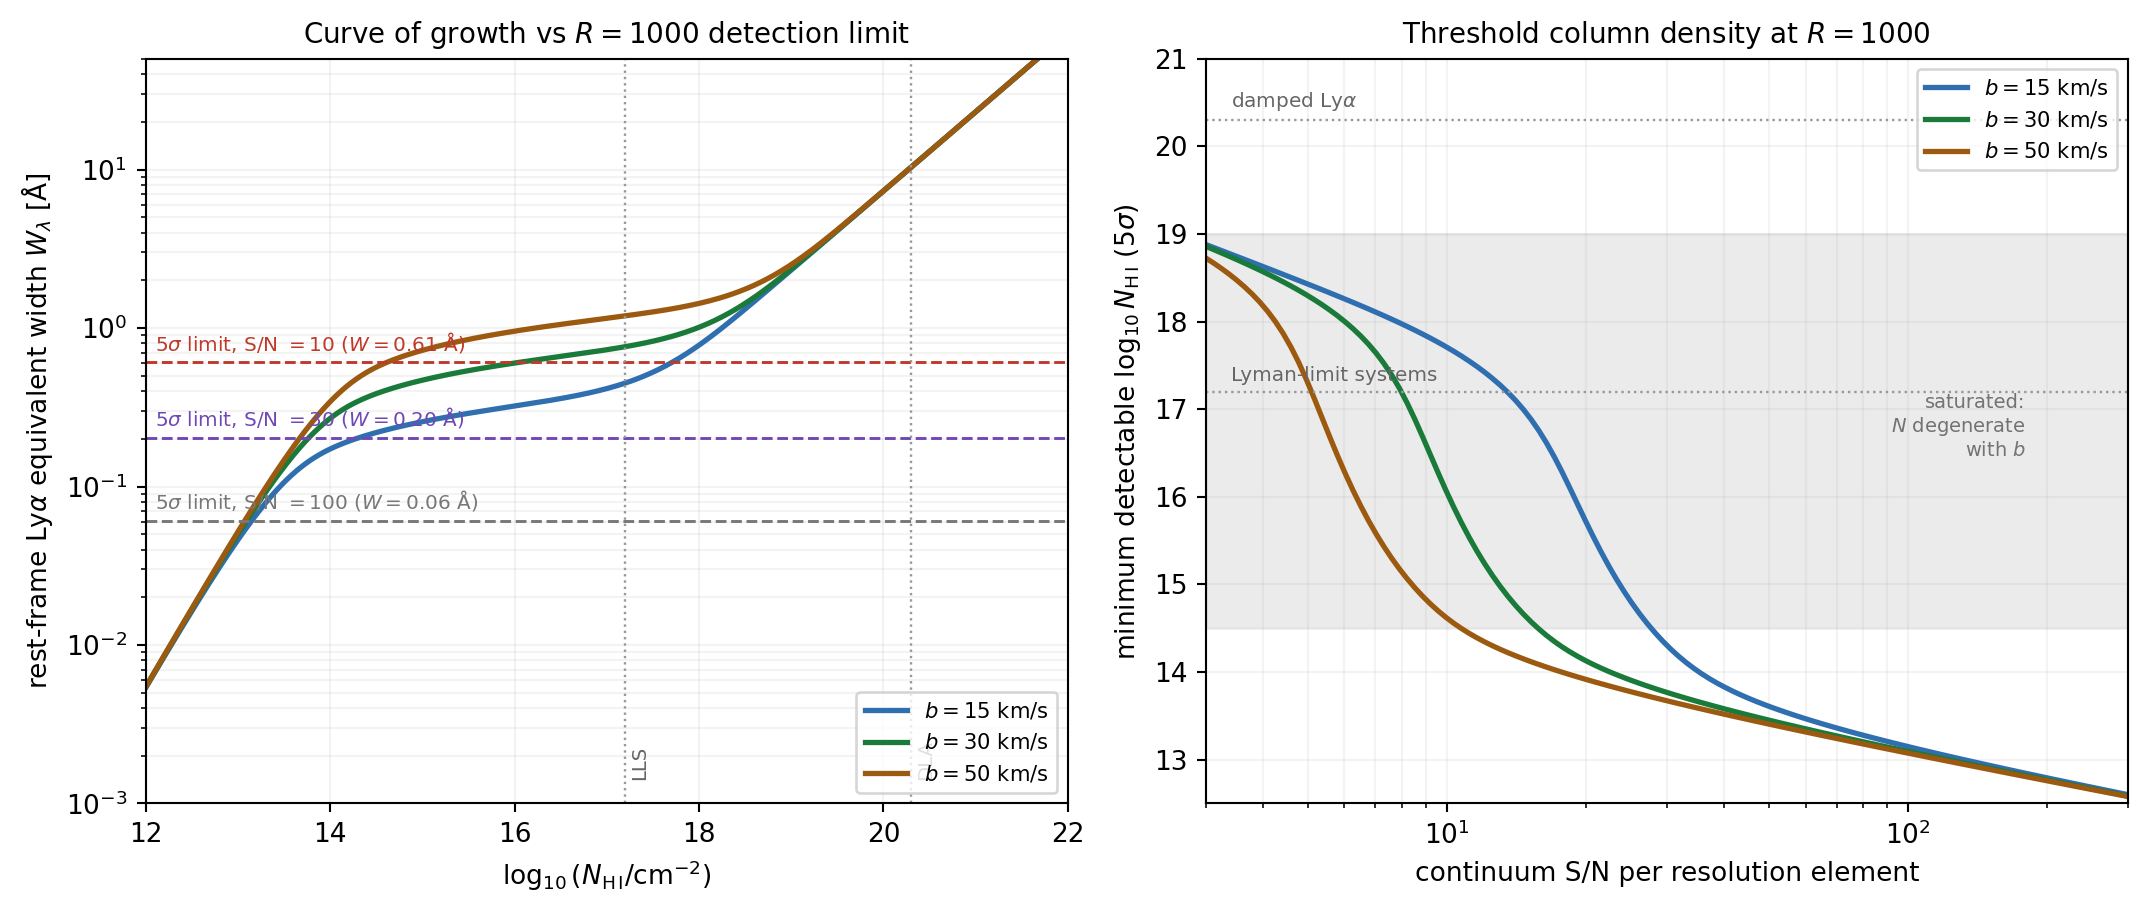
\includegraphics[width=0.85\textwidth]{lya_NHI_threshold.png}
\caption{What H\,\textsc{i} column density the $R=1000$ spectrograph can detect in the Ly$\alpha$ forest. \emph{Left}: the Ly$\alpha$ curve of growth, equivalent width $W_\lambda$ vs $\log N_{\rm H\,I}$, from a Voigt profile for Doppler parameters $b=15,30,50$\,km\,s$^{-1}$, with dashed $5\sigma$ detection limits of Eq.~\eqref{eq:wmin} for several continuum S/N values. The flat, saturated plateau between the linear and damping branches is where the column density cannot be inferred from the line. \emph{Right}: the resulting minimum detectable $\log N_{\rm H\,I}$ vs continuum S/N, with the saturated, $b$-degenerate regime shaded. Damped Ly$\alpha$ systems ($N_{\rm H\,I}\geq2\times10^{20}$\,cm$^{-2}$) lie on the damping branch and are measured accurately at $R=1000$.}
\label{fig:lyathreshold}
\end{figure}

\begin{table}[tp]
\centering
\sffamily\small
\begin{tabular}{@{}ccccc@{}}
\toprule
\textbf{Continuum S/N} & \textbf{$W_{\min}^{\rm rest}$} & \multicolumn{3}{c}{\textbf{minimum detectable $\log_{10}(N_{\rm H\,I}/{\rm cm^{-2}})$}}\\
(per res.\ element) & (\AA) & $b=15$ & $b=30$ & $b=50$ \\
\midrule
5 & 1.22 & 18.4 & 18.3 & 17.3\\
10 & 0.61 & 17.7 & 16.1 & 14.6\\
30 & 0.20 & 14.3 & 13.8 & 13.7\\
100 & 0.06 & 13.2 & 13.1 & 13.1\\
\bottomrule
\end{tabular}
\caption{Minimum detectable H\,\textsc{i} column density at $R=1000$ ($5\sigma$, Eq.~\eqref{eq:wmin}) for three Doppler parameters $b$ (km\,s$^{-1}$). Values with $\log N_{\rm H\,I}\gtrsim14.5$ fall on the saturated plateau of the curve of growth, where the column density is degenerate with $b$ and is not recoverable from the Ly$\alpha$ line alone.}
\label{tab:lyathresh}
\end{table}

Two regimes therefore remain robust at $R=1000$. The diffuse forest is measured statistically through the mean transmitted flux and the large-scale power spectrum rather than line by line. Damped Ly$\alpha$ absorbers, with $N_{\rm H\,I}\geq2\times10^{20}$\,cm$^{-2}$, develop damping wings tens of \AA\ wide in the observed frame, which are fully resolved at $R=1000$ and yield accurate column densities. The mission is thus a statistical-forest and damped-absorber instrument, not an echelle line-fitter.

\subsubsection{Tomographic Mapping with the Wide Survey}

The statistical forest matches the requirements of tomographic mapping, which needs many adjacent sightlines at moderate signal-to-noise rather than high resolution on a few. The achievable map resolution is set by the transverse sightline separation, which in turn depends on the surface density of usable background sources. At $z\simeq2.3$ the density of background galaxies and quasars usable as Ly$\alpha$ backlights rises steeply with depth from $\sim$360 to $\sim$3300\,deg$^{-2}$ between $g=24.0$ and $g=25.0$, giving mean transverse separations of $\sim3.6$ down to $\sim1.2\,h^{-1}$\,Mpc \cite{lee2014tomo}. CLAMATO realized this at $2.05<z<2.55$ with 240 sources over 0.157\,deg$^2$, a mean separation of $2.37\,h^{-1}$\,Mpc, and a map resolution of $2.5\,h^{-1}$\,Mpc (Figure~\ref{fig:lya3dexternal}) \cite{lee2018clamato}. LATIS extended this to 1.7\,deg$^2$ with about 3800 galaxy spectra at comparable resolution \cite{newman2020latis}.

\begin{figure}[tp]
\centering
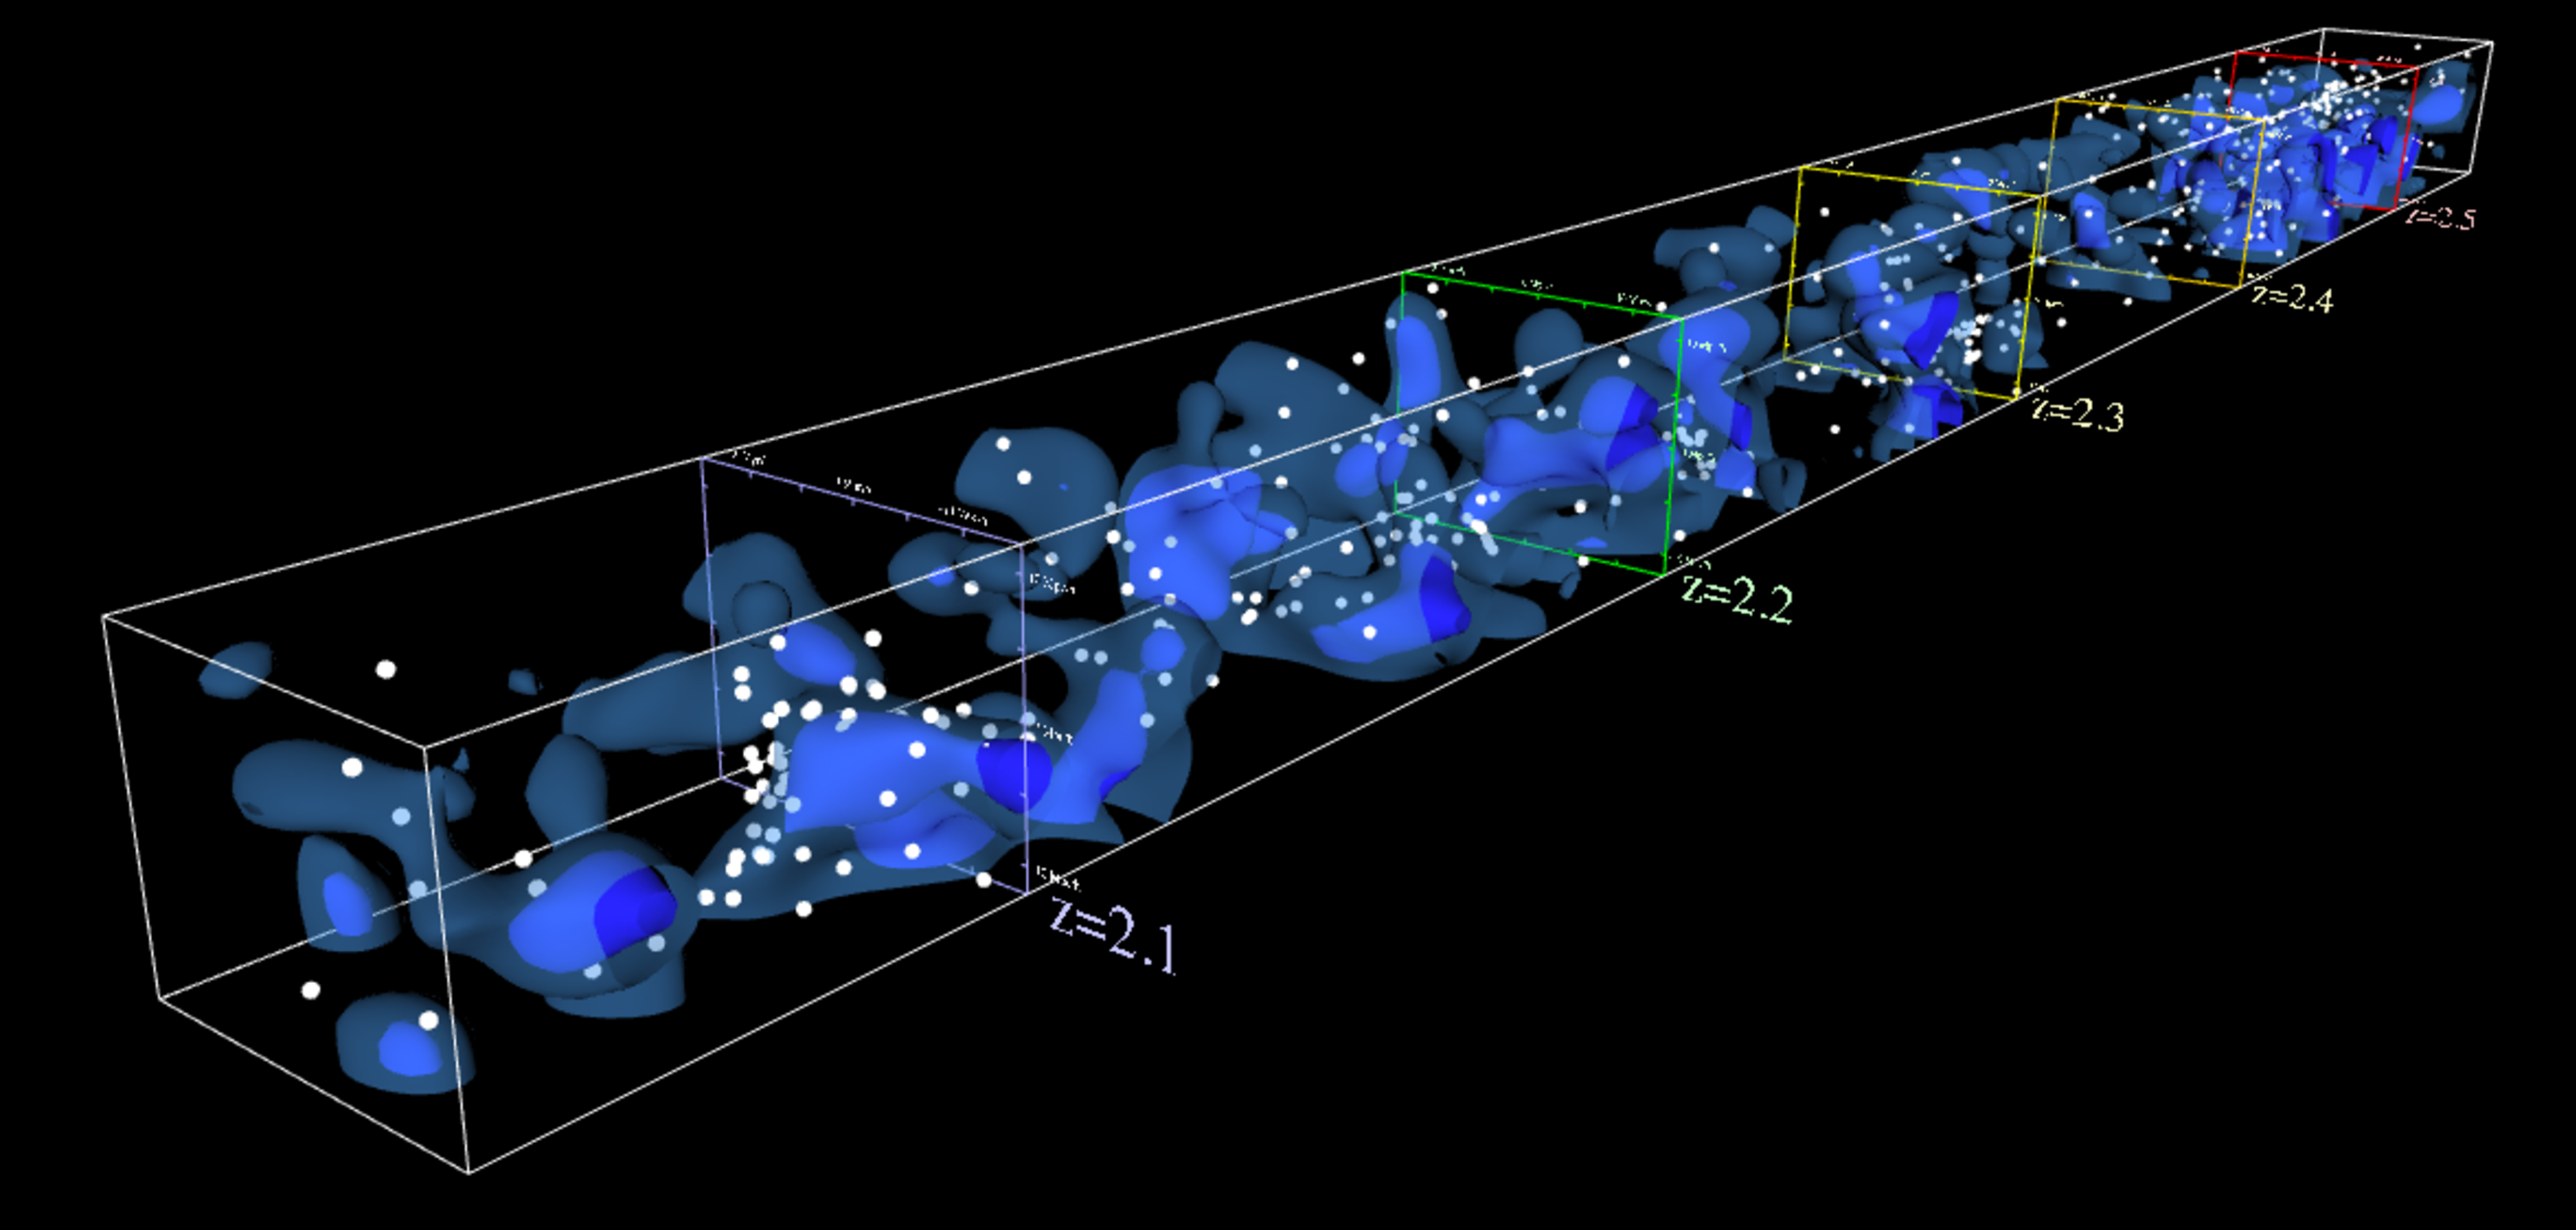
\includegraphics[width=0.85\textwidth]{lya_clamato_3d_external.png}
\caption{External 3D Ly$\alpha$ forest tomography visualization from the CLAMATO DR1 map. The blue isodensity surfaces show reconstructed IGM absorption structures while points mark coeval galaxies. This illustrates how multiple Ly$\alpha$ forest sightlines can be combined into a three-dimensional gas-density map. Image source: Lee et al. 2018, CLAMATO DR1, arXiv source figure \texttt{x3d\_screenshot\_v0.pdf} \cite{lee2018clamato}.}
\label{fig:lya3dexternal}
\end{figure}

For this mission, the wide multi-roll survey naturally collects faint star-forming galaxy and quasar continua across large contiguous areas, which is exactly the input tomography requires. A program targeting selected fields of about 1\,deg$^2$ to a few in signal-to-noise per resolution element on $g\lesssim24.5$ backlights would reach a transverse sampling near $2\,h^{-1}$\,Mpc, comparable to CLAMATO and LATIS but over a larger area. Such maps trace protoclusters and the cosmic web at $2\lesssim z\lesssim3$ and provide the density environment for the mission's own galaxy and quasar samples.

\subsubsection{Damped Ly$\alpha$ and Lyman-Limit System Census}

Damped Ly$\alpha$ absorbers (DLAs, $N_{\rm H\,I}\geq2\times10^{20}$\,cm$^{-2}$) and Lyman-limit systems (LLS, $N_{\rm H\,I}\gtrsim1.6\times10^{17}$\,cm$^{-2}$) trace the neutral-gas reservoir that fuels star formation. As shown in Section~\ref{sec:lyaresolution}, DLA damping wings are wide enough to be measured accurately at $R=1000$. Hence, a slitless quasar survey is an efficient DLA machine. Ground-based surveys have built large catalogs with more than 12{,}000 DLAs from SDSS-III \cite{noterdaeme2012}. Convolutional-network finders now identify and characterize DLAs in quasar spectra with about 97\% reliability for $\log N_{\rm H\,I}>19.5$, scaling to tens of thousands of systems \cite{parks2018}. The same machine-learning approach applies directly to the mission's homogeneous space-based spectra, which are free of telluric and sky-subtraction residuals. Anchored at $\langle z\rangle\simeq2.4$ by high-resolution work \cite{rudie2013}, the column-density distribution function and its evolution can be extended over the survey's large area to refine the neutral-gas mass density. The associated metal lines trace the chemical enrichment of the absorbers.

\subsubsection{Redshift Reach for Reionization}

Beyond the forest and its discrete absorbers, the same $0.36$--$3.0\,\mu$m band and quasar sightlines reach the epoch of reionization, the last global phase transition of the Universe, when ultraviolet photons from the first galaxies and quasars ionized the neutral hydrogen of the IGM. The cosmic microwave background fixes its integrated effect through the Thomson optical depth $\tau=0.0544\pm0.0073$, which corresponds to a midpoint near $z_{\rm re}=7.67\pm0.73$ \cite{planck2018}, but the detailed history, how the volume-averaged neutral fraction $\bar{x}_{\rm H\,I}$ evolved and how patchy the process was, is still being mapped. Unlike the forest, the reionization observables are broad spectral features, well matched to this mission's resolution rather than limited by it. Redshifted Ly$\alpha$ enters the blue edge of the band at $z\simeq2.0$ and remains in band up to $z=(30000/1215.67)-1\simeq23.7$, and the Lyman break at $912$\,\AA\ stays in band from $z\simeq2.9$ to $z\simeq32$, so the mission can observe the Ly$\alpha$ damping wing, Ly$\alpha$ emission, and the rest-frame ultraviolet continuum across the entire reionization era and beyond, into the redshift range the first JWST spectra are now opening up. The broad features that diagnose reionization, namely damping wings, Gunn-Peterson troughs, and proximity zones, span tens to hundreds of \AA\ in the observed frame, which the $300$\,km\,s$^{-1}$ resolution element resolves comfortably.

\subsubsection{Quasar Damping Wings and the Neutral Fraction}

The cleanest single-object probe of $\bar{x}_{\rm H\,I}$ is the IGM damping wing redward of Ly$\alpha$ in a luminous $z>7$ quasar. A neutral IGM produces a smooth absorption wing whose shape and depth scale with the neutral fraction. The feature is broad enough that $R=1000$ measures it accurately. Since the discovery of ULAS\,J1120+0641 at $z=7.085$ \cite{mortlock2011}, damping-wing modeling of the growing $z>7$ quasar sample has returned neutral fractions that rise steeply through the EoR. Two quasars at $z=7.09$ and $z=7.54$ give $\bar{x}_{\rm H\,I}\approx0.48$ and $\approx0.60$ \cite{davies2018}, J0252$-$0503 at $z=7.0$ gives $\approx0.70$ \cite{wang2020}, and independent analyses of J1120 and J1342 span $\bar{x}_{\rm H\,I}\approx0.4$ at $z\approx7.1$ to $\approx0.2$--$0.4$ at $z\approx7.5$ \cite{greig2017,greig2019}, with a third quasar at $z\approx7.5$ giving a consistent value \cite{yang2020}. The spread across objects is itself informative, since it reflects the patchiness of reionization.

The end of the process is pinned by the Gunn-Peterson trough in $z\simeq6$ quasars, where the Ly$\alpha$ optical depth steepens sharply and the transmitted flux vanishes \cite{fan2006}. Long dark troughs persisting below $z\simeq6$ require large-scale fluctuations in the neutral fraction \cite{becker2015}. The XQR-30 sample shows that a uniform ionizing background is excluded until $z\approx5.3$. Therefore, reionization ends later than once assumed \cite{bosman2022}. Model-independent dark-pixel counts bound the neutral fraction from above with $\bar{x}_{\rm H\,I}\lesssim0.06$ by $z\simeq5.9$ \cite{mcgreer2015}. Bright $z>6.5$ quasars from Euclid, Roman, and Rubin/LSST will supply the targets, although the subset bright enough for high-quality damping-wing work is modest \cite{mortlock2024}.

\subsubsection{Ly$\alpha$ Emission from Galaxies}

Galaxies provide a complementary and far more numerous probe through their Ly$\alpha$ emission, which is resonantly scattered by neutral hydrogen and therefore suppressed when the surrounding IGM is neutral. The fraction of Lyman-break galaxies showing strong Ly$\alpha$ emission rises toward $z\simeq6$, where roughly half of faint galaxies have rest-frame equivalent widths above $25$\,\AA\ \cite{stark2010,stark2011}, and then drops at $z\simeq7$ in a spatially patchy way \cite{pentericci2014}. Modeling this decline yields neutral fractions of $\bar{x}_{\rm H\,I}\approx0.59$ at $z\sim7$ \cite{mason2018}, $\approx0.49$ at $z\simeq7.6$ \cite{jung2020}, and as high as $\approx0.88$ at $z\simeq7.6$ in one analysis \cite{hoag2019}. The Ly$\alpha$ equivalent-width distribution and its evolution with redshift are the key observables. Both are directly measured from the mission's spectra.

JWST has now pushed Ly$\alpha$ studies into the heart of the EoR. GN-z11 shows Ly$\alpha$ emission at $z=10.6$ \cite{bunker2023}, four galaxies have been confirmed at $z=10.3$--$13.2$ with Lyman-edge damping wings consistent with a largely neutral IGM \cite{curtislake2023}. Ly$\alpha$ emission has been detected at $z\simeq13$, signaling an early ionized region around a luminous galaxy \cite{witstok2025}. These results define the science frontier that a wide-field, $0.36$--$3.0\,\mu$m slitless survey is built to populate statistically. Where JWST observes a handful of objects with a small field, this mission can assemble large, uniform samples of Ly$\alpha$ emitters and Lyman-break galaxies across many independent sightlines, which is what is required to map the patchiness of reionization rather than sample it.

\subsubsection{Synergy with 21\,cm and the CMB}

The Ly$\alpha$ observables are most powerful in combination with the redshifted 21\,cm line, which traces the neutral gas directly. HERA Phase I has begun to constrain the 21\,cm power spectrum and already requires that the IGM was heated above the adiabatic-cooling floor by $z\approx10.4$, ruling out the coldest reionization scenarios \cite{hera2023}. SKA will map the signal in tomography. Galaxy Ly$\alpha$ and quasar damping wings localize the ionized and neutral regions that the 21\,cm experiments measure in aggregate. Hence, cross-correlation between this mission and 21\,cm surveys breaks degeneracies that neither probe resolves alone. The CMB optical depth \cite{planck2018} provides the integral constraint that any reconstructed history must reproduce.

\subsubsection{Program Scope and Synergy}

The Ly$\alpha$ program is scoped as a calibration, tomography, and absorber-census effort rather than a competitor to DESI-scale BAO. DESI already measures the Ly$\alpha$ BAO and $P_{\rm 1D}$ from hundreds of thousands of sightlines \cite{desi2024lya,karacayli2025}, and the present mission does not aim to match that statistical power, especially since forest $P_{\rm 1D}$ does not by itself tighten the summed-neutrino-mass bound once combined with other probes \cite{chaves2026}. The adopted forest program is 3000--5000 quasars at $2.1<z<3.5$, selected to $m_{\rm AB}\lesssim21.5$ for 1--2\,hr spectra and extended to $m_{\rm AB}\simeq22.5$ in 4--6\,hr calibration fields over 1000--3000\,\degti\ of parent imaging. The reionization program is a separate, high-value, modest-volume effort riding the same quasar-targeting infrastructure. It adopts 50--100 quasars at $z>6.5$ with $3\times2$--$3\times5$\,hr spectra for damping-wing neutral-fraction measurements, plus 100--200 bright Ly$\alpha$ emitters and Lyman-break galaxies in known overdensities with $3\times5$--$3\times10$\,hr integrations for the Ly$\alpha$ fraction test. The continuum signal-to-noise and radiative-transfer interpretation are the limiting factors for the galaxy sample, so it is scoped as a deep, targeted program rather than a blind wide survey. The combined deliverables are a homogeneous space-based quasar reference sample cross-calibrated against DESI and high-resolution echelle data, selected megaparsec-resolution tomography fields, a large DLA and LLS catalog with metal-line measurements, a uniform set of damping-wing neutral-fraction measurements across $6.5\lesssim z\lesssim8$, a Ly$\alpha$ equivalent-width distribution as a function of redshift, and ionized-region maps for cross-correlation with 21\,cm experiments. High-resolution ground-based spectroscopy remains the source of individual $b$ and $N_{\rm H\,I}$ values on a subset. The mission's role throughout is to supply the wide, uniform, space-stable quasar-sightline coverage that ground surveys cannot.

\subsection{Low-Surface-Brightness Galaxies and the Dark Matter of Clusters}\label{sec:lsb}

The low-surface-brightness (LSB) Universe is the part of the galaxy population that lies below the night-sky background. It is precisely the part that ordinary flux-limited surveys miss. Diffuse stellar systems, the faint outer envelopes of galaxies, and the intracluster light which fills the space between cluster members all encode information that the bright, high-contrast Universe does not. For dark matter this matters directly. In a galaxy cluster the baryons that are easiest to see, the member galaxies and the X-ray gas, are dynamically subdominant and spatially biased relative to the total mass. The faint diffuse light, by contrast, turns out to follow the dark matter remarkably well. The program therefore runs in two complementary modes. The first is a blind imaging census. It costs no extra observing time because it rides the same wide, medium, and deep tiers as the flagship survey. It finds the field LSBGs and UDGs, characterising them together with the void dark-galaxy candidates of Section~\ref{sec:dwarfvoid}. The second is a targeted deep mode. It spends long multi-roll exposures on $\sim$20--40 nearby clusters to map the ultra-diffuse galaxies and the intracluster light as tracers of the cluster dark matter distribution.

These three target classes are not confirmed the same way. An LSBG is defined by its observed surface brightness, a quantity the imaging measures directly. Therefore, no distance is needed to place a candidate in the catalog. A UDG is defined instead by its physical effective radius, a size in kiloparsecs rather than in arcseconds. Converting the angular size the imaging measures into that physical size requires a distance. A UDG classification is therefore confirmed only once a redshift is in hand, from an emission line in the slitless spectrum for a gas-rich system or from the assumed cluster distance for a quiescent one in a known cluster. A void galaxy carries the same requirement for a different reason. Its membership is decided by its true three-dimensional position inside a cataloged void rather than by its position on the sky alone, since a flat sky projection also captures galaxies that merely lie in front of or behind the void along the line of sight (Section~\ref{sec:voidphenom}). Confirming that position again requires a redshift. What follows keeps this distinction in view, LSBG discovery from imaging alone against UDG and void confirmation from imaging paired with spectroscopy.

\subsubsection{The Low-Surface-Brightness Regime and Why It Demands Space}

Surface brightness, unlike flux, is preserved under distance in a static universe. Cosmological dimming degrades it strongly, $\mu(z)=\mu_0+10\log_{10}(1+z)$ mag\,arcsec$^{-2}$, the $(1+z)^4$ law. An ultra-diffuse galaxy with a central surface brightness of $\mu_0\simeq24$ mag\,arcsec$^{-2}$ is dimmed by $1.1$ mag by $z=0.3$ and by $3$ mag by $z=1$. It then sinks far below the few-percent level of sky-background control that ground-based imaging can realistically achieve. The limiting factors on the ground are not photon statistics but systematics. The airglow is bright and variable. Scattered light and flat-fielding errors add structure on exactly the large angular scales that diffuse sources subtend. The faintest reliable ground-based surface-brightness limits reach $\mu\sim28$--$29$ mag\,arcsec$^{-2}$. The purpose-built Dragonfly Telephoto Array, designed specifically to suppress scattered light, pushes to $\mu\sim30$--$31$ mag\,arcsec$^{-2}$ \cite{abraham2014dragonfly}. A space platform removes the airglow term entirely. It also stabilizes the point-spread function and the photometric response. The achievable depth is then set by integration time and by the Galactic cirrus foreground rather than by a fluctuating sky. Long exposures over a wide, contiguous field are therefore the natural mode in which a space telescope outperforms larger ground-based apertures for diffuse science. That combination is precisely what the mission's \fovlarge\ field delivers. Figure~\ref{fig:lsbggallery} shows what this population actually looks like. Its twelve galaxies from the published DES low-surface-brightness catalog \cite{tanoglidis2021} span mean surface brightness $\bar\mu_g=25.0$--$27.2$ mag\,arcsec$^{-2}$. The faint end is already at the edge of visibility in some of the deepest wide-area ground imaging in existence.

\begin{figure}[tp]
\centering
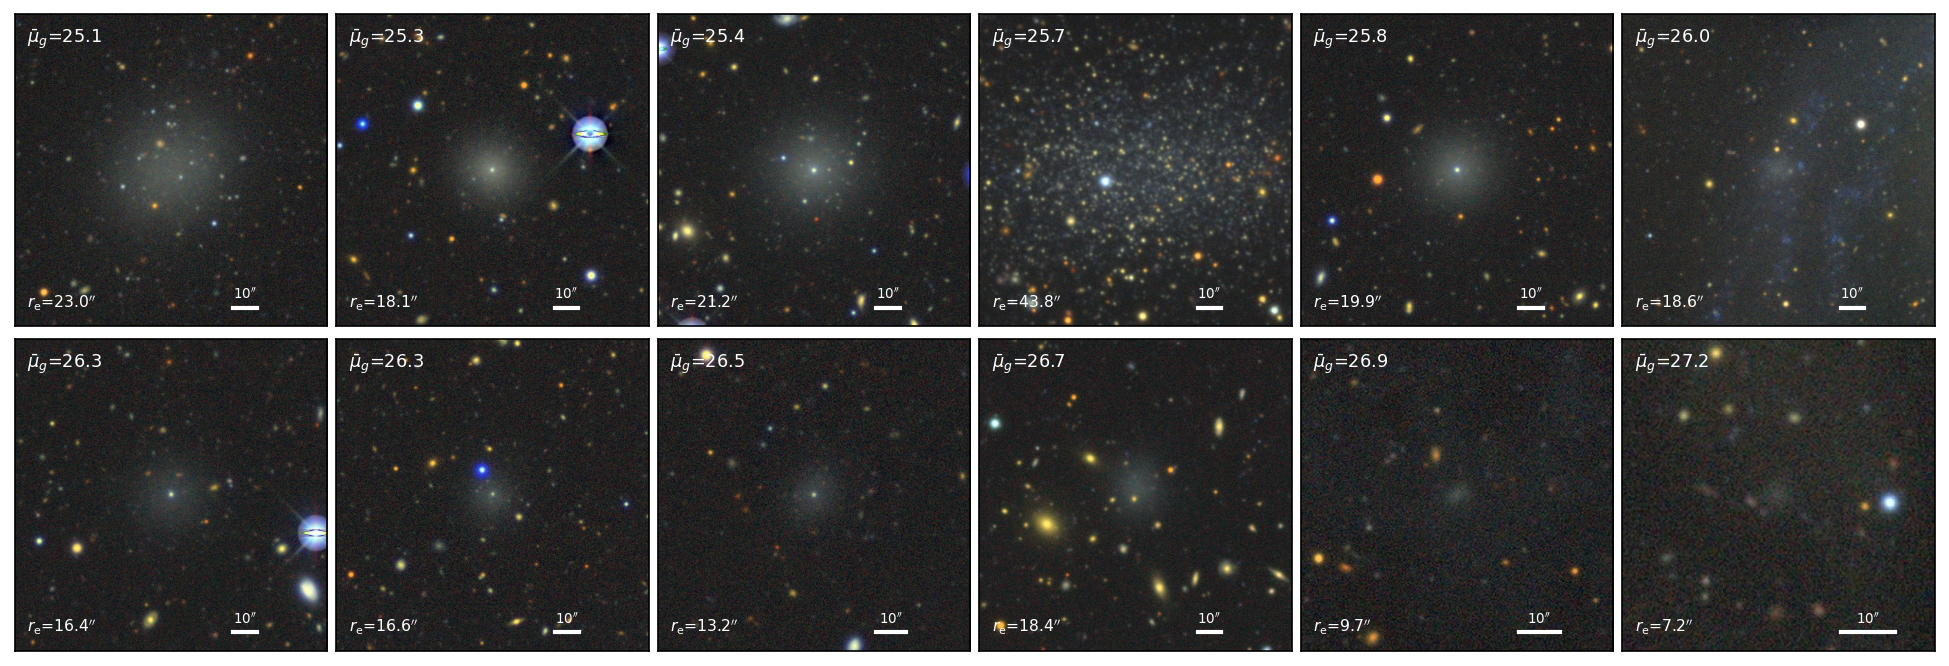
\includegraphics[width=\textwidth]{des_lsbg_gallery.png}
\caption{Twelve low-surface-brightness galaxies from the published DES DR1 LSBG catalog of 23{,}790 objects \cite{tanoglidis2021}, in DECam Legacy Surveys DR10 colour imaging \cite{dey2019}. Panels are ordered by mean $g$-band surface brightness across twelve equal bins spanning $\bar\mu_g=25.0$--$27.2$ mag\,arcsec$^{-2}$, the range the published catalog populates, each showing the angularly largest object with its $\bar\mu_g$, effective radius, and a $10''$ scale bar. The brightest examples are obvious, the $\bar\mu_g\simeq26$ objects are already marginal, and the faintest nearly vanish in imaging that represents the state of the art for wide ground-based surveys. The parameter space beyond $\bar\mu_g\simeq27$, where the fuzzy-dark-matter candidate Nube lies (Figure~\ref{fig:nube}), is essentially unexplored over wide areas, exactly the regime the mission's $\mu\sim30$--$32$ mag\,arcsec$^{-2}$ reach opens.}
\label{fig:lsbggallery}
\end{figure}

\subsubsection{Ultra-Diffuse Galaxies as a Cluster Population}

The clearest recent demonstration of the hidden LSB population is the discovery of ultra-diffuse galaxies (UDGs). Deep imaging of the Coma cluster with Dragonfly revealed 47 Milky-Way-sized but extremely diffuse galaxies, objects with effective radii $r_{\rm e}\gtrsim1.5$\,kpc yet central surface brightness $\mu_0(g)\gtrsim24$ mag\,arcsec$^{-2}$ and stellar masses one hundred to one thousand times below the Milky Way \cite{vandokkum2015coma}. Follow-up with the wider field of Subaru/Suprime-Cam expanded the Coma census to roughly a thousand such systems \cite{koda2015,yagi2016}. Comparable populations were found in Virgo and other clusters \cite{mihos2015}. That these fragile, low-density systems survive in the cluster tidal field at all implies that many sit inside massive dark matter halos. Beyond clusters, the SMUDGes program has extended the census to the field, selecting $7{,}070$ UDG candidates over the full DECam Legacy Surveys footprint \cite{zaritsky2023}. Figure~\ref{fig:udggallery} shows twelve of its candidates over the DES southern sky, spanning central surface brightness $\mu_{0,g}=24.0$--$27.7$ mag\,arcsec$^{-2}$.

\begin{figure}[tp]
\centering
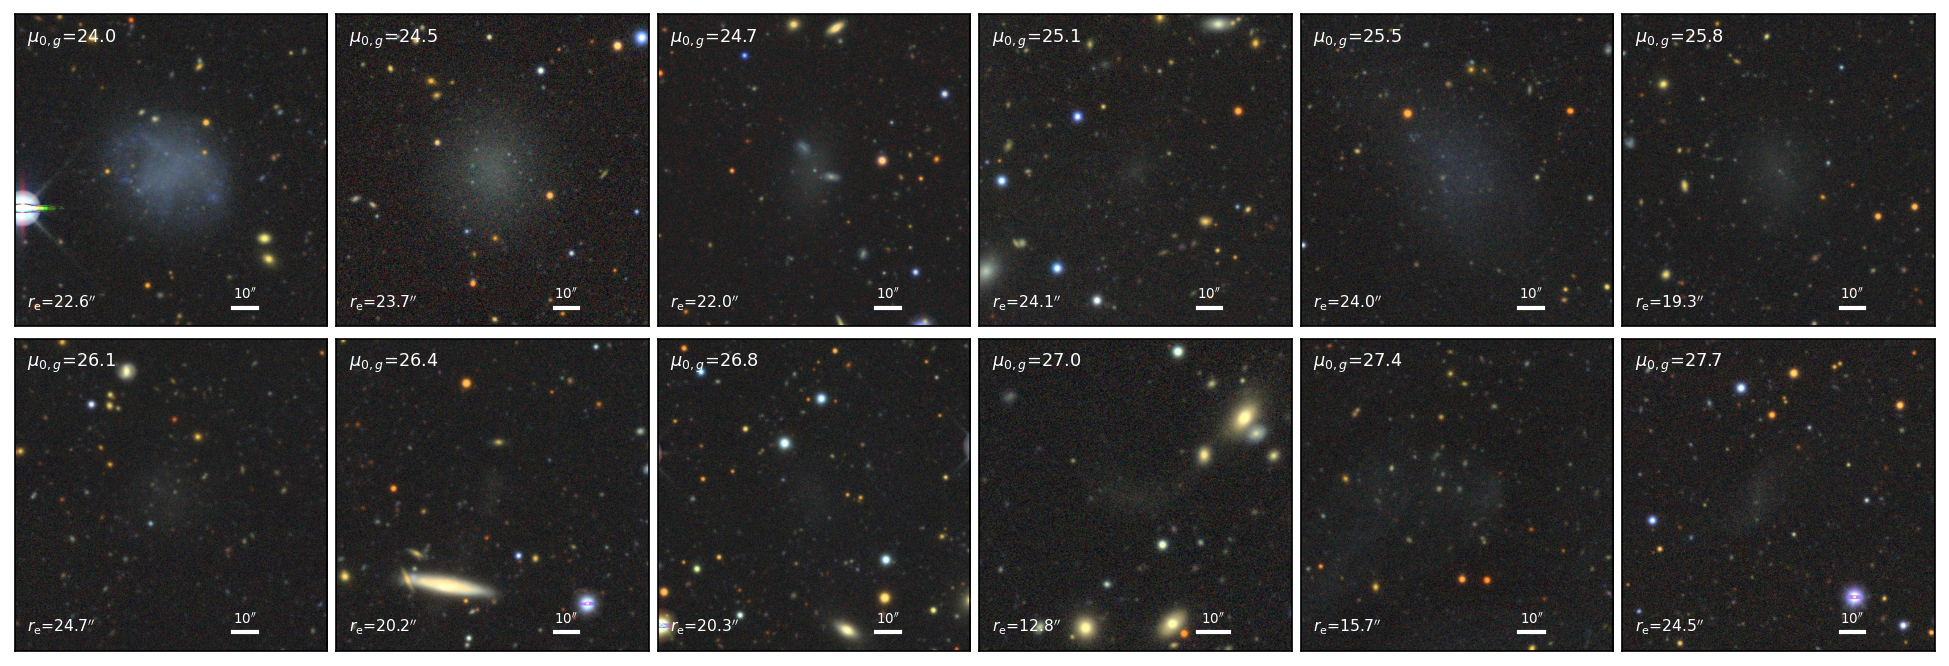
\includegraphics[width=\textwidth]{des_udg_gallery.png}
\caption{Twelve ultra-diffuse-galaxy candidates over the DES southern sky (Dec $<+5^\circ$) from the published SMUDGes catalog of $7{,}070$ candidates selected over the DECam Legacy Surveys footprint with $r_{\rm e}\geq5.3''$ and $\mu_{0,g}\geq24$ mag\,arcsec$^{-2}$ \cite{zaritsky2023}, shown in Legacy Surveys DR10 colour imaging \cite{dey2019}. The panels are ordered across twelve equal bins of central surface brightness spanning $\mu_{0,g}=24.0$--$27.7$ mag\,arcsec$^{-2}$, showing the angularly largest candidate per bin among those with $r_{\rm e}\leq25''$, with a $10''$ scale bar. As in Figure~\ref{fig:lsbggallery} the faint end of the published population sits at the edge of visibility in the deepest wide-area ground imaging. The UDG census, its cluster-to-field comparison, and the dark-matter statistics built on them (Section~\ref{sec:lsb}) therefore require the space-based surface-brightness reach of this mission.}
\label{fig:udggallery}
\end{figure}

The dark matter content of UDGs is, however, strikingly bimodal. That bimodality is what makes them interesting for the nature of dark matter rather than merely for galaxy formation. At one extreme sits Dragonfly\,44 in Coma. Its stellar velocity dispersion of $\sigma\simeq47$ km\,s$^{-1}$ and its roughly one hundred globular clusters imply a dynamical mass within the half-light radius of order $10^{10}\,M_\odot$ and a dark-matter fraction near unity, comparable to that of a galaxy a hundred times more luminous \cite{vandokkum2016df44}. At the other extreme lie NGC\,1052--DF2 and NGC\,1052--DF4. The globular-cluster and stellar kinematics of these two UDGs give dispersions of only $\sigma\simeq3$--$4$ km\,s$^{-1}$, consistent with the baryonic mass alone and apparently \emph{lacking} dark matter \cite{vandokkum2018df2,vandokkum2019df4}. Dark-matter-free galaxies are not predicted by collisionless cold dark matter without an external stripping or collisional formation channel. Hence, confirming, counting, and locating such systems within their host environments is a direct test of structure formation. The internal stellar dispersions themselves, a few to a few tens of km\,s$^{-1}$, lie below the $300$ km\,s$^{-1}$ resolution element of an $R=1000$ spectrograph and remain the domain of high-resolution follow-up. What the mission supplies is the step that gates all of this work, a deep, wide, uniform photometric and slitless census. The census finds the systems. It establishes cluster membership through the redshift of any emission or strong absorption features and through the radial velocities of associated compact sources. It characterizes their structure and stellar populations across an entire cluster in a single pointing.

\subsubsection{A Field Census of LSBGs and UDGs from the Wide Survey}

The cluster program above is targeted, but the mission produces a second low-surface-brightness census at no additional observing cost, because the direct imaging taken for the flagship ELG survey already covers the $100$--$300$\,deg$^2$ wide footprint and its nested medium and deep tiers. Table~\ref{tab:lsbsurvey} gives the surface-brightness reach of that imaging from the exposure-time calculator. Even the wide tier goes roughly three magnitudes deeper than the DES imaging from which the published catalogs of Figures~\ref{fig:lsbggallery} and \ref{fig:udggallery} were selected. Therefore, the guaranteed floor is set by the published surface densities themselves. The DES DR1 catalog contains $23{,}790$ LSBGs over $\sim$5{,}000\,deg$^2$, about $4.8$ per deg$^2$ to its $\bar\mu_g\simeq27.2$ limit \cite{tanoglidis2021}. Hence, the wide footprint alone contains five hundred to fourteen hundred such galaxies. Beyond them the so far unexplored population at $\bar\mu_g\gtrsim27$, the regime of the almost-dark galaxy Nube (Figure~\ref{fig:nube}), is opened over hundreds of square degrees for the first time.

\begin{table}[tp]
\centering
\sffamily\small
\begin{tabularx}{\textwidth}{@{}p{2.2cm}p{2.2cm}p{2.6cm}p{2.6cm}X@{}}
\toprule
\textbf{Tier} & \textbf{Exposure} & \textbf{$\mu_{5\sigma}(10'')$, $g$} & \textbf{$\mu_{5\sigma}(10'')$, $H$} & \textbf{Role for the LSB census}\\
\midrule
Wide ($\sim$150\,deg$^2$/cap) & $0.75$ hr & $29.8$ & $29.5$ & Discovery over the full footprint, three magnitudes past the DES selection\\
Medium (30\,deg$^2$) & $3$ hr & $30.6$ & $30.3$ & Structural parameters and colour gradients for the faint tail\\
Deep (1--3\,deg$^2$) & $12$ hr & $31.3$ & $31.0$ & The $\bar\mu\gtrsim28$ regime, unexplored beyond individual objects\\
\bottomrule
\end{tabularx}
\caption{Surface-brightness reach of the flagship-survey direct imaging for the field LSBG and UDG census from the exposure-time calculator over a $10\times10$\,arcsec$^2$ bin. The census comes free with the wide survey. The published DES surface density of $4.8$ LSBGs per deg$^2$ \cite{tanoglidis2021} sets its guaranteed floor.}
\label{tab:lsbsurvey}
\end{table}

What turns this catalog into physics is the spectroscopy taken simultaneously. UDG classification requires the physical effective radius and therefore a distance. For the published field candidates that distance rests on assumed cluster association or on expensive one-by-one follow-up \cite{zaritsky2023}. The slitless survey enables us to obtain redshifts for every LSBG with emission lines directly, since gas-rich low-surface-brightness systems have exactly the high line-to-continuum contrast the selection favours (Section~\ref{sec:lsb} and the void program of Section~\ref{sec:dwarfvoid}). Each such redshift converts an angular size into a physical one. It confirms or rejects the UDG classification on the spot. The survey's own three-dimensional ELG density field supplies the environment of every candidate. The result is a UDG and LSBG census with uniform selection, physical sizes for the emission-line subset, and an environmental axis running from voids through the field to groups. That is precisely the population-level input the dark-matter tests of Section~\ref{sec:dwarfvoid} and Table~\ref{tab:dmmodels} require.

For the faintest diffuse work the program adds two dedicated ultra-deep imaging fields, deliberately far smaller than the blind census, which keeps riding the full survey tiers. Each field is a $3\times3$ block of $30'$ tiles, $1.5^\circ$ on a side and $2.25$\,deg$^2$, sited on the cleanest sky available, found by minimising the mean Planck 857\,GHz intensity over a $7^\circ$ aperture across all $|b|>48^\circ$ sky \cite{planck2018hfi}. The minima fall at $(\alpha,\delta)=(210^\circ,+38^\circ)$, $b=+72^\circ$, in the north, just outside the corner of the flagship Bo\"otes wide tier, and $(344^\circ,-48^\circ)$, $b=-59^\circ$, in the south. Their field-mean $857$\,GHz intensities are $0.97$ and $0.92$\,MJy\,sr$^{-1}$, about a quarter of the all-sky median of $3.6$\,MJy\,sr$^{-1}$ and $\sim30\%$ below the SXDS window ($1.30$\,MJy\,sr$^{-1}$). The top row of Figure~\ref{fig:imgfields} zooms on both fields, confirming directly on the dust map that the footprints are free of cirrus structure. Their locations are marked on the all-sky view of Figure~\ref{fig:skymap}. The fields are observed in the five survey bands, $g$ ($0.5\,\mu$m) and $z$ ($0.9\,\mu$m) on the CCD arm and $J$, $H$, and $K$ ($1.2$, $1.6$, $2.2\,\mu$m) on the HgCdTe arm (Figure~\ref{fig:compareimg}). Because the dichroic feeds both arms simultaneously, the deep $g$ and $H$ pair is collected at once. Sixteen hours per tile in that pair reach $\mu_{5\sigma}(10'')=31.5$ in $g$ and $31.2$ in $H$ from the exposure-time calculator, the regime of the almost-dark galaxy Nube (Figure~\ref{fig:nube}), for about $290$\,hr over both caps. Two shallower passes add $z$, $J$, and $K$ for the colours, stellar-population diagnostics, and photometric redshifts of the catalog.

In the opposite direction the imaging also extends far beyond the spectroscopic footprint, since imaging-only tiles are cheap. An imaging-only wide extension adds a $35\times35$-tile field, $17.5^\circ$ on a side and $\sim$306\,deg$^2$, per cap, sited by the same cirrus-minimisation criterion with a matching aperture. The northern extension field, at $(\alpha,\delta)=(162^\circ,+52^\circ)$, $b=+56^\circ$, sits beside the Lockman Hole, the classic low-column window of the northern sky. The southern field, at $(3^\circ,-38^\circ)$, $b=-77^\circ$, lies near the south Galactic pole. Both fields have footprint-mean $857$\,GHz intensities of $0.97$\,MJy\,sr$^{-1}$. A quarter of an hour per tile in the simultaneous $g$+$H$ pair reaches $\mu_{5\sigma}(10'')=29.2$ in $g$ and $28.9$ in $H$, still about two magnitudes past the DES imaging behind Figures~\ref{fig:lsbggallery} and \ref{fig:udggallery}, for about $610$\,hr in total. The extension roughly triples the area of the blind census, raising its guaranteed floor at the published DES surface density \cite{tanoglidis2021} to over three thousand LSBGs. Because the imaging-only wide extension and the two ultra-deep fields carry no spectroscopy, they extend the LSBG catalog alone. A candidate found there enters the confirmed UDG sample only once an external facility supplies its distance, and it plays no part in the void-membership test of Section~\ref{sec:voidphenom}, which needs that same redshift-based three-dimensional position. Both extension fields are marked in magenta on Figure~\ref{fig:skymap} and zoomed in the bottom row of Figure~\ref{fig:imgfields}. The flat-field and cirrus-foreground control that this diffuse photometry requires is common to every imaging program of the mission and is treated in Section~\ref{sec:flatcirrus}.

\begin{figure}[tp]
\centering

\includegraphics[width=\textwidth]{imaging_fields_zoom.png}
\caption{The four dedicated imaging fields on the Planck 857\,GHz thermal-dust map \cite{planck2018hfi}, same gnomonic (TAN) projection and graticule as Figure~\ref{fig:deepzoom}. \emph{Top row}: the two ultra-deep fields ($3\times3$ tiles, $2.25$\,deg$^2$ each), minima of the mean $857$\,GHz intensity over a $7^\circ$ aperture across all $|b|>48^\circ$ sky. \emph{Bottom row}: the two imaging-only wide-extension fields ($35\times35$ tiles, $\sim$306\,deg$^2$ each), minima with a matching aperture over $|b|>55^\circ$, beside the Lockman Hole in the north and the south Galactic pole in the south. Each footprint is annotated with its measured mean intensity, about a quarter of the all-sky median in all four panels. The SN Ia time-domain cadence fields sit inside the wide tier instead and appear in Figure~\ref{fig:deepzoom}.}
\label{fig:imgfields}
\end{figure}

\subsubsection{The Missing Population and the Stellar Mass Function as a Feedback Test}

The census also matters directly for galaxy formation and for the cosmological galaxy--halo connection through the galaxy stellar mass function (GSMF). The low-mass slope of the GSMF is the primary observable against which the stellar-feedback prescriptions of modern galaxy-formation simulations are calibrated, because supernova feedback is what suppresses the steep low-mass rise of the halo mass function down to the shallow observed slope. The flagship simulations tune their feedback until the observed function is reproduced. The mission team's own Horizon Run 5 simulation shows why that calibration rests on unsafe ground. Its mock surveys apparently overproduce low-mass galaxies relative to the observed GSMFs of Adams et~al.\ \cite{adams2021} at $0.625\le z\le2$, yet imposing the surface-brightness limit of the observational fits, $\mu_{r'}\leq23.8$ mag\,arcsec$^{-2}$, on the simulated galaxies removes most of the discrepancy (Figure~\ref{fig:hr5gsmf}) \cite{kim2023gsmf}. The observed GSMF is missing its low-surface-brightness population at exactly the masses where feedback is calibrated. Therefore, a feedback model verified against the observed function inherits the truncation. The entanglement cannot be resolved by simulation alone. What resolves it is a census whose selection function reaches the missing population. The survey provides precisely that, diffuse-light depth three or more magnitudes past the current wide surveys (Table~\ref{tab:lsbsurvey}) with slitless emission-line redshifts that convert detections into stellar masses over the same $0.6\lesssim z\lesssim1.6$ window where the Horizon Run 5 mock surveys locate the bias. The GSMF measurement lives on the spectroscopic survey tiers, where the direct imaging and the slitless spectra share the same $100$--$300$\,deg$^2$ footprint by construction. The imaging-only wide extension and the ultra-deep fields include no spectroscopy. Hence, they extend the discovery counts and the surface-brightness reach of the census but enter the mass function only through photometric redshifts. The resulting selection-controlled faint end of the GSMF becomes a direct test of stellar feedback, complementing the feedback-versus-dark-sector degeneracy of Section~\ref{sec:dwarfvoid}. Because the GSMF anchors abundance matching, it also removes a selection systematic from the small-scale galaxy--halo inferences built on it. For the gas-poor quiescent subset the emission-line redshifts are unavailable even on the spectroscopic tiers. The census falls back on the five-band photometric redshifts, a limitation shared with every imaging census.

\begin{figure}[tp]
\centering
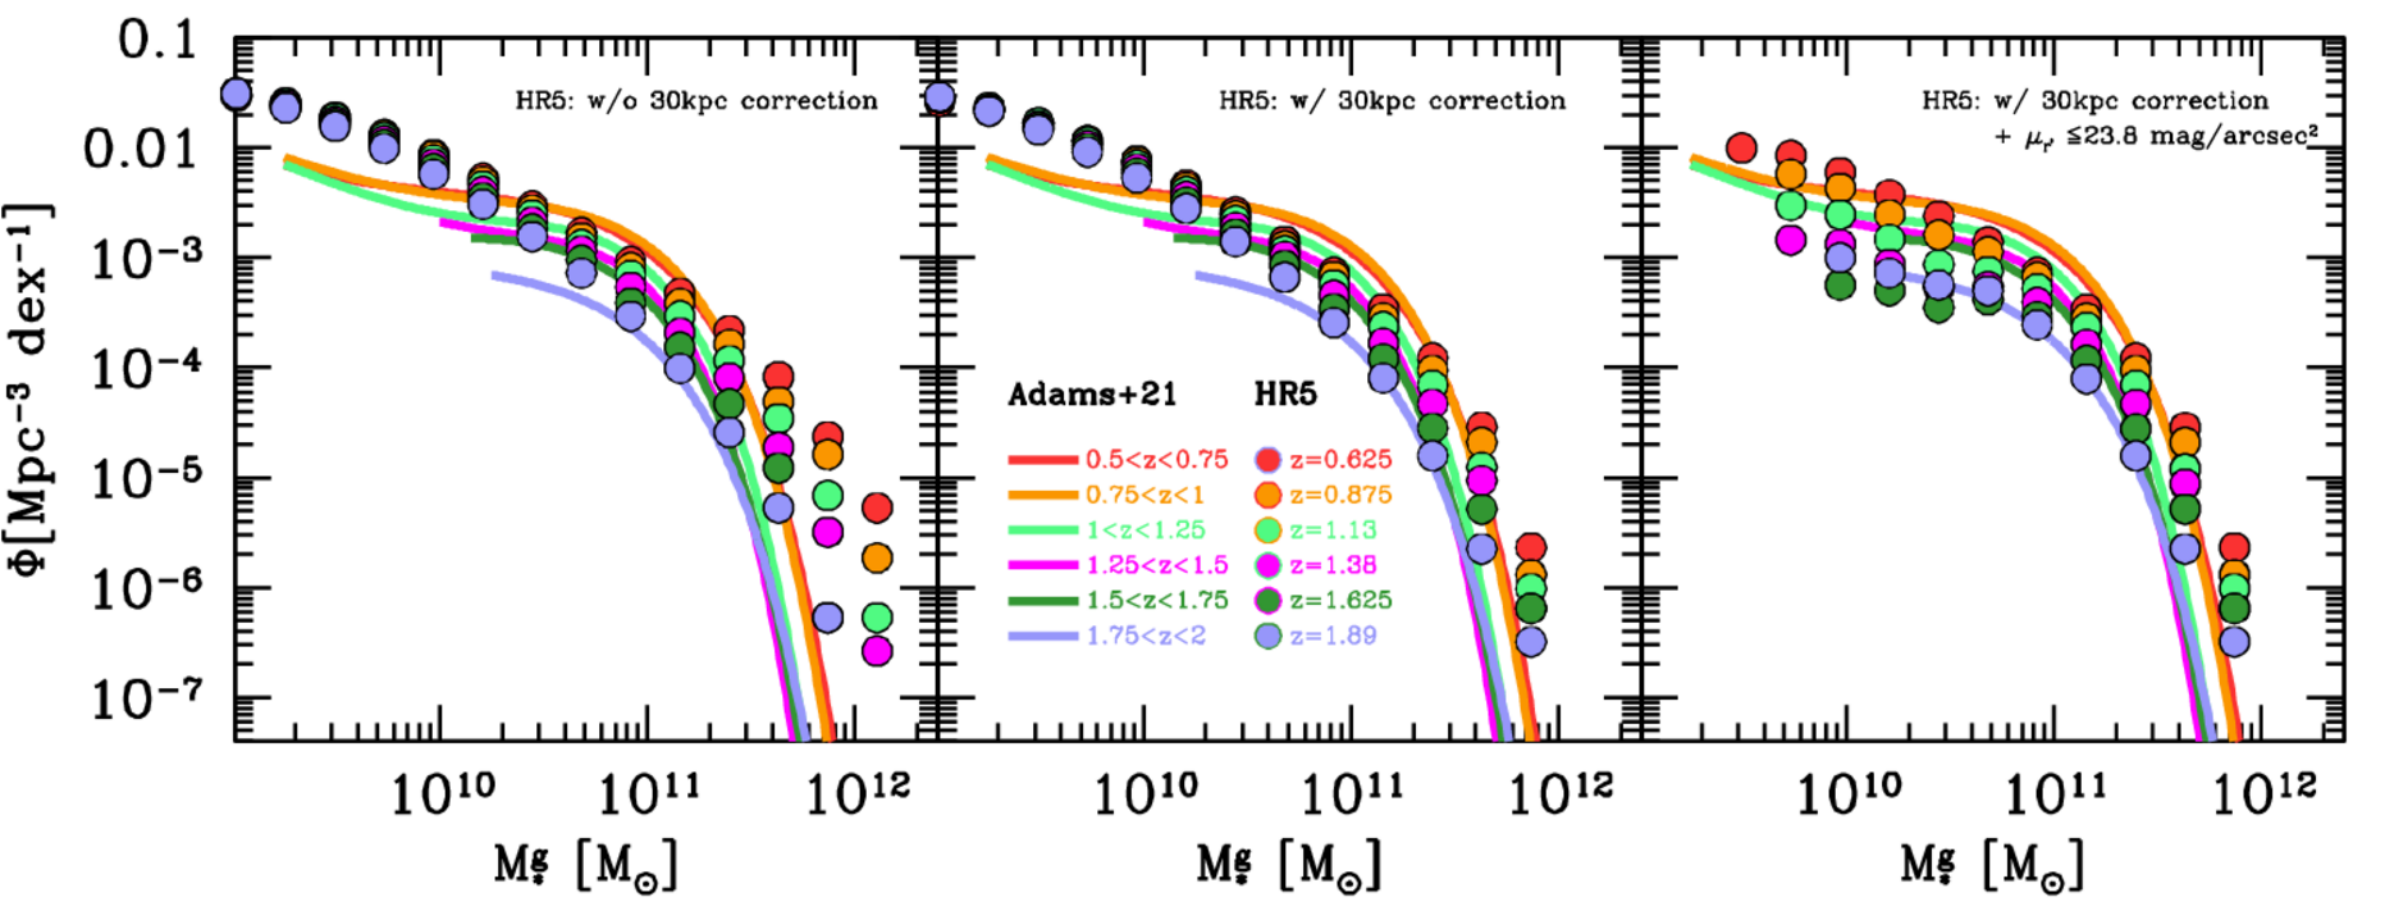
\includegraphics[width=\textwidth]{hr5_gsmf_sblimit.png}
\caption{The low-surface-brightness population missing from the observed galaxy stellar mass function, from the mission team's Horizon Run 5 simulation \cite{kim2023gsmf}. Symbols are simulated mass functions at $z=0.625$--$1.89$, lines the observed functions of Adams et~al.\ \cite{adams2021} in matching bins. \emph{Left}: the raw simulation overproduces low-mass galaxies. \emph{Middle}: measuring simulated masses in the observational $30$\,kpc aperture corrects the massive end. \emph{Right}: additionally imposing the observational surface-brightness limit, $\mu_{r'}\leq23.8$ mag\,arcsec$^{-2}$, removes the low-mass excess, showing the disagreement traces unseen galaxies rather than feedback physics. [reproduced from Kim et~al.\ 2023 \cite{kim2023gsmf}]}
\label{fig:hr5gsmf}
\end{figure}

\subsubsection{Intracluster Light as a Luminous Tracer of Dark Matter}

The second and complementary LSB tracer is the intracluster light (ICL). The ICL is the diffuse stellar component built from stars stripped from galaxies during the hierarchical assembly of the cluster. Those stars are bound to the cluster potential rather than to any single galaxy. Because they are collisionless test particles that have phase-mixed in the global potential, their spatial distribution should follow the total mass. Stacked-cluster photometry first established the ICL as a measurable component at the $\sim10$--$20\%$ level of the total cluster light \cite{zibetti2005}. The decisive result for dark matter is that the projected shape of the ICL closely follows the mass distribution reconstructed from gravitational lensing. In the Hubble Frontier Fields clusters, the ICL isocontours trace the lensing mass contours out to radii of $\sim140$\,kpc more faithfully than the X-ray-emitting gas does \cite{montes2019icl}. That makes the ICL the most accessible luminous tracer of the two-dimensional dark matter distribution in clusters. It offers a cheap, purely photometric route to mapping cluster dark matter on scales and for cluster samples far larger than strong lensing can reach, provided the diffuse light can be measured to $\mu\gtrsim29$ mag\,arcsec$^{-2}$ over the full cluster extent.

A space-based wide-field instrument adds two things to ICL science beyond imaging depth. First, the stable PSF and the absence of airglow allow the diffuse light to be separated cleanly from the wings of bright cluster members, the dominant systematic in ICL photometry. Second, slitless spectroscopy provides discrete dynamical tracers of the same diffuse potential. These are the intracluster planetary nebulae, identifiable by their unresolved [O\,\textsc{iii}]\,$\lambda5007$ emission, and the brighter intracluster globular clusters. Individual line-of-sight velocities at $\sim300$ km\,s$^{-1}$ resolution cannot resolve the internal motions of these tracers. The \emph{ensemble} velocity field of hundreds of intracluster planetary nebulae across a cluster, however, constrains the diffuse-light kinematics. It tests whether the ICL and the dark matter share the same dynamical state \cite{montes2022review}.

\subsubsection{Why Diffuse Light Follows the Dark Matter}

The reason the intracluster light is a good mass tracer, while the X-ray gas is not, is dynamical. Intracluster stars are stripped from their parent galaxies during infall and tidal interactions. They then move as collisionless test particles in the global cluster potential. Violent relaxation and phase mixing distribute them according to the total gravitational field, dark matter included. The hot intracluster gas, by contrast, is collisional and pressure-supported. Therefore, its distribution is shaped by shocks, sloshing, cooling, and active-galactic-nucleus feedback. During a merger it lags and offsets from the collisionless mass, as the Bullet Cluster makes vivid. The empirical result that the ICL isophotes track the lensing mass more tightly than the X-ray isophotes out to $\sim140$\,kpc is the macroscopic expression of this difference \cite{montes2019icl}. The diffuse light therefore offers a two-dimensional, purely photometric reconstruction of the projected dark-matter shape that can be obtained for far larger cluster samples than strong lensing permits and at higher spatial fidelity than X-ray or Sunyaev--Zel'dovich maps.

The diffuse light encodes assembly history as well as shape. The ICL fraction rises with cluster mass and with dynamical age. The radial color and metallicity gradients of the ICL record the masses and infall times of the galaxies that were disrupted to build it. Deep multi-band photometry of the diffuse component therefore constrains when and how the cluster assembled its mass \cite{montes2022review}. A second, discrete tracer is available in the globular-cluster systems of the cluster galaxies and of the UDGs themselves. The number of globular clusters correlates almost linearly with host halo mass. Hence, globular-cluster counts provide a photometric halo-mass estimate independent of stellar luminosity. This is exactly the diagnostic that flagged Dragonfly\,44 as unusually massive (about a hundred globular clusters) and NGC\,1052--DF2 and DF4 as anomalous. Over a full cluster it yields a halo-mass-weighted map of the substructure that complements the smooth ICL.

\subsubsection{Ultra-Diffuse Galaxy Formation and What the Census Decides}

The UDGs are not a single phenomenon. The competing formation channels make distinct, testable predictions that a uniform cluster census can separate. In the ``failed galaxy'' picture, UDGs are objects that formed in relatively massive halos but quenched early, retaining large sizes, old red stellar populations, rich globular-cluster systems, and high dark-matter fractions. In the feedback picture, they are ordinary dwarfs whose stellar bodies were puffed up by episodic gas outflows, predicting younger populations, lower dark-matter fractions, and a link to the dwarf mass--size relation \cite{dicintio2017}. In the high-spin picture, they form in dwarf-mass halos with anomalously high angular momentum, which spreads the disk to low surface brightness without changing the halo mass \cite{amorisco2016}. Tidal interactions in the cluster can additionally transform and further diffuse infalling dwarfs. These channels differ in the predicted abundance of UDGs as a function of cluster mass, their radial distribution within the cluster, their globular-cluster richness, their stellar ages and metallicities, and their dark-matter content, including the existence of the dark-matter-deficient tail. No single object decides between them. A homogeneous sample spanning many clusters of different mass, with structural parameters, stellar-population estimates, and globular-cluster counts measured uniformly, does.

The same wide, deep fields that measure the diffuse light and the UDGs also contain a dense background of faint emission-line galaxies whose shapes can be used for weak-lensing mass reconstruction of the foreground cluster. Because the slitless data supply spectroscopic or grism redshifts for a fraction of these background sources, the lensing kernel is calibrated internally. The lensing mass map can be compared directly, in the same field and on the same astrometric frame, with the ICL-derived luminous tracer. This internal cross-check between an independent gravitational mass map and the diffuse-light tracer is what turns ``the ICL follows the mass'' from a calibrated assumption into a measurement for each individual cluster.

\subsubsection{Cluster-Scale Tests of Dark-Matter Self-Interaction}

Clusters are the highest-velocity ``particle colliders'' available for dark matter. They complement the low-velocity dwarfs of Section~\ref{sec:dwarfvoid} and probe the \emph{velocity dependence} of any self-interaction. Two cluster observables bear directly on the self-interaction cross section. Both work by comparing collisionless tracers with the collisional gas. The first is the spatial offset between components in merging clusters. In a collision the galaxies and the dark matter, being effectively collisionless, pass through one another while the gas is shocked and lags behind. The Bullet Cluster showed the lensing mass leading the X-ray gas, a direct demonstration that the dominant mass is collisionless \cite{clowe2006}. Measuring the small residual offset between the collisionless stellar component and the lensing mass across a sample of merging clusters bounds the momentum exchange of dark matter, currently giving $\sigma/m\lesssim0.5$ cm$^2$\,g$^{-1}$ at cluster collision velocities \cite{harvey2015}. The second observable is the central shape and density of relaxed cluster halos. Self-interactions make the inner halo rounder and reduce its central density. Therefore, the ellipticity and core size of the mass distribution constrain $\sigma/m$ \cite{peter2013}.

The mission supplies the collisionless luminous tracers that both tests require, at higher fidelity than before. The intracluster light and the member-galaxy distribution are the collisionless components whose centroids and shapes must be compared with the lensing mass and the X-ray gas. The deep, space-stable diffuse-light measurement pins the stellar centroid and the halo ellipticity far more accurately than the handful of bright galaxies used in early offset studies. Combined with the dwarf-scale constraints of Section~\ref{sec:dwarfvoid}, a cluster-scale measurement of the same cross section maps $\sigma/m$ across roughly two decades in collision velocity from tens of km\,s$^{-1}$ in dwarfs to thousands in clusters. That velocity span is what tests velocity-dependent self-interaction models rather than a single number. Figure~\ref{fig:sidmsigmav} shows the current state of that measurement. The dwarf and low-surface-brightness galaxies prefer $\sigma/m\simeq2$\,cm$^2$\,g$^{-1}$ while the clusters prefer $\sigma/m\simeq0.1$\,cm$^2$\,g$^{-1}$, a factor-of-twenty velocity dependence inferred from heterogeneous archival samples \cite{kaplinghat2016}. The predicted halo shapes, central densities, and merger offsets for each cross section are produced by the mission team's companion self-interacting-dark-matter simulations and confronted directly with the ICL- and lensing-derived maps.

\begin{figure}[tp]
\centering
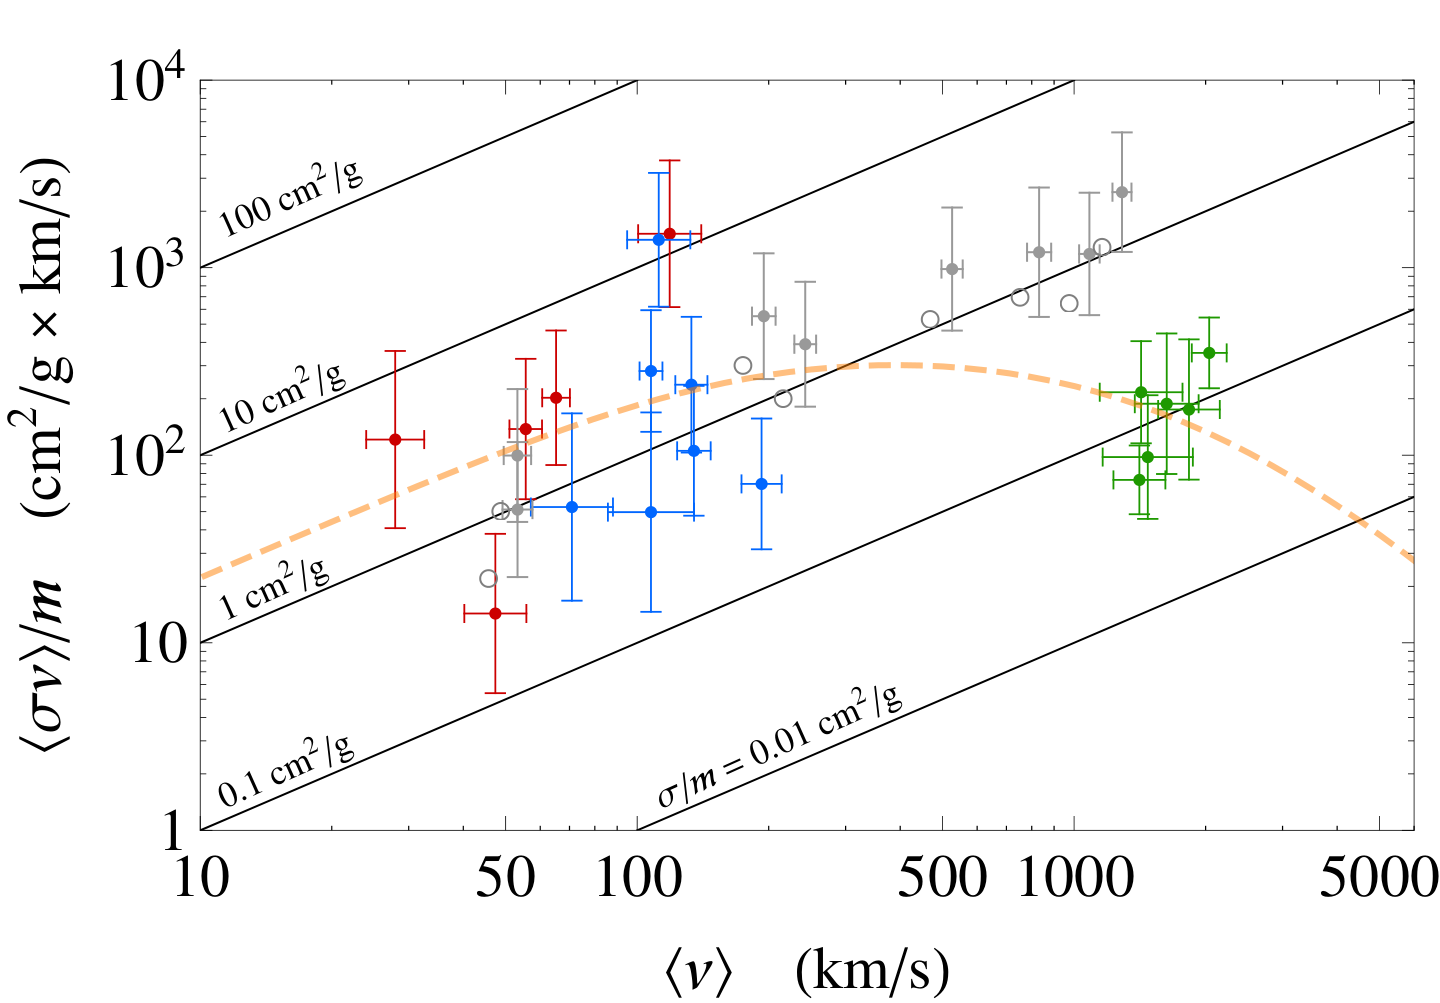
\includegraphics[width=0.62\textwidth]{sidm_sigmav.png}
\caption{The dark-matter self-interaction cross section inferred from astrophysical systems, given as the velocity-weighted cross section per unit mass against the mean collision velocity for dwarf galaxies (red), low-surface-brightness galaxies (blue), and galaxy clusters (green), with SIDM N-body halos simulated at $\sigma/m=1$\,cm$^2$\,g$^{-1}$ (gray), contours of constant $\sigma/m$ (diagonal lines), and the authors' best-fit velocity-dependent dark-photon model (dashed). The downward trend from the dwarf to the cluster regime is the velocity dependence that the mission measures with uniform samples at both ends through the dwarf census of Section~\ref{sec:dwarfvoid} and the cluster merger offsets and halo shapes of this section. [courtesy: Kaplinghat, Tulin \& Yu 2016 \cite{kaplinghat2016}]}
\label{fig:sidmsigmav}
\end{figure}

\subsubsection{Depth, Cadence, and the Cluster Sample}

The defining advantage of the platform for this program is that the surface-brightness limit improves with integration time essentially without the systematic floor that halts ground-based diffuse photometry. With no airglow and a stable photometric response, the noise in a stacked image continues to fall as the square root of exposure until it reaches the astrophysical foreground set by Galactic cirrus and zodiacal light. Hence, reaching $\mu\sim29$--$30$ mag\,arcsec$^{-2}$ is a matter of accumulating exposure rather than of defeating a fluctuating sky. The multi-orientation observing strategy adopted for the flagship survey is doubly valuable here. Rotating the field between visits averages down flat-field residuals and the azimuthal structure of the scattered-light wings of bright stars and galaxies, the dominant systematics in any diffuse-light measurement. A single deep stare cannot do that. A target list of $\sim20$--$40$ clusters at $0.02\lesssim z\lesssim0.10$ matches the field of view to the cluster virial extent. It places the UDG population at sizes that are cleanly resolved and keeps the ICL within reach of the surface-brightness limit out to several hundred kiloparsecs. Spread over the mission lifetime as a deep companion to the wide survey, each cluster receives long multi-roll integrations. The sample spans the cluster-mass range needed to test the predicted scaling of UDG abundance and ICL fraction with halo mass.

\subsubsection{Intracluster Planetary Nebulae and Globular Clusters as Discrete Tracers}

The slitless mode turns the diffuse light into a dynamical tracer through two populations of compact objects that a grism survey detects naturally. Intracluster planetary nebulae radiate almost all of their light in the [O\,\textsc{iii}]\,$\lambda5007$ line and have negligible continuum. Therefore, they appear in a slitless survey as pure emission-line point sources, exactly the kind of object the instrument is optimized to find. Hundreds to thousands of them populate a nearby cluster. Although the $300$\,km\,s$^{-1}$ resolution element does not resolve the motion of a single planetary nebula precisely, the relevant dynamical signal here is the cluster-scale velocity field, whose dispersion of $500$--$1000$\,km\,s$^{-1}$ is comfortably larger than the resolution. With adequate signal-to-noise on the bright line the per-object velocity is recovered to well within the cluster dispersion. Hence, the \emph{ensemble} line-of-sight velocity distribution of the intracluster planetary nebulae measures the kinematics of the diffuse stellar component directly. This tests whether the intracluster light and the dark matter share the same dynamical state and not merely the same projected shape. It extends the mass profile to large radii where lensing and X-ray data weaken. The planetary-nebula luminosity function additionally provides an independent distance to each cluster, anchoring the photometry \cite{montes2022review}.

The second population is the globular clusters. The total number of globular clusters in a galaxy correlates nearly linearly with its host halo mass over several decades, making globular-cluster counts a photometric halo-mass estimator that is independent of the diffuse stellar luminosity \cite{harris2013}. Applied across a cluster, this yields a halo-mass-weighted map of the surviving substructure. Applied to individual UDGs it provides the halo masses that, in combination with the stellar kinematics measured by high-resolution follow-up, flag the dark-matter-rich and dark-matter-deficient extremes. The intracluster globular clusters which have been stripped into the general cluster potential trace the same diffuse halo as the intracluster light, giving a discrete spatial tracer to complement the continuous surface-brightness map. Both populations are by-products of the same deep imaging and slitless spectroscopy taken for the diffuse-light and UDG science and, therefore, they add dynamical information at no extra observational cost.

\subsubsection{The Diffuse Light to the Halo Edge and the Splashback Radius}

The dark-matter content of a cluster is encoded not only in the shape of the inner mass distribution but in the extent and slope of its outskirts. Here too the diffuse light is the accessible tracer. Cold dark matter predicts a physical halo boundary, the splashback radius, marking the apocenter of material on its first orbit after collapse, beyond which the mean density profile steepens abruptly. The location of this feature is set by the recent mass-accretion rate and therefore by the growth of structure \cite{more2015}. The splashback radius has been detected statistically in the radial profile of satellite galaxies around massive clusters \cite{more2016}. Because the intracluster light and the satellite galaxies are both collisionless tracers of the same potential, mapping their profiles to large radius locates the feature and measures the cluster accretion rate. This is a measurement of the dark-matter distribution at the halo edge that complements the core-focused lensing and ICL-shape analyses. It is sensitive to the dark-matter model. Warm, fuzzy, and self-interacting variants modify the abundance and survival of the infalling substructure that defines the splashback transition.

Reaching this regime requires diffuse-light photometry to $\mu\sim30$ mag\,arcsec$^{-2}$ over the full virial extent and into the infall region at several megaparsecs, a combination of depth and contiguous area that ground-based facilities achieve only with great difficulty against their fluctuating sky. The platform's stable response and airglow-free background, together with the wide field tiled across the cluster outskirts, make the outer ICL profile and the radial distribution of faint member galaxies measurable in the same data set. Hence, the splashback feature and the cluster assembly history come essentially for free alongside the core mapping. Combined with the inner ICL shape, the merger offsets, and the globular-cluster and planetary-nebula dynamics, the result is a dark-matter map of each cluster spanning from the core to the accretion boundary.

\subsubsection{Observing Strategy and Survey Reach}

The LSB cluster program is a deep, targeted use of the wide field rather than a blind survey. The adopted plan targets a sample of $\sim20$--$40$ nearby clusters at $0.02\lesssim z\lesssim0.10$, where UDGs are spatially resolved and the ICL fills a large fraction of the field. Long multi-orientation integrations per cluster reach a $1\sigma$ surface-brightness limit of $\mu\sim29$--$30$ mag\,arcsec$^{-2}$ in the stacked image. Table~\ref{tab:lsbreach} summarizes the planning reach. The same exposures yield the slitless spectra of compact emission-line tracers (intracluster planetary nebulae, background emission-line galaxies for weak-lensing shape calibration) and of any star-forming LSB dwarfs. Table~\ref{tab:lsbanchors} places the published measurements that anchor each scientific claim of the program next to the capability the mission adds to it.

\begin{table}[tp]
\centering
\sffamily\small
\begin{tabularx}{\textwidth}{@{}p{3.6cm}p{3.2cm}X@{}}
\toprule
\textbf{Product} & \textbf{Planning depth} & \textbf{Dark-matter use}\\
\midrule
UDG photometric census & $\mu(g)\sim30$ mag\,arcsec$^{-2}$, $r_{\rm e}\gtrsim1$\,kpc & Abundance, radial distribution, structural diversity in the host potential, and the DM-rich versus DM-free fraction\\
Intracluster light map & $\mu\sim29$--$30$ mag\,arcsec$^{-2}$ to $\gtrsim300$\,kpc & Two-dimensional luminous tracer of the projected total-mass (dark matter) distribution\\
Compact dynamical tracers & [O\,\textsc{iii}] PNe, intracluster GCs & Ensemble velocity field of the diffuse component and consistency of light and mass\\
\bottomrule
\end{tabularx}
\caption{Planning reach of the low-surface-brightness cluster program. Internal stellar velocity dispersions of individual UDGs (a few to tens of km\,s$^{-1}$) are below the $R=1000$ resolution element and require high-resolution follow-up. The mission supplies the wide-field deep census, the ICL map, and the ensemble kinematics of compact tracers.}
\label{tab:lsbreach}
\end{table}

\begin{table}[tp]
\centering
\sffamily\small
\begin{tabularx}{\textwidth}{@{}p{2.6cm}p{5.6cm}X@{}}
\toprule
\textbf{Observable} & \textbf{Published anchor} & \textbf{What the mission adds}\\
\midrule
UDG abundance & 47 Coma UDGs from Dragonfly \cite{vandokkum2015coma}, expanded to $\sim\!10^3$ by Subaru imaging \cite{koda2015,yagi2016} & One uniform census across $\sim$20--40 clusters to $\mu(g)\sim30$ mag\,arcsec$^{-2}$\\
UDG dark-matter extremes & DF44 with $\sigma\simeq47$ km\,s$^{-1}$ and $\sim$100 globular clusters \cite{vandokkum2016df44} against DF2/DF4 with $\sigma\simeq3$--$4$ km\,s$^{-1}$ \cite{vandokkum2018df2,vandokkum2019df4} & Globular-cluster counts and membership over whole clusters that select both extremes for kinematic follow-up\\
ICL fraction & 10--20\% of the total cluster light in stacked photometry \cite{zibetti2005} & Per-cluster ICL maps to $\mu\sim29$--$30$ mag\,arcsec$^{-2}$ beyond $300$ kpc\\
ICL as mass tracer & ICL isocontours follow the lensing mass to $\sim$140 kpc in the Frontier Fields \cite{montes2019icl} & The same test repeated cluster by cluster against internally calibrated weak lensing\\
SIDM cross section & $\sigma/m\lesssim0.5$ cm$^2$\,g$^{-1}$ from stellar--lensing offsets in merging clusters \cite{harvey2015} & Deep ICL centroids and halo ellipticities for much larger merger samples\\
Halo edge & Splashback radius detected statistically in stacked satellite profiles \cite{more2016} & Diffuse light and satellites traced to the boundary of individual clusters\\
Depth ceiling & Ground limits $\mu\sim28$--$29$, Dragonfly $\mu\sim30$--$31$ mag\,arcsec$^{-2}$ \cite{abraham2014dragonfly} & ETC reach $\mu_{5\sigma}(10'')=28.9$--$31.9$ for $0.25$--$64$ hr (Figure~\ref{fig:iclimg})\\
\bottomrule
\end{tabularx}
\caption{Published measurements that anchor the cluster low-surface-brightness program, placed next to the step the mission adds to each. Every quantitative claim of the program traces back to one of these anchors.}
\label{tab:lsbanchors}
\end{table}

The exposure-time calculator sets the surface-brightness reach directly. Figure~\ref{fig:icl} gives the time to a $5\sigma$ detection of intracluster light binned over a $10\times10$\,arcsec$^2$ region as a function of cluster redshift, including the $(1+z)^4$ cosmological surface-brightness dimming that dominates the trend. A rest-frame $\mu\simeq26$\,AB\,arcsec$^{-2}$ envelope is reached in about a minute to $z\simeq0.3$ and the fainter $\mu\simeq28$ outskirts in about an hour. Therefore, the diffuse light can be traced toward the cluster edge across the sample.

\begin{figure}[tp]
\centering

\includegraphics[width=0.7\textwidth]{icl_exptime_vs_z.png}
\caption{Exposure to a $5\sigma$ detection of intracluster light over a $10\times10$\,arcsec$^2$ bin versus cluster redshift in the $H$ band for four rest-frame surface brightnesses, including the $(1+z)^4$ dimming. The $1$\,hr level is marked.}
\label{fig:icl}
\end{figure}

A dedicated deep pointing on a single cluster turns this reach into a direct image. Figure~\ref{fig:iclimg} takes the deep HST Frontier Fields WFC3/IR F160W mosaic of Abell~2744 \cite{lotz2017} as the true scene and passes it through the same exposure-time calculator, adding the source, sky, dark, and read noise in quadrature to the noise already present in the true scene so that each simulated frame reproduces exactly the ETC per-pixel noise. Four total integrations of a dedicated intracluster-light program are shown, being a quarter of an hour, four, sixteen, and sixty-four hours, reaching $5\sigma$ surface-brightness limits over a $10\times10$\,arcsec$^2$ bin of $\mu\simeq28.9$, $30.4$, $31.2$, and $31.9$\,AB\,arcsec$^{-2}$. Each panel is stretched between a fixed bright limit and its own per-pixel noise floor. Hence, the background tone is common across the four and the eye reads directly how much fainter the diffuse light is traced as the exposure grows. The intracluster envelope that is buried in the noise at a quarter of an hour is mapped smoothly between the cluster galaxies and out to the faint tidal features by sixteen to sixty-four hours. At the longest integrations the reach passes the depth of the space-based Frontier Fields imaging that itself defines the state of the art for cluster diffuse light. That is the concrete sense in which the platform advances intracluster-light science.

\begin{figure}[tp]
\centering
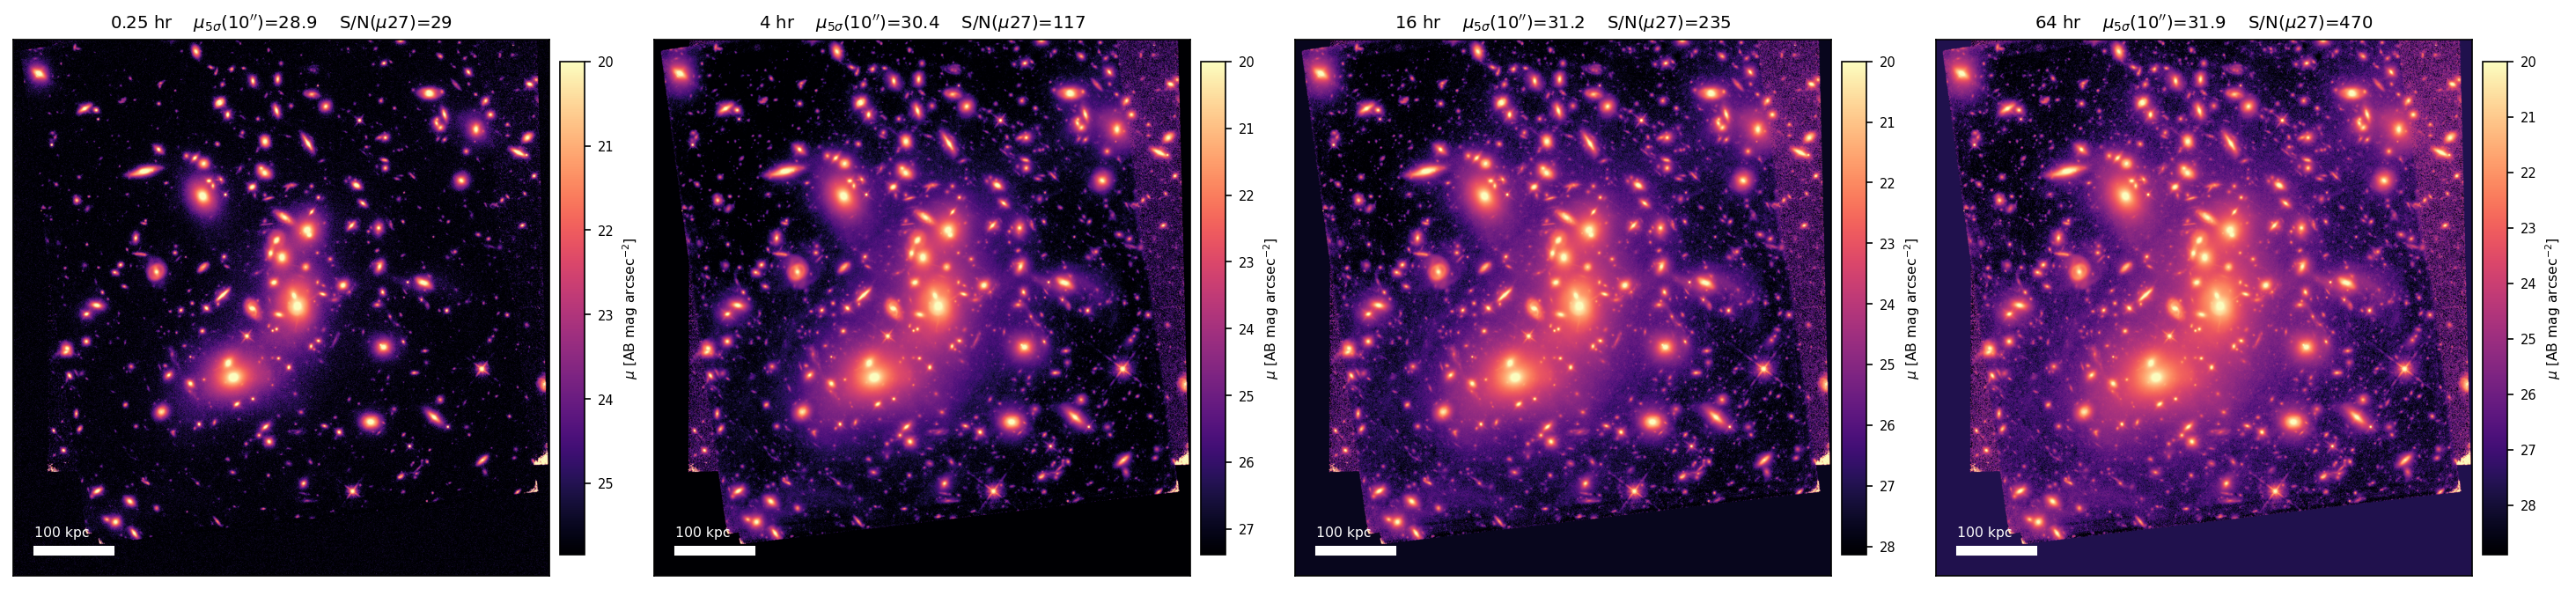
\includegraphics[width=\textwidth]{icl_exposure_demo.png}
\caption{Simulated appearance of the Abell~2744 intracluster light to the 3.5\,m ST vs total exposure time, as a dedicated deep program rather than a wide-survey tier. The deep HST Frontier Fields WFC3/IR F160W mosaic \cite{lotz2017} is the true scene ($z=0.308$, observed $H$ band). For each exposure the ETC source, sky, dark, and read noise are added in quadrature to the noise already present in the truth image. Therefore, the displayed per-pixel noise equals the ETC prediction. The annotated signal-to-noise is the ETC value for a $\mu=27$\,AB\,arcsec$^{-2}$ patch over a $10\times10$\,arcsec$^2$ box. Each panel is stretched between a fixed bright limit and its own $1\sigma$ per-pixel noise floor. Hence, the growth of traceable diffuse light with exposure is directly visible. Each panel has its own colour bar and a $100$\,kpc scale bar.}
\label{fig:iclimg}
\end{figure}

\subsubsection{Program Scope and Synergy}

The program is scoped as a cluster-dark-matter mapping and LSB-census effort. The deliverables are a uniform UDG catalog with structural parameters and stellar-population estimates across the target clusters, deep ICL maps that serve as luminous dark-matter tracers for cross-comparison with weak- and strong-lensing mass reconstructions, and a sample of intracluster compact emission-line tracers for ensemble dynamics. The natural external synergies are with Euclid and Rubin/LSST, which provide the wide but shallower imaging that selects target clusters, feeding weak-lensing mass maps. Internally the strong-lens program of Section~\ref{sec:stronglens} supplies the mass models that serve as an independent reference for the ICL-as-tracer hypothesis. High-resolution spectroscopy from large ground-based telescopes remains the source of individual UDG velocity dispersions. The mission's role is the deep, wide, space-stable diffuse-light measurement that no ground-based facility can match. Taken together, the inner ICL shape compared against lensing, the merger offsets of the collisionless stellar component, the globular-cluster and planetary-nebula dynamics, and the outer profile to the splashback radius constitute a dark-matter map of each target cluster from the core to the accretion boundary. The self-interaction cross section at cluster velocities comes with it, complementing the dwarf-scale measurement. The concrete deliverables are the following.
\begin{itemize}[leftmargin=1.4em,itemsep=1pt,topsep=2pt]
\item A uniform ultra-diffuse-galaxy catalog across $\sim20$--$40$ clusters with structural parameters, stellar-population estimates, and globular-cluster counts.
\item A field LSBG and UDG catalog over the full $100$--$300$\,deg$^2$ wide footprint to $\mu_{5\sigma}(10'')\simeq29.8$--$31.3$ in $g$ (Table~\ref{tab:lsbsurvey}) with slitless redshifts, physical sizes, and survey-internal environments for the emission-line subset.
\item Deep intracluster-light maps to $\mu\sim29$--$30$ mag\,arcsec$^{-2}$ serving as luminous tracers of the projected dark-matter distribution from the core to the splashback radius.
\item Collisionless-tracer centroids and shapes for merger-offset and halo-ellipticity constraints on $\sigma/m$ at cluster velocities.
\item Ensemble kinematics of intracluster planetary nebulae and globular clusters for the diffuse-component dynamics.
\item Internal cross-checks against weak- and strong-lensing mass maps built from background sources in the same fields.
\end{itemize}

\subsection{Dwarf and Void Galaxies: Testing the Particle Nature of Dark Matter}\label{sec:dwarfvoid}

Dwarf galaxies are the smallest gravitationally bound stellar systems known and the most dark-matter-dominated, with dynamical mass-to-light ratios of hundreds to thousands in the faintest Milky Way satellites. Their shallow potentials and low star-formation efficiencies make them maximally sensitive to the microphysics of dark matter and to the baryonic feedback that competes with it. Cosmic voids, the underdense regions that occupy most of the volume of the Universe, sharpen this test further, since the dwarfs and dark galaxies found there have assembled in near-isolation, free of the mergers, ram pressure, and tidal harassment that reshape galaxies in denser environments and that can mimic a dark-sector signal. This program is a wide-field search for dwarf and dark galaxies across field, group, cluster, and void environments, designed to build the uniform, environment-spanning samples on which the small-scale tests of cold, self-interacting, and fuzzy dark matter depend.

\subsubsection{Dwarfs as Dark-Matter Laboratories}

The dark-matter content of a pressure-supported dwarf is measured from the line-of-sight stellar velocity dispersion $\sigma_{\rm los}$ and the projected half-light radius $r_{1/2}$ through the mass estimator
\begin{equation}
M_{1/2}=\frac{4\,\sigma_{\rm los}^2\,r_{1/2}}{G}\simeq930\left(\frac{\sigma_{\rm los}}{\rm km\,s^{-1}}\right)^{2}\!\left(\frac{r_{1/2}}{\rm pc}\right)M_\odot,
\label{eq:wolf}
\end{equation}
which is robust to the unknown velocity anisotropy because it is evaluated at the half-light radius \cite{wolf2010}. Applied to the classical and ultra-faint dwarf spheroidals \cite{mateo1998}, Eq.~\eqref{eq:wolf} yields masses that exceed the stellar mass by one to four orders of magnitude. The ultra-faint dwarfs in particular, with luminosities as low as a few hundred $L_\odot$ and velocity dispersions of $2$--$10$ km\,s$^{-1}$, are the cleanest probes of the halo mass function and inner density structure at the smallest accessible scales \cite{simon2019}. Their abundance, radial distribution, and internal densities each encode a different aspect of the dark-matter model.

\subsubsection{Small-Scale Challenges to Cold Dark Matter}

Collisionless cold dark matter (CDM) reproduces the observed Universe on large scales but faces a set of persistent tensions on dwarf-galaxy scales, reviewed comprehensively by \cite{bullock2017}. The \emph{core--cusp} problem is the mismatch between the steep central density cusps, $\rho\propto r^{-1}$, predicted by dissipationless CDM simulations and the shallower, cored profiles inferred from the rotation curves and stellar kinematics of many dwarfs \cite{deblok2010}. The \emph{missing-satellites} problem is the order-of-magnitude excess of predicted subhalos over observed satellites \cite{moore1999}. The \emph{too-big-to-fail} problem is the observation that the densest predicted subhalos are too centrally dense to host the observed bright satellites \cite{boylankolchin2011}. Most sharply, the \emph{diversity} problem is the wide scatter in the inner slopes of dwarf rotation curves at fixed maximum circular velocity, with galaxies ranging from strongly cored to cuspy where CDM predicts near-uniformity \cite{oman2015}. Baryonic feedback can plausibly erase cusps in gas-rich dwarfs with extended star formation, but it struggles to explain the gas-poor and ultra-faint regime and the full breadth of the diversity, which keeps open the possibility that the resolution lies in the dark sector itself.

\subsubsection{Self-Interacting and Fuzzy Dark Matter}

Self-interacting dark matter (SIDM) addresses these tensions by endowing dark matter with an elastic self-scattering cross section \cite{spergel2000}. Scattering transports heat into the halo center. The rate per particle, $\Gamma\simeq(\sigma/m)\,\rho\,v_{\rm rms}$, becomes of order one over a Hubble time when $\sigma/m\sim1$ cm$^2$\,g$^{-1}$ at dwarf-halo densities and velocities, naturally forming a constant-density core \cite{tulinyu2018}. Dwarf halos thus act as ``particle colliders''. The inferred core sizes and central densities map directly to the cross section at the corresponding relative velocity, so a velocity-dependent $\sigma/m$ can be reconstructed across systems from dwarfs to clusters \cite{kaplinghat2016}. SIDM also predicts a second, counter-intuitive phase, gravothermal core collapse to a high central density, so that the same physics produces both unusually diffuse and unusually dense dwarfs, a natural explanation of the rotation-curve diversity which uniform CDM does not offer \cite{ren2019}. If dark matter is instead an ultralight boson with $m\sim10^{-22}$\,eV, its de~Broglie wavelength is of kiloparsec scale and wave (``fuzzy'') effects suppress small-scale structure and replace central cusps with solitonic cores \cite{hu2000,schive2014}. The soliton core radius follows a core--halo relation that scales as
\begin{equation}
r_{\rm c}\simeq1.6\;{\rm kpc}\left(\frac{m}{10^{-22}\,\rm eV}\right)^{-1}\!\left(\frac{M_{\rm halo}}{10^{9}\,M_\odot}\right)^{-1/3},
\label{eq:soliton}
\end{equation}
so that dwarf galaxies, with the smallest halo masses, host the largest and most observable cores and set the strongest constraints on the boson mass \cite{schive2014}. Figure~\ref{fig:fdmslice} shows what such a halo looks like in the first cosmological wave-dark-matter simulation, with de~Broglie interference granules pervading the halo and filaments and the solitonic core standing at the center in place of a cusp. Both models make a statistical rather than a single-object prediction. Testing SIDM or FDM requires the \emph{distribution} of central densities and core sizes across a large, uniformly selected sample spanning a range of halo masses and environments, which is what a wide-field census provides and what the mission team's companion SIDM and wave-dark-matter simulations predict for comparison.

Stellar-kinematic analyses of individual dwarfs give boson masses clustering near $m\sim(1$--$6)\times10^{-22}$\,eV \cite{calabrese2016}, shown against the core--halo relation of Eq.~\eqref{eq:soliton} in Figure~\ref{fig:soliton}. These kinematically preferred masses are under pressure from independent probes, compiled in Figure~\ref{fig:fdmconstraints}. The Ly$\alpha$ forest excludes $m<2\times10^{-21}$\,eV even with a conservative thermal history \cite{irsic2017fdm} and $m<2\times10^{-20}$\,eV once the intergalactic thermal history is marginalized \cite{rogers2021}, the Milky Way satellite census requires $m>2.9\times10^{-21}$\,eV \cite{nadler2021}, and the sizes and stellar kinematics of Segue~1 and Segue~2 exclude everything below $3\times10^{-19}$\,eV \cite{dalal2022}. Taken at face value these bounds close the window in which the boson explains the dwarf cores, but they rest on different astrophysical assumptions and different systems from the kinematic preferences. What settles the question is a single uniform dwarf census whose core-size and central-density distributions confront the preferred band directly on the very population that produces it.

\begin{figure}[tp]
\centering
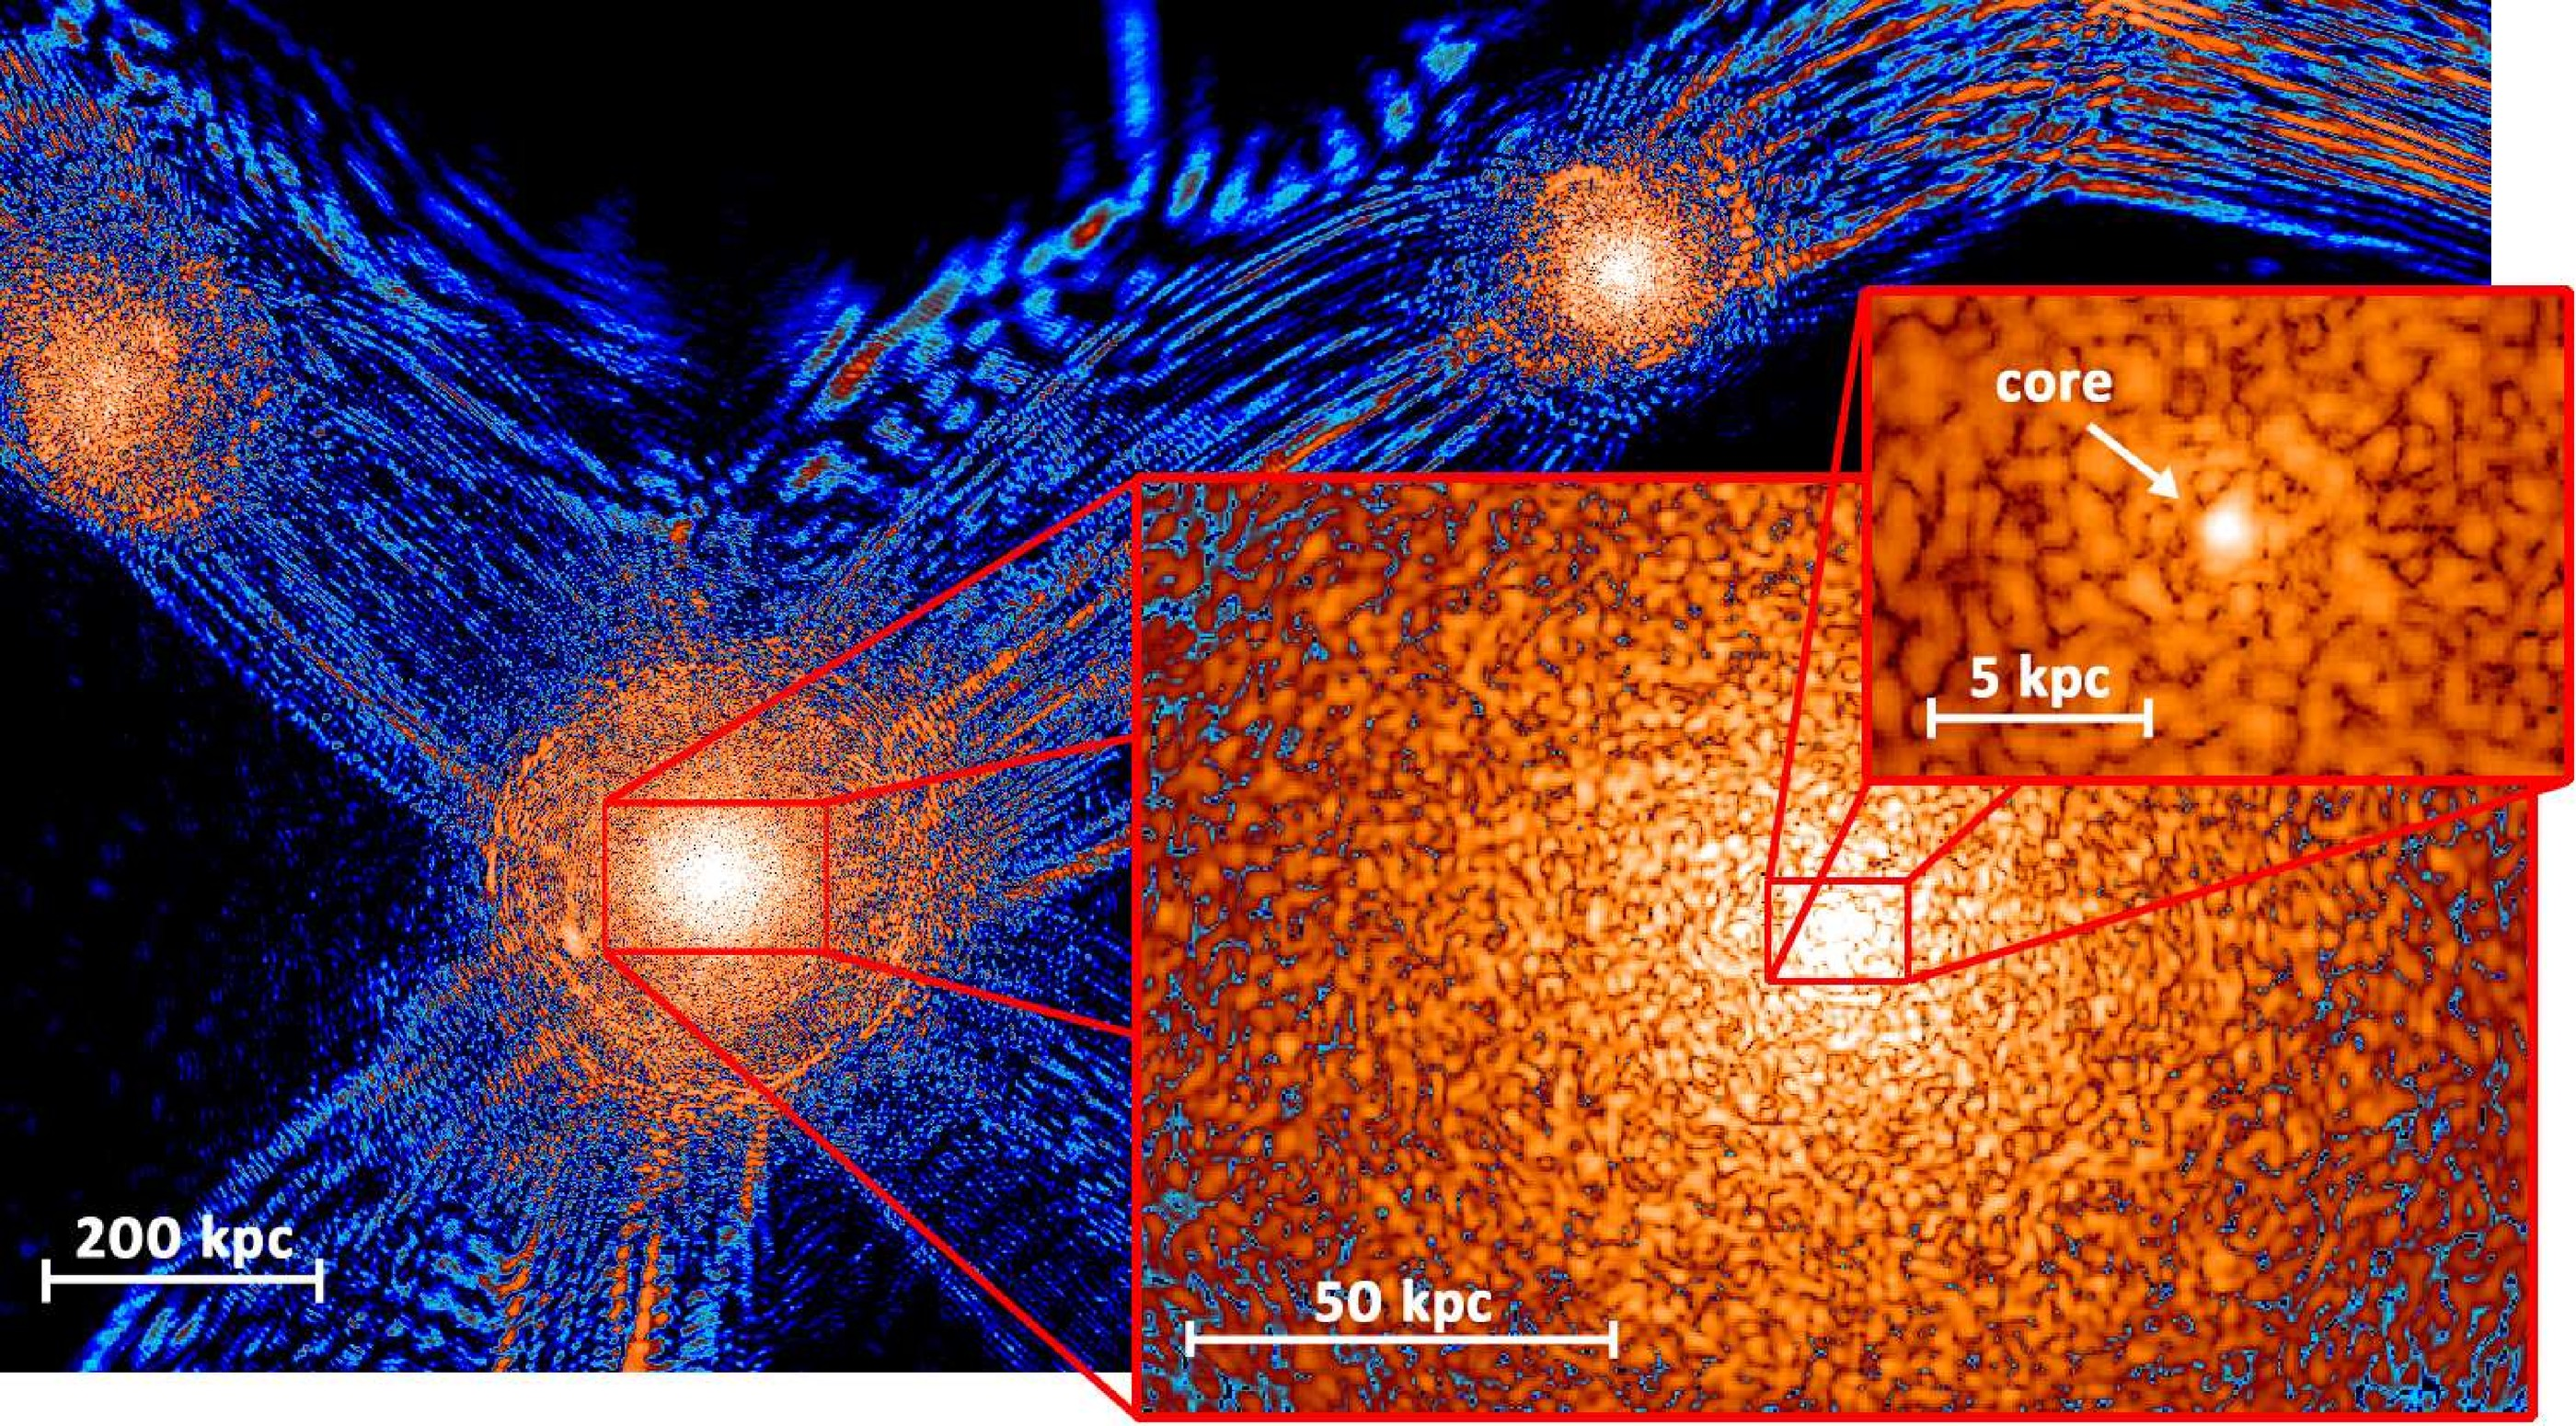
\includegraphics[width=\textwidth]{fdm_wave_slice.jpg}
\caption{A galaxy-scale halo in the first cosmological simulation of wave (fuzzy) dark matter, shown as a density slice with successive zooms. The kiloparsec de~Broglie wavelength of the ultralight boson imprints interference granules and destructive fringes throughout the filaments and the halo. The halo center hosts the distinctive solitonic core of Eq.~\eqref{eq:soliton} rather than a cusp, largest in the smallest halos, the structure the dwarf census tests at the population level. [courtesy: Schive et al. 2014 \cite{schive2014}]}
\label{fig:fdmslice}
\end{figure}

\begin{figure}[tp]
\centering
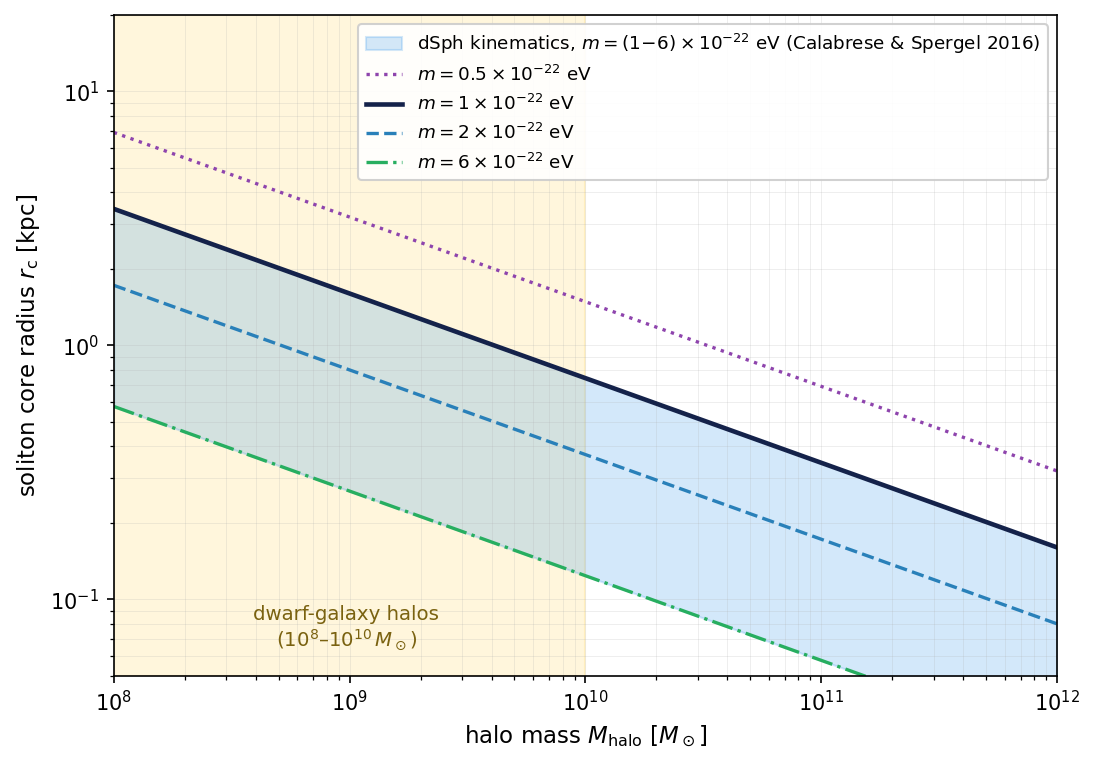
\includegraphics[width=0.72\textwidth]{fdm_soliton_relation.png}
\caption{The published fuzzy-dark-matter core--halo relation of Eq.~\eqref{eq:soliton} \cite{schive2014} at $z=0$ for four boson masses with the band preferred by dwarf-spheroidal kinematics \cite{calabrese2016}. In the dwarf halo-mass range (shaded) the predicted soliton cores reach a substantial fraction of the galaxy size, so the size and central-surface-brightness distributions of a uniform dwarf census constrain the boson mass at the population level.}
\label{fig:soliton}
\end{figure}

\begin{figure}[tp]
\centering
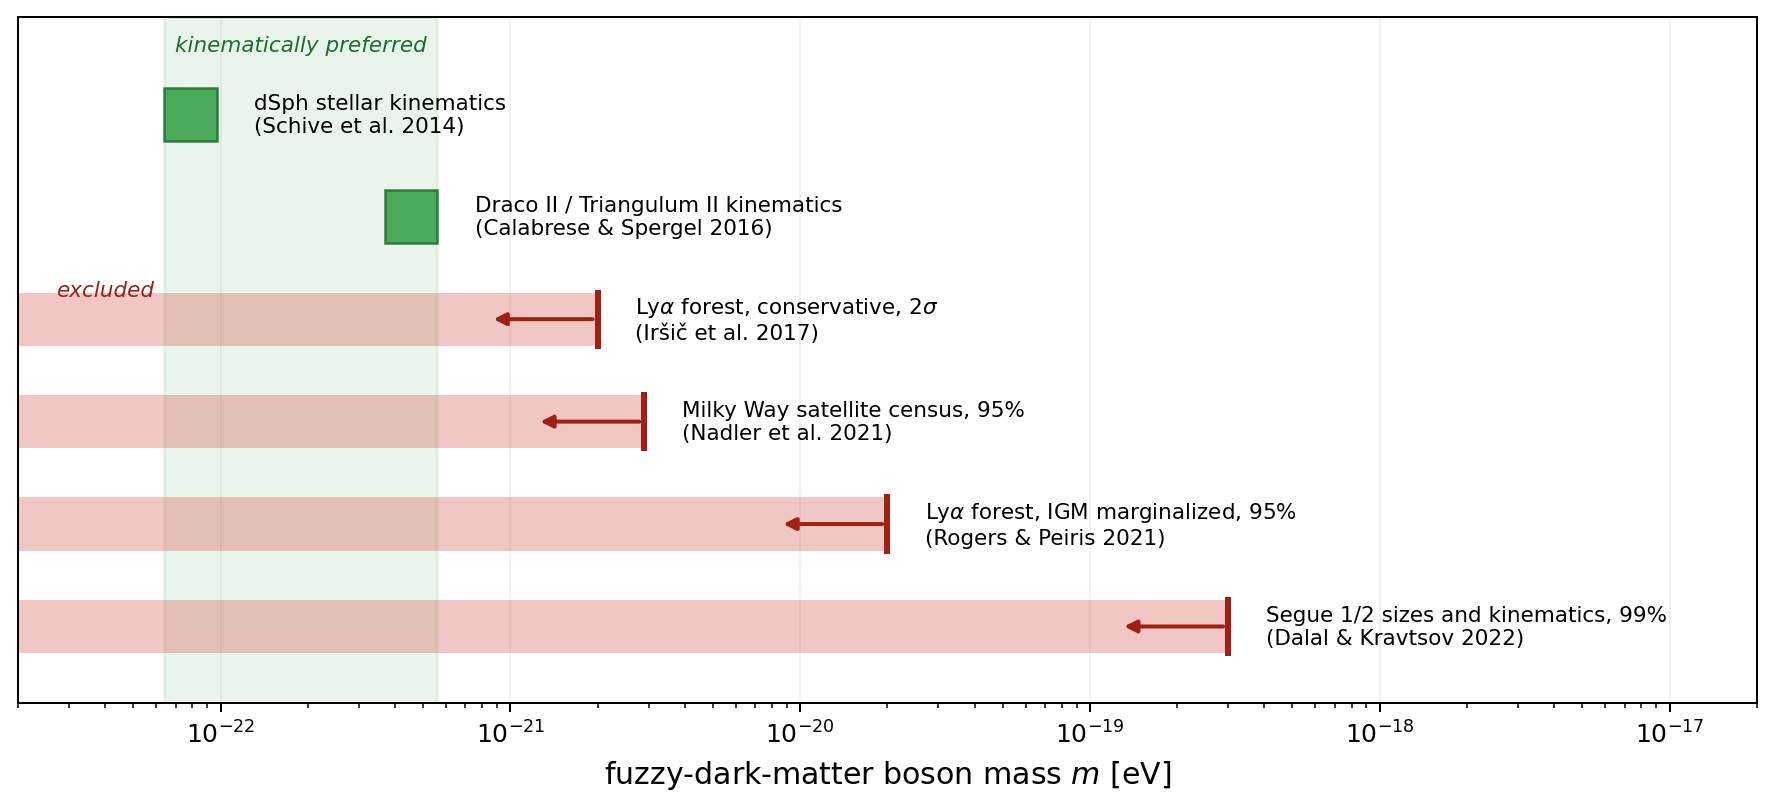
\includegraphics[width=0.78\textwidth]{fdm_mass_constraints.png}
\caption{Published constraints on the fuzzy-dark-matter boson mass, drawn from the quoted papers. Green bands mark the masses preferred by stellar kinematics of dwarf spheroidals \cite{schive2014} and of the ultra-faint dwarfs Draco~II and Triangulum~II \cite{calabrese2016}. Red regions are excluded by the Ly$\alpha$ forest under conservative thermal-history assumptions \cite{irsic2017fdm}, by the Milky Way satellite census \cite{nadler2021}, by the Ly$\alpha$ forest marginalized over the intergalactic thermal history \cite{rogers2021}, and by the sizes and stellar kinematics of Segue~1 and 2 \cite{dalal2022}. The direct conflict between the kinematically preferred band and the exclusion limits is the current state of the field. The uniform core-size census of this survey tests the preferred band on the very population that produces it.}
\label{fig:fdmconstraints}
\end{figure}

\subsubsection{The Halo Mass Function and the Void Phenomenon}\label{sec:voidphenom}

Beyond the inner density structure, the sheer \emph{abundance} of low-mass halos is a sharp discriminant between dark-matter models. Cold dark matter predicts a halo mass function that continues as a power law far below the dwarf scale, whereas warm dark matter truncates it through the free-streaming of a thermal relic and fuzzy dark matter truncates it through the de~Broglie wavelength that suppresses power below a half-mode scale. Both cutoffs land at dwarf and satellite masses for the parameter ranges of current interest. The census of Milky Way satellites already turns this into a quantitative bound, using the observed number and luminosity function of satellites discovered by the Dark Energy Survey and Pan-STARRS, corrected for completeness \cite{nadler2021}. But the satellite measurement is made in the special, tidally violent environment of a massive host. There, self-interacting dark matter, for instance, also accelerates the tidal evaporation and core collapse of subhalos. This alters both their counts and their central densities, entangling the abundance signal with environment.

Voids are the cleanest place to isolate it. Cold dark matter predicts that voids are filled with low-mass halos, yet the observed void galaxy population is sparse and, where present, consists of faint late-type dwarfs, the long-standing ``void phenomenon'' \cite{peebles2001}. Two resolutions are possible, and they point in opposite directions for the nature of dark matter. Either the low-mass halos exist but failed to form stars, because the ultraviolet background and inefficient gas cooling suppressed star formation below a halo-mass threshold of a few $\times10^{9}\,M_\odot$ \cite{hoeft2010}. This would leave voids full of gas-bearing but optically dark or ultra-faint systems still waiting to be found. Or the low-mass halos are themselves suppressed, as warm or fuzzy dark matter would predict. Because a void's underdensity is not replenished by accretion, a small-scale cutoff in the power spectrum shows up there with the least astrophysical contamination and the least tidal confusion. Therefore, the faint-end slope of the void galaxy and H\,\textsc{i} mass functions is among the most direct measurements of low-mass halo abundance available, complementing rather than duplicating the satellite-based bound. Voids are also a cosmological probe in their own right. The abundance, sizes, shapes, and outflow velocities of the galaxies streaming out of them constrain the growth rate of structure, the dark-energy equation of state, and the summed neutrino mass \cite{hamaus2016}. A spectroscopic survey that places accurate redshifts on faint void galaxies therefore improves the geometric definition of the voids and their interior tracer density, while also delivering the dark-matter census.

Figure~\ref{fig:voidwedge} makes the void-search target selection concrete with real data rather than an assumed catalog. It shows the one void of the independent Bayesian catalog of Malandrino et al.\ \cite{malandrino2026} whose center falls inside the flagship Bo\"otes wide spectroscopic tier (Section~\ref{sec:deepfields}), with a published position and redshift rather than an estimate made for this proposal. Its position, redshift, and size match the classic Bo\"otes Void first found by Kirshner et al.\ \cite{kirshner1981,kirshner1987}, one of the largest voids known in the local Universe, independently reconfirmed here by a modern Bayesian void finder applied to SDSS and 2MRS data. Its radius is shown here at one-half of the catalog's quoted mean value, restricting the demonstration to the void's innermost interior so that the classified sample targets genuine void galaxies rather than the wall population that a void-finder radius can otherwise include. The location matters. Void membership needs the same redshift-based three-dimensional position that a UDG classification requires (Section~\ref{sec:lsb}). The imaging-only wide extension and the ultra-deep fields carry no spectroscopy and cannot supply it, while the wide, medium, and deep spectroscopic tiers can. Real SDSS-I/II Main Galaxy Sample spectroscopy over the void's own radial extent, its comoving distance plus and minus its cataloged radius, classifies each galaxy by its true three-dimensional distance from the void center rather than by sky position alone, since a flat sky projection otherwise mixes in galaxies that merely sit in front of or behind the void along the line of sight. The same cross-match against published void catalogs, repeated across the wide, medium, and deep spectroscopic tiers, is what selects the void interiors that the search of Section~\ref{sec:dwarfvoid} tiles.

\begin{figure}[tp]
\centering

\includegraphics[width=\textwidth]{void_wedge_demo.png}
\caption{Sky projection of the one void of the independent Bayesian catalog of Malandrino et al.\ \cite{malandrino2026} whose center falls inside the flagship Bo\"otes wide spectroscopic tier (Section~\ref{sec:deepfields}), matching the position, redshift, and size of the classic Bo\"otes Void \cite{kirshner1981,kirshner1987}, plotted at the void's own cataloged position and redshift with its radius shown at one-half of the catalog's quoted mean value, restricting the plotted interior to galaxies well away from the wall population that a void-finder radius can otherwise include. Points are real SDSS-I/II Main Galaxy Sample spectroscopic redshifts (\texttt{survey='sdss'}, excluding BOSS/eBOSS), queried live from SkyServer DR17 over the void's own radial extent, and classified by their true three-dimensional comoving distance from the void center. Green points lie inside the void's sphere. Blue points lie outside it, at the same sky position and the same distance shell, but not within the sphere itself, since the sky projection also captures galaxies in front of and behind the void along the line of sight. The grey background is the Planck 857~GHz cirrus map of the same field, reprojected through the same transform (the flat-fielding and cirrus control common to every imaging program of the mission is treated in Section~\ref{sec:flatcirrus}). Red marks the spectroscopic wide-tier boundary. Orange marks the void's angular boundary. The projection is Mollweide, mirrored to match the view looking up at the sky rather than down at a map, with right ascension increasing to the left.}
\label{fig:voidwedge}
\end{figure}

\subsubsection{Disentangling Baryonic Feedback from the Dark Sector}

The central difficulty in interpreting dwarf densities is that supernova feedback can also transform cusps into cores by repeatedly moving gas in and out of the center, mimicking a dark-sector signal. The two explanations are separable because they predict different \emph{correlations}. Feedback-driven cores require a substantial integrated star-formation history to supply the energy. The core size should therefore correlate with stellar mass and with the duration of star formation. The mechanism becomes ineffective in the gas-poor and ultra-faint dwarfs that formed too few stars to inject the necessary energy. A large core in such a system points to the dark sector \cite{deblok2010,bullock2017}. SIDM instead ties the core size to the halo properties and the scattering cross section rather than to the baryons, uniquely predicting the coexistence of diffuse cored and dense core-collapsed dwarfs at fixed mass \cite{kaplinghat2016,ren2019}, while FDM predicts a solitonic core following the different functional dependence of Eq.~\eqref{eq:soliton}. The discriminating measurement is therefore the joint distribution of central density, stellar mass, star-formation history, and environment across a large and uniformly selected sample rather than the rotation curve of any single galaxy. The integrated spectra and multi-band photometry of the survey supply exactly this. Stellar metallicities, ages, and star-formation histories are themselves a dark-matter probe, since deeper halos retain more of the metals their supernovae produce and shallower halos were more readily quenched by the reionization ultraviolet background. If the faint end of the galaxy population is suppressed because low-mass halos exist but were quenched at reionization, the surviving ultra-faint systems should be uniformly old and metal-poor. If the halos are genuinely absent, as warm or fuzzy dark matter would have it, the faint population is simply missing rather than old and metal-poor. A uniform age and metallicity census therefore helps distinguish the two \cite{kirby2013}. Table~\ref{tab:dmmodels} summarizes the competing models, their published defining scales and current constraints, and the census observable that tests each. Predicting the corresponding distributions for every row is the role of the mission team's companion cosmological simulations.

\begin{table}[tp]
\centering
\sffamily\small
\begin{tabularx}{\textwidth}{@{}p{1.3cm}p{4.6cm}p{4.4cm}X@{}}
\toprule
\textbf{Model} & \textbf{Defining scale and constraint} & \textbf{Dwarf-scale signature} & \textbf{Census observable}\\
\midrule
CDM & Collisionless at all scales \cite{bullock2017} & $\rho\propto r^{-1}$ cusps and an unbroken low-mass halo mass function \cite{deblok2010,moore1999} & Faint-end abundance and a near-uniform inner-structure population in tension with the observed diversity \cite{oman2015}\\
WDM & Thermal relic of a few keV, half-mode mass $M_{\rm hm}\sim10^{8}$--$10^{10}\,M_\odot$, bounded from below by the Milky Way satellite census \cite{nadler2021} & Turnover and deficit at the faint end of the halo and galaxy mass functions & Faint-end luminosity functions in field and void environments with one selection function\\
SIDM & $\sigma/m\sim1$ cm$^2$\,g$^{-1}$ at dwarf velocities \cite{spergel2000,tulinyu2018}, $\lesssim0.5$ cm$^2$\,g$^{-1}$ at cluster velocities \cite{harvey2015} & Coexisting diffuse cored dwarfs and gravothermally collapsed dense dwarfs at fixed mass \cite{kaplinghat2016,ren2019} & Distribution of central density and size across the census, plus the outlier target list for kinematic follow-up\\
FDM & Ultralight boson with $m\sim10^{-22}$ eV, kinematic estimates $(1$--$6)\times10^{-22}$ eV \cite{hu2000,schive2014,calabrese2016} & Soliton cores largest in the smallest halos (Eq.~\eqref{eq:soliton}, Figure~\ref{fig:soliton}) plus a mass-function cutoff & Core-size trend with halo mass jointly with the faint-end abundance\\
\bottomrule
\end{tabularx}
\caption{The competing dark-matter models, their published defining parameters and current constraints, the dwarf-scale signatures they predict, and the observable of the uniform census that tests each. The quantitative predictions for every row are supplied by the mission team's companion simulations.}
\label{tab:dmmodels}
\end{table}

\subsubsection{Dark and Almost-Dark Void Galaxies}

A dark galaxy is a dark-matter halo that contains gas but few or no stars. Several candidates and ``almost-dark'' systems are now known. The prototype is VIRGOHI\,21, an H\,\textsc{i} cloud in the Virgo region showing apparent rotation but no optical counterpart, originally interpreted as a massive dark object \cite{minchin2005} and later reinterpreted as a tidal feature \cite{duc2008}, a caution about the leading false positive in this search. Blind H\,\textsc{i} surveys with Arecibo (ALFALFA) systematically isolated the small fraction of H\,\textsc{i} sources lacking obvious optical counterparts. The most extreme example, ``Coma\,P'' (HI1232+20), is a metal-poor H\,\textsc{i} cloud with an H\,\textsc{i}-to-stellar mass ratio exceeding $200$ and only a trace very-low-surface-brightness stellar component \cite{janowiecki2015}. A larger related population is the H\,\textsc{i}-bearing ultra-diffuse galaxies. ALFALFA identified $115$ isolated, gas-rich, extremely diffuse field galaxies, bluer and more irregular than their cluster counterparts and apparently inhabiting high-spin dwarf halos with very low star-formation efficiency \cite{leisman2017}. The recently identified ``Nube,'' an almost-dark dwarf with the stellar mass of the Small Magellanic Cloud spread so thinly that it evaded detection in ordinary imaging, has been discussed as a possible signature of fuzzy dark matter \cite{montes2024nube}. Figure~\ref{fig:nube} shows why such objects went unfound for so long. Nube is invisible at the depth of the SDSS, barely present at the depth of Stripe~82, and unambiguous only at $\mu_r\simeq30.5$\,mag\,arcsec$^{-2}$, the surface-brightness regime this mission reaches over wide contiguous areas as a matter of course (Section~\ref{sec:lsb}). These systems share the property that makes them invisible to continuum imaging but ideal for this mission. They are gas-rich and forming at least some stars, so they emit nebular lines while contributing almost no continuum flux. Table~\ref{tab:darkbench} collects these benchmark systems and the place each occupies along a sequence from gas-rich ultra-diffuse galaxies with measurable star formation, through almost-dark clouds with trace stellar populations, to the still-hypothetical genuinely dark gas halos.

\begin{figure}[tp]
\centering
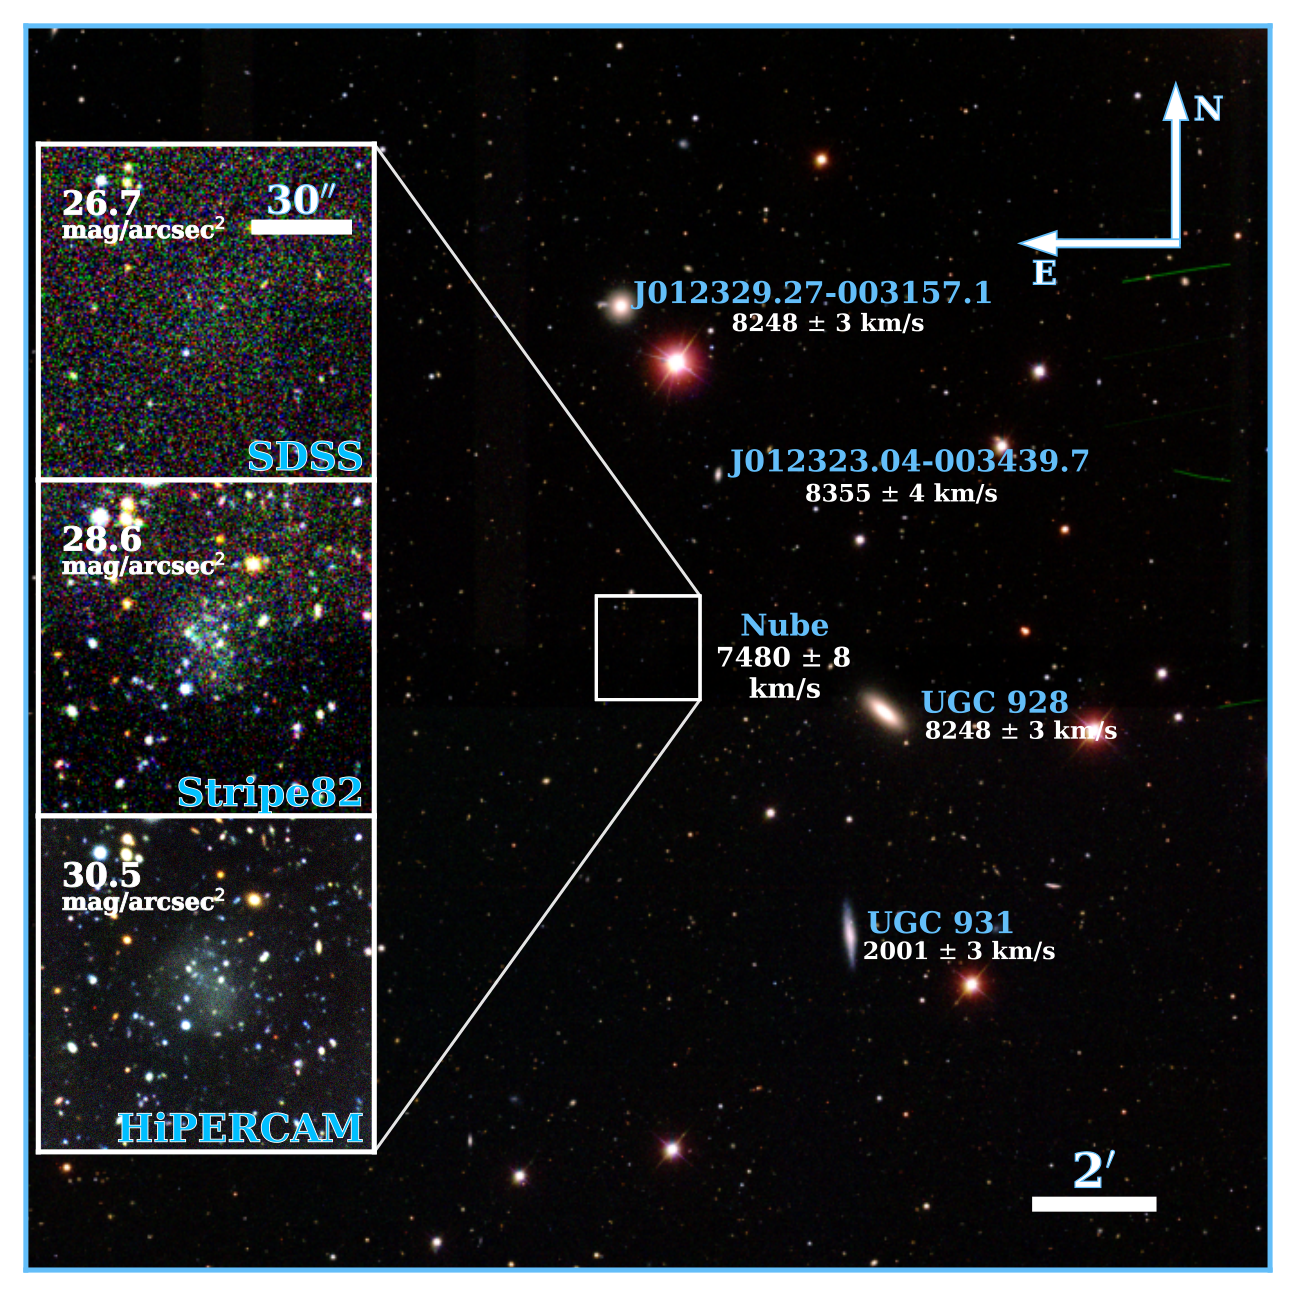
\includegraphics[width=0.82\textwidth]{nube_discovery.png}
\caption{The almost-dark galaxy Nube, adapted from the discovery paper \cite{montes2024nube} (arXiv source package). The main panel is the SDSS RGB image of the $20'\times20'$ field, in which the galaxy is invisible. The insets show the same object at $3\sigma$ $r$-band limiting depths of $26.7$, $28.6$, and $30.5$ mag\,arcsec$^{-2}$ over $10''\times10''$ boxes (SDSS, IAC Stripe 82, and HiPERCAM). An object with the stellar mass of the Small Magellanic Cloud emerges only in the deepest frame, which is the surface-brightness regime this mission reaches over wide contiguous areas (Section~\ref{sec:lsb}).}
\label{fig:nube}
\end{figure}

\begin{table}[tp]
\centering
\sffamily\small
\begin{tabularx}{\textwidth}{@{}p{3.2cm}p{6.4cm}X@{}}
\toprule
\textbf{System} & \textbf{Published properties} & \textbf{Place in the census}\\
\midrule
H\,\textsc{i}-bearing UDGs & 115 isolated, gas-rich, extremely diffuse field systems in high-spin dwarf halos with very low star-formation efficiency \cite{leisman2017} & Line-emitting gas-rich dwarfs, detected directly through H$\alpha$ and [O\,\textsc{iii}]\\
Coma\,P (HI1232$+$20) & Metal-poor H\,\textsc{i} cloud with $M_{\rm HI}/M_\star>200$ and only a trace very-low-surface-brightness stellar body \cite{janowiecki2015} & Almost-dark class, weak lines with an H\,\textsc{i} counterpart\\
Nube & Stellar mass of the Small Magellanic Cloud spread so thinly it evaded standard imaging, discussed as a possible fuzzy-dark-matter signature \cite{montes2024nube} & Almost-dark class, recovered by the deep-imaging stack (Figure~\ref{fig:nube})\\
VIRGOHI\,21 & Rotating H\,\textsc{i} structure with no optical counterpart, later discussed as a candidate tidal feature \cite{minchin2005,duc2008} & The false positive that isolation and dynamical-mass vetting removes\\
\bottomrule
\end{tabularx}
\caption{Benchmark systems along the almost-dark sequence and the class each occupies in the three-way classification of the census. The genuinely dark end of the sequence, gas halos with neither lines nor continuum, is the population the census is designed to isolate.}
\label{tab:darkbench}
\end{table}

\subsubsection{Environment as a Control: Field, Group, Cluster, and Void}

The sharpest current statement of the small-scale tension comes from the rotation curves of gas-rich field dwarfs and low-surface-brightness disks, for which homogeneous compilations such as the SPARC database of mass models provide spatially resolved inner kinematics for 175 galaxies \cite{lelli2016}. Figure~\ref{fig:sparcdiv} shows the diversity problem in the observed data. Two SPARC dwarfs of nearly the same outermost rotation speed, and hence comparable halo mass, whose inner curves differ by a factor of four in velocity. The interpretation of such comparisons is limited by the heterogeneity of existing samples, drawn from many surveys with different selection criteria, distance scales, and environments, so that intrinsic scatter is entangled with selection and systematic effects.

\begin{figure}[tp]
\centering
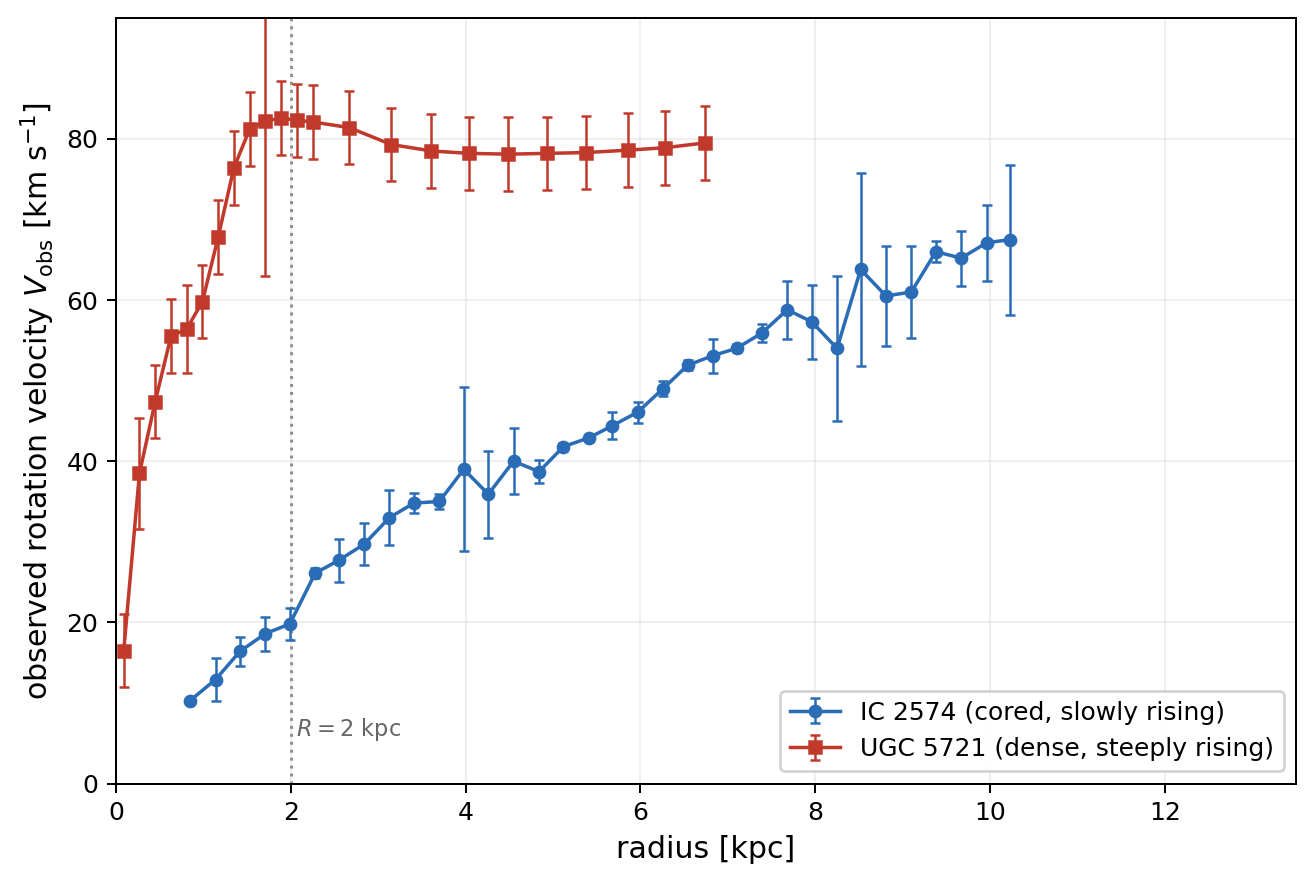
\includegraphics[width=0.72\textwidth]{sparc_diversity.png}
\caption{The rotation-curve diversity problem in the observed data, drawn directly from the public SPARC mass-model files \cite{lelli2016}. IC~2574 and UGC~5721 reach nearly the same outermost rotation speed, $67$ and $79$\,km\,s$^{-1}$. Hence, they occupy halos of comparable mass, yet at $2$\,kpc one rotates at $20$ and the other at $82$\,km\,s$^{-1}$, a factor of four in velocity and more than an order of magnitude in enclosed mass. Reproducing both extremes at fixed halo mass is the benchmark for the dark-matter models of Table~\ref{tab:dmmodels}. Self-interacting dark matter fits both galaxies with a single cross section \cite{kaplinghat2016,ren2019}.}
\label{fig:sparcdiv}
\end{figure}

Environment is what disentangles them. A dwarf in a cluster has been tidally stripped, ram-pressure swept, and harassed. A dwarf in a group has likely interacted with neighbors. Any inference about dark-sector inner structure from such systems must separate these environmental effects from the signal, because tidal stripping can lower a halo's central density in a way that superficially resembles a self-interaction core. A void dwarf has experienced essentially none of this, having assembled slowly and in isolation, and provides the zero-environment baseline against which field, group, and cluster populations can be compared at fixed halo mass. Differences that persist after the comparison are intrinsic, and those that vanish were environmental. The Void Galaxy Survey finds void dwarfs to be preferentially small, blue, gas-rich, late-type systems with extended undisturbed gas disks, consistent with slow, merger-free assembly in isolation \cite{kreckel2012}, more metal-poor at fixed stellar mass, and with a higher ratio of dark-matter halo mass to stellar mass than their denser-environment counterparts \cite{douglass2019}, exactly the signature expected if star formation is suppressed in shallow, isolated potentials \cite{hoeft2010}. Their extended, undisturbed disks are exactly the systems whose rotation curves most cleanly expose the core--cusp distinction and the diversity problem of Figure~\ref{fig:sparcdiv}, uncontaminated by the tidal confusion that limits cluster and group dwarfs. Because the mission observes void, field, group, and cluster dwarfs with the same instrument and selection function, it places all four environments on a common footing and measures the environmental dependence of both the galaxy--halo connection and the inner density structure, without the cross-survey systematics that have limited previous comparisons. This environmental span also sets the faint end of the galaxy--halo connection at the threshold of galaxy formation, where the relation between stellar and halo mass steepens and scatters. It tests whether a minimum halo mass for galaxy formation exists, and how sharply \cite{simon2019,bullock2017}. Present heterogeneous samples for this measurement are dominated by exactly the selection systematics that a single controlled survey removes.

\subsubsection{A Starlight-Independent Halo Census from Strong Lensing}

The deepest difficulty in counting low-mass halos through their galaxies is that one only ever counts the halos that lit up. Gravitational lensing removes this limitation by detecting halos through their mass alone, whether or not they contain stars. Gravitational imaging of extended Einstein rings has detected a dark satellite of mass $\sim2\times10^{8}\,M_\odot$ in a lens galaxy \cite{vegetti2012}, and high-resolution interferometry has localized a comparable subhalo in the lensed system SDP.81 \cite{hezaveh2016}. Flux-ratio and astrometric anomalies in multiply imaged quasars provide a complementary, statistical route to the same low-mass population. This is where the dwarf program and the strong-lens program of Section~\ref{sec:stronglens} reinforce each other. The strong-lens survey supplies the lens sample and the machine-learning modeling pipeline needed to detect substructure across a large sample, yielding a halo census from the dark side, while the wide-field dwarf and void survey yields the census from the luminous side with a controlled selection function and stellar-population diagnostics that say which halos formed stars and when. Agreement between the luminous and lensing halo mass functions would confirm that the faint-galaxy deficit is a star-formation effect within abundant cold-dark-matter halos, while a luminous deficit not matched by a lensing deficit would point to a genuine truncation of the mass function by warm or fuzzy dark matter. Neither probe alone is decisive, but together they are, and the mission delivers both.

\subsubsection{Detection Strategy: Slitless Spectroscopy, Imaging, and H\,\textsc{i} Cross-Match}

A slitless survey at $R=1000$ cannot resolve the few-km\,s$^{-1}$ internal velocity dispersions of dwarfs, which lie a factor of thirty below its resolution element and remain the province of high-resolution multi-object spectroscopy. The mission's contribution is the discovery and characterization that gate the small-scale dark-matter tests, and it does so by inverting the usual selection. Continuum-selected imaging surveys, even deep ones, miss gas-rich star-poor systems precisely because their stellar continuum is faint, which is why most dark-galaxy candidates have been found in blind H\,\textsc{i} surveys rather than optically. A blind slitless spectroscopic survey instead detects galaxies by their emission lines, H$\alpha$, [O\,\textsc{iii}], and [O\,\textsc{ii}], independently of continuum brightness, so it is intrinsically sensitive to objects with high line-to-continuum ratios. A modest amount of ongoing star formation in an otherwise optically dark halo produces detectable line emission against a negligible continuum, the easiest possible target for grism spectroscopy. Figure~\ref{fig:darkgal} gives the exposure to a $5\sigma$ H$\alpha$ detection as a function of star-formation rate for a galaxy in a nearby void at $z=0.05$, using the standard Kennicutt calibration ${\rm SFR}\simeq7.9\times10^{-42}\,(L_{\rm H\alpha}/{\rm erg\,s^{-1}})\,M_\odot\,{\rm yr^{-1}}$ \cite{kennicutt1998}. The survey reaches $\sim3\times10^{-3}\,M_\odot\,{\rm yr}^{-1}$ in about an hour and $\sim10^{-3}\,M_\odot\,{\rm yr}^{-1}$ in a deep pointing, deep into the regime of the faintest known gas-rich dwarfs. This floor is again the idealised slitless-calculator line-flux depth rather than a survey-anchored one, so it carries the same optimistic margin quantified in Section~\ref{sec:etc}.

Cross-matching these emission-line detections against H\,\textsc{i} maps from current and future radio surveys (ALFALFA, Apertif, MeerKAT, and ultimately the SKA) completes the gas-plus-stars accounting, delivering a three-way classification. Systems seen in both lines and H\,\textsc{i} are gas-rich star-forming dwarfs. Systems seen in H\,\textsc{i} with only faint line emission are the almost-dark population. Systems seen in H\,\textsc{i} with no line emission and no continuum are the candidate genuinely dark halos that the void phenomenon predicts. A credible claim for the last class must combine several discriminants rather than rely on an H\,\textsc{i} detection alone. Isolation deep in a void, far from any plausible parent, is the first, since a candidate there cannot easily be tidal debris. A dynamical mass budget far exceeding the gas-plus-stars mass is the second, since tidal debris is baryon-dominated. A deep optical non-detection is the third, where the mission's stable, airglow-free imaging sets the most stringent surface-brightness limits, individually and by stacking. This combination is what converts a heterogeneous list of curiosities into a quantitative measurement of how galaxy formation fails at the lowest halo masses.

The void search is built around a set of nearby voids selected from catalogs constructed from the SDSS and DESI redshift surveys \cite{sutter2012}, restricted to $z\lesssim0.05$ to keep the diagnostic nebular lines within the most sensitive part of the band and to spatially resolve even very low-mass dwarfs. Tiling the interiors of a sample of large voids to the wide- and medium-tier depths yields a volume-complete emission-line census whose faint end measures the void galaxy luminosity and star-formation-rate functions with a uniform, space-based selection that heterogeneous, atmosphere-limited ground-based void surveys cannot match. Because the search exploits the same emission-line sensitivity, multi-roll depth, and wide field that the flagship survey already delivers, the void, field, group, and cluster volumes are all covered at marginal additional cost. Table~\ref{tab:dwarfvoidreach} summarizes the resulting reach. Figure~\ref{fig:voidwedge} of Section~\ref{sec:voidphenom} makes the underlying target selection concrete with real archival data.

\begin{figure}[tp]
\centering

\includegraphics[width=0.55\textwidth]{darkgal_exptime_vs_sfr.png}
\caption{Exposure to a $5\sigma$ H$\alpha$ detection versus star-formation rate for a void galaxy at $z=0.05$, from the Kennicutt SFR calibration. The $1$ and $12$\,hr levels are marked.}
\label{fig:darkgal}
\end{figure}

\begin{table}[tp]
\centering
\sffamily\small
\begin{tabularx}{\textwidth}{@{}p{3.4cm}p{3.6cm}X@{}}
\toprule
\textbf{Target class} & \textbf{Selection} & \textbf{Dark-matter use}\\
\midrule
Dwarf/UDG census (field, group, cluster) & Deep imaging $+$ grism, wide field & Halo mass function and abundance versus CDM, WDM, and FDM suppression; membership, distances, and stellar populations from emission/absorption redshifts, SBF, and TRGB\\
Structural diversity & Sizes, central surface brightness, across environments & Distribution of inner densities (SIDM core/collapse, FDM solitons) and the environmental control of Section~\ref{sec:dwarfvoid}\\
Star-forming void dwarfs & Blind emission lines (H$\alpha$, [O\,\textsc{iii}]) & Faint end of the void luminosity function and low-mass halo abundance versus WDM and FDM\\
Almost-dark / H\,\textsc{i}-bearing UDGs & Lines $+$ H\,\textsc{i} cross-match & High gas-to-star systems and the star-formation threshold in low-mass halos\\
Optically dark halos & H\,\textsc{i} detection, no line emission & Census of star-free gas halos, the void phenomenon\\
\bottomrule
\end{tabularx}
\caption{Planning reach of the combined dwarf and void dark-matter program. The mission delivers wide-field discovery, membership, and stellar-population characterization with a uniform selection function across environments. Internal stellar velocity dispersions are below the $R=1000$ resolution and require high-resolution follow-up, while lensing substructure (Section~\ref{sec:stronglens}) provides a starlight-independent halo census.}
\label{tab:dwarfvoidreach}
\end{table}

\subsubsection{Program Scope}

The program is scoped as a wide-field census plus spectroscopic characterization across field, group, cluster, and void environments, combining the wide-survey imaging and grism data with deeper targeted fields around selected nearby hosts and groups and a dedicated volume-complete search of nearby void interiors combined with archival and forthcoming H\,\textsc{i} coverage. It is deliberately structured as a multi-probe attack on a single question, the particle nature of dark matter, rather than a collection of unrelated measurements. The abundance and radial distribution of dwarfs across environments test the halo mass function and its small-scale cutoff, sharpest in the void interiors where it is least contaminated by accretion and tides. The structural and chemical diagnostics separate baryon-driven from dark-sector core formation. The strong-lens substructure census counts halos independently of their starlight. The void, field, group, and cluster sub-samples, observed with a single selection function, control the environmental systematics that have confounded previous comparisons. Each probe alone is suggestive and degenerate. The value lies in their combination over one homogeneous catalog, confronted with the predicted distributions from the team's high-resolution self-interacting and wave dark-matter simulations. Because the census rides the survey data taken for the flagship program, its dark-matter return is a by-product of already-scheduled observations. The concrete deliverables are the following.
\begin{itemize}[leftmargin=1.4em,itemsep=1pt,topsep=2pt]
\item A uniform dwarf and ultra-diffuse-galaxy catalog with structural parameters, stellar metallicities, ages, and a controlled selection function across field, group, host, and void environments.
\item The faint-end galaxy stellar-mass function, satellite radial distributions, and void galaxy and H\,\textsc{i} mass functions that jointly constrain the halo mass function and its warm or fuzzy cutoff.
\item The joint distribution of central density, stellar mass, star-formation history, and environment that separates baryon-driven from SIDM and FDM core formation.
\item A catalog of almost-dark and H\,\textsc{i}-bearing ultra-diffuse systems, and a prioritized target list of central-density, metallicity, and isolation/dynamics-vetted dark-halo-candidate outliers for high-resolution kinematic and deep H\,\textsc{i} follow-up with the SKA and its precursors.
\item A starlight-independent halo census from the strong-lens substructure program of Section~\ref{sec:stronglens}, confronted against the luminous census within the same dark-matter models.
\item Improved interior tracer densities for void-dynamics cosmology, as a by-product of the same redshift survey.
\end{itemize}

\clearpage
\section{Program Triage}

Table~\ref{tab:triage} collects the program-level scope implied by the preceding sections. It separates the core ELG BAO/RSD survey from companion programs whose requirements are compatible with the same survey architecture, spectroscopic or imaging, but should not drive the flagship performance claims.

\begin{table}[tp]
\centering
\sffamily\footnotesize
\setlength{\tabcolsep}{3.5pt}
\renewcommand{\arraystretch}{0.94}
\begin{tabularx}{\textwidth}{@{}p{2.1cm}p{1.6cm}p{2.7cm}p{2.9cm}p{2.9cm}Y@{}}
\toprule
\textbf{Program} & \textbf{Priority} & \textbf{Observing mode} & \textbf{Area/sample} & \textbf{Depth/exposure} & \textbf{Decision}\\
 & & imaging, spectroscopy, or both & area in deg$^2$ or object count & flux in erg s$^{-1}$ cm$^{-2}$; time in hr & \\
\midrule
ELG BAO/RSD & Flagship & Concurrent imaging $+$ 3-roll slitless & 100--300 \degti; $10^6$--$3\times10^6$ redshifts & $F_{5\sigma}=10^{-16}$ wide; $2.5\times10^{-17}$ deep & \textcolor{green}{Core mission}\\
SN Ia & Major companion & Dedicated cadenced field inside the wide tier (LSST-DDF-style) $+$ targeted slitless typing & 5--10 \degti time-domain field nested in the wide tier; 1000--3000 discoveries & 2--30 hr spectra; useful typing to $z\simeq1.5$ & \textcolor{green}{Proceed}\\
LSB blind census & Survey by-product & Imaging only (rides flagship tiers) & 100--300 \degti; $\gtrsim$500--1400 LSBGs/UDGs at the published DES density alone & $\mu_{5\sigma}(10'',g)=29.8$--$31.3$; concurrent survey imaging, no extra time & \textcolor{green}{Proceed}\\
LSB ultra-deep fields & Major companion & Imaging only & two $2.25$ \degti\ low-cirrus fields & 16 hr per tile in simultaneous $g$+$H$; $\mu_{5\sigma}(10'')=31.5/31.2$ & \textcolor{green}{Proceed}\\
Imaging wide extension & Major companion & Imaging only & $+612$ \degti\ imaging-only; Lockman-Hole N and south-polar S fields & $0.25$ hr per tile in simultaneous $g$+$H$; $\mu_{5\sigma}(10'',g)=29.2$ & \textcolor{green}{Proceed}\\
ICL targeted clusters & Major companion & Imaging only (targeted deep stacks) & 20--40 clusters at $0.02\lesssim z\lesssim0.10$ & multi-roll 4--64 hr per cluster; $\mu_{5\sigma}(10'')\simeq30.4$--$31.9$ & \textcolor{green}{Proceed}\\
High-$z$ quasars & Major companion & Targeted slitless spectroscopy & 50--100 quasars at $z>6.5$ & $3\times2$--$3\times5$ hr per target & \textcolor{green}{Proceed}\\
Ly$\alpha$ forest & Calibration & Targeted slitless spectroscopy & 3000--5000 quasars at $2.1<z<3.5$ & 1--6 hr; $m_{\rm AB}\lesssim22.5$ & \textcolor{gold}{Moderate claims}\\
Strong lenses & Pathfinder & Imaging (finding) $+$ targeted slitless spectroscopy & 20--30 clean systems & $3\times2$--$3\times4$ hr plus IFU support & \textcolor{gold}{Ancillary}\\
LBG topology & Ancillary & Targeted slitless spectroscopy & 100--200 bright systems in overdensities & $3\times5$--$3\times10$ hr & \textcolor{rose}{Do not flagship}\\
\bottomrule
\end{tabularx}
\caption{Program-level numerical scope. Exposure entries quote science exposure and explicitly include the required three slitless orientations, but not operational overhead. The observing-mode column does not count serendipitous SN discoveries that other imaging tiers' repeat visits might incidentally yield, since that channel's rate is not forecast here.}
\label{tab:triage}
\end{table}

\clearpage
\section{Observing Architecture}

\begin{figure}[tp]
\centering
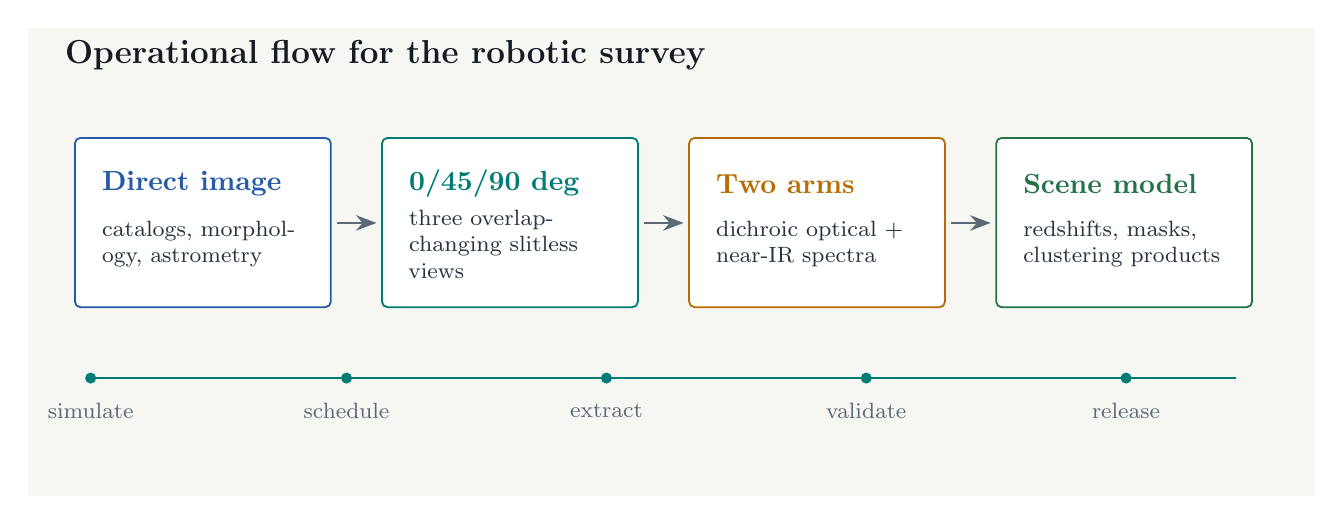
\begin{tikzpicture}[font=\sffamily]
  \fill[paper] (-0.35,-0.25) rectangle (16.0,5.7);
  \node[anchor=west,font=\bfseries\large,color=ink] at (0,5.35) {Operational flow for the robotic survey};
  \foreach \x/\title/\body/\col in {
    0.25/{Direct image}/{catalogs, morphology, astrometry}/blue,
    4.15/{0/45/90 deg}/{three overlap-changing slitless views}/teal,
    8.05/{Two arms}/{dichroic optical + near-IR spectra}/gold,
    11.95/{Scene model}/{redshifts, masks, clustering products}/green} {
    \fill[white,draw=\col,rounded corners=2pt,line width=0.65pt] (\x,2.15) rectangle ++(3.25,2.15);
    \node[anchor=west,font=\bfseries,color=\col] at (\x+0.22,3.72) {\title};
    \node[anchor=west,text width=2.75cm,color=softink,font=\footnotesize] at (\x+0.22,2.95) {\body};
  }
  \foreach \xa/\xb in {3.58/4.08,7.48/7.98,11.38/11.88}
    \draw[-{Stealth[length=2.6mm]},line width=0.8pt,color=muted] (\xa,3.22) -- (\xb,3.22);
  \draw[teal,line width=0.9pt] (0.45,1.25) -- (15.0,1.25);
  \foreach \x/\lab in {0.45/{simulate},3.7/{schedule},7.0/{extract},10.3/{validate},13.6/{release}}
    {
    \fill[teal] (\x,1.25) circle (2pt);
    \node[anchor=north,color=muted,font=\footnotesize] at (\x,1.05) {\lab};
    }
\end{tikzpicture}
\caption{The robotic concept is treated as a data-production system. Direct imaging, slitless spectroscopy, roll diversity, and scene modeling are inseparable.}
\label{fig:ops}
\end{figure}

\subsection{Wide Survey Mode}

The wide survey uses the \fovlarge\ field, two band-limited grism settings per wavelength channel, and three orientations. The practical unit of observation is therefore a bundle that contains direct imaging, grism exposures at the three roll angles of $0^\circ$, $45^\circ$, and $90^\circ$, dithers, and calibration overhead. Every survey time estimate in this document quotes all of these components rather than a single ``exposure per pointing''.

Table~\ref{tab:timeline} gives the resulting observing-program envelope. The year ranges are not a fixed schedule but an existence proof, showing that commissioning, the reference fields, the wide ELG map, the calibration tiers, and the companion programs fit together within a multi-year robotic survey.

\begin{table}[tp]
\centering
\sffamily\small
\begin{tabularx}{\textwidth}{@{}p{3.0cm}p{3.0cm}p{3.2cm}Y@{}}
\toprule
\textbf{Mission phase} & \textbf{Nominal period} & \textbf{Science time} & \textbf{Main deliverable}\\
 & mission year & hr & \\
\midrule
Commissioning and reference fields & Year 1 & 300--500 hr & Wavelength solution, PSF/trace model, 0/45/90 deblending validation, ultra-deep reference fields.\\
Wide ELG BAO/RSD & Years 1--4 & 1200--2500 hr & 100--300 \degti ELG redshift map with survey masks and random catalogs.\\
Medium/deep ELG tiers & Years 2--5 & 600--1200 hr & Completeness, purity, luminosity-function, and overlap-calibration transfer functions.\\
Imaging-only wide extension & Years 2--5 & $\sim$610 hr & LSBG/UDG census beyond the spectroscopic footprint, $\sim$306 \degti/cap in $g$+$H$.\\
Ultra-deep imaging fields & Years 2--5 & $\sim$290 hr & Nube-depth ($\mu_{5\sigma}\sim31.5$ $g$, $31.2$ $H$) LSBG/UDG imaging in two dedicated fields.\\
SN Ia time-domain field & Years 2--5 & 800--1600 hr & Spectral time series and host-scene models for $z\lesssim1.5$ SNe Ia, from a cadenced field nested inside the wide tier.\\
Quasar and reionization targets & Years 2--5 & 600--1200 hr & Ly$\alpha$ calibration spectra and $z>6.5$ damping-wing sample.\\
Pathfinders and contingency & Years 3--5 & 300--700 hr & Strong-lens, LBG, ICL cluster imaging, and special-field programs.\\
\bottomrule
\end{tabularx}
\caption{Illustrative observing program. The range reflects field-of-view choice, number of filters per channel, overhead model, and final survey area. Of the four tasks bundled into the Year~1 commissioning line, the 0/45/90 deblending validation (Section~\ref{sec:e2eval}) is the least mature and the highest-risk. The quoted hours are not yet apportioned between it and the other three.}
\label{tab:timeline}
\end{table}



The wide survey targets two high-Galactic-latitude caps that avoid the Milky Way and overlap the existing wide surveys, chosen together with the legacy deep fields they enclose as described in Section~\ref{sec:deepfields}.

\subsection{Deep and Time-Domain Mode}

The \fovsmall\ mode is valuable for deeper fields where the science is not area-limited, such as supernova cadence fields, the targeted intracluster-light cluster program of Section~\ref{sec:lsb}, deep calibration fields, quasar monitoring, and algorithm-validation fields with existing spectroscopy. It should not define the wide RSD survey unless the mission accepts a much smaller cosmological footprint.

\clearpage
\section{Flat Fielding and the Cirrus Foreground in the Imaging Surveys}\label{sec:flatcirrus}

Deep surface photometry is a mission-wide concern rather than a property of any single program. The same two systematic terms govern the direct imaging of the wide ELG tiers, the imaging-only wide extensions, the two ultra-deep fields, and the targeted cluster program of Section~\ref{sec:lsb}. Therefore, the control strategy is collected here once with the ultra-deep fields as the most demanding case.

Surface photometry at $\mu\gtrsim29$ mag\,arcsec$^{-2}$ is limited by two instrumental-and-foreground terms that must be controlled together, the multiplicative flat field and the additive diffuse foregrounds. The flat-field requirement is severe because the science signal sits so far below the sky. A residual illumination error of one percent on the $\mu_g\simeq22$ mag\,arcsec$^{-2}$ zodiacal background imprints a false diffuse signal at $\mu_g\simeq27$, more than four magnitudes above the ultra-deep limit of $31.5$. Hence, the low-order flat must be controlled to the $10^{-4}$ level over the field.

The techniques that reach this level are established across the deep surveys. They share one principle, that the trusted low-order reference is the sky and the stars rather than any internal lamp, because a lamp or dome screen illuminates the optics differently from the sky and imprints its own scattered-light pattern. The oldest of these methods is the star flat, in which repeated photometry of the same stars stepped across the focal plane solves directly for the position-dependent photometric response \cite{manfroid1996}. It remains the working correction of a modern wide-field mosaic, since the Dark Energy Camera detrending applies exactly such star-flat solutions on top of its dome flats, using the internal consistency of on-sky observations to separate quantum efficiency, pixel-size variation, and stray light \cite{bernstein2017pasp}. The SDSS generalised the idea to the survey scale as photometric self-calibration (\"ubercalibration), a single least-squares solution over all overlapping scans that reached one-percent relative calibration in $griz$ over $8500$\,deg$^2$ \cite{padmanabhan2008}. Survey-design simulations show that what makes such a solution converge is precisely the strategy of returning the same sources to very different focal-plane positions \cite{holmes2012}. For the diffuse regime itself the working reference is the dark night sky. The deepest wide-aperture ground photometry to date, $\mu_r=31.5$ mag\,arcsec$^{-2}$ ($3\sigma$, $10\times10$\,arcsec$^2$) at the 10.4-m GTC, was flattened with dark-sky flats built from the dithered science exposures themselves \cite{trujillofliri2016}. At the hardware end, tunable monochromatic illumination measured against calibrated photodiodes transfers a laboratory throughput standard to the full telescope-plus-detector system, the route proposed for percent-level ground-based photometry \cite{stubbs2006}.

The adopted strategy combines these methods on the space platform, using the sky itself as the flat source. Lamp-style internal flats calibrate only the high-frequency pixel response. The low-order illumination is measured from the science data as a dark-sky superflat, the median of the many dithered exposures of the survey with all sources masked, which works in space because the zodiacal light is smooth on the field scale and does not fluctuate with time the way airglow does. The large-amplitude dithers and the three roll angles of the survey separate detector-fixed patterns from sky-fixed signal by construction, the same redundancy the slitless deblending already requires. The overlap of neighbouring tiles admits the joint least-squares solution for the multiplicative flat and the additive sky that the \"ubercalibration introduced \cite{padmanabhan2008}. The stability of a space platform is what makes this converge, since the same star field revisited at different rolls and offsets ties every pixel to a common photometric zero point.

The Galactic cirrus enters differently, as a real additive foreground rather than a calibration error. As anticipated, it is not negligible even in the cleanest fields. At the field-mean $857$\,GHz intensities of the chosen ultra-deep fields the scattered-light scaling of Section~\ref{sec:etc} predicts diffuse galactic light at $\mu_g\simeq27.2$ mag\,arcsec$^{-2}$ using the measured optical $b(\lambda)$ ratios \cite{ienaka2013}, extrapolated to $\mu_H\simeq26.7$ mag\,arcsec$^{-2}$ in the near-infrared, several magnitudes brighter than the depth limit. Therefore, it is the \emph{structure} of the cirrus rather than its mean level that sets the true confusion floor for the diffuse science. Figure~\ref{fig:cirrusfil} shows that structure directly, the same cirrus filament imaged by \emph{Herschel} at $250\,\mu$m and in deep optical data, where the dust appears at higher signal-to-noise than in the far-infrared map that conventionally traces it \cite{roman2020}. Three controls are applied. First, the field choice itself is the strongest lever, because the cirrus fluctuation power scales roughly as the cube of the mean brightness \cite{gautier1992}. Hence, observing at a quarter of the median sky brightness suppresses the fluctuation power by a factor of order fifty relative to typical high-latitude sky. Second, the Planck $857$\,GHz and IRAS $100\,\mu$m maps provide an external template of the structured cirrus, scaled to the optical and near-infrared through the measured $b(\lambda)$ ratios \cite{ienaka2013}, which subtracts the large-scale component and flags the residual regions where diffuse detections should be distrusted. Third, colour discriminates the survivors, since the scattered-light spectrum of the cirrus differs from galaxy light, the measured cirrus colours sitting bluer in $r-i$ at a given $g-r$ than any stellar population (Figure~\ref{fig:cirruscolors}) \cite{roman2020}. Cirrus knots masquerading as LSBGs are a known contaminant that ground-based LSB catalogs must vet against \cite{zaritsky2023}, a vetting the five-band photometry performs object by object.

\begin{figure}[tp]
\centering
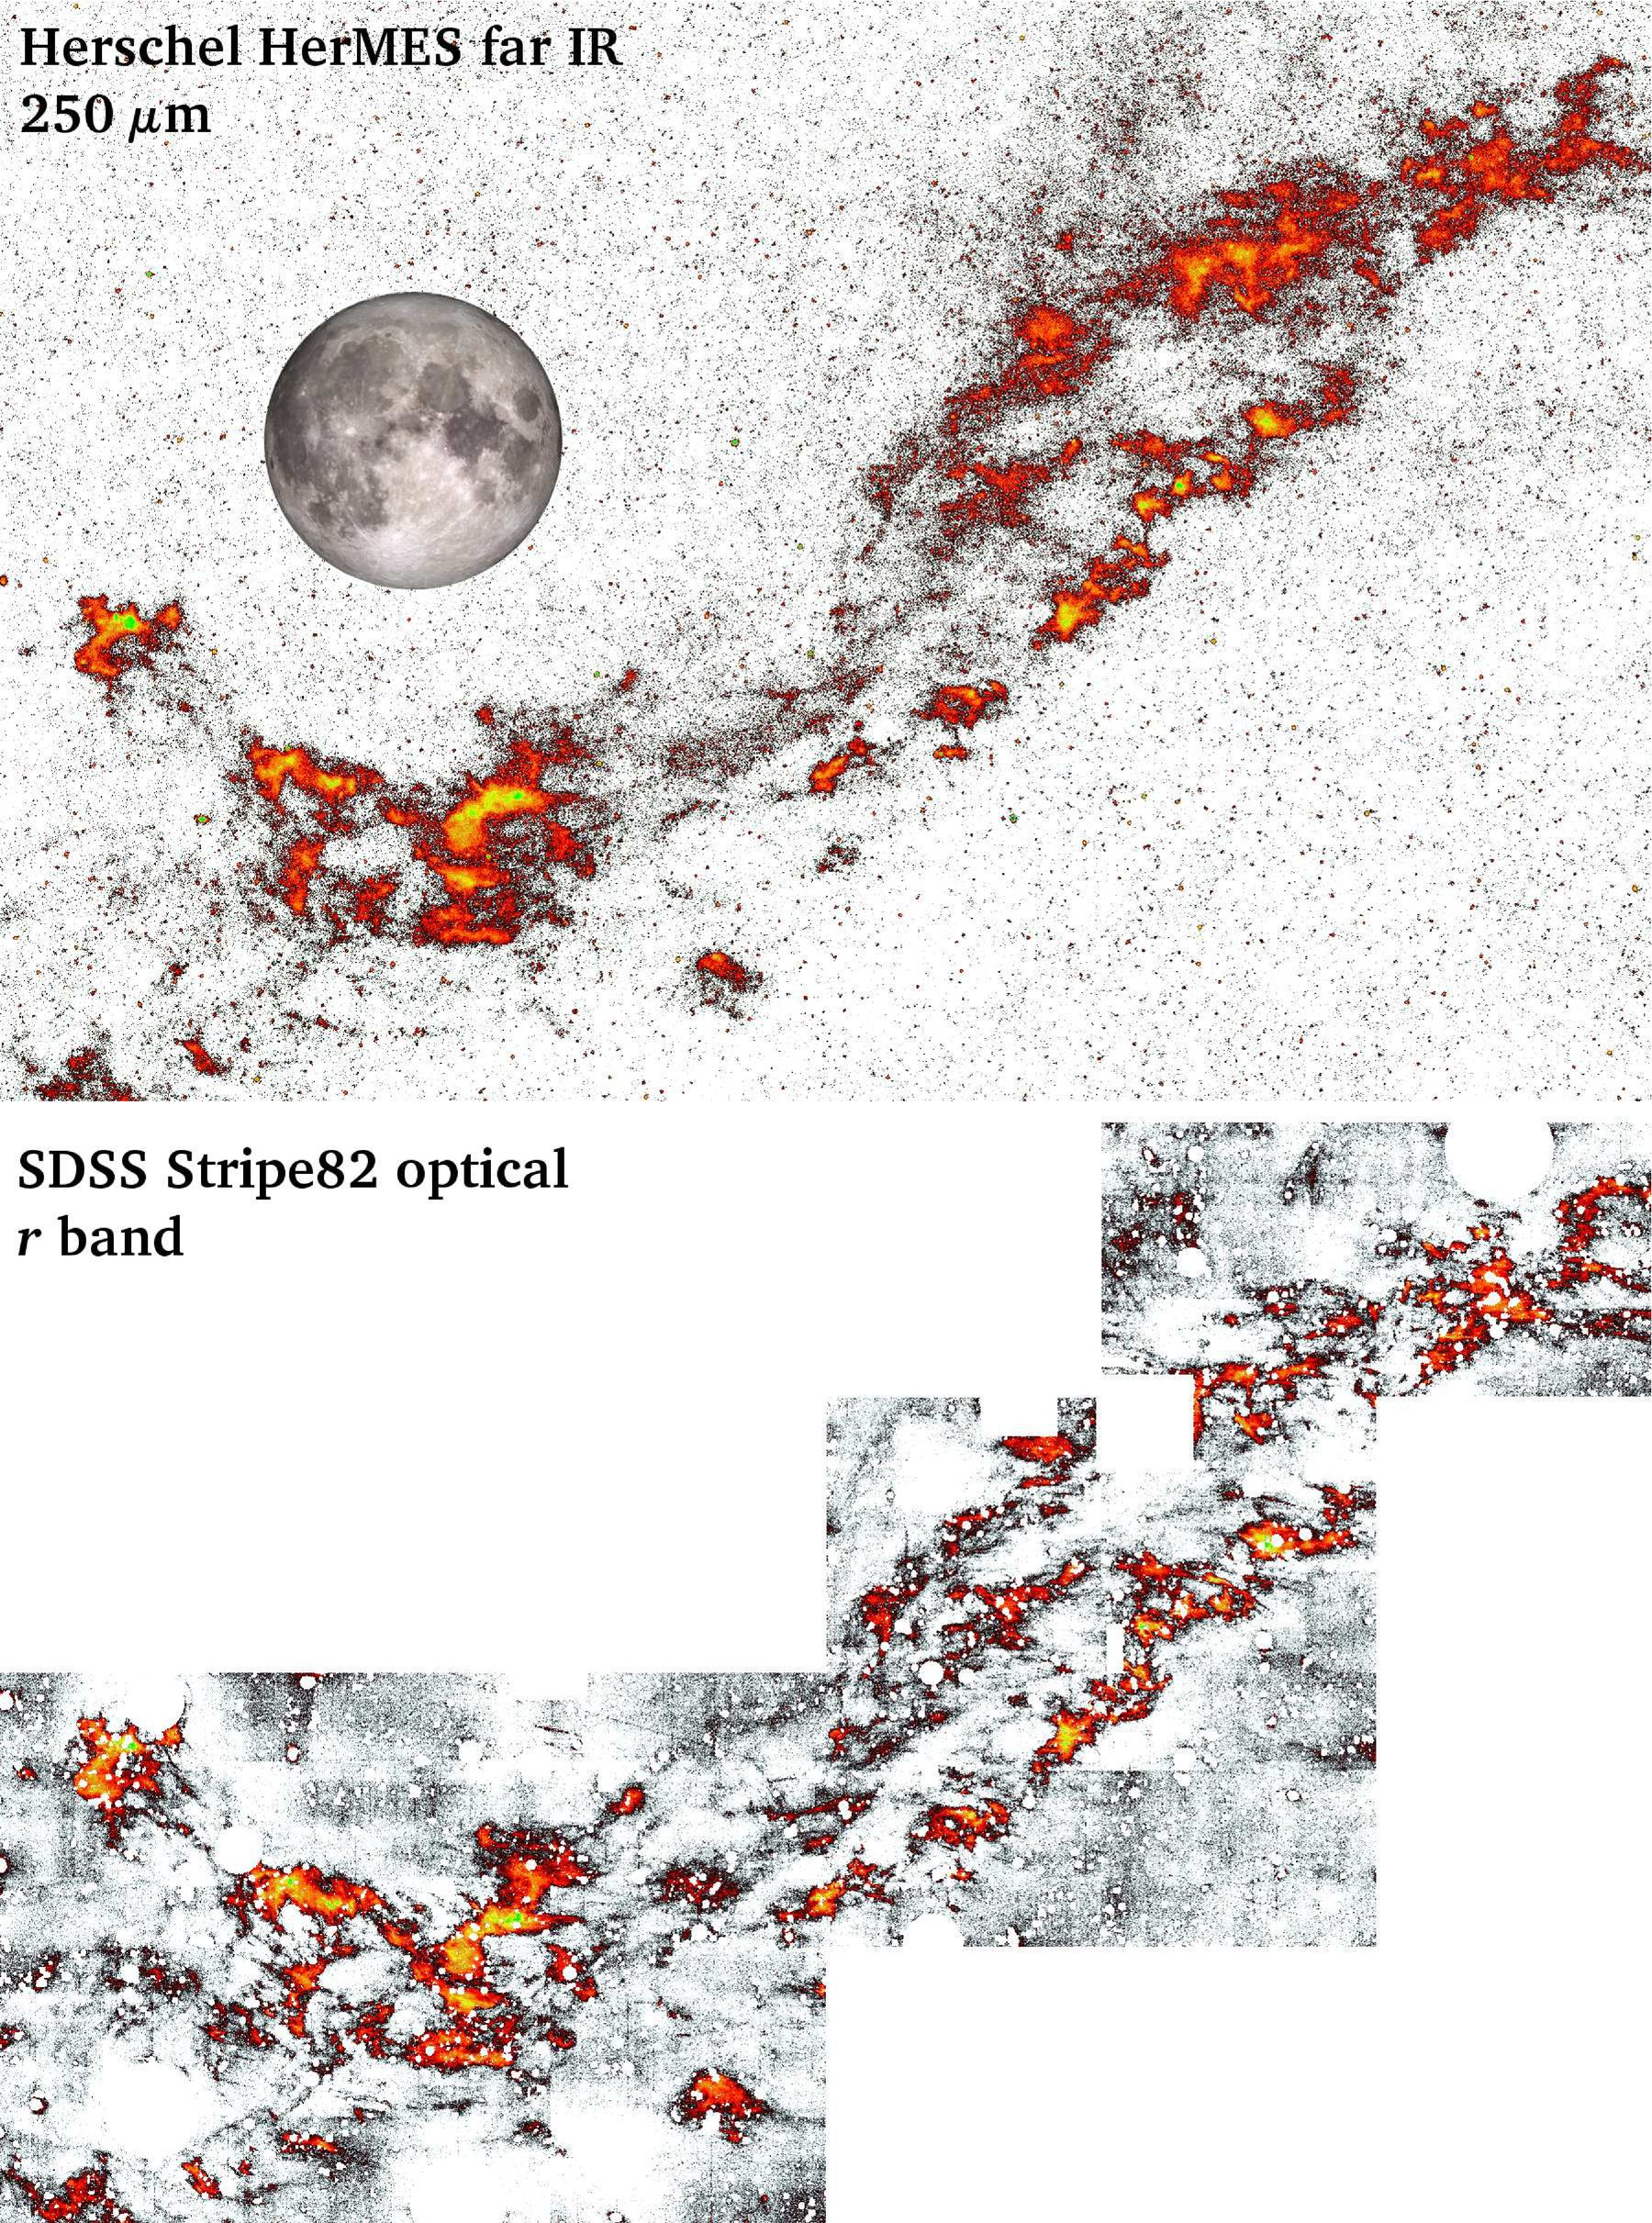
\includegraphics[width=0.6\textwidth]{cirrus_optical_ir.jpg}
\caption{The same Galactic cirrus imaged in the far infrared and in deep optical data, the \emph{Herschel}/SPIRE $250\,\mu$m map (top) and the deep SDSS Stripe82 $r$-band mosaic (bottom) with the full Moon placed for angular scale. The deep optical imaging detects the cirrus at higher signal-to-noise than the far-infrared map that is conventionally used to trace it, which is why the structured cirrus, rather than its smooth mean level, sets the confusion floor for diffuse science at the depths of this proposal and why the infrared template must be supplemented by controls in the survey's own bands. [courtesy: Rom\'an, Trujillo \& Montes 2020 \cite{roman2020}]}
\label{fig:cirrusfil}
\end{figure}

\begin{figure}[tp]
\centering
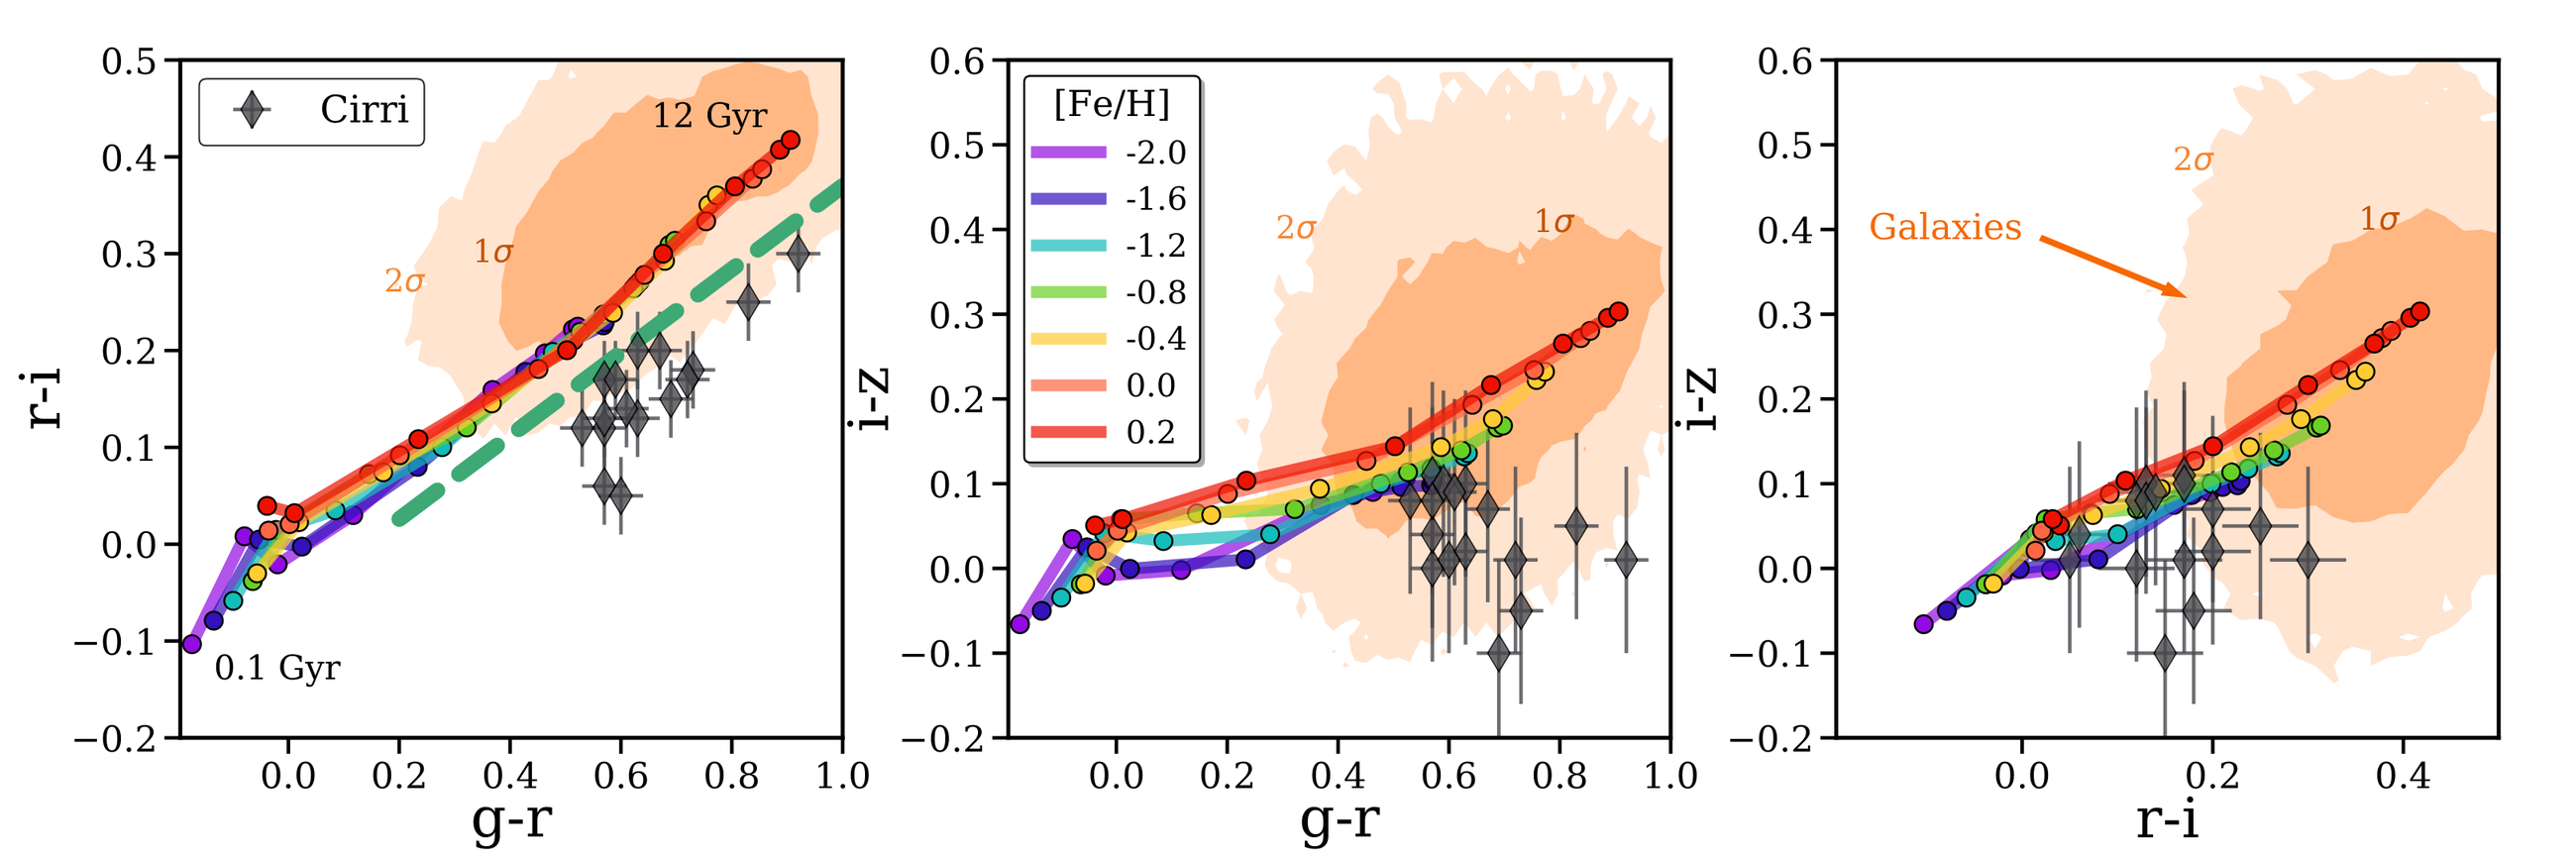
\includegraphics[width=\textwidth]{cirrus_colors.png}
\caption{Optical colour separation of Galactic cirrus from extragalactic light. The grey diamonds are the measured colours of cirrus fields in the deep SDSS Stripe82 data, the orange contours enclose $68\%$ and $95\%$ of the pixels of real galaxies, and the coloured tracks are single-stellar-population models spanning age and metallicity. The cirrus sits bluer in $r-i$ at a given $g-r$ than any stellar population, with the dashed line in the left panel separating the dust regime from the extragalactic one. This is the object-by-object vetting that the five-band survey photometry applies to every diffuse detection. [courtesy: Rom\'an, Trujillo \& Montes 2020 \cite{roman2020}]}
\label{fig:cirruscolors}
\end{figure}

\clearpage
\section{Expected Deliverables}

The mission will release science-ready products rather than only calibrated images:
\begin{itemize}
  \item direct-image source catalogs with morphology parameters and astrometric covariance;
  \item calibrated 2D slitless exposures for each filter, roll, and dispersion direction;
  \item extracted 1D spectra with contamination models and covariance;
  \item probabilistic redshift catalogs with line-identification likelihoods;
  \item survey masks, random catalogs, and completeness maps for clustering analyses;
  \item supernova host-scene models and binned spectral time series;
  \item high-redshift quasar continuum fits and damping-wing likelihood products;
  \item public image-level simulations matching the final survey selection.
\end{itemize}

\clearpage
\section{Conclusion}

The \facility\ is a coherent cosmology mission when it is built around the real strength of slitless spectroscopy. That strength is dense, homogeneous, robotic redshift mapping over large solid angle. The \fovlarge\ option is therefore not an optional upgrade but the enabling survey mode for the ELG BAO/RSD program. The \fovsmall\ mode remains useful for deep calibration, supernova cadence, and targeted quasar work. The supernova program has a quantified reach of its own, since the rest-frame $U$ and NUV magnitudes that separate the optical twins are measured at subgroup precision to $z\simeq0.9$--$1.1$ in the standard two-hour visits and to $z\simeq1.3$--$1.5$ in ten-hour stacks (Figure~\ref{fig:snuvlimit}), covering the redshift range that anchors the dark-energy measurement. The deep imaging that rides the spectroscopic tiers has a matching one, since it uses emission-line redshifts to recover the low-surface-brightness galaxies that the team's Horizon Run 5 mock surveys show are missing from the observed stellar mass function at $0.625\le z\le2$ (Figure~\ref{fig:hr5gsmf}). Therefore, the census turns the faint end of that function from a selection-truncated calibration target into a direct test of stellar feedback. The dwarf-galaxy and void program has a matching reach of its own, since the same uniform selection function followed from field to void to cluster environment lets the halo mass function and the inner density structure of dark-matter halos be tested against cold, self-interacting, and fuzzy dark matter without the cross-survey systematics that limited previous comparisons.

Read as a single physics question rather than a list of programs, the mission's most distinctive claim is this. Roman, Euclid, DESI, and Rubin will each map far larger volumes and much larger samples than this concept, and nothing above claims otherwise. None of them is built around one uniformly selected, matched-depth sample spanning field, group, cluster, and void environments with the same instrument and selection function. That comparison, not sample size, is what separates a genuine self-interacting or wave-dark-matter signal in the inner structure of the lowest-mass halos from an environmental or selection systematic, the confound that has limited every previous comparison assembled from heterogeneous surveys (Section~\ref{sec:dwarfvoid}). Whether dark matter is cold and collisionless, self-interacting, or wave-like at the smallest resolved scales is the one question this mission is positioned to answer in a way the larger, wider missions are not, precisely because it is not trying to be larger or wider.

The revised mission statement is:
\begin{leadbox}[title=Mission Statement]{teal}
\textbf{The \facility\ will conduct a band-limited, multi-roll, $R=1000$ slitless spectroscopic survey optimized for ELG BAO/RSD cosmology, supported by supernova and high-redshift quasar programs that exploit the stability and multiplexing of space-based robotic operations, and by a low-surface-brightness and dwarf-galaxy program that tests the particle nature of dark matter.}
\end{leadbox}

Figure~\ref{fig:surveytimeline} draws all of the above together into one Sun-angle-weighted rendering of Table~\ref{tab:timeline}'s observing-program envelope, an illustrative check that the whole set of programs fits within the field-of-regard of a real orbit rather than only within an hours budget.

\begin{figure}[tp]
\centering
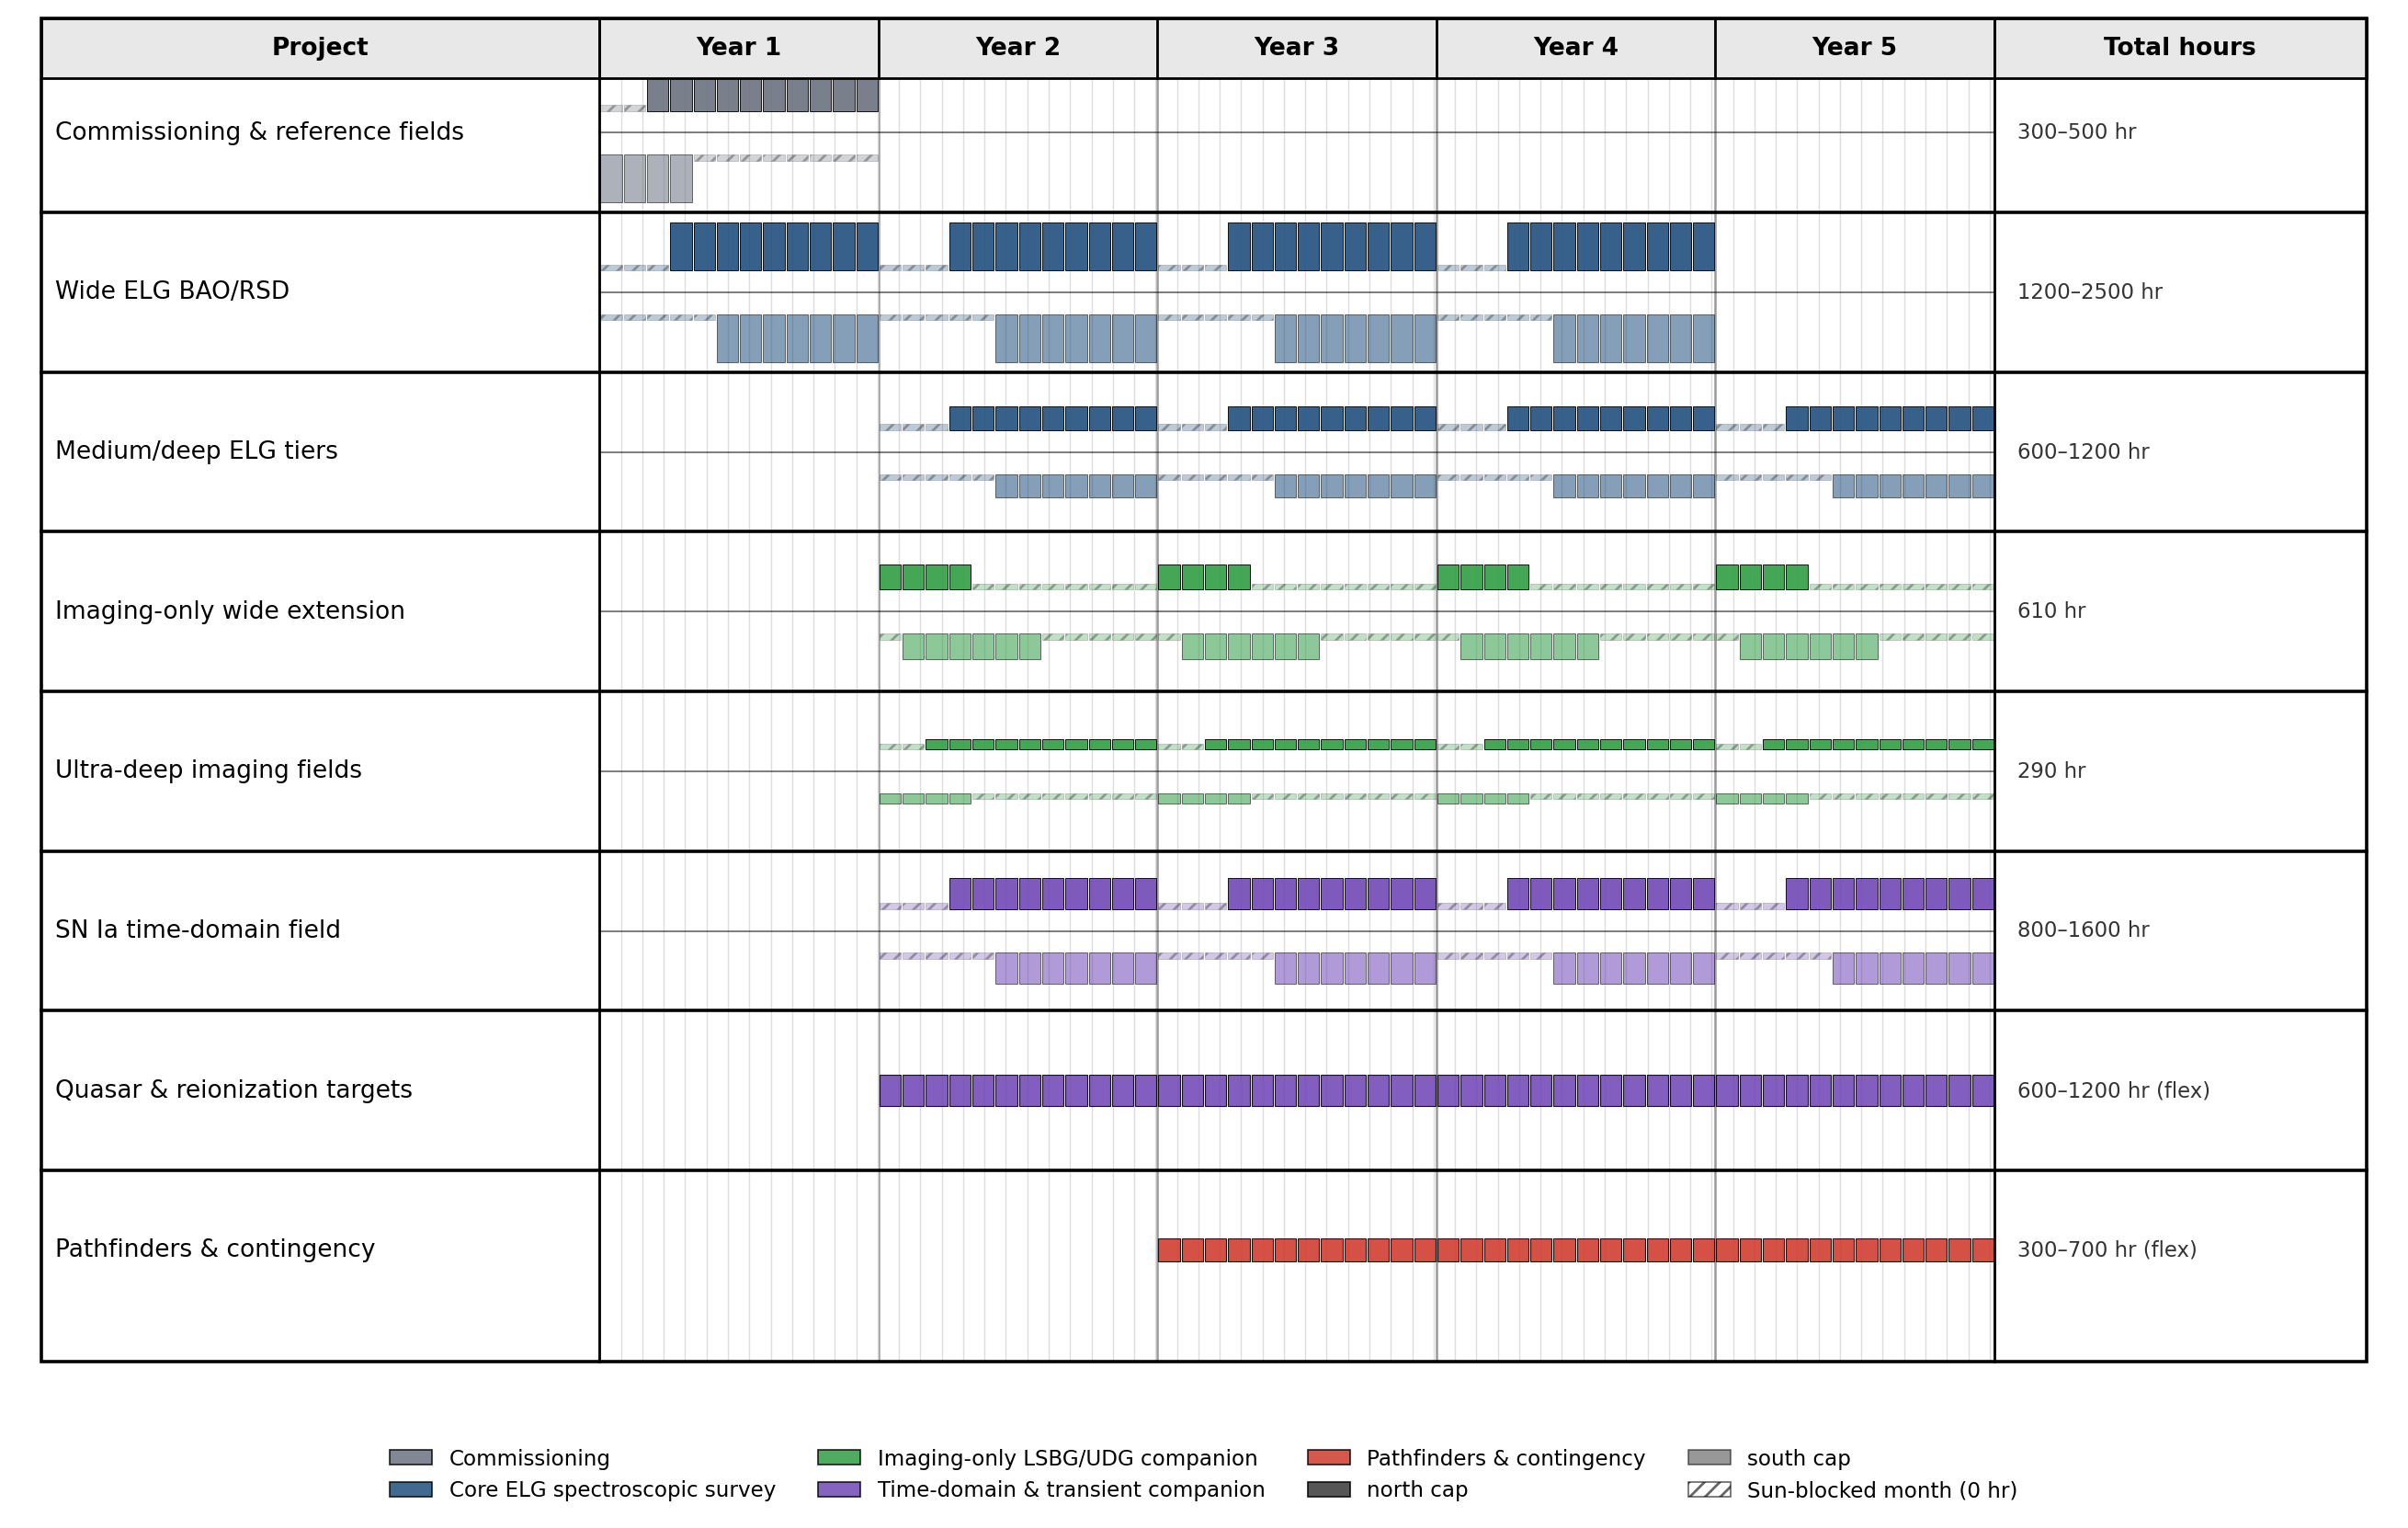
\includegraphics[width=\textwidth]{survey_timeline_gantt.png}
\caption{Table~\ref{tab:timeline}'s observing-program envelope, redrawn as a table (Project, Year~1--5, Total~hours columns, with a bold rule between programs) against a month-by-month field-of-regard model rather than as flat year-range bars. An L2 halo orbit is assumed, matching the JWST-heritage cosmic-ray-rate assumption already used in the ETC (Section~\ref{sec:etc}), together with a Euclid/Roman-style field of regard restricting pointing to a $64^\circ$--$116^\circ$ ($90^\circ\pm26^\circ$) solar-elongation band. Both are introduced here as an illustrative benchmark for this figure alone, not as an adopted mission parameter. Each row's real target field or field pair is tested against this band on the 15th of every month. These are the Bo\"otes and SXDS/UDS/XMM-LSS wide-tier anchors, the Lockman Hole and south Galactic pole imaging-only extensions, the two ultra-deep fields, and the paired SN~Ia cadence fields. A north and a south cap are drawn as separate sub-bars, north solid and south lighter and separated by a thin rule, because the two hemispheres of a given program become Sun-visible in different months. Bar thickness is each cap's share of the row's quoted science-time range (Table~\ref{tab:timeline} midpoint), divided evenly across the months where that cap is Sun-visible within its quoted Year span, on one linear hours-per-month scale shared by every bar in the figure, single or split. A hatched sliver marks a month inside that span where the cap is instead Sun-blocked, carrying zero hours. The quasar/reionization and pathfinder rows draw from flexible target lists without fixed coordinates. Therefore, no field-of-regard split applies to them, and they keep a single, evenly distributed bar on the same scale. Because every bar shares one scale, thickness can be compared and summed directly across rows. The combined hours of every row active in the same calendar month never exceed 177~hr, well inside the $\sim$672~hr of telescope time physically available in a 4-week block. Therefore, a thick bar always reads as more allocated hours within that fixed-width month, never as borrowed calendar time. As in Table~\ref{tab:timeline} itself, the year ranges remain an existence proof rather than a committed schedule, and each row's monthly allocation is computed independently of the others. Therefore, this figure does not yet resolve the rows into a single shared-telescope schedule.}
\label{fig:surveytimeline}
\end{figure}

\section*{Figures and Sources}
Most schematic figures in this document are generated directly in \LaTeX\ using TikZ. Figure~\ref{fig:crowded} is a slitless scene simulation generated locally at the baseline instrument parameters with the tracked script \texttt{make\_slitless\_scene\_sim.py}, using the repository's FSPS galaxy templates as source spectra. Figure~\ref{fig:slicer} is generated locally with the tracked script \texttt{make\_hsc\_slicer\_demo.py}, using the same instrument parameters and FSPS templates as Figure~\ref{fig:crowded}, but with source positions, brightnesses, sizes, ellipticities, and position angles measured from a real Subaru HSC-SSP deep image of the SXDS/UDS/XMM-LSS anchor \cite{aihara2018} instead of a synthetic population. Figure~\ref{fig:elgspectrum} uses an observed bright SDSS DR17 low-redshift emission-line galaxy spectrum converted to a local plotting table. Figure~\ref{fig:elgobswavez} stacks actual SDSS/BOSS and DESI DR1 spectra retrieved through SPARCL together with HST WFC3/G141 3D-HST COSMOS grism spectra (v4.1.5 1D extractions) and JWST/NIRSpec PRISM star-forming galaxy spectra (msaexp 1D extractions from the DAWN JWST Archive) on an approximately uniform display grid in redshift, spanning the full $0.36$--$3.0\,\mu$m proposed range. Figures~\ref{fig:elgmagdepth} and \ref{fig:desiMlf} use the DESI DR1 LSS ELG catalog with an observed-frame absolute magnitude computed locally from the downloaded FITS table. In Figure~\ref{fig:desiMlf} the binned observed-frame luminosity function is additionally fit with a Schechter function on the bright side of each redshift bin and shown as smooth curves. Figure~\ref{fig:phillips} plots the real Carnegie Supernova Project\,I sample of 139 SNe Ia (Burns et~al.\ \cite{burns2018csp}, VizieR catalog J/ApJ/869/56), computing the host-extinction-corrected peak absolute magnitude $M_V=V_{\max}-\mu_{\rm CV}-R_V\,E(B\!-\!V)$ from the tabulated distance modulus and reddening, plotting it against the tabulated $\Delta m_{15}(B)$, and overlaying a quadratic Phillips relation fitted locally to those points. The figure layout follows Figure 11 of Zeng et~al.\ \cite{zeng2025sn2023ehl}. Figure~\ref{fig:uvtwins} plots the observed flux-calibrated Swift/UVOT UV-grism spectra of SN\,2011fe and SN\,2011by near maximum, retrieved from the Open Supernova Catalog archive \cite{guillochon2017}, deredshifted and scaled over the optical. Figure~\ref{fig:sniacosmo} (the multi-cosmology SN Ia Hubble diagram with current and target Hubble-residual scatter) is generated locally with \texttt{astropy} distance moduli for the four cosmologies against the real Pantheon$+$SH0ES sample \cite{brout2022}, retaining the 1580 Hubble-flow SNe Ia ($z>0.01$, Cepheid calibrators removed). Figure~\ref{fig:nuvband} is generated in TikZ and shows the redshifting of fixed rest-frame wavelengths into the proposed observed band. Figure~\ref{fig:lyathreshold} is computed locally, integrating a Voigt profile to obtain the Ly$\alpha$ curve of growth and inverting it against the $R=1000$ detection limit of Eq.~\eqref{eq:wmin} to give the minimum detectable H\,\textsc{i} column density. Figure~\ref{fig:lya3dexternal} is an external CLAMATO 3D Ly$\alpha$ forest tomography rendering from the arXiv source package. Figure~\ref{fig:hr4xi} combines an observed BOSS CMASS-North pair-count measurement (obscorr pipeline, the same source data behind \texttt{plot\_bao\_jk.py}) with the author's Horizon Run 4 mock $\xi(\sigma,\pi)$ pair-count measurement in redshift space, rather than reproducing any published figure. Figures~\ref{fig:sidmsigmav} and \ref{fig:fdmslice} are the original figures from the arXiv source packages of Kaplinghat, Tulin \& Yu \cite{kaplinghat2016} and Schive et~al.\ \cite{schive2014}, reproduced as published and marked courtesy in their captions, because the underlying per-system cross-section fits and wave-simulation data are not public. Figure~\ref{fig:sparcdiv} is drawn locally from the public SPARC mass-model files \cite{lelli2016}. Figure~\ref{fig:fdmconstraints} is drawn locally from the published bounds quoted in its caption. Figures~\ref{fig:cirrusfil} and \ref{fig:cirruscolors} are the original figures from the arXiv source package of Rom\'an, Trujillo \& Montes \cite{roman2020}, reproduced as published and marked courtesy in their captions, because the processed deep mosaics and per-field cirrus colour measurements behind them are not public. Figure~\ref{fig:hr5gsmf} is the original figure from the arXiv source package of the team's own Horizon Run 5 stellar-mass-function study \cite{kim2023gsmf}, reproduced as published. Figure~\ref{fig:surveytimeline} is generated locally with the tracked script \texttt{make\_survey\_timeline.py}, combining Table~\ref{tab:timeline}'s quoted science-time ranges and real target-field coordinates with an \texttt{astropy} Sun-position calculation, under the illustrative L2/Euclid-Roman-style field-of-regard assumption stated in its caption. Literature and documentation sources are listed below.

\clearpage
\begin{thebibliography}{99}
\bibitem{cess2024}
X. Wang et al.,
``CSST Large-scale Structure Analysis Pipeline: II. the CSST Emulator for Slitless Spectroscopy,''
\emph{Monthly Notices of the Royal Astronomical Society}, 528, 2770, 2024.
\url{https://arxiv.org/html/2401.04171v2}
\doi{10.1093/mnras/stae157}

\bibitem{jwstdocs}
Space Telescope Science Institute,
``NIRCam Grisms -- JWST User Documentation.''
\url{https://jwst-docs.stsci.edu/jwst-near-infrared-camera/nircam-instrumentation/nircam-grisms}

\bibitem{jdoxnircamsens}
Space Telescope Science Institute,
``NIRCam Imaging Sensitivity -- JWST User Documentation.''
\url{https://jwst-docs.stsci.edu/jwst-near-infrared-camera/nircam-performance/nircam-sensitivity}

\bibitem{jdoxnirspecsens}
Space Telescope Science Institute,
``NIRSpec Sensitivity -- JWST User Documentation.''
\url{https://jwst-docs.stsci.edu/jwst-near-infrared-spectrograph/nirspec-performance/nirspec-sensitivity}

\bibitem{wang2021}
Y. Wang et al.,
``The High Latitude Spectroscopic Survey on the Nancy Grace Roman Space Telescope,''
\emph{The Astrophysical Journal}, 928, 1, 2022.
\url{https://arxiv.org/abs/2110.01829}
\doi{10.3847/1538-4357/ac4973}

\bibitem{euclid2011}
R. Laureijs et al.,
``Euclid Definition Study Report,'' (Euclid Red Book; NISP slitless-grism H$\alpha$ flux limit $\simeq3.5$--$4\times10^{-16}\,{\rm erg\,s^{-1}\,cm^{-2}}$ at $3.5\sigma$),
\emph{arXiv:1110.3193}, 2011.
\url{https://arxiv.org/abs/1110.3193}
\doi{10.48550/arXiv.1110.3193}

\bibitem{scaramella2022}
Euclid Collaboration: R. Scaramella et al.,
``Euclid preparation. I. The Euclid Wide Survey,''
\emph{Astronomy \& Astrophysics}, 662, A112, 2022.
\url{https://arxiv.org/abs/2108.01201}
\doi{10.1051/0004-6361/202141938}

\bibitem{romandocs}
Space Telescope Science Institute,
``High-Latitude Wide-Area Survey -- Roman User Documentation.''
\url{https://roman-docs.stsci.edu/roman-community-defined-surveys/high-latitude-wide-area-survey}

\bibitem{hr4}
J. Kim, C. Park, B. L'Huillier, and S. E. Hong,
``Horizon Run 4 Simulation: Coupled Evolution of Galaxies and Large-scale Structures of the Universe,''
\emph{Journal of Korean Astronomical Society}, 48, 213, 2015.
\url{https://arxiv.org/abs/1508.05107}
\doi{10.5303/JKAS.2015.48.4.213}

\bibitem{landyszalay1993}
S. D. Landy and A. S. Szalay,
``Bias and variance of angular correlation functions,''
\emph{The Astrophysical Journal}, 412, 64, 1993.
\doi{10.1086/172900}

\bibitem{fkp1994}
H. A. Feldman, N. Kaiser, and J. A. Peacock,
``Power-spectrum analysis of three-dimensional redshift surveys,''
\emph{The Astrophysical Journal}, 426, 23, 1994.
\url{https://arxiv.org/abs/astro-ph/9304022}
\doi{10.1086/174036}

\bibitem{yamamoto2006}
K. Yamamoto, M. Nakamichi, A. Kamino, B. A. Bassett, and H. Nishioka,
``A Measurement of the Quadrupole Power Spectrum in the Clustering of the 2dF QSO Survey,''
\emph{Publications of the Astronomical Society of Japan}, 58, 93, 2006.
\url{https://arxiv.org/abs/astro-ph/0505115}
\doi{10.1093/pasj/58.1.93}

\bibitem{hand2017nbodykit}
N. Hand, Y. Feng, Y. Li, U. Seljak, Z. Slepian, and F. Beutler,
``nbodykit: an open-source, massively parallel toolkit for large-scale structure,''
\emph{The Astronomical Journal}, 156, 160, 2018.
\url{https://arxiv.org/abs/1712.05834}
\doi{10.3847/1538-3881/aadae0}

\bibitem{bolton2012}
A. S. Bolton et al.,
``Spectral Classification and Redshift Measurement for the SDSS-III Baryon Oscillation Spectroscopic Survey,''
\emph{The Astronomical Journal}, 144, 144, 2012.
\url{https://arxiv.org/abs/1207.7326}
\doi{10.1088/0004-6256/144/5/144}

\bibitem{quasarnet2018}
N. Busca and C. Balland,
``QuasarNET: Human-level spectral classification and redshifting with Deep Neural Networks,''
\emph{arXiv:1808.09955}, 2018.
\url{https://arxiv.org/abs/1808.09955}
\doi{10.48550/arXiv.1808.09955}

\bibitem{emcee2013}
D. Foreman-Mackey, D. W. Hogg, D. Lang, and J. Goodman,
``emcee: The MCMC Hammer,''
\emph{Publications of the Astronomical Society of the Pacific}, 125, 306, 2013.
\url{https://arxiv.org/abs/1202.3665}
\doi{10.1086/670067}

\bibitem{lewisbridle2002}
A. Lewis and S. Bridle,
``Cosmological parameters from CMB and other data: A Monte Carlo approach,''
\emph{Physical Review D}, 66, 103511, 2002.
\url{https://arxiv.org/abs/astro-ph/0205436}
\doi{10.1103/PhysRevD.66.103511}

\bibitem{torradolewis2021}
J. Torrado and A. Lewis,
``Cobaya: Code for Bayesian Analysis of hierarchical physical models,''
\emph{Journal of Cosmology and Astroparticle Physics}, 2021, 057, 2021.
\url{https://arxiv.org/abs/2005.05290}
\doi{10.1088/1475-7516/2021/05/057}

\bibitem{polychord2015}
W. J. Handley, M. P. Hobson, and A. N. Lasenby,
``POLYCHORD: next-generation nested sampling,''
\emph{Monthly Notices of the Royal Astronomical Society}, 453, 4384, 2015.
\url{https://arxiv.org/abs/1506.00171}
\doi{10.1093/mnras/stv1911}

\bibitem{cosmopower2022}
A. Spurio Mancini, D. Piras, J. Alsing, B. Joachimi, and M. P. Hobson,
``CosmoPower: emulating cosmological power spectra for accelerated Bayesian inference from next-generation surveys,''
\emph{Monthly Notices of the Royal Astronomical Society}, 511, 1771, 2022.
\url{https://arxiv.org/abs/2106.03846}
\doi{10.1093/mnras/stac064}

\bibitem{euclidemulator2021}
M. Knabenhans et al.,
``Euclid preparation: IX. EuclidEmulator2 -- power spectrum emulation with massive neutrinos and self-consistent dark energy perturbations,''
\emph{Monthly Notices of the Royal Astronomical Society}, 505, 2840, 2021.
\url{https://arxiv.org/abs/2010.11288}
\doi{10.1093/mnras/stab1366}

\bibitem{cranmer2020}
K. Cranmer, J. Brehmer, and G. Louppe,
``The frontier of simulation-based inference,''
\emph{Proceedings of the National Academy of Sciences}, 117, 30055, 2020.
\url{https://arxiv.org/abs/1911.01429}
\doi{10.1073/pnas.1912789117}

\bibitem{raichoor2022}
A. Raichoor et al.,
``Target Selection and Validation of DESI Emission Line Galaxies,''
\emph{The Astronomical Journal}, 165, 126, 2023.
\url{https://arxiv.org/abs/2208.08513}
\doi{10.3847/1538-3881/acb213}

\bibitem{desidr1}
DESI Collaboration: M. Abdul Karim et al.,
``Data Release 1 of the Dark Energy Spectroscopic Instrument,''
\emph{The Astronomical Journal}, 171, 285, 2026.
\url{https://arxiv.org/abs/2503.14745}
\doi{10.3847/1538-3881/ae4c43}

\bibitem{sparcl2024}
S. Juneau et al.,
``SPARCL: SPectra Analysis and Retrievable Catalog Lab,''
\emph{arXiv:2401.05576}, 2024.
\url{https://arxiv.org/abs/2401.05576}
\doi{10.48550/arXiv.2401.05576}

\bibitem{brammer2012}
G. B. Brammer et al.,
``3D-HST: A Wide-Field Grism Spectroscopic Survey with the Hubble Space Telescope,''
\emph{The Astrophysical Journal Supplement Series}, 200, 13, 2012.
\url{https://arxiv.org/abs/1204.2829}
\doi{10.1088/0067-0049/200/2/13}

\bibitem{momcheva2016}
I. G. Momcheva et al.,
``The 3D-HST Survey: Hubble Space Telescope WFC3/G141 Grism Spectra, Redshifts, and Emission Line Measurements for $\sim$100,000 Galaxies,''
\emph{The Astrophysical Journal Supplement Series}, 225, 27, 2016.
\url{https://arxiv.org/abs/1510.02106}
\doi{10.3847/0067-0049/225/2/27}

\bibitem{degraaff2024}
A. de Graaff et al.,
``RUBIES: a complete census of the bright and red distant Universe with JWST/NIRSpec'' and the associated \texttt{msaexp} NIRSpec reductions distributed through the DAWN JWST Archive (DJA),
\emph{Astronomy \& Astrophysics}, 697, A189, 2025.
\url{https://arxiv.org/abs/2409.05948}
\doi{10.1051/0004-6361/202452186}

\bibitem{heintz2023}
K. E. Heintz et al.,
``Dilution of chemical enrichment in galaxies 600 Myr after the Big Bang'' (DAWN JWST Archive NIRSpec data products),
\emph{Nature Astronomy}, 2023.
\url{https://arxiv.org/abs/2212.02890}
\doi{10.1038/s41550-023-02078-7}

\bibitem{comparat2015}
J. Comparat et al.,
``The 0.1$<z<$1.65 evolution of the bright end of the [OII] luminosity function,''
\emph{Astronomy \& Astrophysics}, 575, A40, 2015.
\url{https://arxiv.org/abs/1408.1523}
\doi{10.1051/0004-6361/201424767}

\bibitem{comparat2016}
J. Comparat et al.,
``The evolution of the [OII], H$\beta$ and [OIII] emission-line luminosity functions over the last nine billions years,''
\emph{Monthly Notices of the Royal Astronomical Society}, 461, 1076, 2016.
\url{https://arxiv.org/abs/1605.02875}
\doi{10.1093/mnras/stw1393}

\bibitem{schechter1976}
P. Schechter,
``An analytic expression for the luminosity function for galaxies,''
\emph{The Astrophysical Journal}, 203, 297, 1976.
\url{https://ui.adsabs.harvard.edu/abs/1976ApJ...203..297S/abstract}
\doi{10.1086/154079}

\bibitem{saito2020}
S. Saito et al.,
``The Synthetic Emission Line COSMOS catalog: H$\alpha$ and [OII] galaxy luminosity functions and counts at $0.3<z<2.5$,''
\emph{Monthly Notices of the Royal Astronomical Society}, 494, 199, 2020.
\url{https://arxiv.org/abs/2003.06394}
\doi{10.1093/mnras/staa727}

\bibitem{mehta2015}
V. Mehta et al.,
``Predicting the redshift 2 H$\alpha$ luminosity function using [OIII] emission line galaxies,''
\emph{The Astrophysical Journal}, 811, 141, 2015.
\url{https://arxiv.org/abs/1505.07843}
\doi{10.1088/0004-637X/811/2/141}

\bibitem{khostovan2015}
A. A. Khostovan et al.,
``The Evolution of the H$\beta$+[OIII] and [OII] Luminosity Functions and Star Formation History of the Universe up to $z\sim5$ from HiZELS,''
\emph{Monthly Notices of the Royal Astronomical Society}, 452, 3948, 2015.
\url{https://arxiv.org/abs/1503.00004}
\doi{10.1093/mnras/stv1474}

\bibitem{newman2013deep2}
J. A. Newman et al.,
``The DEEP2 Galaxy Redshift Survey: Design, Observations, Data Reduction, and Redshifts,''
\emph{The Astrophysical Journal Supplement Series}, 208, 5, 2013.
\url{https://arxiv.org/abs/1203.3192}
\doi{10.1088/0067-0049/208/1/5}

\bibitem{lefevre2013vvds}
O. Le F\`evre et al.,
``The VIMOS VLT Deep Survey final data release: a spectroscopic sample of 35016 galaxies and AGN out to $z\sim6.7$ selected with $17.5\le i_{\rm AB}\le24.7$,''
\emph{Astronomy \& Astrophysics}, 559, A14, 2013.
\url{https://arxiv.org/abs/1307.0545}
\doi{10.1051/0004-6361/201322179}

\bibitem{knobel2012zcosmos}
C. Knobel et al.,
``The zCOSMOS 20k Group Catalog,''
\emph{The Astrophysical Journal}, 753, 121, 2012.
\url{https://arxiv.org/abs/1207.0002}
\doi{10.1088/0004-637X/753/2/121}

\bibitem{astraatmadja2026}
T. L. Astraatmadja et al.,
``Three-dimensional scene reconstruction using Roman slitless spectra,''
\emph{arXiv:2601.05233}, 2026.
\url{https://arxiv.org/abs/2601.05233}
\doi{10.3847/1538-4357/ae355e}

\bibitem{tdcosmo2025}
A. J. Shajib et al.,
``TDCOSMO XXIV. First spatially resolved kinematics of the lens galaxy obtained using JWST-NIRSpec to improve time-delay cosmography,''
\emph{arXiv:2506.21665}, 2025.
\url{https://arxiv.org/html/2506.21665v1}
\doi{10.48550/arXiv.2506.21665}

\bibitem{chaves2026}
J. Chaves-Montero et al.,
``Cosmological analysis of the DESI DR1 Lyman alpha 1D power spectrum,''
\emph{arXiv:2601.21432}, 2026.
\url{https://arxiv.org/abs/2601.21432}
\doi{10.48550/arXiv.2601.21432}

\bibitem{lee2018clamato}
K.-G. Lee et al.,
``First Data Release of the COSMOS Lyman-Alpha Mapping And Tomography Observations: 3D Lyman-$\alpha$ Forest Tomography at $2.05<z<2.55$,''
\emph{The Astrophysical Journal Supplement Series}, 237, 31, 2018.
\url{https://arxiv.org/abs/1710.02894}
\doi{10.3847/1538-4365/aace58}

\bibitem{mortlock2024}
L. Lenz, D. J. Mortlock, B. Leistedt, R. Barnett, and P. C. Hewett,
``An automated method for finding the most distant quasars,''
\emph{arXiv:2408.12770}, 2024.
\url{https://arxiv.org/html/2408.12770v2}
\doi{10.33232/001c.142765}

\bibitem{sdssdr17}
Abdurro'uf et al.,
``The Seventeenth Data Release of the Sloan Digital Sky Surveys: Complete Release of MaNGA, MaStar and APOGEE-2 Data,''
\emph{The Astrophysical Journal Supplement Series}, 259, 35, 2022.
\url{https://www.sdss4.org/dr17/}
\doi{10.3847/1538-4365/ac4414}

\bibitem{kamann2013}
S. Kamann, L. Wisotzki, and M. M. Roth,
``Resolving stellar populations with crowded field 3D spectroscopy,''
\emph{Astronomy \& Astrophysics}, 549, A71, 2013.
\url{https://arxiv.org/abs/1211.0445}
\doi{10.1051/0004-6361/201220476}

\bibitem{husser2016}
T.-O. Husser et al.,
``MUSE crowded field 3D spectroscopy of over 12,000 stars in the globular cluster NGC 6397,''
\emph{Astronomy \& Astrophysics}, 588, A148, 2016.
\url{https://arxiv.org/abs/1602.01649}
\doi{10.1051/0004-6361/201526949}

\bibitem{axe2009}
M. K{\"u}mmel, J. R. Walsh, N. Pirzkal, H. Kuntschner, and A. Pasquali,
``The Slitless Spectroscopy Data Extraction Software aXe,''
\emph{Publications of the Astronomical Society of the Pacific}, 121, 59, 2009.
\url{https://arxiv.org/abs/0812.1434}
\doi{10.1086/596715}

\bibitem{linear2018}
R. E. Ryan Jr., S. Casertano, and N. Pirzkal,
``LINEAR: A Novel Algorithm for Reconstructing Slitless Spectroscopy from HST/WFC3,''
\emph{Publications of the Astronomical Society of the Pacific}, 130, 034501, 2018.
\url{https://arxiv.org/abs/1801.03936}
\doi{10.1088/1538-3873/aaa53e}

\bibitem{boker2022}
T. B\"oker, P. Ferruit, S. Birkmann, et al.,
``The Near-Infrared Spectrograph (NIRSpec) on the James Webb Space Telescope. IV. Capabilities and predicted performance for the NIRSpec IFU mode,''
\emph{Astronomy \& Astrophysics}, 661, A82, 2022.
\url{https://arxiv.org/abs/2202.03434}

\bibitem{burke2019}
C. J. Burke et al.,
``Deblending and Classifying Astronomical Sources with Mask R-CNN Deep Learning,''
\emph{Monthly Notices of the Royal Astronomical Society}, 490, 3952, 2019.
\url{https://arxiv.org/abs/1908.02748}
\doi{10.1093/mnras/stz2845}

\bibitem{liu2021}
R. Liu, J. D. McAuliffe, and J. Regier,
``Variational Inference for Deblending Crowded Starfields,''
\emph{arXiv:2102.02409}, 2021.
\url{https://arxiv.org/abs/2102.02409}
\doi{10.48550/arXiv.2102.02409}

\bibitem{horstman2022}
K. Horstman et al.,
``Using Non-Negative Matrix Factorization to Improve Calibration of the Keck OSIRIS Integral Field Spectrograph,''
\emph{Publications of the Astronomical Society of the Pacific}, 134, 064504, 2022.
\url{https://arxiv.org/abs/2206.04070}
\doi{10.1088/1538-3873/ac7905}

\bibitem{phillips1993}
M. M. Phillips,
``The Absolute Magnitudes of Type IA Supernovae,''
\emph{The Astrophysical Journal Letters}, 413, L105, 1993.
\url{https://ui.adsabs.harvard.edu/abs/1993ApJ...413L.105P}
\doi{10.1086/186970}

\bibitem{zeng2025sn2023ehl}
X. Zeng et al.,
``SN 2023ehl: A Normal Type Ia Supernova with High-velocity Features,''
\emph{The Astrophysical Journal}, 986, 68, 2025.
\url{https://doi.org/10.3847/1538-4357/adcf1b}
\doi{10.3847/1538-4357/adcf1b}

\bibitem{burns2018csp}
C. R. Burns et al.,
``The Carnegie Supernova Project: Absolute Calibration and the Hubble Constant,''
\emph{The Astrophysical Journal}, 869, 56, 2018.
\url{https://doi.org/10.3847/1538-4357/aae51c}
\doi{10.3847/1538-4357/aae51c}

\bibitem{foleykirshner2013}
R. J. Foley and R. P. Kirshner,
``Metallicity Differences in Type Ia Supernova Progenitors Inferred from Ultraviolet Spectra,''
\emph{The Astrophysical Journal Letters}, 769, L1, 2013.
\url{https://arxiv.org/abs/1304.0780}
\doi{10.1088/2041-8205/769/1/L1}

\bibitem{graham2015}
M. L. Graham et al.,
``Twins for life: a comparative analysis of the Type Ia supernovae 2011fe and 2011by,''
\emph{Monthly Notices of the Royal Astronomical Society}, 446, 2073, 2015.
\url{https://arxiv.org/abs/1408.2651}
\doi{10.1093/mnras/stu2221}

\bibitem{lentz2000}
E. J. Lentz, E. Baron, D. Branch, P. H. Hauschildt, and P. E. Nugent,
``Metallicity Effects in Non-LTE Model Atmospheres of Type Ia Supernovae,''
\emph{The Astrophysical Journal}, 530, 966, 2000.
\url{https://arxiv.org/abs/astro-ph/9906016}
\doi{10.1086/308400}

\bibitem{milne2015}
P. A. Milne et al.,
``The Changing Fractions of Type Ia Supernova NUV-Optical Subclasses with Redshift,''
\emph{The Astrophysical Journal}, 803, 20, 2015.
\url{https://arxiv.org/abs/1408.1706}
\doi{10.1088/0004-637X/803/1/20}

\bibitem{riess1998}
A. G. Riess et al.,
``Observational Evidence from Supernovae for an Accelerating Universe and a Cosmological Constant,''
\emph{The Astronomical Journal}, 116, 1009, 1998.
\url{https://arxiv.org/abs/astro-ph/9805201}
\doi{10.1086/300499}

\bibitem{perlmutter1999}
S. Perlmutter et al.,
``Measurements of $\Omega$ and $\Lambda$ from 42 High-Redshift Supernovae,''
\emph{The Astrophysical Journal}, 517, 565, 1999.
\url{https://arxiv.org/abs/astro-ph/9812133}
\doi{10.1086/307221}

\bibitem{wang2009}
X. Wang et al.,
``Improved Distances to Type Ia Supernovae with Two Spectroscopic Subclasses,''
\emph{The Astrophysical Journal Letters}, 699, L139, 2009.
\url{https://arxiv.org/abs/0906.1616}
\doi{10.1088/0004-637X/699/2/L139}

\bibitem{riess2004}
A. G. Riess et al.,
``Type Ia Supernova Discoveries at $z>1$ from the Hubble Space Telescope: Evidence for Past Deceleration and Constraints on Dark Energy Evolution,''
\emph{The Astrophysical Journal}, 607, 665, 2004.
\url{https://arxiv.org/abs/astro-ph/0402512}
\doi{10.1086/383612}

\bibitem{rose2021roman}
B. M. Rose et al.,
``A Reference Survey for Supernova Cosmology with the Nancy Grace Roman Space Telescope,''
\emph{arXiv:2111.03081}, 2021.
\url{https://arxiv.org/abs/2111.03081}

\bibitem{ivezic2019lsst}
{\v Z}. Ivezi{\'c} et al.,
``LSST: From Science Drivers to Reference Design and Anticipated Data Products,''
\emph{The Astrophysical Journal}, 873, 111, 2019.
\url{https://arxiv.org/abs/0805.2366}
\doi{10.3847/1538-4357/ab042c}

\bibitem{riess2022}
A. G. Riess et al.,
``A Comprehensive Measurement of the Local Value of the Hubble Constant with 1\,km\,s$^{-1}$\,Mpc$^{-1}$ Uncertainty from the Hubble Space Telescope and the SH0ES Team,''
\emph{The Astrophysical Journal Letters}, 934, L7, 2022.
\url{https://arxiv.org/abs/2112.04510}
\doi{10.3847/2041-8213/ac5c5b}

\bibitem{brout2022}
D. Brout et al.,
``The Pantheon+ Analysis: Cosmological Constraints,''
\emph{The Astrophysical Journal}, 938, 110, 2022.
\url{https://arxiv.org/abs/2202.04077}
\doi{10.3847/1538-4357/ac8e04}

\bibitem{planck2018}
Planck Collaboration (N. Aghanim et al.),
``Planck 2018 results. VI. Cosmological parameters,''
\emph{Astronomy \& Astrophysics}, 641, A6, 2020.
\url{https://arxiv.org/abs/1807.06209}
\doi{10.1051/0004-6361/201833910}

\bibitem{collett2015}
T. E. Collett,
``The Population of Galaxy-Galaxy Strong Lenses in Forthcoming Optical Imaging Surveys,''
\emph{The Astrophysical Journal}, 811, 20, 2015.
\url{https://arxiv.org/abs/1507.02657}
\doi{10.1088/0004-637X/811/1/20}

\bibitem{weiner2020}
C. Weiner, S. Serjeant, and C. Sedgwick,
``Predictions for Strong-lens Detections with the Nancy Grace Roman Space Telescope,''
\emph{Research Notes of the AAS}, 4, 190, 2020.
\url{https://arxiv.org/abs/2010.15173}
\doi{10.3847/2515-5172/abc4ea}

\bibitem{walmsley2025}
Euclid Collaboration (M. Walmsley et al.),
``Euclid Quick Data Release (Q1): The Strong Lensing Discovery Engine A -- System overview and first lens sample,''
\emph{Astronomy \& Astrophysics}, 711, A26, 2026.
\url{https://arxiv.org/abs/2503.15324}
\doi{10.1051/0004-6361/202555141}

\bibitem{shu2025}
Y. Shu et al.,
``Confirming HSC Strong Lens Candidates with DESI Spectroscopy. I. Project Overview and First Results,''
\emph{Science China Physics, Mechanics \& Astronomy}, 68, 129511, 2025.
\url{https://arxiv.org/abs/2505.16158}
\doi{10.1007/s11433-025-2747-4}

\bibitem{collettauger2014}
T. E. Collett and M. W. Auger,
``Cosmological constraints from the double source plane lens SDSSJ0946$+$1006,''
\emph{Monthly Notices of the Royal Astronomical Society}, 443, 969, 2014.
\url{https://arxiv.org/abs/1403.5278}
\doi{10.1093/mnras/stu1190}

\bibitem{collett2012}
T. E. Collett, M. W. Auger, V. Belokurov, P. J. Marshall, and A. C. Hall,
``Constraining the dark energy equation of state with double-source-plane strong lenses,''
\emph{Monthly Notices of the Royal Astronomical Society}, 424, 2864, 2012.
\url{https://arxiv.org/abs/1203.2758}
\doi{10.1111/j.1365-2966.2012.21424.x}

\bibitem{sahu2025}
N. Sahu et al.,
``Cosmography with the Double-source-plane Strong Gravitational Lens AGEL150745$+$052256,''
\emph{The Astrophysical Journal}, 991, 72, 2025.
\url{https://arxiv.org/abs/2504.00656}
\doi{10.3847/1538-4357/adf442}

\bibitem{bowden2025}
D. J. Bowden et al.,
``Constraining Cosmology with Double-source-plane Strong Gravitational Lenses from the AGEL Survey,''
\emph{The Astrophysical Journal}, 993, 124, 2025.
\url{https://arxiv.org/abs/2509.15012}
\doi{10.3847/1538-4357/ae092e}

\bibitem{koopmans2009}
L. V. E. Koopmans et al.,
``The Structure and Dynamics of Massive Early-type Galaxies: On Homology, Isothermality, and Isotropy Inside One Effective Radius,''
\emph{The Astrophysical Journal Letters}, 703, L51, 2009.
\url{https://arxiv.org/abs/0906.1349}
\doi{10.1088/0004-637X/703/1/L51}

\bibitem{auger2010}
M. W. Auger et al.,
``The Sloan Lens ACS Survey. X. Stellar, Dynamical, and Total Mass Correlations of Massive Early-type Galaxies,''
\emph{The Astrophysical Journal}, 724, 511, 2010.
\url{https://arxiv.org/abs/1007.2880}
\doi{10.1088/0004-637X/724/1/511}

\bibitem{sonnenfeld2013}
A. Sonnenfeld et al.,
``The SL2S Galaxy-scale Lens Sample. IV. The Dependence of the Total Mass Density Profile of Early-type Galaxies on Redshift, Stellar Mass, and Size,''
\emph{The Astrophysical Journal}, 777, 98, 2013.
\url{https://arxiv.org/abs/1307.4759}
\doi{10.1088/0004-637X/777/2/98}

\bibitem{etherington2023}
A. Etherington et al.,
``Beyond the bulge--halo conspiracy? Density profiles of early-type galaxies from extended-source strong lensing,''
\emph{Monthly Notices of the Royal Astronomical Society}, 521, 6005, 2023.
\url{https://arxiv.org/abs/2207.04070}
\doi{10.1093/mnras/stad582}

\bibitem{wong2020}
K. C. Wong et al.,
``H0LiCOW XIII. A 2.4 per cent measurement of $H_0$ from lensed quasars: 5.3$\sigma$ tension between early- and late-Universe probes,''
\emph{Monthly Notices of the Royal Astronomical Society}, 498, 1420, 2020.
\url{https://arxiv.org/abs/1907.04869}
\doi{10.1093/mnras/stz3094}

\bibitem{birrer2020}
S. Birrer et al.,
``TDCOSMO IV. Hierarchical time-delay cosmography -- joint inference of the Hubble constant and galaxy density profiles,''
\emph{Astronomy \& Astrophysics}, 643, A165, 2020.
\url{https://arxiv.org/abs/2007.02941}
\doi{10.1051/0004-6361/202038861}

\bibitem{birrer2025}
S. Birrer et al.,
``TDCOSMO 2025: Cosmological constraints from strong lensing time delays,''
\emph{Astronomy \& Astrophysics}, 704, A63, 2025.
\url{https://arxiv.org/abs/2506.03023}
\doi{10.1051/0004-6361/202555801}

\bibitem{suyu2010}
S. H. Suyu et al.,
``Dissecting the Gravitational Lens B1608$+$656. II. Precision Measurements of the Hubble Constant, Spatial Curvature, and the Dark Energy Equation of State,''
\emph{The Astrophysical Journal}, 711, 201, 2010.
\url{https://arxiv.org/abs/0910.2773}
\doi{10.1088/0004-637X/711/1/201}

\bibitem{rusu2017}
C. E. Rusu et al.,
``H0LiCOW III. Quantifying the effect of mass along the line of sight to the gravitational lens HE\,0435$-$1223 through weighted galaxy counts,''
\emph{Monthly Notices of the Royal Astronomical Society}, 467, 4220, 2017.
\url{https://arxiv.org/abs/1607.01047}
\doi{10.1093/mnras/stx285}

\bibitem{wells2023}
P. Wells, C. D. Fassnacht, and C. E. Rusu,
``TDCOSMO XIV: Practical techniques for estimating external convergence of strong gravitational lens systems and applications to the SDSS\,J0924$+$0219 system,''
\emph{Astronomy \& Astrophysics}, 676, A95, 2023.
\url{https://arxiv.org/abs/2302.03176}
\doi{10.1051/0004-6361/202346093}

\bibitem{greene2013}
Z. S. Greene et al.,
``Improving the Precision of Time-delay Cosmography with Observations of Galaxies along the Line of Sight,''
\emph{The Astrophysical Journal}, 768, 39, 2013.
\url{https://arxiv.org/abs/1303.3588}
\doi{10.1088/0004-637X/768/1/39}

\bibitem{metcalf2019}
R. B. Metcalf et al.,
``The Strong Gravitational Lens Finding Challenge,''
\emph{Astronomy \& Astrophysics}, 625, A119, 2019.
\url{https://arxiv.org/abs/1802.03609}
\doi{10.1051/0004-6361/201832797}

\bibitem{jacobs2019}
C. Jacobs et al.,
``An Extended Catalog of Galaxy-Galaxy Strong Gravitational Lenses Discovered in DES Using Convolutional Neural Networks,''
\emph{The Astrophysical Journal Supplement Series}, 243, 17, 2019.
\url{https://arxiv.org/abs/1905.10522}
\doi{10.3847/1538-4365/ab26b6}

\bibitem{hezaveh2017}
Y. D. Hezaveh, L. Perreault Levasseur, and P. J. Marshall,
``Fast automated analysis of strong gravitational lenses with convolutional neural networks,''
\emph{Nature}, 548, 555, 2017.
\url{https://arxiv.org/abs/1708.08842}
\doi{10.1038/nature23463}

\bibitem{perreaultlevasseur2017}
L. Perreault Levasseur, Y. D. Hezaveh, and R. H. Wechsler,
``Uncertainties in Parameters Estimated with Neural Networks: Application to Strong Gravitational Lensing,''
\emph{The Astrophysical Journal Letters}, 850, L7, 2017.
\url{https://arxiv.org/abs/1708.08843}
\doi{10.3847/2041-8213/aa9704}

\bibitem{park2021}
J. W. Park et al.,
``Large-scale Gravitational Lens Modeling with Bayesian Neural Networks for Accurate and Precise Inference of the Hubble Constant,''
\emph{The Astrophysical Journal}, 910, 39, 2021.
\url{https://arxiv.org/abs/2012.00042}
\doi{10.3847/1538-4357/abdfc4}

\bibitem{wagnercarena2021}
S. Wagner-Carena et al.,
``Hierarchical Inference with Bayesian Neural Networks: An Application to Strong Gravitational Lensing,''
\emph{The Astrophysical Journal}, 909, 187, 2021.
\url{https://arxiv.org/abs/2010.13787}
\doi{10.3847/1538-4357/abdf59}

\bibitem{legin2023}
R. Legin, Y. Hezaveh, L. Perreault-Levasseur, and B. Wandelt,
``A Framework for Obtaining Accurate Posteriors of Strong Gravitational Lensing Parameters with Flexible Priors and Implicit Likelihoods Using Density Estimation,''
\emph{The Astrophysical Journal}, 943, 4, 2023.
\url{https://arxiv.org/abs/2212.00044}
\doi{10.3847/1538-4357/aca7c2}

\bibitem{chabanier2019}
S. Chabanier et al.,
``The one-dimensional power spectrum from the SDSS DR14 Ly$\alpha$ forests,''
\emph{Journal of Cosmology and Astroparticle Physics}, 07, 017, 2019.
\url{https://arxiv.org/abs/1812.03554}
\doi{10.1088/1475-7516/2019/07/017}

\bibitem{karacayli2025}
N. G. Kar\'a\c{c}ayl{\i} et al.,
``The DESI DR1 Lyman-$\alpha$ forest 1D power spectrum: the optimal estimator measurement,''
\emph{Journal of Cosmology and Astroparticle Physics}, 10, 004, 2025.
\url{https://arxiv.org/abs/2505.07974}
\doi{10.1088/1475-7516/2025/10/004}

\bibitem{ravoux2025}
C. Ravoux et al.,
``The DESI DR1 Lyman-$\alpha$ forest 1D power spectrum: the FFT estimator measurement,''
\emph{Journal of Cosmology and Astroparticle Physics}, 11, 079, 2025.
\url{https://arxiv.org/abs/2505.09493}
\doi{10.1088/1475-7516/2025/11/079}

\bibitem{viel2013}
M. Viel, G. D. Becker, J. S. Bolton, and M. G. Haehnelt,
``Warm dark matter as a solution to the small scale crisis: New constraints from high redshift Lyman-$\alpha$ forest data,''
\emph{Physical Review D}, 88, 043502, 2013.
\url{https://arxiv.org/abs/1306.2314}
\doi{10.1103/PhysRevD.88.043502}

\bibitem{irsic2017}
V. Ir\v{s}i\v{c} et al.,
``New constraints on the free-streaming of warm dark matter from intermediate and small scale Lyman-$\alpha$ forest data,''
\emph{Physical Review D}, 96, 023522, 2017.
\url{https://arxiv.org/abs/1702.01764}
\doi{10.1103/PhysRevD.96.023522}

\bibitem{walther2019}
M. Walther et al.,
``New constraints on IGM thermal evolution from the Ly$\alpha$ forest power spectrum,''
\emph{The Astrophysical Journal}, 872, 13, 2019.
\url{https://arxiv.org/abs/1808.04367}
\doi{10.3847/1538-4357/aafad1}

\bibitem{gaikwad2021}
P. Gaikwad et al.,
``Consistent and robust measurement of the thermal state of the IGM at $2\le z\le4$ from a large sample of Ly$\alpha$ forest spectra,''
\emph{Monthly Notices of the Royal Astronomical Society}, 506, 4389, 2021.
\url{https://arxiv.org/abs/2009.00016}
\doi{10.1093/mnras/stab2017}

\bibitem{newman2020latis}
A. B. Newman et al.,
``LATIS: The Ly$\alpha$ Tomography IMACS Survey,''
\emph{The Astrophysical Journal}, 891, 147, 2020.
\url{https://arxiv.org/abs/2002.10676}
\doi{10.3847/1538-4357/ab75ee}

\bibitem{lee2014tomo}
K.-G. Lee et al.,
``Ly$\alpha$ Forest Tomography from Background Galaxies: The First Megaparsec-Resolution Large-Scale Structure Map at $z>2$,''
\emph{The Astrophysical Journal Letters}, 795, L12, 2014.
\url{https://arxiv.org/abs/1409.5632}
\doi{10.1088/2041-8205/795/1/L12}

\bibitem{dumasdesbourboux2020}
H. du Mas des Bourboux et al.,
``The Completed SDSS-IV Extended Baryon Oscillation Spectroscopic Survey: Baryon Acoustic Oscillations with Ly$\alpha$ Forests,''
\emph{The Astrophysical Journal}, 901, 153, 2020.
\url{https://arxiv.org/abs/2007.08995}
\doi{10.3847/1538-4357/abb085}

\bibitem{desi2024lya}
DESI Collaboration (A. G. Adame et al.),
``DESI 2024 IV: Baryon Acoustic Oscillations from the Lyman Alpha Forest,''
\emph{Journal of Cosmology and Astroparticle Physics}, 01, 124, 2025.
\url{https://arxiv.org/abs/2404.03001}
\doi{10.1088/1475-7516/2025/01/124}

\bibitem{noterdaeme2012}
P. Noterdaeme et al.,
``Column density distribution and cosmological mass density of neutral gas: Sloan Digital Sky Survey-III Data Release 9,''
\emph{Astronomy \& Astrophysics}, 547, L1, 2012.
\url{https://arxiv.org/abs/1210.1213}
\doi{10.1051/0004-6361/201220259}

\bibitem{parks2018}
D. Parks et al.,
``Deep learning of quasar spectra to discover and characterize damped Ly$\alpha$ systems,''
\emph{Monthly Notices of the Royal Astronomical Society}, 476, 1151, 2018.
\url{https://arxiv.org/abs/1709.04962}
\doi{10.1093/mnras/sty196}

\bibitem{rudie2012}
G. C. Rudie et al.,
``The Gaseous Environment of High-$z$ Galaxies: Precision Measurements of Neutral Hydrogen in the Circumgalactic Medium of $z\sim2$--$3$ Galaxies in the Keck Baryonic Structure Survey,''
\emph{The Astrophysical Journal}, 750, 67, 2012.
\url{https://arxiv.org/abs/1202.6055}
\doi{10.1088/0004-637X/750/1/67}

\bibitem{rudie2013}
G. C. Rudie, C. C. Steidel, A. E. Shapley, and M. Pettini,
``The Column Density Distribution and Continuum Opacity of the Intergalactic and Circumgalactic Medium at Redshift $\langle z\rangle=2.4$,''
\emph{The Astrophysical Journal}, 769, 146, 2013.
\url{https://arxiv.org/abs/1304.6719}
\doi{10.1088/0004-637X/769/2/146}

\bibitem{mortlock2011}
D. J. Mortlock et al.,
``A luminous quasar at a redshift of $z=7.085$,''
\emph{Nature}, 474, 616, 2011.
\url{https://arxiv.org/abs/1106.6088}
\doi{10.1038/nature10159}

\bibitem{davies2018}
F. B. Davies et al.,
``Quantitative Constraints on the Reionization History from the IGM Damping Wing Signature in Two Quasars at $z>7$,''
\emph{The Astrophysical Journal}, 864, 142, 2018.
\url{https://arxiv.org/abs/1802.06066}
\doi{10.3847/1538-4357/aad6dc}

\bibitem{greig2017}
B. Greig, A. Mesinger, Z. Haiman, and R. A. Simcoe,
``Are we witnessing the epoch of reionisation at $z=7.1$ from the spectrum of J1120+0641?,''
\emph{Monthly Notices of the Royal Astronomical Society}, 466, 4239, 2017.
\url{https://arxiv.org/abs/1606.00441}
\doi{10.1093/mnras/stw3351}

\bibitem{greig2019}
B. Greig, A. Mesinger, and E. Ba\~nados,
``Constraints on reionisation from the $z=7.5$ QSO ULASJ1342+0928,''
\emph{Monthly Notices of the Royal Astronomical Society}, 484, 5094, 2019.
\url{https://arxiv.org/abs/1807.01593}
\doi{10.1093/mnras/stz230}

\bibitem{wang2020}
F. Wang et al.,
``A Significantly Neutral Intergalactic Medium Around the Luminous $z=7$ Quasar J0252$-$0503,''
\emph{The Astrophysical Journal}, 896, 23, 2020.
\url{https://arxiv.org/abs/2004.10877}
\doi{10.3847/1538-4357/ab8c45}

\bibitem{yang2020}
J. Yang et al.,
``P\=oniu\=a'ena: A Luminous $z=7.5$ Quasar Hosting a 1.5 Billion Solar Mass Black Hole,''
\emph{The Astrophysical Journal Letters}, 897, L14, 2020.
\url{https://arxiv.org/abs/2006.13452}
\doi{10.3847/2041-8213/ab9c26}

\bibitem{fan2006}
X. Fan et al.,
``Constraining the Evolution of the Ionizing Background and the Epoch of Reionization with $z\sim6$ Quasars. II. A Sample of 19 Quasars,''
\emph{The Astronomical Journal}, 132, 117, 2006.
\url{https://arxiv.org/abs/astro-ph/0512082}
\doi{10.1086/504836}

\bibitem{becker2015}
G. D. Becker et al.,
``Evidence of patchy hydrogen reionization from an extreme Ly$\alpha$ trough below redshift six,''
\emph{Monthly Notices of the Royal Astronomical Society}, 447, 3402, 2015.
\url{https://arxiv.org/abs/1407.4850}
\doi{10.1093/mnras/stu2646}

\bibitem{bosman2022}
S. E. I. Bosman et al.,
``Hydrogen reionisation ends by $z=5.3$: Lyman-$\alpha$ optical depth measured by the XQR-30 sample,''
\emph{Monthly Notices of the Royal Astronomical Society}, 514, 55, 2022.
\url{https://arxiv.org/abs/2108.03699}
\doi{10.1093/mnras/stac1046}

\bibitem{mcgreer2015}
I. D. McGreer, A. Mesinger, and V. D'Odorico,
``Model-independent evidence in favour of an end to reionization by $z\approx6$,''
\emph{Monthly Notices of the Royal Astronomical Society}, 447, 499, 2015.
\url{https://arxiv.org/abs/1411.5375}
\doi{10.1093/mnras/stu2449}

\bibitem{stark2010}
D. P. Stark et al.,
``Keck spectroscopy of faint $3<z<7$ Lyman break galaxies -- I. New constraints on cosmic reionization,''
\emph{Monthly Notices of the Royal Astronomical Society}, 408, 1628, 2010.
\url{https://arxiv.org/abs/1003.5244}
\doi{10.1111/j.1365-2966.2010.17227.x}

\bibitem{stark2011}
D. P. Stark, R. S. Ellis, and M. Ouchi,
``Keck Spectroscopy of Faint $3<z<7$ Lyman Break Galaxies -- II. A High Fraction of Line Emitters at Redshift Six,''
\emph{The Astrophysical Journal Letters}, 728, L2, 2011.
\url{https://arxiv.org/abs/1009.5471}
\doi{10.1088/2041-8205/728/1/L2}

\bibitem{pentericci2014}
L. Pentericci et al.,
``New observations of $z\sim7$ galaxies: evidence for a patchy reionization,''
\emph{The Astrophysical Journal}, 793, 113, 2014.
\url{https://arxiv.org/abs/1403.5466}
\doi{10.1088/0004-637X/793/2/113}

\bibitem{mason2018}
C. A. Mason et al.,
``The Universe is Reionizing at $z\sim7$: Bayesian Inference of the IGM Neutral Fraction Using Ly$\alpha$ Emission from Galaxies,''
\emph{The Astrophysical Journal}, 856, 2, 2018.
\url{https://arxiv.org/abs/1709.05356}
\doi{10.3847/1538-4357/aab0a7}

\bibitem{hoag2019}
A. Hoag et al.,
``Constraining the Neutral Fraction of Hydrogen in the IGM at Redshift 7.5,''
\emph{The Astrophysical Journal}, 878, 12, 2019.
\url{https://arxiv.org/abs/1901.09001}
\doi{10.3847/1538-4357/ab1de7}

\bibitem{jung2020}
I. Jung et al.,
``Texas Spectroscopic Search for Ly$\alpha$ Emission at the End of Reionization III. The Ly$\alpha$ Equivalent-width Distribution and Ionized Structures at $z>7$,''
\emph{The Astrophysical Journal}, 904, 144, 2020.
\url{https://arxiv.org/abs/2009.10092}
\doi{10.3847/1538-4357/abbd44}

\bibitem{bunker2023}
A. J. Bunker et al.,
``JADES NIRSpec Spectroscopy of GN-z11: Lyman-$\alpha$ emission and possible enhanced nitrogen abundance in a $z=10.60$ luminous galaxy,''
\emph{Astronomy \& Astrophysics}, 677, A88, 2023.
\url{https://arxiv.org/abs/2302.07256}
\doi{10.1051/0004-6361/202346159}

\bibitem{curtislake2023}
E. Curtis-Lake et al.,
``Spectroscopic confirmation of four metal-poor galaxies at $z=10.3$--$13.2$,''
\emph{Nature Astronomy}, 7, 622, 2023.
\url{https://arxiv.org/abs/2212.04568}
\doi{10.1038/s41550-023-01918-w}

\bibitem{witstok2025}
J. Witstok et al.,
``Witnessing the onset of reionisation through Lyman-$\alpha$ emission at redshift 13,''
\emph{Nature}, 639, 897, 2025.
\url{https://arxiv.org/abs/2408.16608}
\doi{10.1038/s41586-025-08779-5}

\bibitem{hera2023}
HERA Collaboration (Z. Abdurashidova et al.),
``Improved Constraints on the 21 cm EoR Power Spectrum and the X-Ray Heating of the IGM with HERA Phase I Observations,''
\emph{The Astrophysical Journal}, 945, 124, 2023.
\url{https://arxiv.org/abs/2210.04912}
\doi{10.3847/1538-4357/acaf50}
\bibitem{abraham2014dragonfly}
R. G. Abraham and P. G. van Dokkum,
``Ultra-Low Surface Brightness Imaging with the Dragonfly Telephoto Array,''
\emph{Publications of the Astronomical Society of the Pacific}, 126, 55, 2014.
\url{https://arxiv.org/abs/1401.5473}
\doi{10.1086/674875}

\bibitem{vandokkum2015coma}
P. G. van Dokkum, R. Abraham, A. Merritt, J. Zhang, M. Geha, and C. Conroy,
``Forty-seven Milky Way-sized, Extremely Diffuse Galaxies in the Coma Cluster,''
\emph{Astrophysical Journal Letters}, 798, L45, 2015.
\url{https://arxiv.org/abs/1410.8141}
\doi{10.1088/2041-8205/798/2/L45}

\bibitem{koda2015}
J. Koda, M. Yagi, H. Yamanoi, and Y. Komiyama,
``Approximately a Thousand Ultra-diffuse Galaxies in the Coma Cluster,''
\emph{Astrophysical Journal Letters}, 807, L2, 2015.
\url{https://arxiv.org/abs/1506.01712}
\doi{10.1088/2041-8205/807/1/L2}

\bibitem{yagi2016}
M. Yagi, J. Koda, Y. Komiyama, and H. Yamanoi,
``Catalog of Ultra-diffuse Galaxies in the Coma Clusters from Subaru Imaging Data,''
\emph{Astrophysical Journal Supplement Series}, 225, 11, 2016.
\doi{10.3847/0067-0049/225/1/11}

\bibitem{mihos2015}
J. C. Mihos et al.,
``Galaxies at the Extremes: Ultra-diffuse Galaxies in the Virgo Cluster,''
\emph{Astrophysical Journal Letters}, 809, L21, 2015.
\url{https://arxiv.org/abs/1507.02270}
\doi{10.1088/2041-8205/809/2/L21}

\bibitem{vandokkum2016df44}
P. van Dokkum et al.,
``A High Stellar Velocity Dispersion and $\sim$100 Globular Clusters for the Ultra-diffuse Galaxy Dragonfly 44,''
\emph{Astrophysical Journal Letters}, 828, L6, 2016.
\url{https://arxiv.org/abs/1606.06291}
\doi{10.3847/2041-8205/828/1/L6}

\bibitem{vandokkum2018df2}
P. van Dokkum et al.,
``A galaxy lacking dark matter,''
\emph{Nature}, 555, 629, 2018.
\url{https://arxiv.org/abs/1803.10237}
\doi{10.1038/nature25767}

\bibitem{vandokkum2019df4}
P. van Dokkum et al.,
``A Second Galaxy Missing Dark Matter in the NGC 1052 Group,''
\emph{Astrophysical Journal Letters}, 874, L5, 2019.
\url{https://arxiv.org/abs/1901.05973}
\doi{10.3847/2041-8213/ab0d92}

\bibitem{zibetti2005}
S. Zibetti, S. D. M. White, D. P. Schneider, and J. Brinkmann,
``Intergalactic stars in $z\approx0.25$ galaxy clusters: systematic properties from stacking of Sloan Digital Sky Survey imaging data,''
\emph{Monthly Notices of the Royal Astronomical Society}, 358, 949, 2005.
\url{https://arxiv.org/abs/astro-ph/0501194}
\doi{10.1111/j.1365-2966.2005.08817.x}

\bibitem{montes2019icl}
M. Montes and I. Trujillo,
``Intracluster light: a luminous tracer for dark matter in clusters of galaxies,''
\emph{Monthly Notices of the Royal Astronomical Society}, 482, 2838, 2019.
\url{https://arxiv.org/abs/1807.11488}
\doi{10.1093/mnras/sty2858}

\bibitem{montes2022review}
M. Montes,
``The faint light in groups and clusters of galaxies,''
\emph{Nature Astronomy}, 6, 308, 2022.
\url{https://arxiv.org/abs/2203.06199}
\doi{10.1038/s41550-022-01616-z}

\bibitem{wolf2010}
J. Wolf et al.,
``Accurate masses for dispersion-supported galaxies,''
\emph{Monthly Notices of the Royal Astronomical Society}, 406, 1220, 2010.
\url{https://arxiv.org/abs/0908.2995}
\doi{10.1111/j.1365-2966.2010.16753.x}

\bibitem{mateo1998}
M. L. Mateo,
``Dwarf Galaxies of the Local Group,''
\emph{Annual Review of Astronomy and Astrophysics}, 36, 435, 1998.
\url{https://arxiv.org/abs/astro-ph/9810070}
\doi{10.1146/annurev.astro.36.1.435}

\bibitem{simon2019}
J. D. Simon,
``The Faintest Dwarf Galaxies,''
\emph{Annual Review of Astronomy and Astrophysics}, 57, 375, 2019.
\url{https://arxiv.org/abs/1901.05465}
\doi{10.1146/annurev-astro-091918-104453}

\bibitem{bullock2017}
J. S. Bullock and M. Boylan-Kolchin,
``Small-Scale Challenges to the $\Lambda$CDM Paradigm,''
\emph{Annual Review of Astronomy and Astrophysics}, 55, 343, 2017.
\url{https://arxiv.org/abs/1707.04256}
\doi{10.1146/annurev-astro-091916-055313}

\bibitem{deblok2010}
W. J. G. de Blok,
``The Core-Cusp Problem,''
\emph{Advances in Astronomy}, 2010, 789293, 2010.
\url{https://arxiv.org/abs/0910.3538}
\doi{10.1155/2010/789293}

\bibitem{moore1999}
B. Moore, S. Ghigna, F. Governato, G. Lake, T. Quinn, J. Stadel, and P. Tozzi,
``Dark Matter Substructure within Galactic Halos,''
\emph{Astrophysical Journal Letters}, 524, L19, 1999.
\url{https://arxiv.org/abs/astro-ph/9907411}
\doi{10.1086/312287}

\bibitem{boylankolchin2011}
M. Boylan-Kolchin, J. S. Bullock, and M. Kaplinghat,
``Too big to fail? The puzzling darkness of massive Milky Way subhaloes,''
\emph{Monthly Notices of the Royal Astronomical Society}, 415, L40, 2011.
\url{https://arxiv.org/abs/1103.0007}
\doi{10.1111/j.1745-3933.2011.01074.x}

\bibitem{oman2015}
K. A. Oman et al.,
``The unexpected diversity of dwarf galaxy rotation curves,''
\emph{Monthly Notices of the Royal Astronomical Society}, 452, 3650, 2015.
\url{https://arxiv.org/abs/1504.01437}
\doi{10.1093/mnras/stv1504}

\bibitem{spergel2000}
D. N. Spergel and P. J. Steinhardt,
``Observational Evidence for Self-Interacting Cold Dark Matter,''
\emph{Physical Review Letters}, 84, 3760, 2000.
\url{https://arxiv.org/abs/astro-ph/9909386}
\doi{10.1103/PhysRevLett.84.3760}

\bibitem{tulinyu2018}
S. Tulin and H.-B. Yu,
``Dark matter self-interactions and small scale structure,''
\emph{Physics Reports}, 730, 1, 2018.
\url{https://arxiv.org/abs/1705.02358}
\doi{10.1016/j.physrep.2017.11.004}

\bibitem{kaplinghat2016}
M. Kaplinghat, S. Tulin, and H.-B. Yu,
``Dark Matter Halos as Particle Colliders: Unified Solution to Small-Scale Structure Puzzles from Dwarfs to Clusters,''
\emph{Physical Review Letters}, 116, 041302, 2016.
\url{https://arxiv.org/abs/1508.03339}
\doi{10.1103/PhysRevLett.116.041302}

\bibitem{ren2019}
T. Ren, A. Kwa, M. Kaplinghat, and H.-B. Yu,
``Reconciling the Diversity and Uniformity of Galactic Rotation Curves with Self-Interacting Dark Matter,''
\emph{Physical Review X}, 9, 031020, 2019.
\url{https://arxiv.org/abs/1808.05695}
\doi{10.1103/PhysRevX.9.031020}

\bibitem{hu2000}
W. Hu, R. Barkana, and A. Gruzinov,
``Fuzzy Cold Dark Matter: The Wave Properties of Ultralight Particles,''
\emph{Physical Review Letters}, 85, 1158, 2000.
\url{https://arxiv.org/abs/astro-ph/0003365}
\doi{10.1103/PhysRevLett.85.1158}

\bibitem{schive2014}
H.-Y. Schive, T. Chiueh, and T. Broadhurst,
``Cosmic structure as the quantum interference of a coherent dark wave,''
\emph{Nature Physics}, 10, 496, 2014.
\url{https://arxiv.org/abs/1406.6586}
\doi{10.1038/nphys2996}

\bibitem{calabrese2016}
E. Calabrese and D. N. Spergel,
``Ultra-light dark matter in ultra-faint dwarf galaxies,''
\emph{Monthly Notices of the Royal Astronomical Society}, 460, 4397, 2016.
\url{https://arxiv.org/abs/1603.07321}
\doi{10.1093/mnras/stw1256}

\bibitem{irsic2017fdm}
V. Ir\v{s}i\v{c}, M. Viel, M. G. Haehnelt, J. S. Bolton, and G. D. Becker,
``First Constraints on Fuzzy Dark Matter from Lyman-$\alpha$ Forest Data and Hydrodynamical Simulations,''
\emph{Physical Review Letters}, 119, 031302, 2017.
\url{https://arxiv.org/abs/1703.04683}
\doi{10.1103/PhysRevLett.119.031302}

\bibitem{rogers2021}
K. K. Rogers and H. V. Peiris,
``Strong Bound on Canonical Ultralight Axion Dark Matter from the Lyman-Alpha Forest,''
\emph{Physical Review Letters}, 126, 071302, 2021.
\url{https://arxiv.org/abs/2007.12705}
\doi{10.1103/PhysRevLett.126.071302}

\bibitem{dalal2022}
N. Dalal and A. Kravtsov,
``Not so fuzzy: excluding fuzzy dark matter with sizes and stellar kinematics of ultra-faint dwarf galaxies,''
\emph{Physical Review D}, 106, 063517, 2022.
\url{https://arxiv.org/abs/2203.05750}
\doi{10.1103/PhysRevD.106.063517}

\bibitem{peebles2001}
P. J. E. Peebles,
``The Void Phenomenon,''
\emph{Astrophysical Journal}, 557, 495, 2001.
\url{https://arxiv.org/abs/astro-ph/0101127}
\doi{10.1086/322254}

\bibitem{hoeft2010}
M. Hoeft and S. Gottl\"ober,
``Dwarf Galaxies in Voids: Dark Matter Halos and Gas Cooling,''
\emph{Advances in Astronomy}, 2010, 693968, 2010.
\url{https://arxiv.org/abs/1001.4721}
\doi{10.1155/2010/693968}

\bibitem{minchin2005}
R. Minchin et al.,
``A Dark Hydrogen Cloud in the Virgo Cluster,''
\emph{Astrophysical Journal Letters}, 622, L21, 2005.
\url{https://arxiv.org/abs/astro-ph/0502312}
\doi{10.1086/429538}

\bibitem{janowiecki2015}
S. Janowiecki et al.,
``(Almost) Dark HI Sources in the ALFALFA Survey: The Intriguing Case of HI1232+20,''
\emph{Astrophysical Journal}, 801, 96, 2015.
\url{https://arxiv.org/abs/1502.01296}
\doi{10.1088/0004-637X/801/2/96}

\bibitem{leisman2017}
L. Leisman et al.,
``(Almost) Dark Galaxies in the ALFALFA Survey: Isolated HI-bearing Ultra-diffuse Galaxies,''
\emph{Astrophysical Journal}, 842, 133, 2017.
\url{https://arxiv.org/abs/1703.05293}
\doi{10.3847/1538-4357/aa7575}

\bibitem{kreckel2012}
K. Kreckel, E. Platen, M. A. Arag\'on-Calvo, J. H. van Gorkom, R. van de Weygaert, J. M. van der Hulst, and B. Beygu,
``The Void Galaxy Survey: Optical Properties and HI Morphology and Kinematics,''
\emph{Astronomical Journal}, 144, 16, 2012.
\url{https://arxiv.org/abs/1204.5185}
\doi{10.1088/0004-6256/144/1/16}

\bibitem{douglass2019}
K. A. Douglass, J. Q. Smith, and R. Demina,
``The influence of the void environment on the ratio of dark matter halo mass to stellar mass in SDSS MaNGA galaxies,''
\emph{The Astrophysical Journal}, 886, 153, 2019.
\url{https://arxiv.org/abs/1906.08327}
\doi{10.3847/1538-4357/ab4bce}

\bibitem{dicintio2017}
A. Di Cintio, C. B. Brook, A. A. Dutton, A. V. Macci\`o, A. Obreja, and A. Dekel,
``NIHAO -- XI. Formation of ultra-diffuse galaxies by outflows,''
\emph{Monthly Notices of the Royal Astronomical Society}, 466, L1, 2017.
\url{https://arxiv.org/abs/1608.01327}
\doi{10.1093/mnrasl/slw210}

\bibitem{amorisco2016}
N. C. Amorisco and A. Loeb,
``Ultradiffuse galaxies: the high-spin tail of the abundant dwarf galaxy population,''
\emph{Monthly Notices of the Royal Astronomical Society}, 459, L51, 2016.
\url{https://arxiv.org/abs/1603.00463}
\doi{10.1093/mnrasl/slw055}

\bibitem{nadler2021}
E. O. Nadler et al. (DES Collaboration),
``Milky Way Satellite Census. III. Constraints on Dark Matter Properties from Observations of Milky Way Satellite Galaxies,''
\emph{Physical Review Letters}, 126, 091101, 2021.
\url{https://arxiv.org/abs/2008.00022}
\doi{10.1103/PhysRevLett.126.091101}

\bibitem{hamaus2016}
N. Hamaus, A. Pisani, P. M. Sutter, G. Lavaux, S. Escoffier, B. D. Wandelt, and J. Weller,
``Constraints on Cosmology and Gravity from the Dynamics of Voids,''
\emph{Physical Review Letters}, 117, 091302, 2016.
\url{https://arxiv.org/abs/1602.01784}
\doi{10.1103/PhysRevLett.117.091302}

\bibitem{montes2024nube}
M. Montes et al.,
``An almost dark galaxy with the mass of the Small Magellanic Cloud,''
\emph{Astronomy \& Astrophysics}, 681, A15, 2024.
\url{https://arxiv.org/abs/2310.12231}
\doi{10.1051/0004-6361/202347667}

\bibitem{kennicutt1998}
R. C. Kennicutt,
``Star Formation in Galaxies Along the Hubble Sequence,''
\emph{Annual Review of Astronomy and Astrophysics}, 36, 189, 1998.
\url{https://arxiv.org/abs/astro-ph/9807187}
\doi{10.1146/annurev.astro.36.1.189}

\bibitem{clowe2006}
D. Clowe, M. Brada\v{c}, A. H. Gonzalez, M. Markevitch, S. W. Randall, C. Jones, and D. Zaritsky,
``A Direct Empirical Proof of the Existence of Dark Matter,''
\emph{Astrophysical Journal Letters}, 648, L109, 2006.
\url{https://arxiv.org/abs/astro-ph/0608407}
\doi{10.1086/508162}

\bibitem{harvey2015}
D. Harvey, R. Massey, T. Kitching, A. Taylor, and E. Tittley,
``The nongravitational interactions of dark matter in colliding galaxy clusters,''
\emph{Science}, 347, 1462, 2015.
\url{https://arxiv.org/abs/1503.07675}
\doi{10.1126/science.1261381}

\bibitem{peter2013}
A. H. G. Peter, M. Rocha, J. S. Bullock, and M. Kaplinghat,
``Cosmological simulations with self-interacting dark matter -- II. Halo shapes versus observations,''
\emph{Monthly Notices of the Royal Astronomical Society}, 430, 105, 2013.
\url{https://arxiv.org/abs/1208.3026}
\doi{10.1093/mnras/sts535}

\bibitem{kirby2013}
E. N. Kirby, J. G. Cohen, P. Guhathakurta, L. Cheng, J. S. Bullock, and A. Gallazzi,
``The Universal Stellar Mass--Stellar Metallicity Relation for Dwarf Galaxies,''
\emph{Astrophysical Journal}, 779, 102, 2013.
\url{https://arxiv.org/abs/1310.0814}
\doi{10.1088/0004-637X/779/2/102}

\bibitem{harris2013}
W. E. Harris, G. L. H. Harris, and M. Alessi,
``A Catalog of Globular Cluster Systems: What Determines the Size of a Galaxy's Globular Cluster Population?,''
\emph{Astrophysical Journal}, 772, 82, 2013.
\url{https://arxiv.org/abs/1306.2247}
\doi{10.1088/0004-637X/772/2/82}

\bibitem{vegetti2012}
S. Vegetti, D. J. Lagattuta, J. P. McKean, M. W. Auger, C. D. Fassnacht, and L. V. E. Koopmans,
``Gravitational detection of a low-mass dark satellite at cosmological distance,''
\emph{Nature}, 481, 341, 2012.
\url{https://arxiv.org/abs/1201.3643}
\doi{10.1038/nature10669}

\bibitem{hezaveh2016}
Y. D. Hezaveh et al.,
``Detection of Lensing Substructure Using ALMA Observations of the Dusty Galaxy SDP.81,''
\emph{Astrophysical Journal}, 823, 37, 2016.
\url{https://arxiv.org/abs/1601.01388}
\doi{10.3847/0004-637X/823/1/37}

\bibitem{sutter2012}
P. M. Sutter, G. Lavaux, B. D. Wandelt, and D. H. Weinberg,
``A Public Void Catalog from the SDSS DR7 Galaxy Redshift Surveys Based on the Watershed Transform,''
\emph{Astrophysical Journal}, 761, 44, 2012.
\url{https://arxiv.org/abs/1207.2524}
\doi{10.1088/0004-637X/761/1/44}

\bibitem{malandrino2026}
R. Malandrino, G. Lavaux, B. D. Wandelt, S. McAlpine, and J. Jasche,
``A Bayesian Catalog of 100 High-Significance Voids in the Local Universe,''
\emph{Astronomy \& Astrophysics}, 705, A160, 2026.
\url{https://arxiv.org/abs/2507.06866}

\bibitem{kirshner1981}
R. P. Kirshner, A. Oemler, Jr., P. L. Schechter, and S. A. Shectman,
``A million cubic megaparsec void in Bootes?,''
\emph{Astrophysical Journal Letters}, 248, L57, 1981.
\doi{10.1086/183623}

\bibitem{kirshner1987}
R. P. Kirshner, A. Oemler, Jr., P. L. Schechter, and S. A. Shectman,
``A survey of the Bootes void,''
\emph{Astrophysical Journal}, 314, 493, 1987.
\doi{10.1086/165080}

\bibitem{more2015}
S. More, B. Diemer, and A. V. Kravtsov,
``The Splashback Radius as a Physical Halo Boundary and the Growth of Halo Mass,''
\emph{Astrophysical Journal}, 810, 36, 2015.
\url{https://arxiv.org/abs/1504.05591}
\doi{10.1088/0004-637X/810/1/36}

\bibitem{more2016}
S. More et al.,
``Detection of the Splashback Radius and Halo Assembly Bias of Massive Galaxy Clusters,''
\emph{Astrophysical Journal}, 825, 39, 2016.
\url{https://arxiv.org/abs/1601.06063}
\doi{10.3847/0004-637X/825/1/39}

\bibitem{scarlet2018}
P. Melchior, F. Moolekamp, M. Jerdee, R. Armstrong, A.-L. Sun, J. Bosch, and R. Lupton,
``SCARLET: Source separation in multi-band images by Constrained Matrix Factorization,''
\emph{Astronomy and Computing}, 24, 129, 2018.
\url{https://arxiv.org/abs/1802.10157}
\doi{10.1016/j.ascom.2018.07.001}

\bibitem{arcelin2021}
B. Arcelin, C. Doux, E. Aubourg, C. Roucelle, and LSST Dark Energy Science Collaboration,
``Deblending galaxies with variational autoencoders: A joint multiband, multi-instrument approach,''
\emph{Monthly Notices of the Royal Astronomical Society}, 500, 531, 2021.
\url{https://arxiv.org/abs/2005.12039}
\doi{10.1093/mnras/staa3062}

\bibitem{lanusse2021}
F. Lanusse, R. Mandelbaum, S. Ravanbakhsh, C.-L. Li, P. Freeman, and B. P\'oczos,
``Deep generative models for galaxy image simulations,''
\emph{Monthly Notices of the Royal Astronomical Society}, 504, 5543, 2021.
\url{https://arxiv.org/abs/2008.03833}
\doi{10.1093/mnras/stab1214}

\bibitem{sourcext2020}
E. Bertin, M. Schefer, N. Apostolakos, A. Álvarez-Ayllón, P. Dubath, and M. Kümmel,
``The SourceXtractor++ Software,''
\emph{Astronomical Data Analysis Software and Systems XXIX, ASP Conf.\ Ser.}, 527, 461, 2020.
\url{https://ui.adsabs.harvard.edu/abs/2020ASPC..527..461B/abstract}

\bibitem{euclidmorph2023}
Euclid Collaboration: H. Bretonni\`ere et al.,
``Euclid preparation. XXVI. The Euclid Morphology Challenge: towards structural parameters for billions of galaxies,''
\emph{Astronomy \& Astrophysics}, 671, A102, 2023.
\url{https://arxiv.org/abs/2209.12907}
\doi{10.1051/0004-6361/202245042}

\bibitem{roman3d2026}
T. L. Astraatmadja et al.,
``Three-dimensional scene reconstruction using Roman slitless spectra,''
\emph{Astrophysical Journal}, 1000, 280, 2026.
\url{https://arxiv.org/abs/2601.05233}
\doi{10.3847/1538-4357/ae355e}

\bibitem{espresso2024}
A. Gabrielpillai, I. G. B. Wold, S. Malhotra, J. Rhoads, G. Gao, M. Singha, and A. M. Koekemoer,
``ESpRESSO -- Forward modeling Roman Space Telescope spectroscopy,''
\emph{arXiv:2412.08883}, 2024.
\url{https://arxiv.org/abs/2412.08883}

\bibitem{leinert1998}
Ch. Leinert et al.,
``The 1997 reference of diffuse night sky brightness,''
\emph{Astronomy \& Astrophysics Supplement Series}, 127, 1, 1998.
\url{https://ui.adsabs.harvard.edu/abs/1998A\%26AS..127....1L/abstract}
\doi{10.1051/aas:1998105}

\bibitem{planck2018hfi}
Planck Collaboration,
``Planck 2018 results. III. High Frequency Instrument data processing and frequency maps,''
\emph{Astronomy \& Astrophysics}, 641, A3, 2020.
\url{https://ui.adsabs.harvard.edu/abs/2020A\%26A...641A...3P/abstract}
\doi{10.1051/0004-6361/201832909}

\bibitem{guillochon2017}
J. Guillochon, J. Parrent, L. Z. Kelley, and R. Margutti,
``An Open Catalog for Supernova Data,''
\emph{Astrophysical Journal}, 835, 64, 2017.
\url{https://ui.adsabs.harvard.edu/abs/2017ApJ...835...64G/abstract}
\doi{10.3847/1538-4357/835/1/64}

\bibitem{padmanabhan2008}
N. Padmanabhan et al.,
``An Improved Photometric Calibration of the Sloan Digital Sky Survey Imaging Data,''
\emph{Astrophysical Journal}, 674, 1217, 2008.
\url{https://ui.adsabs.harvard.edu/abs/2008ApJ...674.1217P/abstract}
\doi{10.1086/524677}

\bibitem{manfroid1996}
J. Manfroid,
``On CCD standard stars and flat-field calibration,''
\emph{Astronomy and Astrophysics Supplement Series}, 118, 391, 1996.
\url{https://ui.adsabs.harvard.edu/abs/1996A%26AS..118..391M/abstract}
\doi{10.1051/aas:1996206}

\bibitem{bernstein2017pasp}
G. M. Bernstein et al.,
``Instrumental Response Model and Detrending for the Dark Energy Camera,''
\emph{Publications of the Astronomical Society of the Pacific}, 129, 114502, 2017.
\url{https://arxiv.org/abs/1706.09928}
\doi{10.1088/1538-3873/aa858e}

\bibitem{holmes2012}
R. Holmes, D. W. Hogg, and H.-W. Rix,
``Designing Imaging Surveys for a Retrospective Relative Photometric Calibration,''
\emph{Publications of the Astronomical Society of the Pacific}, 124, 1219, 2012.
\url{https://arxiv.org/abs/1203.6255}
\doi{10.1086/668656}

\bibitem{trujillofliri2016}
I. Trujillo and J. Fliri,
``Beyond 31 mag arcsec$^{-2}$: The Frontier of Low Surface Brightness Imaging with the Largest Optical Telescopes,''
\emph{Astrophysical Journal}, 823, 123, 2016.
\url{https://arxiv.org/abs/1510.04696}
\doi{10.3847/0004-637X/823/2/123}

\bibitem{stubbs2006}
C. W. Stubbs and J. L. Tonry,
``Toward 1\% Photometry: End-to-End Calibration of Astronomical Telescopes and Detectors,''
\emph{Astrophysical Journal}, 646, 1436, 2006.
\url{https://arxiv.org/abs/astro-ph/0604285}
\doi{10.1086/505138}

\bibitem{roman2020}
J. Rom\'an, I. Trujillo, and M. Montes,
``Galactic cirri in deep optical imaging,''
\emph{Astronomy \& Astrophysics}, 644, A42, 2020.
\url{https://arxiv.org/abs/1907.00978}
\doi{10.1051/0004-6361/201936111}

\bibitem{kim2023gsmf}
J. Kim, J. Lee, C. Laigle, et al.,
``Low-surface-brightness Galaxies are Missing in the Observed Stellar Mass Function,''
\emph{Astrophysical Journal}, 951, 137, 2023.
\url{https://arxiv.org/abs/2212.14539}
\doi{10.3847/1538-4357/acd251}

\bibitem{adams2021}
N. J. Adams, R. A. A. Bowler, M. J. Jarvis, B. H\"au{\ss}ler, and C. D. P. Lagos,
``Evolution of the galaxy stellar mass function: evidence for an increasing $M^{*}$ from $z=2$ to the present day,''
\emph{Monthly Notices of the Royal Astronomical Society}, 506, 4933, 2021.
\url{https://arxiv.org/abs/2101.07182}
\doi{10.1093/mnras/stab1956}

\bibitem{gautier1992}
T. N. Gautier, F. Boulanger, M. P\'erault, and J. L. Puget,
``A Calculation of Confusion Noise due to Infrared Cirrus,''
\emph{Astronomical Journal}, 103, 1313, 1992.
\url{https://ui.adsabs.harvard.edu/abs/1992AJ....103.1313G/abstract}
\doi{10.1086/116144}

\bibitem{zaritsky2023}
D. Zaritsky et al.,
``Systematically Measuring Ultra-diffuse Galaxies (SMUDGes). V. The Complete SMUDGes Catalog and the Nature of Ultra-diffuse Galaxies,''
\emph{Astrophysical Journal Supplement Series}, 267, 27, 2023.
\url{https://ui.adsabs.harvard.edu/abs/2023ApJS..267...27Z/abstract}
\doi{10.3847/1538-4365/acdd71}

\bibitem{tanoglidis2021}
D. Tanoglidis et al.,
``Shadows in the Dark: Low-surface-brightness Galaxies Discovered in the Dark Energy Survey,''
\emph{Astrophysical Journal Supplement Series}, 252, 18, 2021.
\url{https://ui.adsabs.harvard.edu/abs/2021ApJS..252...18T/abstract}
\doi{10.3847/1538-4365/abca89}

\bibitem{dey2019}
A. Dey et al.,
``Overview of the DESI Legacy Imaging Surveys,''
\emph{Astronomical Journal}, 157, 168, 2019.
\url{https://ui.adsabs.harvard.edu/abs/2019AJ....157..168D/abstract}
\doi{10.3847/1538-3881/ab089d}

\bibitem{ienaka2013}
N. Ienaka et al.,
``Diffuse Galactic Light in the Field of the Translucent High Galactic Latitude Cloud MBM32,''
\emph{Astrophysical Journal}, 767, 80, 2013.
\url{https://ui.adsabs.harvard.edu/abs/2013ApJ...767...80I/abstract}
\doi{10.1088/0004-637X/767/1/80}

\bibitem{cropper2016}
M. Cropper et al.,
``VIS: the visible imager for Euclid,''
\emph{Proceedings of the SPIE}, 9904, 99040Q, 2016.
\url{https://ui.adsabs.harvard.edu/abs/2016SPIE.9904E..0QC/abstract}
\doi{10.1117/12.2234739}

\bibitem{lelli2016}
F. Lelli, S. S. McGaugh, and J. M. Schombert,
``SPARC: Mass Models for 175 Disk Galaxies with Spitzer Photometry and Accurate Rotation Curves,''
\emph{Astronomical Journal}, 152, 157, 2016.
\url{https://arxiv.org/abs/1606.09251}
\doi{10.3847/0004-6256/152/6/157}

\bibitem{duc2008}
P.-A. Duc and F. Bournaud,
``Tidal Debris from High-Velocity Collisions as Fake Dark Galaxies: A Numerical Model of VIRGOHI 21,''
\emph{Astrophysical Journal}, 673, 787, 2008.
\url{https://arxiv.org/abs/0710.3867}
\doi{10.1086/524868}

\bibitem{jannuzi1999}
B. T. Jannuzi and A. Dey,
``The NOAO Deep Wide-Field Survey,''
\emph{ASP Conference Series}, 191, 111, 1999.

\bibitem{murray2005}
S. S. Murray et al.,
``XBo\"otes: An X-Ray Survey of the NDWFS Bo\"otes Field. I. Overview and Initial Results,''
\emph{Astrophysical Journal Supplement}, 161, 1, 2005.
\url{https://arxiv.org/abs/astro-ph/0504084}
\doi{10.1086/444378}

\bibitem{ashby2009}
M. L. N. Ashby et al.,
``The Spitzer Deep, Wide-Field Survey (SDWFS),''
\emph{Astrophysical Journal}, 701, 428, 2009.
\url{https://arxiv.org/abs/0906.5304}
\doi{10.1088/0004-637X/701/1/428}

\bibitem{kochanek2012}
C. S. Kochanek et al.,
``The AGN and Galaxy Evolution Survey: Overview and Data Sets (AGES),''
\emph{Astrophysical Journal Supplement}, 200, 8, 2012.
\url{https://arxiv.org/abs/1110.4371}
\doi{10.1088/0067-0049/200/1/8}

\bibitem{hetdex2021}
K. Gebhardt et al.,
``The Hobby-Eberly Telescope Dark Energy Experiment (HETDEX) Survey Design, Reductions, and Detections,''
\emph{Astrophysical Journal}, 923, 217, 2021.
\url{https://arxiv.org/abs/2110.04298}
\doi{10.3847/1538-4357/ac2e03}

\bibitem{mcdonaldseljak2009}
P. McDonald and U. Seljak,
``How to evade the sample variance limit on measurements of redshift-space distortions,''
\emph{Journal of Cosmology and Astroparticle Physics}, 10, 007, 2009.
\url{https://arxiv.org/abs/0810.0323}
\doi{10.1088/1475-7516/2009/10/007}

\bibitem{tasse2021}
C. Tasse et al.,
``The LOFAR Two-metre Sky Survey: Deep Fields Data Release 1 -- I. Direction-dependent calibration and imaging'' (Bo\"otes and Lockman Hole fields),
\emph{Astronomy \& Astrophysics}, 648, A1, 2021.
\url{https://arxiv.org/abs/2011.08829}
\doi{10.1051/0004-6361/202038804}

\bibitem{furusawa2008}
H. Furusawa et al.,
``The Subaru/XMM-Newton Deep Survey (SXDS). II. Optical Imaging and Photometric Catalogs,''
\emph{Astrophysical Journal Supplement}, 176, 1, 2008.
\url{https://arxiv.org/abs/0801.4017}
\doi{10.1086/527321}

\bibitem{lawrence2007}
A. Lawrence et al.,
``The UKIRT Infrared Deep Sky Survey (UKIDSS),''
\emph{Monthly Notices of the Royal Astronomical Society}, 379, 1599, 2007.
\url{https://arxiv.org/abs/astro-ph/0604426}
\doi{10.1111/j.1365-2966.2007.12040.x}

\bibitem{chen2018}
C.-T. J. Chen et al.,
``The XMM-Spitzer Extragalactic Representative Volume Survey (XMM-SERVS): XMM-Newton Point-Source Catalog over the XMM-LSS Field,''
\emph{Monthly Notices of the Royal Astronomical Society}, 478, 2132, 2018.
\url{https://arxiv.org/abs/1804.07763}
\doi{10.1093/mnras/sty1036}

\bibitem{jarvis2013}
M. J. Jarvis et al.,
``The VISTA Deep Extragalactic Observations (VIDEO) Survey,''
\emph{Monthly Notices of the Royal Astronomical Society}, 428, 1281, 2013.
\url{https://arxiv.org/abs/1206.4263}
\doi{10.1093/mnras/sts118}

\bibitem{mclure2018}
R. J. McLure et al.,
``The VANDELS ESO public spectroscopic survey,''
\emph{Monthly Notices of the Royal Astronomical Society}, 479, 25, 2018.
\url{https://arxiv.org/abs/1803.07414}
\doi{10.1093/mnras/sty1213}

\bibitem{aihara2018}
H. Aihara et al.,
``The Hyper Suprime-Cam SSP Survey: Overview and survey design,''
\emph{Publications of the Astronomical Society of Japan}, 70, S4, 2018.
\url{https://arxiv.org/abs/1704.05858}
\doi{10.1093/pasj/psx066}

\bibitem{takada2014}
M. Takada et al.,
``Extragalactic science, cosmology, and Galactic archaeology with the Subaru Prime Focus Spectrograph (PFS),''
\emph{Publications of the Astronomical Society of Japan}, 66, R1, 2014.
\url{https://arxiv.org/abs/1206.0737}
\doi{10.1093/pasj/pst019}

\bibitem{lotz2017}
J. M. Lotz et al.,
``The Frontier Fields: Survey Design and Initial Results,''
\emph{Astrophysical Journal}, 837, 97, 2017.
\url{https://arxiv.org/abs/1605.06567}
\doi{10.3847/1538-4357/837/1/97}

\end{thebibliography}

\end{document}
